\section{Algorithm} % (fold)

Before taking deep look into the methods, input and output need to be defined. The input is pedestal subtracted PMT waveform (see figure~\ref{fig:input}), and the output is the $q_{r}$ or $n_{r}$ sequence (see figure~\ref{fig:output}). 

\begin{figure}[H]
    \begin{subfigure}{0.5\textwidth}
        \centering
        \scalebox{0.4}{%% Creator: Matplotlib, PGF backend
%%
%% To include the figure in your LaTeX document, write
%%   \input{<filename>.pgf}
%%
%% Make sure the required packages are loaded in your preamble
%%   \usepackage{pgf}
%%
%% and, on pdftex
%%   \usepackage[utf8]{inputenc}\DeclareUnicodeCharacter{2212}{-}
%%
%% or, on luatex and xetex
%%   \usepackage{unicode-math}
%%
%% Figures using additional raster images can only be included by \input if
%% they are in the same directory as the main LaTeX file. For loading figures
%% from other directories you can use the `import` package
%%   \usepackage{import}
%%
%% and then include the figures with
%%   \import{<path to file>}{<filename>.pgf}
%%
%% Matplotlib used the following preamble
%%   \usepackage[detect-all,locale=DE]{siunitx}
%%
\begingroup%
\makeatletter%
\begin{pgfpicture}%
\pgfpathrectangle{\pgfpointorigin}{\pgfqpoint{8.000000in}{6.000000in}}%
\pgfusepath{use as bounding box, clip}%
\begin{pgfscope}%
\pgfsetbuttcap%
\pgfsetmiterjoin%
\definecolor{currentfill}{rgb}{1.000000,1.000000,1.000000}%
\pgfsetfillcolor{currentfill}%
\pgfsetlinewidth{0.000000pt}%
\definecolor{currentstroke}{rgb}{1.000000,1.000000,1.000000}%
\pgfsetstrokecolor{currentstroke}%
\pgfsetdash{}{0pt}%
\pgfpathmoveto{\pgfqpoint{0.000000in}{0.000000in}}%
\pgfpathlineto{\pgfqpoint{8.000000in}{0.000000in}}%
\pgfpathlineto{\pgfqpoint{8.000000in}{6.000000in}}%
\pgfpathlineto{\pgfqpoint{0.000000in}{6.000000in}}%
\pgfpathclose%
\pgfusepath{fill}%
\end{pgfscope}%
\begin{pgfscope}%
\pgfsetbuttcap%
\pgfsetmiterjoin%
\definecolor{currentfill}{rgb}{1.000000,1.000000,1.000000}%
\pgfsetfillcolor{currentfill}%
\pgfsetlinewidth{0.000000pt}%
\definecolor{currentstroke}{rgb}{0.000000,0.000000,0.000000}%
\pgfsetstrokecolor{currentstroke}%
\pgfsetstrokeopacity{0.000000}%
\pgfsetdash{}{0pt}%
\pgfpathmoveto{\pgfqpoint{1.200000in}{0.900000in}}%
\pgfpathlineto{\pgfqpoint{6.800000in}{0.900000in}}%
\pgfpathlineto{\pgfqpoint{6.800000in}{5.700000in}}%
\pgfpathlineto{\pgfqpoint{1.200000in}{5.700000in}}%
\pgfpathclose%
\pgfusepath{fill}%
\end{pgfscope}%
\begin{pgfscope}%
\pgfpathrectangle{\pgfqpoint{1.200000in}{0.900000in}}{\pgfqpoint{5.600000in}{4.800000in}}%
\pgfusepath{clip}%
\pgfsetrectcap%
\pgfsetroundjoin%
\pgfsetlinewidth{2.007500pt}%
\definecolor{currentstroke}{rgb}{0.000000,0.000000,1.000000}%
\pgfsetstrokecolor{currentstroke}%
\pgfsetdash{}{0pt}%
\pgfpathmoveto{\pgfqpoint{1.200000in}{1.317391in}}%
\pgfpathlineto{\pgfqpoint{1.210884in}{1.317391in}}%
\pgfpathlineto{\pgfqpoint{1.216327in}{1.233913in}}%
\pgfpathlineto{\pgfqpoint{1.221769in}{1.400870in}}%
\pgfpathlineto{\pgfqpoint{1.232653in}{1.400870in}}%
\pgfpathlineto{\pgfqpoint{1.238095in}{1.317391in}}%
\pgfpathlineto{\pgfqpoint{1.243537in}{1.317391in}}%
\pgfpathlineto{\pgfqpoint{1.248980in}{1.150435in}}%
\pgfpathlineto{\pgfqpoint{1.254422in}{1.150435in}}%
\pgfpathlineto{\pgfqpoint{1.265306in}{1.317391in}}%
\pgfpathlineto{\pgfqpoint{1.287075in}{1.317391in}}%
\pgfpathlineto{\pgfqpoint{1.297959in}{1.484348in}}%
\pgfpathlineto{\pgfqpoint{1.303401in}{1.233913in}}%
\pgfpathlineto{\pgfqpoint{1.308844in}{1.400870in}}%
\pgfpathlineto{\pgfqpoint{1.314286in}{1.233913in}}%
\pgfpathlineto{\pgfqpoint{1.319728in}{1.317391in}}%
\pgfpathlineto{\pgfqpoint{1.325170in}{1.317391in}}%
\pgfpathlineto{\pgfqpoint{1.330612in}{1.233913in}}%
\pgfpathlineto{\pgfqpoint{1.336054in}{1.233913in}}%
\pgfpathlineto{\pgfqpoint{1.341497in}{1.317391in}}%
\pgfpathlineto{\pgfqpoint{1.352381in}{1.317391in}}%
\pgfpathlineto{\pgfqpoint{1.357823in}{1.150435in}}%
\pgfpathlineto{\pgfqpoint{1.363265in}{1.150435in}}%
\pgfpathlineto{\pgfqpoint{1.368707in}{1.400870in}}%
\pgfpathlineto{\pgfqpoint{1.379592in}{1.400870in}}%
\pgfpathlineto{\pgfqpoint{1.385034in}{1.233913in}}%
\pgfpathlineto{\pgfqpoint{1.390476in}{1.317391in}}%
\pgfpathlineto{\pgfqpoint{1.395918in}{1.317391in}}%
\pgfpathlineto{\pgfqpoint{1.401361in}{1.400870in}}%
\pgfpathlineto{\pgfqpoint{1.406803in}{1.317391in}}%
\pgfpathlineto{\pgfqpoint{1.412245in}{1.150435in}}%
\pgfpathlineto{\pgfqpoint{1.417687in}{1.400870in}}%
\pgfpathlineto{\pgfqpoint{1.423129in}{1.233913in}}%
\pgfpathlineto{\pgfqpoint{1.428571in}{1.400870in}}%
\pgfpathlineto{\pgfqpoint{1.450340in}{1.400870in}}%
\pgfpathlineto{\pgfqpoint{1.455782in}{1.317391in}}%
\pgfpathlineto{\pgfqpoint{1.461224in}{1.150435in}}%
\pgfpathlineto{\pgfqpoint{1.466667in}{1.484348in}}%
\pgfpathlineto{\pgfqpoint{1.472109in}{1.317391in}}%
\pgfpathlineto{\pgfqpoint{1.499320in}{1.317391in}}%
\pgfpathlineto{\pgfqpoint{1.504762in}{1.400870in}}%
\pgfpathlineto{\pgfqpoint{1.515646in}{1.233913in}}%
\pgfpathlineto{\pgfqpoint{1.521088in}{1.233913in}}%
\pgfpathlineto{\pgfqpoint{1.526531in}{1.400870in}}%
\pgfpathlineto{\pgfqpoint{1.531973in}{1.400870in}}%
\pgfpathlineto{\pgfqpoint{1.537415in}{1.233913in}}%
\pgfpathlineto{\pgfqpoint{1.542857in}{1.233913in}}%
\pgfpathlineto{\pgfqpoint{1.553741in}{1.400870in}}%
\pgfpathlineto{\pgfqpoint{1.564626in}{1.233913in}}%
\pgfpathlineto{\pgfqpoint{1.570068in}{1.233913in}}%
\pgfpathlineto{\pgfqpoint{1.575510in}{1.317391in}}%
\pgfpathlineto{\pgfqpoint{1.580952in}{1.317391in}}%
\pgfpathlineto{\pgfqpoint{1.586395in}{1.233913in}}%
\pgfpathlineto{\pgfqpoint{1.591837in}{1.233913in}}%
\pgfpathlineto{\pgfqpoint{1.597279in}{1.317391in}}%
\pgfpathlineto{\pgfqpoint{1.602721in}{1.317391in}}%
\pgfpathlineto{\pgfqpoint{1.608163in}{1.233913in}}%
\pgfpathlineto{\pgfqpoint{1.613605in}{1.317391in}}%
\pgfpathlineto{\pgfqpoint{1.619048in}{1.317391in}}%
\pgfpathlineto{\pgfqpoint{1.624490in}{1.400870in}}%
\pgfpathlineto{\pgfqpoint{1.629932in}{1.317391in}}%
\pgfpathlineto{\pgfqpoint{1.635374in}{1.317391in}}%
\pgfpathlineto{\pgfqpoint{1.640816in}{1.400870in}}%
\pgfpathlineto{\pgfqpoint{1.646259in}{1.233913in}}%
\pgfpathlineto{\pgfqpoint{1.657143in}{1.233913in}}%
\pgfpathlineto{\pgfqpoint{1.662585in}{1.317391in}}%
\pgfpathlineto{\pgfqpoint{1.668027in}{1.233913in}}%
\pgfpathlineto{\pgfqpoint{1.673469in}{1.233913in}}%
\pgfpathlineto{\pgfqpoint{1.678912in}{1.317391in}}%
\pgfpathlineto{\pgfqpoint{1.684354in}{1.317391in}}%
\pgfpathlineto{\pgfqpoint{1.689796in}{1.400870in}}%
\pgfpathlineto{\pgfqpoint{1.695238in}{1.317391in}}%
\pgfpathlineto{\pgfqpoint{1.700680in}{1.400870in}}%
\pgfpathlineto{\pgfqpoint{1.711565in}{1.400870in}}%
\pgfpathlineto{\pgfqpoint{1.717007in}{1.317391in}}%
\pgfpathlineto{\pgfqpoint{1.722449in}{1.400870in}}%
\pgfpathlineto{\pgfqpoint{1.727891in}{1.233913in}}%
\pgfpathlineto{\pgfqpoint{1.733333in}{1.233913in}}%
\pgfpathlineto{\pgfqpoint{1.738776in}{1.400870in}}%
\pgfpathlineto{\pgfqpoint{1.744218in}{1.317391in}}%
\pgfpathlineto{\pgfqpoint{1.749660in}{1.400870in}}%
\pgfpathlineto{\pgfqpoint{1.755102in}{1.317391in}}%
\pgfpathlineto{\pgfqpoint{1.760544in}{1.317391in}}%
\pgfpathlineto{\pgfqpoint{1.765986in}{1.400870in}}%
\pgfpathlineto{\pgfqpoint{1.771429in}{1.400870in}}%
\pgfpathlineto{\pgfqpoint{1.776871in}{1.233913in}}%
\pgfpathlineto{\pgfqpoint{1.782313in}{1.400870in}}%
\pgfpathlineto{\pgfqpoint{1.787755in}{1.400870in}}%
\pgfpathlineto{\pgfqpoint{1.793197in}{1.317391in}}%
\pgfpathlineto{\pgfqpoint{1.798639in}{1.484348in}}%
\pgfpathlineto{\pgfqpoint{1.804082in}{1.484348in}}%
\pgfpathlineto{\pgfqpoint{1.809524in}{1.317391in}}%
\pgfpathlineto{\pgfqpoint{1.814966in}{1.233913in}}%
\pgfpathlineto{\pgfqpoint{1.820408in}{1.317391in}}%
\pgfpathlineto{\pgfqpoint{1.825850in}{1.484348in}}%
\pgfpathlineto{\pgfqpoint{1.831293in}{1.317391in}}%
\pgfpathlineto{\pgfqpoint{1.836735in}{1.400870in}}%
\pgfpathlineto{\pgfqpoint{1.847619in}{1.233913in}}%
\pgfpathlineto{\pgfqpoint{1.858503in}{1.400870in}}%
\pgfpathlineto{\pgfqpoint{1.863946in}{1.150435in}}%
\pgfpathlineto{\pgfqpoint{1.869388in}{1.317391in}}%
\pgfpathlineto{\pgfqpoint{1.874830in}{1.233913in}}%
\pgfpathlineto{\pgfqpoint{1.891156in}{1.233913in}}%
\pgfpathlineto{\pgfqpoint{1.896599in}{1.317391in}}%
\pgfpathlineto{\pgfqpoint{1.902041in}{1.233913in}}%
\pgfpathlineto{\pgfqpoint{1.907483in}{1.484348in}}%
\pgfpathlineto{\pgfqpoint{1.912925in}{1.317391in}}%
\pgfpathlineto{\pgfqpoint{1.918367in}{1.317391in}}%
\pgfpathlineto{\pgfqpoint{1.923810in}{1.484348in}}%
\pgfpathlineto{\pgfqpoint{1.929252in}{1.317391in}}%
\pgfpathlineto{\pgfqpoint{1.934694in}{1.317391in}}%
\pgfpathlineto{\pgfqpoint{1.945578in}{1.150435in}}%
\pgfpathlineto{\pgfqpoint{1.951020in}{1.400870in}}%
\pgfpathlineto{\pgfqpoint{1.961905in}{1.233913in}}%
\pgfpathlineto{\pgfqpoint{1.967347in}{1.400870in}}%
\pgfpathlineto{\pgfqpoint{1.978231in}{1.233913in}}%
\pgfpathlineto{\pgfqpoint{1.989116in}{1.233913in}}%
\pgfpathlineto{\pgfqpoint{1.994558in}{1.150435in}}%
\pgfpathlineto{\pgfqpoint{2.000000in}{1.233913in}}%
\pgfpathlineto{\pgfqpoint{2.005442in}{1.150435in}}%
\pgfpathlineto{\pgfqpoint{2.010884in}{1.317391in}}%
\pgfpathlineto{\pgfqpoint{2.027211in}{1.317391in}}%
\pgfpathlineto{\pgfqpoint{2.032653in}{1.233913in}}%
\pgfpathlineto{\pgfqpoint{2.038095in}{1.233913in}}%
\pgfpathlineto{\pgfqpoint{2.043537in}{1.400870in}}%
\pgfpathlineto{\pgfqpoint{2.048980in}{1.317391in}}%
\pgfpathlineto{\pgfqpoint{2.054422in}{1.400870in}}%
\pgfpathlineto{\pgfqpoint{2.059864in}{1.233913in}}%
\pgfpathlineto{\pgfqpoint{2.065306in}{1.233913in}}%
\pgfpathlineto{\pgfqpoint{2.070748in}{1.317391in}}%
\pgfpathlineto{\pgfqpoint{2.076190in}{1.317391in}}%
\pgfpathlineto{\pgfqpoint{2.081633in}{1.400870in}}%
\pgfpathlineto{\pgfqpoint{2.087075in}{1.233913in}}%
\pgfpathlineto{\pgfqpoint{2.092517in}{1.484348in}}%
\pgfpathlineto{\pgfqpoint{2.103401in}{1.317391in}}%
\pgfpathlineto{\pgfqpoint{2.108844in}{1.400870in}}%
\pgfpathlineto{\pgfqpoint{2.119728in}{1.233913in}}%
\pgfpathlineto{\pgfqpoint{2.125170in}{1.400870in}}%
\pgfpathlineto{\pgfqpoint{2.130612in}{1.400870in}}%
\pgfpathlineto{\pgfqpoint{2.141497in}{1.233913in}}%
\pgfpathlineto{\pgfqpoint{2.146939in}{1.317391in}}%
\pgfpathlineto{\pgfqpoint{2.152381in}{1.233913in}}%
\pgfpathlineto{\pgfqpoint{2.157823in}{1.317391in}}%
\pgfpathlineto{\pgfqpoint{2.163265in}{1.317391in}}%
\pgfpathlineto{\pgfqpoint{2.168707in}{1.233913in}}%
\pgfpathlineto{\pgfqpoint{2.174150in}{1.317391in}}%
\pgfpathlineto{\pgfqpoint{2.179592in}{1.233913in}}%
\pgfpathlineto{\pgfqpoint{2.185034in}{1.400870in}}%
\pgfpathlineto{\pgfqpoint{2.190476in}{1.400870in}}%
\pgfpathlineto{\pgfqpoint{2.195918in}{1.317391in}}%
\pgfpathlineto{\pgfqpoint{2.206803in}{1.317391in}}%
\pgfpathlineto{\pgfqpoint{2.217687in}{1.484348in}}%
\pgfpathlineto{\pgfqpoint{2.223129in}{1.317391in}}%
\pgfpathlineto{\pgfqpoint{2.228571in}{1.233913in}}%
\pgfpathlineto{\pgfqpoint{2.234014in}{1.400870in}}%
\pgfpathlineto{\pgfqpoint{2.239456in}{1.233913in}}%
\pgfpathlineto{\pgfqpoint{2.244898in}{1.317391in}}%
\pgfpathlineto{\pgfqpoint{2.250340in}{1.317391in}}%
\pgfpathlineto{\pgfqpoint{2.255782in}{1.233913in}}%
\pgfpathlineto{\pgfqpoint{2.261224in}{1.317391in}}%
\pgfpathlineto{\pgfqpoint{2.266667in}{1.233913in}}%
\pgfpathlineto{\pgfqpoint{2.272109in}{1.233913in}}%
\pgfpathlineto{\pgfqpoint{2.282993in}{1.400870in}}%
\pgfpathlineto{\pgfqpoint{2.288435in}{1.317391in}}%
\pgfpathlineto{\pgfqpoint{2.293878in}{1.317391in}}%
\pgfpathlineto{\pgfqpoint{2.299320in}{1.400870in}}%
\pgfpathlineto{\pgfqpoint{2.304762in}{1.233913in}}%
\pgfpathlineto{\pgfqpoint{2.310204in}{1.233913in}}%
\pgfpathlineto{\pgfqpoint{2.315646in}{1.317391in}}%
\pgfpathlineto{\pgfqpoint{2.321088in}{1.317391in}}%
\pgfpathlineto{\pgfqpoint{2.326531in}{1.400870in}}%
\pgfpathlineto{\pgfqpoint{2.337415in}{1.233913in}}%
\pgfpathlineto{\pgfqpoint{2.342857in}{1.400870in}}%
\pgfpathlineto{\pgfqpoint{2.348299in}{1.150435in}}%
\pgfpathlineto{\pgfqpoint{2.353741in}{1.317391in}}%
\pgfpathlineto{\pgfqpoint{2.359184in}{1.400870in}}%
\pgfpathlineto{\pgfqpoint{2.364626in}{1.317391in}}%
\pgfpathlineto{\pgfqpoint{2.370068in}{1.484348in}}%
\pgfpathlineto{\pgfqpoint{2.375510in}{1.317391in}}%
\pgfpathlineto{\pgfqpoint{2.380952in}{1.233913in}}%
\pgfpathlineto{\pgfqpoint{2.386395in}{1.317391in}}%
\pgfpathlineto{\pgfqpoint{2.391837in}{1.317391in}}%
\pgfpathlineto{\pgfqpoint{2.397279in}{1.400870in}}%
\pgfpathlineto{\pgfqpoint{2.402721in}{1.317391in}}%
\pgfpathlineto{\pgfqpoint{2.408163in}{1.317391in}}%
\pgfpathlineto{\pgfqpoint{2.413605in}{1.400870in}}%
\pgfpathlineto{\pgfqpoint{2.419048in}{1.400870in}}%
\pgfpathlineto{\pgfqpoint{2.429932in}{1.233913in}}%
\pgfpathlineto{\pgfqpoint{2.435374in}{1.317391in}}%
\pgfpathlineto{\pgfqpoint{2.440816in}{1.317391in}}%
\pgfpathlineto{\pgfqpoint{2.446259in}{1.400870in}}%
\pgfpathlineto{\pgfqpoint{2.451701in}{1.317391in}}%
\pgfpathlineto{\pgfqpoint{2.457143in}{1.066957in}}%
\pgfpathlineto{\pgfqpoint{2.462585in}{1.317391in}}%
\pgfpathlineto{\pgfqpoint{2.468027in}{1.400870in}}%
\pgfpathlineto{\pgfqpoint{2.473469in}{1.317391in}}%
\pgfpathlineto{\pgfqpoint{2.478912in}{1.400870in}}%
\pgfpathlineto{\pgfqpoint{2.484354in}{1.400870in}}%
\pgfpathlineto{\pgfqpoint{2.489796in}{1.233913in}}%
\pgfpathlineto{\pgfqpoint{2.495238in}{1.150435in}}%
\pgfpathlineto{\pgfqpoint{2.511565in}{1.400870in}}%
\pgfpathlineto{\pgfqpoint{2.522449in}{1.400870in}}%
\pgfpathlineto{\pgfqpoint{2.527891in}{1.233913in}}%
\pgfpathlineto{\pgfqpoint{2.533333in}{1.484348in}}%
\pgfpathlineto{\pgfqpoint{2.538776in}{1.484348in}}%
\pgfpathlineto{\pgfqpoint{2.549660in}{1.317391in}}%
\pgfpathlineto{\pgfqpoint{2.555102in}{1.400870in}}%
\pgfpathlineto{\pgfqpoint{2.560544in}{1.233913in}}%
\pgfpathlineto{\pgfqpoint{2.565986in}{1.317391in}}%
\pgfpathlineto{\pgfqpoint{2.571429in}{1.233913in}}%
\pgfpathlineto{\pgfqpoint{2.576871in}{1.233913in}}%
\pgfpathlineto{\pgfqpoint{2.582313in}{1.150435in}}%
\pgfpathlineto{\pgfqpoint{2.593197in}{1.317391in}}%
\pgfpathlineto{\pgfqpoint{2.604082in}{1.317391in}}%
\pgfpathlineto{\pgfqpoint{2.609524in}{1.400870in}}%
\pgfpathlineto{\pgfqpoint{2.614966in}{1.400870in}}%
\pgfpathlineto{\pgfqpoint{2.620408in}{1.317391in}}%
\pgfpathlineto{\pgfqpoint{2.625850in}{1.150435in}}%
\pgfpathlineto{\pgfqpoint{2.631293in}{1.066957in}}%
\pgfpathlineto{\pgfqpoint{2.636735in}{1.317391in}}%
\pgfpathlineto{\pgfqpoint{2.647619in}{1.317391in}}%
\pgfpathlineto{\pgfqpoint{2.653061in}{1.400870in}}%
\pgfpathlineto{\pgfqpoint{2.658503in}{1.317391in}}%
\pgfpathlineto{\pgfqpoint{2.669388in}{1.484348in}}%
\pgfpathlineto{\pgfqpoint{2.674830in}{1.400870in}}%
\pgfpathlineto{\pgfqpoint{2.680272in}{1.233913in}}%
\pgfpathlineto{\pgfqpoint{2.685714in}{1.317391in}}%
\pgfpathlineto{\pgfqpoint{2.691156in}{1.233913in}}%
\pgfpathlineto{\pgfqpoint{2.696599in}{1.400870in}}%
\pgfpathlineto{\pgfqpoint{2.702041in}{1.484348in}}%
\pgfpathlineto{\pgfqpoint{2.707483in}{1.317391in}}%
\pgfpathlineto{\pgfqpoint{2.712925in}{1.400870in}}%
\pgfpathlineto{\pgfqpoint{2.718367in}{1.233913in}}%
\pgfpathlineto{\pgfqpoint{2.729252in}{1.400870in}}%
\pgfpathlineto{\pgfqpoint{2.734694in}{1.317391in}}%
\pgfpathlineto{\pgfqpoint{2.740136in}{1.317391in}}%
\pgfpathlineto{\pgfqpoint{2.745578in}{1.400870in}}%
\pgfpathlineto{\pgfqpoint{2.751020in}{1.317391in}}%
\pgfpathlineto{\pgfqpoint{2.756463in}{1.317391in}}%
\pgfpathlineto{\pgfqpoint{2.761905in}{1.233913in}}%
\pgfpathlineto{\pgfqpoint{2.767347in}{1.233913in}}%
\pgfpathlineto{\pgfqpoint{2.772789in}{1.317391in}}%
\pgfpathlineto{\pgfqpoint{2.778231in}{1.233913in}}%
\pgfpathlineto{\pgfqpoint{2.783673in}{1.233913in}}%
\pgfpathlineto{\pgfqpoint{2.794558in}{1.400870in}}%
\pgfpathlineto{\pgfqpoint{2.805442in}{1.400870in}}%
\pgfpathlineto{\pgfqpoint{2.810884in}{1.150435in}}%
\pgfpathlineto{\pgfqpoint{2.821769in}{1.484348in}}%
\pgfpathlineto{\pgfqpoint{2.827211in}{2.068696in}}%
\pgfpathlineto{\pgfqpoint{2.832653in}{2.820000in}}%
\pgfpathlineto{\pgfqpoint{2.838095in}{3.821739in}}%
\pgfpathlineto{\pgfqpoint{2.843537in}{4.573043in}}%
\pgfpathlineto{\pgfqpoint{2.848980in}{5.073913in}}%
\pgfpathlineto{\pgfqpoint{2.854422in}{5.240870in}}%
\pgfpathlineto{\pgfqpoint{2.859864in}{5.157391in}}%
\pgfpathlineto{\pgfqpoint{2.876190in}{3.988696in}}%
\pgfpathlineto{\pgfqpoint{2.881633in}{3.654783in}}%
\pgfpathlineto{\pgfqpoint{2.887075in}{3.487826in}}%
\pgfpathlineto{\pgfqpoint{2.892517in}{3.070435in}}%
\pgfpathlineto{\pgfqpoint{2.897959in}{2.820000in}}%
\pgfpathlineto{\pgfqpoint{2.903401in}{2.986957in}}%
\pgfpathlineto{\pgfqpoint{2.914286in}{3.153913in}}%
\pgfpathlineto{\pgfqpoint{2.919728in}{3.153913in}}%
\pgfpathlineto{\pgfqpoint{2.925170in}{3.070435in}}%
\pgfpathlineto{\pgfqpoint{2.930612in}{2.903478in}}%
\pgfpathlineto{\pgfqpoint{2.936054in}{2.820000in}}%
\pgfpathlineto{\pgfqpoint{2.941497in}{2.569565in}}%
\pgfpathlineto{\pgfqpoint{2.946939in}{2.486087in}}%
\pgfpathlineto{\pgfqpoint{2.952381in}{2.235652in}}%
\pgfpathlineto{\pgfqpoint{2.963265in}{2.235652in}}%
\pgfpathlineto{\pgfqpoint{2.968707in}{2.736522in}}%
\pgfpathlineto{\pgfqpoint{2.974150in}{2.736522in}}%
\pgfpathlineto{\pgfqpoint{2.979592in}{2.903478in}}%
\pgfpathlineto{\pgfqpoint{2.985034in}{2.986957in}}%
\pgfpathlineto{\pgfqpoint{2.990476in}{2.820000in}}%
\pgfpathlineto{\pgfqpoint{2.995918in}{2.736522in}}%
\pgfpathlineto{\pgfqpoint{3.001361in}{2.569565in}}%
\pgfpathlineto{\pgfqpoint{3.006803in}{2.569565in}}%
\pgfpathlineto{\pgfqpoint{3.012245in}{2.319130in}}%
\pgfpathlineto{\pgfqpoint{3.017687in}{2.319130in}}%
\pgfpathlineto{\pgfqpoint{3.023129in}{1.985217in}}%
\pgfpathlineto{\pgfqpoint{3.028571in}{2.235652in}}%
\pgfpathlineto{\pgfqpoint{3.034014in}{2.319130in}}%
\pgfpathlineto{\pgfqpoint{3.039456in}{2.486087in}}%
\pgfpathlineto{\pgfqpoint{3.044898in}{2.569565in}}%
\pgfpathlineto{\pgfqpoint{3.050340in}{2.820000in}}%
\pgfpathlineto{\pgfqpoint{3.055782in}{2.736522in}}%
\pgfpathlineto{\pgfqpoint{3.066667in}{2.736522in}}%
\pgfpathlineto{\pgfqpoint{3.077551in}{2.402609in}}%
\pgfpathlineto{\pgfqpoint{3.082993in}{2.152174in}}%
\pgfpathlineto{\pgfqpoint{3.088435in}{2.235652in}}%
\pgfpathlineto{\pgfqpoint{3.093878in}{2.569565in}}%
\pgfpathlineto{\pgfqpoint{3.104762in}{2.903478in}}%
\pgfpathlineto{\pgfqpoint{3.110204in}{2.903478in}}%
\pgfpathlineto{\pgfqpoint{3.115646in}{2.986957in}}%
\pgfpathlineto{\pgfqpoint{3.121088in}{2.820000in}}%
\pgfpathlineto{\pgfqpoint{3.126531in}{2.736522in}}%
\pgfpathlineto{\pgfqpoint{3.131973in}{2.486087in}}%
\pgfpathlineto{\pgfqpoint{3.137415in}{2.569565in}}%
\pgfpathlineto{\pgfqpoint{3.142857in}{2.319130in}}%
\pgfpathlineto{\pgfqpoint{3.148299in}{2.152174in}}%
\pgfpathlineto{\pgfqpoint{3.159184in}{1.985217in}}%
\pgfpathlineto{\pgfqpoint{3.164626in}{1.818261in}}%
\pgfpathlineto{\pgfqpoint{3.170068in}{1.734783in}}%
\pgfpathlineto{\pgfqpoint{3.175510in}{2.152174in}}%
\pgfpathlineto{\pgfqpoint{3.180952in}{2.402609in}}%
\pgfpathlineto{\pgfqpoint{3.186395in}{2.319130in}}%
\pgfpathlineto{\pgfqpoint{3.191837in}{2.569565in}}%
\pgfpathlineto{\pgfqpoint{3.197279in}{2.653043in}}%
\pgfpathlineto{\pgfqpoint{3.202721in}{2.569565in}}%
\pgfpathlineto{\pgfqpoint{3.208163in}{2.235652in}}%
\pgfpathlineto{\pgfqpoint{3.213605in}{2.235652in}}%
\pgfpathlineto{\pgfqpoint{3.219048in}{2.068696in}}%
\pgfpathlineto{\pgfqpoint{3.224490in}{2.068696in}}%
\pgfpathlineto{\pgfqpoint{3.229932in}{1.901739in}}%
\pgfpathlineto{\pgfqpoint{3.235374in}{1.901739in}}%
\pgfpathlineto{\pgfqpoint{3.246259in}{1.567826in}}%
\pgfpathlineto{\pgfqpoint{3.251701in}{1.567826in}}%
\pgfpathlineto{\pgfqpoint{3.257143in}{1.734783in}}%
\pgfpathlineto{\pgfqpoint{3.262585in}{1.651304in}}%
\pgfpathlineto{\pgfqpoint{3.268027in}{1.484348in}}%
\pgfpathlineto{\pgfqpoint{3.273469in}{1.567826in}}%
\pgfpathlineto{\pgfqpoint{3.278912in}{1.400870in}}%
\pgfpathlineto{\pgfqpoint{3.284354in}{1.484348in}}%
\pgfpathlineto{\pgfqpoint{3.289796in}{1.400870in}}%
\pgfpathlineto{\pgfqpoint{3.295238in}{1.484348in}}%
\pgfpathlineto{\pgfqpoint{3.300680in}{1.317391in}}%
\pgfpathlineto{\pgfqpoint{3.311565in}{1.317391in}}%
\pgfpathlineto{\pgfqpoint{3.317007in}{1.150435in}}%
\pgfpathlineto{\pgfqpoint{3.322449in}{1.484348in}}%
\pgfpathlineto{\pgfqpoint{3.327891in}{1.317391in}}%
\pgfpathlineto{\pgfqpoint{3.333333in}{1.400870in}}%
\pgfpathlineto{\pgfqpoint{3.338776in}{1.317391in}}%
\pgfpathlineto{\pgfqpoint{3.344218in}{1.400870in}}%
\pgfpathlineto{\pgfqpoint{3.355102in}{1.400870in}}%
\pgfpathlineto{\pgfqpoint{3.360544in}{1.317391in}}%
\pgfpathlineto{\pgfqpoint{3.365986in}{1.484348in}}%
\pgfpathlineto{\pgfqpoint{3.371429in}{1.233913in}}%
\pgfpathlineto{\pgfqpoint{3.376871in}{1.317391in}}%
\pgfpathlineto{\pgfqpoint{3.382313in}{1.150435in}}%
\pgfpathlineto{\pgfqpoint{3.387755in}{1.484348in}}%
\pgfpathlineto{\pgfqpoint{3.393197in}{1.400870in}}%
\pgfpathlineto{\pgfqpoint{3.404082in}{1.400870in}}%
\pgfpathlineto{\pgfqpoint{3.409524in}{1.317391in}}%
\pgfpathlineto{\pgfqpoint{3.420408in}{1.317391in}}%
\pgfpathlineto{\pgfqpoint{3.425850in}{1.484348in}}%
\pgfpathlineto{\pgfqpoint{3.436735in}{1.484348in}}%
\pgfpathlineto{\pgfqpoint{3.442177in}{1.317391in}}%
\pgfpathlineto{\pgfqpoint{3.447619in}{1.400870in}}%
\pgfpathlineto{\pgfqpoint{3.458503in}{1.400870in}}%
\pgfpathlineto{\pgfqpoint{3.463946in}{1.317391in}}%
\pgfpathlineto{\pgfqpoint{3.469388in}{1.400870in}}%
\pgfpathlineto{\pgfqpoint{3.480272in}{1.400870in}}%
\pgfpathlineto{\pgfqpoint{3.485714in}{1.567826in}}%
\pgfpathlineto{\pgfqpoint{3.491156in}{1.317391in}}%
\pgfpathlineto{\pgfqpoint{3.496599in}{1.150435in}}%
\pgfpathlineto{\pgfqpoint{3.502041in}{1.400870in}}%
\pgfpathlineto{\pgfqpoint{3.507483in}{1.233913in}}%
\pgfpathlineto{\pgfqpoint{3.512925in}{1.233913in}}%
\pgfpathlineto{\pgfqpoint{3.518367in}{1.150435in}}%
\pgfpathlineto{\pgfqpoint{3.523810in}{1.150435in}}%
\pgfpathlineto{\pgfqpoint{3.529252in}{1.233913in}}%
\pgfpathlineto{\pgfqpoint{3.534694in}{1.400870in}}%
\pgfpathlineto{\pgfqpoint{3.540136in}{1.317391in}}%
\pgfpathlineto{\pgfqpoint{3.545578in}{1.484348in}}%
\pgfpathlineto{\pgfqpoint{3.551020in}{1.233913in}}%
\pgfpathlineto{\pgfqpoint{3.556463in}{1.233913in}}%
\pgfpathlineto{\pgfqpoint{3.567347in}{1.400870in}}%
\pgfpathlineto{\pgfqpoint{3.572789in}{1.400870in}}%
\pgfpathlineto{\pgfqpoint{3.578231in}{1.150435in}}%
\pgfpathlineto{\pgfqpoint{3.583673in}{1.233913in}}%
\pgfpathlineto{\pgfqpoint{3.589116in}{1.233913in}}%
\pgfpathlineto{\pgfqpoint{3.594558in}{1.400870in}}%
\pgfpathlineto{\pgfqpoint{3.600000in}{1.233913in}}%
\pgfpathlineto{\pgfqpoint{3.605442in}{1.233913in}}%
\pgfpathlineto{\pgfqpoint{3.610884in}{1.317391in}}%
\pgfpathlineto{\pgfqpoint{3.616327in}{1.484348in}}%
\pgfpathlineto{\pgfqpoint{3.621769in}{1.400870in}}%
\pgfpathlineto{\pgfqpoint{3.627211in}{1.400870in}}%
\pgfpathlineto{\pgfqpoint{3.638095in}{1.233913in}}%
\pgfpathlineto{\pgfqpoint{3.643537in}{1.317391in}}%
\pgfpathlineto{\pgfqpoint{3.654422in}{1.317391in}}%
\pgfpathlineto{\pgfqpoint{3.665306in}{1.484348in}}%
\pgfpathlineto{\pgfqpoint{3.670748in}{1.317391in}}%
\pgfpathlineto{\pgfqpoint{3.676190in}{1.233913in}}%
\pgfpathlineto{\pgfqpoint{3.681633in}{1.317391in}}%
\pgfpathlineto{\pgfqpoint{3.687075in}{1.233913in}}%
\pgfpathlineto{\pgfqpoint{3.692517in}{1.317391in}}%
\pgfpathlineto{\pgfqpoint{3.697959in}{1.484348in}}%
\pgfpathlineto{\pgfqpoint{3.703401in}{1.400870in}}%
\pgfpathlineto{\pgfqpoint{3.708844in}{1.400870in}}%
\pgfpathlineto{\pgfqpoint{3.714286in}{1.233913in}}%
\pgfpathlineto{\pgfqpoint{3.719728in}{1.484348in}}%
\pgfpathlineto{\pgfqpoint{3.730612in}{1.317391in}}%
\pgfpathlineto{\pgfqpoint{3.741497in}{1.317391in}}%
\pgfpathlineto{\pgfqpoint{3.746939in}{1.484348in}}%
\pgfpathlineto{\pgfqpoint{3.752381in}{1.317391in}}%
\pgfpathlineto{\pgfqpoint{3.757823in}{1.400870in}}%
\pgfpathlineto{\pgfqpoint{3.768707in}{1.400870in}}%
\pgfpathlineto{\pgfqpoint{3.774150in}{1.233913in}}%
\pgfpathlineto{\pgfqpoint{3.779592in}{1.317391in}}%
\pgfpathlineto{\pgfqpoint{3.790476in}{1.317391in}}%
\pgfpathlineto{\pgfqpoint{3.795918in}{1.400870in}}%
\pgfpathlineto{\pgfqpoint{3.801361in}{1.233913in}}%
\pgfpathlineto{\pgfqpoint{3.806803in}{1.400870in}}%
\pgfpathlineto{\pgfqpoint{3.812245in}{1.317391in}}%
\pgfpathlineto{\pgfqpoint{3.823129in}{1.317391in}}%
\pgfpathlineto{\pgfqpoint{3.828571in}{1.233913in}}%
\pgfpathlineto{\pgfqpoint{3.834014in}{1.400870in}}%
\pgfpathlineto{\pgfqpoint{3.839456in}{1.233913in}}%
\pgfpathlineto{\pgfqpoint{3.844898in}{1.150435in}}%
\pgfpathlineto{\pgfqpoint{3.850340in}{1.317391in}}%
\pgfpathlineto{\pgfqpoint{3.861224in}{1.317391in}}%
\pgfpathlineto{\pgfqpoint{3.866667in}{1.150435in}}%
\pgfpathlineto{\pgfqpoint{3.872109in}{1.400870in}}%
\pgfpathlineto{\pgfqpoint{3.877551in}{1.317391in}}%
\pgfpathlineto{\pgfqpoint{3.882993in}{1.150435in}}%
\pgfpathlineto{\pgfqpoint{3.888435in}{1.317391in}}%
\pgfpathlineto{\pgfqpoint{3.893878in}{1.400870in}}%
\pgfpathlineto{\pgfqpoint{3.904762in}{1.400870in}}%
\pgfpathlineto{\pgfqpoint{3.910204in}{1.317391in}}%
\pgfpathlineto{\pgfqpoint{3.915646in}{1.317391in}}%
\pgfpathlineto{\pgfqpoint{3.921088in}{1.400870in}}%
\pgfpathlineto{\pgfqpoint{3.931973in}{1.400870in}}%
\pgfpathlineto{\pgfqpoint{3.937415in}{1.233913in}}%
\pgfpathlineto{\pgfqpoint{3.942857in}{1.484348in}}%
\pgfpathlineto{\pgfqpoint{3.948299in}{1.150435in}}%
\pgfpathlineto{\pgfqpoint{3.953741in}{1.317391in}}%
\pgfpathlineto{\pgfqpoint{3.959184in}{1.400870in}}%
\pgfpathlineto{\pgfqpoint{3.964626in}{1.150435in}}%
\pgfpathlineto{\pgfqpoint{3.970068in}{1.233913in}}%
\pgfpathlineto{\pgfqpoint{3.975510in}{1.233913in}}%
\pgfpathlineto{\pgfqpoint{3.980952in}{1.400870in}}%
\pgfpathlineto{\pgfqpoint{3.986395in}{1.317391in}}%
\pgfpathlineto{\pgfqpoint{3.991837in}{1.400870in}}%
\pgfpathlineto{\pgfqpoint{3.997279in}{1.400870in}}%
\pgfpathlineto{\pgfqpoint{4.008163in}{1.233913in}}%
\pgfpathlineto{\pgfqpoint{4.013605in}{1.400870in}}%
\pgfpathlineto{\pgfqpoint{4.019048in}{1.317391in}}%
\pgfpathlineto{\pgfqpoint{4.024490in}{1.317391in}}%
\pgfpathlineto{\pgfqpoint{4.029932in}{1.484348in}}%
\pgfpathlineto{\pgfqpoint{4.035374in}{1.233913in}}%
\pgfpathlineto{\pgfqpoint{4.046259in}{1.400870in}}%
\pgfpathlineto{\pgfqpoint{4.051701in}{1.233913in}}%
\pgfpathlineto{\pgfqpoint{4.057143in}{1.317391in}}%
\pgfpathlineto{\pgfqpoint{4.062585in}{1.233913in}}%
\pgfpathlineto{\pgfqpoint{4.068027in}{1.484348in}}%
\pgfpathlineto{\pgfqpoint{4.073469in}{1.317391in}}%
\pgfpathlineto{\pgfqpoint{4.078912in}{1.233913in}}%
\pgfpathlineto{\pgfqpoint{4.089796in}{1.233913in}}%
\pgfpathlineto{\pgfqpoint{4.095238in}{1.400870in}}%
\pgfpathlineto{\pgfqpoint{4.100680in}{1.400870in}}%
\pgfpathlineto{\pgfqpoint{4.106122in}{1.233913in}}%
\pgfpathlineto{\pgfqpoint{4.111565in}{1.400870in}}%
\pgfpathlineto{\pgfqpoint{4.117007in}{1.233913in}}%
\pgfpathlineto{\pgfqpoint{4.122449in}{1.233913in}}%
\pgfpathlineto{\pgfqpoint{4.127891in}{1.400870in}}%
\pgfpathlineto{\pgfqpoint{4.138776in}{1.233913in}}%
\pgfpathlineto{\pgfqpoint{4.144218in}{1.233913in}}%
\pgfpathlineto{\pgfqpoint{4.149660in}{1.317391in}}%
\pgfpathlineto{\pgfqpoint{4.160544in}{1.317391in}}%
\pgfpathlineto{\pgfqpoint{4.165986in}{1.400870in}}%
\pgfpathlineto{\pgfqpoint{4.171429in}{1.066957in}}%
\pgfpathlineto{\pgfqpoint{4.176871in}{1.400870in}}%
\pgfpathlineto{\pgfqpoint{4.182313in}{1.233913in}}%
\pgfpathlineto{\pgfqpoint{4.187755in}{1.484348in}}%
\pgfpathlineto{\pgfqpoint{4.193197in}{1.317391in}}%
\pgfpathlineto{\pgfqpoint{4.198639in}{1.317391in}}%
\pgfpathlineto{\pgfqpoint{4.204082in}{1.150435in}}%
\pgfpathlineto{\pgfqpoint{4.209524in}{1.400870in}}%
\pgfpathlineto{\pgfqpoint{4.214966in}{1.317391in}}%
\pgfpathlineto{\pgfqpoint{4.220408in}{1.400870in}}%
\pgfpathlineto{\pgfqpoint{4.231293in}{1.400870in}}%
\pgfpathlineto{\pgfqpoint{4.236735in}{1.317391in}}%
\pgfpathlineto{\pgfqpoint{4.242177in}{1.317391in}}%
\pgfpathlineto{\pgfqpoint{4.253061in}{1.484348in}}%
\pgfpathlineto{\pgfqpoint{4.258503in}{1.400870in}}%
\pgfpathlineto{\pgfqpoint{4.263946in}{1.400870in}}%
\pgfpathlineto{\pgfqpoint{4.269388in}{1.150435in}}%
\pgfpathlineto{\pgfqpoint{4.280272in}{1.317391in}}%
\pgfpathlineto{\pgfqpoint{4.285714in}{1.233913in}}%
\pgfpathlineto{\pgfqpoint{4.291156in}{1.233913in}}%
\pgfpathlineto{\pgfqpoint{4.296599in}{1.400870in}}%
\pgfpathlineto{\pgfqpoint{4.302041in}{1.233913in}}%
\pgfpathlineto{\pgfqpoint{4.307483in}{1.233913in}}%
\pgfpathlineto{\pgfqpoint{4.312925in}{1.400870in}}%
\pgfpathlineto{\pgfqpoint{4.318367in}{1.233913in}}%
\pgfpathlineto{\pgfqpoint{4.323810in}{1.317391in}}%
\pgfpathlineto{\pgfqpoint{4.329252in}{1.317391in}}%
\pgfpathlineto{\pgfqpoint{4.334694in}{1.233913in}}%
\pgfpathlineto{\pgfqpoint{4.340136in}{1.233913in}}%
\pgfpathlineto{\pgfqpoint{4.351020in}{1.400870in}}%
\pgfpathlineto{\pgfqpoint{4.356463in}{1.400870in}}%
\pgfpathlineto{\pgfqpoint{4.361905in}{1.150435in}}%
\pgfpathlineto{\pgfqpoint{4.372789in}{1.150435in}}%
\pgfpathlineto{\pgfqpoint{4.378231in}{1.317391in}}%
\pgfpathlineto{\pgfqpoint{4.383673in}{1.317391in}}%
\pgfpathlineto{\pgfqpoint{4.394558in}{1.484348in}}%
\pgfpathlineto{\pgfqpoint{4.400000in}{1.484348in}}%
\pgfpathlineto{\pgfqpoint{4.405442in}{1.317391in}}%
\pgfpathlineto{\pgfqpoint{4.410884in}{1.317391in}}%
\pgfpathlineto{\pgfqpoint{4.421769in}{1.150435in}}%
\pgfpathlineto{\pgfqpoint{4.427211in}{1.233913in}}%
\pgfpathlineto{\pgfqpoint{4.432653in}{1.484348in}}%
\pgfpathlineto{\pgfqpoint{4.438095in}{1.233913in}}%
\pgfpathlineto{\pgfqpoint{4.443537in}{1.233913in}}%
\pgfpathlineto{\pgfqpoint{4.448980in}{1.317391in}}%
\pgfpathlineto{\pgfqpoint{4.459864in}{1.317391in}}%
\pgfpathlineto{\pgfqpoint{4.465306in}{1.233913in}}%
\pgfpathlineto{\pgfqpoint{4.470748in}{1.317391in}}%
\pgfpathlineto{\pgfqpoint{4.476190in}{1.317391in}}%
\pgfpathlineto{\pgfqpoint{4.481633in}{1.233913in}}%
\pgfpathlineto{\pgfqpoint{4.487075in}{1.317391in}}%
\pgfpathlineto{\pgfqpoint{4.492517in}{1.233913in}}%
\pgfpathlineto{\pgfqpoint{4.497959in}{1.317391in}}%
\pgfpathlineto{\pgfqpoint{4.503401in}{1.317391in}}%
\pgfpathlineto{\pgfqpoint{4.508844in}{1.400870in}}%
\pgfpathlineto{\pgfqpoint{4.514286in}{1.317391in}}%
\pgfpathlineto{\pgfqpoint{4.519728in}{1.317391in}}%
\pgfpathlineto{\pgfqpoint{4.525170in}{1.150435in}}%
\pgfpathlineto{\pgfqpoint{4.530612in}{1.400870in}}%
\pgfpathlineto{\pgfqpoint{4.536054in}{1.400870in}}%
\pgfpathlineto{\pgfqpoint{4.541497in}{1.317391in}}%
\pgfpathlineto{\pgfqpoint{4.546939in}{1.317391in}}%
\pgfpathlineto{\pgfqpoint{4.552381in}{1.233913in}}%
\pgfpathlineto{\pgfqpoint{4.557823in}{1.233913in}}%
\pgfpathlineto{\pgfqpoint{4.563265in}{1.317391in}}%
\pgfpathlineto{\pgfqpoint{4.568707in}{1.484348in}}%
\pgfpathlineto{\pgfqpoint{4.574150in}{1.400870in}}%
\pgfpathlineto{\pgfqpoint{4.579592in}{1.400870in}}%
\pgfpathlineto{\pgfqpoint{4.585034in}{1.233913in}}%
\pgfpathlineto{\pgfqpoint{4.590476in}{1.317391in}}%
\pgfpathlineto{\pgfqpoint{4.595918in}{1.317391in}}%
\pgfpathlineto{\pgfqpoint{4.601361in}{1.150435in}}%
\pgfpathlineto{\pgfqpoint{4.606803in}{1.400870in}}%
\pgfpathlineto{\pgfqpoint{4.612245in}{1.400870in}}%
\pgfpathlineto{\pgfqpoint{4.617687in}{1.150435in}}%
\pgfpathlineto{\pgfqpoint{4.623129in}{1.317391in}}%
\pgfpathlineto{\pgfqpoint{4.628571in}{1.233913in}}%
\pgfpathlineto{\pgfqpoint{4.634014in}{1.066957in}}%
\pgfpathlineto{\pgfqpoint{4.639456in}{1.567826in}}%
\pgfpathlineto{\pgfqpoint{4.650340in}{1.233913in}}%
\pgfpathlineto{\pgfqpoint{4.655782in}{1.317391in}}%
\pgfpathlineto{\pgfqpoint{4.661224in}{1.317391in}}%
\pgfpathlineto{\pgfqpoint{4.666667in}{1.400870in}}%
\pgfpathlineto{\pgfqpoint{4.672109in}{1.400870in}}%
\pgfpathlineto{\pgfqpoint{4.677551in}{1.484348in}}%
\pgfpathlineto{\pgfqpoint{4.682993in}{1.317391in}}%
\pgfpathlineto{\pgfqpoint{4.688435in}{1.484348in}}%
\pgfpathlineto{\pgfqpoint{4.693878in}{1.400870in}}%
\pgfpathlineto{\pgfqpoint{4.699320in}{1.233913in}}%
\pgfpathlineto{\pgfqpoint{4.704762in}{1.317391in}}%
\pgfpathlineto{\pgfqpoint{4.715646in}{1.317391in}}%
\pgfpathlineto{\pgfqpoint{4.721088in}{1.233913in}}%
\pgfpathlineto{\pgfqpoint{4.726531in}{1.400870in}}%
\pgfpathlineto{\pgfqpoint{4.731973in}{1.317391in}}%
\pgfpathlineto{\pgfqpoint{4.737415in}{1.317391in}}%
\pgfpathlineto{\pgfqpoint{4.742857in}{1.233913in}}%
\pgfpathlineto{\pgfqpoint{4.748299in}{1.233913in}}%
\pgfpathlineto{\pgfqpoint{4.753741in}{1.400870in}}%
\pgfpathlineto{\pgfqpoint{4.759184in}{1.317391in}}%
\pgfpathlineto{\pgfqpoint{4.775510in}{1.317391in}}%
\pgfpathlineto{\pgfqpoint{4.780952in}{1.400870in}}%
\pgfpathlineto{\pgfqpoint{4.786395in}{1.233913in}}%
\pgfpathlineto{\pgfqpoint{4.791837in}{1.400870in}}%
\pgfpathlineto{\pgfqpoint{4.797279in}{1.317391in}}%
\pgfpathlineto{\pgfqpoint{4.808163in}{1.317391in}}%
\pgfpathlineto{\pgfqpoint{4.813605in}{1.484348in}}%
\pgfpathlineto{\pgfqpoint{4.819048in}{1.317391in}}%
\pgfpathlineto{\pgfqpoint{4.824490in}{1.400870in}}%
\pgfpathlineto{\pgfqpoint{4.835374in}{1.400870in}}%
\pgfpathlineto{\pgfqpoint{4.840816in}{1.317391in}}%
\pgfpathlineto{\pgfqpoint{4.851701in}{1.317391in}}%
\pgfpathlineto{\pgfqpoint{4.857143in}{1.233913in}}%
\pgfpathlineto{\pgfqpoint{4.862585in}{1.317391in}}%
\pgfpathlineto{\pgfqpoint{4.868027in}{1.233913in}}%
\pgfpathlineto{\pgfqpoint{4.873469in}{1.400870in}}%
\pgfpathlineto{\pgfqpoint{4.878912in}{1.400870in}}%
\pgfpathlineto{\pgfqpoint{4.884354in}{1.484348in}}%
\pgfpathlineto{\pgfqpoint{4.889796in}{1.233913in}}%
\pgfpathlineto{\pgfqpoint{4.895238in}{1.400870in}}%
\pgfpathlineto{\pgfqpoint{4.906122in}{1.233913in}}%
\pgfpathlineto{\pgfqpoint{4.911565in}{1.400870in}}%
\pgfpathlineto{\pgfqpoint{4.917007in}{1.233913in}}%
\pgfpathlineto{\pgfqpoint{4.922449in}{1.233913in}}%
\pgfpathlineto{\pgfqpoint{4.927891in}{1.150435in}}%
\pgfpathlineto{\pgfqpoint{4.933333in}{1.400870in}}%
\pgfpathlineto{\pgfqpoint{4.938776in}{1.317391in}}%
\pgfpathlineto{\pgfqpoint{4.949660in}{1.317391in}}%
\pgfpathlineto{\pgfqpoint{4.955102in}{1.567826in}}%
\pgfpathlineto{\pgfqpoint{4.960544in}{1.317391in}}%
\pgfpathlineto{\pgfqpoint{4.965986in}{1.233913in}}%
\pgfpathlineto{\pgfqpoint{4.971429in}{1.484348in}}%
\pgfpathlineto{\pgfqpoint{4.976871in}{1.317391in}}%
\pgfpathlineto{\pgfqpoint{4.982313in}{1.233913in}}%
\pgfpathlineto{\pgfqpoint{4.987755in}{1.233913in}}%
\pgfpathlineto{\pgfqpoint{4.993197in}{1.150435in}}%
\pgfpathlineto{\pgfqpoint{4.998639in}{1.317391in}}%
\pgfpathlineto{\pgfqpoint{5.004082in}{1.233913in}}%
\pgfpathlineto{\pgfqpoint{5.014966in}{1.400870in}}%
\pgfpathlineto{\pgfqpoint{5.020408in}{1.317391in}}%
\pgfpathlineto{\pgfqpoint{5.025850in}{1.317391in}}%
\pgfpathlineto{\pgfqpoint{5.031293in}{1.484348in}}%
\pgfpathlineto{\pgfqpoint{5.036735in}{1.233913in}}%
\pgfpathlineto{\pgfqpoint{5.042177in}{1.233913in}}%
\pgfpathlineto{\pgfqpoint{5.047619in}{1.400870in}}%
\pgfpathlineto{\pgfqpoint{5.053061in}{1.233913in}}%
\pgfpathlineto{\pgfqpoint{5.058503in}{1.400870in}}%
\pgfpathlineto{\pgfqpoint{5.063946in}{1.317391in}}%
\pgfpathlineto{\pgfqpoint{5.069388in}{1.150435in}}%
\pgfpathlineto{\pgfqpoint{5.074830in}{1.317391in}}%
\pgfpathlineto{\pgfqpoint{5.080272in}{1.233913in}}%
\pgfpathlineto{\pgfqpoint{5.085714in}{1.233913in}}%
\pgfpathlineto{\pgfqpoint{5.091156in}{1.317391in}}%
\pgfpathlineto{\pgfqpoint{5.096599in}{1.233913in}}%
\pgfpathlineto{\pgfqpoint{5.102041in}{1.233913in}}%
\pgfpathlineto{\pgfqpoint{5.107483in}{1.651304in}}%
\pgfpathlineto{\pgfqpoint{5.112925in}{1.400870in}}%
\pgfpathlineto{\pgfqpoint{5.118367in}{1.400870in}}%
\pgfpathlineto{\pgfqpoint{5.123810in}{1.317391in}}%
\pgfpathlineto{\pgfqpoint{5.129252in}{1.317391in}}%
\pgfpathlineto{\pgfqpoint{5.134694in}{1.400870in}}%
\pgfpathlineto{\pgfqpoint{5.140136in}{1.400870in}}%
\pgfpathlineto{\pgfqpoint{5.145578in}{1.233913in}}%
\pgfpathlineto{\pgfqpoint{5.151020in}{1.150435in}}%
\pgfpathlineto{\pgfqpoint{5.156463in}{1.400870in}}%
\pgfpathlineto{\pgfqpoint{5.161905in}{1.484348in}}%
\pgfpathlineto{\pgfqpoint{5.167347in}{1.233913in}}%
\pgfpathlineto{\pgfqpoint{5.189116in}{1.233913in}}%
\pgfpathlineto{\pgfqpoint{5.194558in}{1.317391in}}%
\pgfpathlineto{\pgfqpoint{5.205442in}{1.150435in}}%
\pgfpathlineto{\pgfqpoint{5.210884in}{1.317391in}}%
\pgfpathlineto{\pgfqpoint{5.216327in}{1.317391in}}%
\pgfpathlineto{\pgfqpoint{5.227211in}{1.150435in}}%
\pgfpathlineto{\pgfqpoint{5.232653in}{1.317391in}}%
\pgfpathlineto{\pgfqpoint{5.238095in}{1.400870in}}%
\pgfpathlineto{\pgfqpoint{5.243537in}{1.400870in}}%
\pgfpathlineto{\pgfqpoint{5.248980in}{1.317391in}}%
\pgfpathlineto{\pgfqpoint{5.254422in}{1.317391in}}%
\pgfpathlineto{\pgfqpoint{5.259864in}{1.233913in}}%
\pgfpathlineto{\pgfqpoint{5.265306in}{1.484348in}}%
\pgfpathlineto{\pgfqpoint{5.270748in}{1.317391in}}%
\pgfpathlineto{\pgfqpoint{5.276190in}{1.484348in}}%
\pgfpathlineto{\pgfqpoint{5.281633in}{1.233913in}}%
\pgfpathlineto{\pgfqpoint{5.287075in}{1.317391in}}%
\pgfpathlineto{\pgfqpoint{5.292517in}{1.150435in}}%
\pgfpathlineto{\pgfqpoint{5.297959in}{1.317391in}}%
\pgfpathlineto{\pgfqpoint{5.303401in}{1.233913in}}%
\pgfpathlineto{\pgfqpoint{5.308844in}{1.317391in}}%
\pgfpathlineto{\pgfqpoint{5.314286in}{1.317391in}}%
\pgfpathlineto{\pgfqpoint{5.319728in}{1.400870in}}%
\pgfpathlineto{\pgfqpoint{5.325170in}{1.233913in}}%
\pgfpathlineto{\pgfqpoint{5.336054in}{1.400870in}}%
\pgfpathlineto{\pgfqpoint{5.341497in}{1.317391in}}%
\pgfpathlineto{\pgfqpoint{5.346939in}{1.150435in}}%
\pgfpathlineto{\pgfqpoint{5.352381in}{1.484348in}}%
\pgfpathlineto{\pgfqpoint{5.357823in}{1.233913in}}%
\pgfpathlineto{\pgfqpoint{5.363265in}{1.317391in}}%
\pgfpathlineto{\pgfqpoint{5.368707in}{1.233913in}}%
\pgfpathlineto{\pgfqpoint{5.374150in}{1.233913in}}%
\pgfpathlineto{\pgfqpoint{5.379592in}{1.317391in}}%
\pgfpathlineto{\pgfqpoint{5.385034in}{1.150435in}}%
\pgfpathlineto{\pgfqpoint{5.390476in}{1.317391in}}%
\pgfpathlineto{\pgfqpoint{5.395918in}{1.317391in}}%
\pgfpathlineto{\pgfqpoint{5.401361in}{1.484348in}}%
\pgfpathlineto{\pgfqpoint{5.412245in}{1.317391in}}%
\pgfpathlineto{\pgfqpoint{5.417687in}{1.400870in}}%
\pgfpathlineto{\pgfqpoint{5.428571in}{1.400870in}}%
\pgfpathlineto{\pgfqpoint{5.439456in}{1.233913in}}%
\pgfpathlineto{\pgfqpoint{5.444898in}{1.317391in}}%
\pgfpathlineto{\pgfqpoint{5.450340in}{1.317391in}}%
\pgfpathlineto{\pgfqpoint{5.455782in}{1.400870in}}%
\pgfpathlineto{\pgfqpoint{5.466667in}{1.400870in}}%
\pgfpathlineto{\pgfqpoint{5.472109in}{1.150435in}}%
\pgfpathlineto{\pgfqpoint{5.477551in}{1.317391in}}%
\pgfpathlineto{\pgfqpoint{5.482993in}{1.400870in}}%
\pgfpathlineto{\pgfqpoint{5.488435in}{1.233913in}}%
\pgfpathlineto{\pgfqpoint{5.493878in}{1.317391in}}%
\pgfpathlineto{\pgfqpoint{5.499320in}{1.233913in}}%
\pgfpathlineto{\pgfqpoint{5.504762in}{1.400870in}}%
\pgfpathlineto{\pgfqpoint{5.510204in}{1.317391in}}%
\pgfpathlineto{\pgfqpoint{5.515646in}{1.400870in}}%
\pgfpathlineto{\pgfqpoint{5.521088in}{1.317391in}}%
\pgfpathlineto{\pgfqpoint{5.526531in}{1.317391in}}%
\pgfpathlineto{\pgfqpoint{5.531973in}{1.400870in}}%
\pgfpathlineto{\pgfqpoint{5.537415in}{1.317391in}}%
\pgfpathlineto{\pgfqpoint{5.548299in}{1.317391in}}%
\pgfpathlineto{\pgfqpoint{5.553741in}{1.233913in}}%
\pgfpathlineto{\pgfqpoint{5.559184in}{1.400870in}}%
\pgfpathlineto{\pgfqpoint{5.564626in}{1.317391in}}%
\pgfpathlineto{\pgfqpoint{5.570068in}{1.317391in}}%
\pgfpathlineto{\pgfqpoint{5.575510in}{1.567826in}}%
\pgfpathlineto{\pgfqpoint{5.580952in}{1.400870in}}%
\pgfpathlineto{\pgfqpoint{5.586395in}{1.317391in}}%
\pgfpathlineto{\pgfqpoint{5.591837in}{1.400870in}}%
\pgfpathlineto{\pgfqpoint{5.597279in}{1.233913in}}%
\pgfpathlineto{\pgfqpoint{5.602721in}{1.317391in}}%
\pgfpathlineto{\pgfqpoint{5.613605in}{1.150435in}}%
\pgfpathlineto{\pgfqpoint{5.619048in}{1.400870in}}%
\pgfpathlineto{\pgfqpoint{5.624490in}{1.400870in}}%
\pgfpathlineto{\pgfqpoint{5.629932in}{1.233913in}}%
\pgfpathlineto{\pgfqpoint{5.635374in}{1.317391in}}%
\pgfpathlineto{\pgfqpoint{5.640816in}{1.317391in}}%
\pgfpathlineto{\pgfqpoint{5.651701in}{1.150435in}}%
\pgfpathlineto{\pgfqpoint{5.657143in}{1.233913in}}%
\pgfpathlineto{\pgfqpoint{5.662585in}{1.567826in}}%
\pgfpathlineto{\pgfqpoint{5.668027in}{1.317391in}}%
\pgfpathlineto{\pgfqpoint{5.673469in}{1.317391in}}%
\pgfpathlineto{\pgfqpoint{5.678912in}{1.150435in}}%
\pgfpathlineto{\pgfqpoint{5.684354in}{1.400870in}}%
\pgfpathlineto{\pgfqpoint{5.689796in}{1.400870in}}%
\pgfpathlineto{\pgfqpoint{5.695238in}{1.233913in}}%
\pgfpathlineto{\pgfqpoint{5.700680in}{1.317391in}}%
\pgfpathlineto{\pgfqpoint{5.706122in}{1.317391in}}%
\pgfpathlineto{\pgfqpoint{5.711565in}{1.400870in}}%
\pgfpathlineto{\pgfqpoint{5.722449in}{1.400870in}}%
\pgfpathlineto{\pgfqpoint{5.727891in}{1.317391in}}%
\pgfpathlineto{\pgfqpoint{5.733333in}{1.484348in}}%
\pgfpathlineto{\pgfqpoint{5.738776in}{1.233913in}}%
\pgfpathlineto{\pgfqpoint{5.744218in}{1.400870in}}%
\pgfpathlineto{\pgfqpoint{5.755102in}{1.233913in}}%
\pgfpathlineto{\pgfqpoint{5.765986in}{1.233913in}}%
\pgfpathlineto{\pgfqpoint{5.776871in}{1.400870in}}%
\pgfpathlineto{\pgfqpoint{5.782313in}{1.317391in}}%
\pgfpathlineto{\pgfqpoint{5.787755in}{1.484348in}}%
\pgfpathlineto{\pgfqpoint{5.793197in}{1.317391in}}%
\pgfpathlineto{\pgfqpoint{5.798639in}{1.400870in}}%
\pgfpathlineto{\pgfqpoint{5.804082in}{1.317391in}}%
\pgfpathlineto{\pgfqpoint{5.809524in}{1.400870in}}%
\pgfpathlineto{\pgfqpoint{5.814966in}{1.317391in}}%
\pgfpathlineto{\pgfqpoint{5.820408in}{1.400870in}}%
\pgfpathlineto{\pgfqpoint{5.825850in}{1.400870in}}%
\pgfpathlineto{\pgfqpoint{5.831293in}{1.233913in}}%
\pgfpathlineto{\pgfqpoint{5.836735in}{1.233913in}}%
\pgfpathlineto{\pgfqpoint{5.842177in}{1.400870in}}%
\pgfpathlineto{\pgfqpoint{5.847619in}{1.400870in}}%
\pgfpathlineto{\pgfqpoint{5.858503in}{1.233913in}}%
\pgfpathlineto{\pgfqpoint{5.863946in}{1.317391in}}%
\pgfpathlineto{\pgfqpoint{5.869388in}{1.150435in}}%
\pgfpathlineto{\pgfqpoint{5.874830in}{1.400870in}}%
\pgfpathlineto{\pgfqpoint{5.880272in}{1.317391in}}%
\pgfpathlineto{\pgfqpoint{5.885714in}{1.400870in}}%
\pgfpathlineto{\pgfqpoint{5.891156in}{1.150435in}}%
\pgfpathlineto{\pgfqpoint{5.896599in}{1.317391in}}%
\pgfpathlineto{\pgfqpoint{5.902041in}{1.400870in}}%
\pgfpathlineto{\pgfqpoint{5.907483in}{1.317391in}}%
\pgfpathlineto{\pgfqpoint{5.918367in}{1.484348in}}%
\pgfpathlineto{\pgfqpoint{5.923810in}{1.400870in}}%
\pgfpathlineto{\pgfqpoint{5.929252in}{1.484348in}}%
\pgfpathlineto{\pgfqpoint{5.934694in}{1.233913in}}%
\pgfpathlineto{\pgfqpoint{5.940136in}{1.400870in}}%
\pgfpathlineto{\pgfqpoint{5.945578in}{1.317391in}}%
\pgfpathlineto{\pgfqpoint{5.951020in}{1.484348in}}%
\pgfpathlineto{\pgfqpoint{5.956463in}{1.317391in}}%
\pgfpathlineto{\pgfqpoint{5.972789in}{1.317391in}}%
\pgfpathlineto{\pgfqpoint{5.978231in}{1.233913in}}%
\pgfpathlineto{\pgfqpoint{5.983673in}{1.400870in}}%
\pgfpathlineto{\pgfqpoint{5.989116in}{1.484348in}}%
\pgfpathlineto{\pgfqpoint{5.994558in}{1.317391in}}%
\pgfpathlineto{\pgfqpoint{6.005442in}{1.317391in}}%
\pgfpathlineto{\pgfqpoint{6.010884in}{1.150435in}}%
\pgfpathlineto{\pgfqpoint{6.016327in}{1.233913in}}%
\pgfpathlineto{\pgfqpoint{6.021769in}{1.150435in}}%
\pgfpathlineto{\pgfqpoint{6.027211in}{1.317391in}}%
\pgfpathlineto{\pgfqpoint{6.032653in}{1.400870in}}%
\pgfpathlineto{\pgfqpoint{6.038095in}{1.317391in}}%
\pgfpathlineto{\pgfqpoint{6.043537in}{1.400870in}}%
\pgfpathlineto{\pgfqpoint{6.048980in}{1.400870in}}%
\pgfpathlineto{\pgfqpoint{6.059864in}{1.233913in}}%
\pgfpathlineto{\pgfqpoint{6.065306in}{1.233913in}}%
\pgfpathlineto{\pgfqpoint{6.070748in}{1.400870in}}%
\pgfpathlineto{\pgfqpoint{6.081633in}{1.233913in}}%
\pgfpathlineto{\pgfqpoint{6.087075in}{1.317391in}}%
\pgfpathlineto{\pgfqpoint{6.092517in}{1.233913in}}%
\pgfpathlineto{\pgfqpoint{6.103401in}{1.400870in}}%
\pgfpathlineto{\pgfqpoint{6.108844in}{1.317391in}}%
\pgfpathlineto{\pgfqpoint{6.114286in}{1.150435in}}%
\pgfpathlineto{\pgfqpoint{6.119728in}{1.317391in}}%
\pgfpathlineto{\pgfqpoint{6.125170in}{1.150435in}}%
\pgfpathlineto{\pgfqpoint{6.130612in}{1.484348in}}%
\pgfpathlineto{\pgfqpoint{6.136054in}{1.317391in}}%
\pgfpathlineto{\pgfqpoint{6.141497in}{1.317391in}}%
\pgfpathlineto{\pgfqpoint{6.146939in}{1.233913in}}%
\pgfpathlineto{\pgfqpoint{6.152381in}{1.400870in}}%
\pgfpathlineto{\pgfqpoint{6.157823in}{1.317391in}}%
\pgfpathlineto{\pgfqpoint{6.163265in}{1.484348in}}%
\pgfpathlineto{\pgfqpoint{6.179592in}{1.233913in}}%
\pgfpathlineto{\pgfqpoint{6.185034in}{1.317391in}}%
\pgfpathlineto{\pgfqpoint{6.190476in}{1.317391in}}%
\pgfpathlineto{\pgfqpoint{6.195918in}{1.484348in}}%
\pgfpathlineto{\pgfqpoint{6.201361in}{1.233913in}}%
\pgfpathlineto{\pgfqpoint{6.206803in}{1.400870in}}%
\pgfpathlineto{\pgfqpoint{6.212245in}{1.484348in}}%
\pgfpathlineto{\pgfqpoint{6.217687in}{1.400870in}}%
\pgfpathlineto{\pgfqpoint{6.223129in}{1.484348in}}%
\pgfpathlineto{\pgfqpoint{6.228571in}{1.400870in}}%
\pgfpathlineto{\pgfqpoint{6.234014in}{1.233913in}}%
\pgfpathlineto{\pgfqpoint{6.239456in}{1.317391in}}%
\pgfpathlineto{\pgfqpoint{6.244898in}{1.233913in}}%
\pgfpathlineto{\pgfqpoint{6.250340in}{1.400870in}}%
\pgfpathlineto{\pgfqpoint{6.255782in}{1.317391in}}%
\pgfpathlineto{\pgfqpoint{6.261224in}{1.317391in}}%
\pgfpathlineto{\pgfqpoint{6.266667in}{1.233913in}}%
\pgfpathlineto{\pgfqpoint{6.272109in}{1.317391in}}%
\pgfpathlineto{\pgfqpoint{6.277551in}{1.233913in}}%
\pgfpathlineto{\pgfqpoint{6.282993in}{1.317391in}}%
\pgfpathlineto{\pgfqpoint{6.288435in}{1.317391in}}%
\pgfpathlineto{\pgfqpoint{6.293878in}{1.400870in}}%
\pgfpathlineto{\pgfqpoint{6.299320in}{1.233913in}}%
\pgfpathlineto{\pgfqpoint{6.304762in}{1.484348in}}%
\pgfpathlineto{\pgfqpoint{6.310204in}{1.317391in}}%
\pgfpathlineto{\pgfqpoint{6.315646in}{1.484348in}}%
\pgfpathlineto{\pgfqpoint{6.321088in}{1.317391in}}%
\pgfpathlineto{\pgfqpoint{6.326531in}{1.233913in}}%
\pgfpathlineto{\pgfqpoint{6.331973in}{1.233913in}}%
\pgfpathlineto{\pgfqpoint{6.342857in}{1.400870in}}%
\pgfpathlineto{\pgfqpoint{6.348299in}{1.400870in}}%
\pgfpathlineto{\pgfqpoint{6.353741in}{1.233913in}}%
\pgfpathlineto{\pgfqpoint{6.359184in}{1.400870in}}%
\pgfpathlineto{\pgfqpoint{6.364626in}{1.233913in}}%
\pgfpathlineto{\pgfqpoint{6.370068in}{1.317391in}}%
\pgfpathlineto{\pgfqpoint{6.375510in}{1.233913in}}%
\pgfpathlineto{\pgfqpoint{6.380952in}{1.400870in}}%
\pgfpathlineto{\pgfqpoint{6.391837in}{1.233913in}}%
\pgfpathlineto{\pgfqpoint{6.397279in}{1.317391in}}%
\pgfpathlineto{\pgfqpoint{6.402721in}{1.233913in}}%
\pgfpathlineto{\pgfqpoint{6.413605in}{1.400870in}}%
\pgfpathlineto{\pgfqpoint{6.419048in}{1.317391in}}%
\pgfpathlineto{\pgfqpoint{6.424490in}{1.400870in}}%
\pgfpathlineto{\pgfqpoint{6.435374in}{1.233913in}}%
\pgfpathlineto{\pgfqpoint{6.440816in}{1.233913in}}%
\pgfpathlineto{\pgfqpoint{6.446259in}{1.317391in}}%
\pgfpathlineto{\pgfqpoint{6.451701in}{1.233913in}}%
\pgfpathlineto{\pgfqpoint{6.457143in}{1.317391in}}%
\pgfpathlineto{\pgfqpoint{6.462585in}{1.233913in}}%
\pgfpathlineto{\pgfqpoint{6.468027in}{1.233913in}}%
\pgfpathlineto{\pgfqpoint{6.473469in}{1.150435in}}%
\pgfpathlineto{\pgfqpoint{6.478912in}{1.150435in}}%
\pgfpathlineto{\pgfqpoint{6.484354in}{1.317391in}}%
\pgfpathlineto{\pgfqpoint{6.495238in}{1.484348in}}%
\pgfpathlineto{\pgfqpoint{6.506122in}{1.317391in}}%
\pgfpathlineto{\pgfqpoint{6.511565in}{1.400870in}}%
\pgfpathlineto{\pgfqpoint{6.517007in}{1.317391in}}%
\pgfpathlineto{\pgfqpoint{6.522449in}{1.317391in}}%
\pgfpathlineto{\pgfqpoint{6.527891in}{1.233913in}}%
\pgfpathlineto{\pgfqpoint{6.538776in}{1.400870in}}%
\pgfpathlineto{\pgfqpoint{6.549660in}{1.233913in}}%
\pgfpathlineto{\pgfqpoint{6.555102in}{1.233913in}}%
\pgfpathlineto{\pgfqpoint{6.560544in}{1.400870in}}%
\pgfpathlineto{\pgfqpoint{6.565986in}{1.233913in}}%
\pgfpathlineto{\pgfqpoint{6.571429in}{1.400870in}}%
\pgfpathlineto{\pgfqpoint{6.576871in}{1.233913in}}%
\pgfpathlineto{\pgfqpoint{6.582313in}{1.567826in}}%
\pgfpathlineto{\pgfqpoint{6.587755in}{1.233913in}}%
\pgfpathlineto{\pgfqpoint{6.593197in}{1.400870in}}%
\pgfpathlineto{\pgfqpoint{6.598639in}{1.317391in}}%
\pgfpathlineto{\pgfqpoint{6.604082in}{1.400870in}}%
\pgfpathlineto{\pgfqpoint{6.609524in}{1.233913in}}%
\pgfpathlineto{\pgfqpoint{6.620408in}{1.400870in}}%
\pgfpathlineto{\pgfqpoint{6.625850in}{1.317391in}}%
\pgfpathlineto{\pgfqpoint{6.642177in}{1.317391in}}%
\pgfpathlineto{\pgfqpoint{6.647619in}{1.400870in}}%
\pgfpathlineto{\pgfqpoint{6.653061in}{1.233913in}}%
\pgfpathlineto{\pgfqpoint{6.658503in}{1.317391in}}%
\pgfpathlineto{\pgfqpoint{6.663946in}{1.317391in}}%
\pgfpathlineto{\pgfqpoint{6.669388in}{1.233913in}}%
\pgfpathlineto{\pgfqpoint{6.674830in}{1.317391in}}%
\pgfpathlineto{\pgfqpoint{6.680272in}{1.150435in}}%
\pgfpathlineto{\pgfqpoint{6.691156in}{1.317391in}}%
\pgfpathlineto{\pgfqpoint{6.696599in}{1.233913in}}%
\pgfpathlineto{\pgfqpoint{6.702041in}{1.317391in}}%
\pgfpathlineto{\pgfqpoint{6.707483in}{1.317391in}}%
\pgfpathlineto{\pgfqpoint{6.718367in}{1.150435in}}%
\pgfpathlineto{\pgfqpoint{6.729252in}{1.484348in}}%
\pgfpathlineto{\pgfqpoint{6.745578in}{1.233913in}}%
\pgfpathlineto{\pgfqpoint{6.751020in}{1.317391in}}%
\pgfpathlineto{\pgfqpoint{6.756463in}{1.233913in}}%
\pgfpathlineto{\pgfqpoint{6.761905in}{1.317391in}}%
\pgfpathlineto{\pgfqpoint{6.767347in}{1.233913in}}%
\pgfpathlineto{\pgfqpoint{6.772789in}{1.317391in}}%
\pgfpathlineto{\pgfqpoint{6.778231in}{1.484348in}}%
\pgfpathlineto{\pgfqpoint{6.783673in}{1.150435in}}%
\pgfpathlineto{\pgfqpoint{6.789116in}{1.317391in}}%
\pgfpathlineto{\pgfqpoint{6.794558in}{1.400870in}}%
\pgfpathlineto{\pgfqpoint{6.794558in}{1.400870in}}%
\pgfusepath{stroke}%
\end{pgfscope}%
\begin{pgfscope}%
\pgfsetrectcap%
\pgfsetmiterjoin%
\pgfsetlinewidth{1.003750pt}%
\definecolor{currentstroke}{rgb}{0.000000,0.000000,0.000000}%
\pgfsetstrokecolor{currentstroke}%
\pgfsetdash{}{0pt}%
\pgfpathmoveto{\pgfqpoint{1.200000in}{0.900000in}}%
\pgfpathlineto{\pgfqpoint{1.200000in}{5.700000in}}%
\pgfusepath{stroke}%
\end{pgfscope}%
\begin{pgfscope}%
\pgfsetrectcap%
\pgfsetmiterjoin%
\pgfsetlinewidth{1.003750pt}%
\definecolor{currentstroke}{rgb}{0.000000,0.000000,0.000000}%
\pgfsetstrokecolor{currentstroke}%
\pgfsetdash{}{0pt}%
\pgfpathmoveto{\pgfqpoint{6.800000in}{0.900000in}}%
\pgfpathlineto{\pgfqpoint{6.800000in}{5.700000in}}%
\pgfusepath{stroke}%
\end{pgfscope}%
\begin{pgfscope}%
\pgfsetrectcap%
\pgfsetmiterjoin%
\pgfsetlinewidth{1.003750pt}%
\definecolor{currentstroke}{rgb}{0.000000,0.000000,0.000000}%
\pgfsetstrokecolor{currentstroke}%
\pgfsetdash{}{0pt}%
\pgfpathmoveto{\pgfqpoint{1.200000in}{0.900000in}}%
\pgfpathlineto{\pgfqpoint{6.800000in}{0.900000in}}%
\pgfusepath{stroke}%
\end{pgfscope}%
\begin{pgfscope}%
\pgfsetrectcap%
\pgfsetmiterjoin%
\pgfsetlinewidth{1.003750pt}%
\definecolor{currentstroke}{rgb}{0.000000,0.000000,0.000000}%
\pgfsetstrokecolor{currentstroke}%
\pgfsetdash{}{0pt}%
\pgfpathmoveto{\pgfqpoint{1.200000in}{5.700000in}}%
\pgfpathlineto{\pgfqpoint{6.800000in}{5.700000in}}%
\pgfusepath{stroke}%
\end{pgfscope}%
\begin{pgfscope}%
\pgfsetbuttcap%
\pgfsetroundjoin%
\definecolor{currentfill}{rgb}{0.000000,0.000000,0.000000}%
\pgfsetfillcolor{currentfill}%
\pgfsetlinewidth{0.501875pt}%
\definecolor{currentstroke}{rgb}{0.000000,0.000000,0.000000}%
\pgfsetstrokecolor{currentstroke}%
\pgfsetdash{}{0pt}%
\pgfsys@defobject{currentmarker}{\pgfqpoint{0.000000in}{0.000000in}}{\pgfqpoint{0.000000in}{0.055556in}}{%
\pgfpathmoveto{\pgfqpoint{0.000000in}{0.000000in}}%
\pgfpathlineto{\pgfqpoint{0.000000in}{0.055556in}}%
\pgfusepath{stroke,fill}%
}%
\begin{pgfscope}%
\pgfsys@transformshift{1.200000in}{0.900000in}%
\pgfsys@useobject{currentmarker}{}%
\end{pgfscope}%
\end{pgfscope}%
\begin{pgfscope}%
\pgfsetbuttcap%
\pgfsetroundjoin%
\definecolor{currentfill}{rgb}{0.000000,0.000000,0.000000}%
\pgfsetfillcolor{currentfill}%
\pgfsetlinewidth{0.501875pt}%
\definecolor{currentstroke}{rgb}{0.000000,0.000000,0.000000}%
\pgfsetstrokecolor{currentstroke}%
\pgfsetdash{}{0pt}%
\pgfsys@defobject{currentmarker}{\pgfqpoint{0.000000in}{-0.055556in}}{\pgfqpoint{0.000000in}{0.000000in}}{%
\pgfpathmoveto{\pgfqpoint{0.000000in}{0.000000in}}%
\pgfpathlineto{\pgfqpoint{0.000000in}{-0.055556in}}%
\pgfusepath{stroke,fill}%
}%
\begin{pgfscope}%
\pgfsys@transformshift{1.200000in}{5.700000in}%
\pgfsys@useobject{currentmarker}{}%
\end{pgfscope}%
\end{pgfscope}%
\begin{pgfscope}%
\definecolor{textcolor}{rgb}{0.000000,0.000000,0.000000}%
\pgfsetstrokecolor{textcolor}%
\pgfsetfillcolor{textcolor}%
\pgftext[x=1.200000in,y=0.844444in,,top]{\color{textcolor}\sffamily\fontsize{20.000000}{24.000000}\selectfont \(\displaystyle {0}\)}%
\end{pgfscope}%
\begin{pgfscope}%
\pgfsetbuttcap%
\pgfsetroundjoin%
\definecolor{currentfill}{rgb}{0.000000,0.000000,0.000000}%
\pgfsetfillcolor{currentfill}%
\pgfsetlinewidth{0.501875pt}%
\definecolor{currentstroke}{rgb}{0.000000,0.000000,0.000000}%
\pgfsetstrokecolor{currentstroke}%
\pgfsetdash{}{0pt}%
\pgfsys@defobject{currentmarker}{\pgfqpoint{0.000000in}{0.000000in}}{\pgfqpoint{0.000000in}{0.055556in}}{%
\pgfpathmoveto{\pgfqpoint{0.000000in}{0.000000in}}%
\pgfpathlineto{\pgfqpoint{0.000000in}{0.055556in}}%
\pgfusepath{stroke,fill}%
}%
\begin{pgfscope}%
\pgfsys@transformshift{2.288435in}{0.900000in}%
\pgfsys@useobject{currentmarker}{}%
\end{pgfscope}%
\end{pgfscope}%
\begin{pgfscope}%
\pgfsetbuttcap%
\pgfsetroundjoin%
\definecolor{currentfill}{rgb}{0.000000,0.000000,0.000000}%
\pgfsetfillcolor{currentfill}%
\pgfsetlinewidth{0.501875pt}%
\definecolor{currentstroke}{rgb}{0.000000,0.000000,0.000000}%
\pgfsetstrokecolor{currentstroke}%
\pgfsetdash{}{0pt}%
\pgfsys@defobject{currentmarker}{\pgfqpoint{0.000000in}{-0.055556in}}{\pgfqpoint{0.000000in}{0.000000in}}{%
\pgfpathmoveto{\pgfqpoint{0.000000in}{0.000000in}}%
\pgfpathlineto{\pgfqpoint{0.000000in}{-0.055556in}}%
\pgfusepath{stroke,fill}%
}%
\begin{pgfscope}%
\pgfsys@transformshift{2.288435in}{5.700000in}%
\pgfsys@useobject{currentmarker}{}%
\end{pgfscope}%
\end{pgfscope}%
\begin{pgfscope}%
\definecolor{textcolor}{rgb}{0.000000,0.000000,0.000000}%
\pgfsetstrokecolor{textcolor}%
\pgfsetfillcolor{textcolor}%
\pgftext[x=2.288435in,y=0.844444in,,top]{\color{textcolor}\sffamily\fontsize{20.000000}{24.000000}\selectfont \(\displaystyle {200}\)}%
\end{pgfscope}%
\begin{pgfscope}%
\pgfsetbuttcap%
\pgfsetroundjoin%
\definecolor{currentfill}{rgb}{0.000000,0.000000,0.000000}%
\pgfsetfillcolor{currentfill}%
\pgfsetlinewidth{0.501875pt}%
\definecolor{currentstroke}{rgb}{0.000000,0.000000,0.000000}%
\pgfsetstrokecolor{currentstroke}%
\pgfsetdash{}{0pt}%
\pgfsys@defobject{currentmarker}{\pgfqpoint{0.000000in}{0.000000in}}{\pgfqpoint{0.000000in}{0.055556in}}{%
\pgfpathmoveto{\pgfqpoint{0.000000in}{0.000000in}}%
\pgfpathlineto{\pgfqpoint{0.000000in}{0.055556in}}%
\pgfusepath{stroke,fill}%
}%
\begin{pgfscope}%
\pgfsys@transformshift{3.376871in}{0.900000in}%
\pgfsys@useobject{currentmarker}{}%
\end{pgfscope}%
\end{pgfscope}%
\begin{pgfscope}%
\pgfsetbuttcap%
\pgfsetroundjoin%
\definecolor{currentfill}{rgb}{0.000000,0.000000,0.000000}%
\pgfsetfillcolor{currentfill}%
\pgfsetlinewidth{0.501875pt}%
\definecolor{currentstroke}{rgb}{0.000000,0.000000,0.000000}%
\pgfsetstrokecolor{currentstroke}%
\pgfsetdash{}{0pt}%
\pgfsys@defobject{currentmarker}{\pgfqpoint{0.000000in}{-0.055556in}}{\pgfqpoint{0.000000in}{0.000000in}}{%
\pgfpathmoveto{\pgfqpoint{0.000000in}{0.000000in}}%
\pgfpathlineto{\pgfqpoint{0.000000in}{-0.055556in}}%
\pgfusepath{stroke,fill}%
}%
\begin{pgfscope}%
\pgfsys@transformshift{3.376871in}{5.700000in}%
\pgfsys@useobject{currentmarker}{}%
\end{pgfscope}%
\end{pgfscope}%
\begin{pgfscope}%
\definecolor{textcolor}{rgb}{0.000000,0.000000,0.000000}%
\pgfsetstrokecolor{textcolor}%
\pgfsetfillcolor{textcolor}%
\pgftext[x=3.376871in,y=0.844444in,,top]{\color{textcolor}\sffamily\fontsize{20.000000}{24.000000}\selectfont \(\displaystyle {400}\)}%
\end{pgfscope}%
\begin{pgfscope}%
\pgfsetbuttcap%
\pgfsetroundjoin%
\definecolor{currentfill}{rgb}{0.000000,0.000000,0.000000}%
\pgfsetfillcolor{currentfill}%
\pgfsetlinewidth{0.501875pt}%
\definecolor{currentstroke}{rgb}{0.000000,0.000000,0.000000}%
\pgfsetstrokecolor{currentstroke}%
\pgfsetdash{}{0pt}%
\pgfsys@defobject{currentmarker}{\pgfqpoint{0.000000in}{0.000000in}}{\pgfqpoint{0.000000in}{0.055556in}}{%
\pgfpathmoveto{\pgfqpoint{0.000000in}{0.000000in}}%
\pgfpathlineto{\pgfqpoint{0.000000in}{0.055556in}}%
\pgfusepath{stroke,fill}%
}%
\begin{pgfscope}%
\pgfsys@transformshift{4.465306in}{0.900000in}%
\pgfsys@useobject{currentmarker}{}%
\end{pgfscope}%
\end{pgfscope}%
\begin{pgfscope}%
\pgfsetbuttcap%
\pgfsetroundjoin%
\definecolor{currentfill}{rgb}{0.000000,0.000000,0.000000}%
\pgfsetfillcolor{currentfill}%
\pgfsetlinewidth{0.501875pt}%
\definecolor{currentstroke}{rgb}{0.000000,0.000000,0.000000}%
\pgfsetstrokecolor{currentstroke}%
\pgfsetdash{}{0pt}%
\pgfsys@defobject{currentmarker}{\pgfqpoint{0.000000in}{-0.055556in}}{\pgfqpoint{0.000000in}{0.000000in}}{%
\pgfpathmoveto{\pgfqpoint{0.000000in}{0.000000in}}%
\pgfpathlineto{\pgfqpoint{0.000000in}{-0.055556in}}%
\pgfusepath{stroke,fill}%
}%
\begin{pgfscope}%
\pgfsys@transformshift{4.465306in}{5.700000in}%
\pgfsys@useobject{currentmarker}{}%
\end{pgfscope}%
\end{pgfscope}%
\begin{pgfscope}%
\definecolor{textcolor}{rgb}{0.000000,0.000000,0.000000}%
\pgfsetstrokecolor{textcolor}%
\pgfsetfillcolor{textcolor}%
\pgftext[x=4.465306in,y=0.844444in,,top]{\color{textcolor}\sffamily\fontsize{20.000000}{24.000000}\selectfont \(\displaystyle {600}\)}%
\end{pgfscope}%
\begin{pgfscope}%
\pgfsetbuttcap%
\pgfsetroundjoin%
\definecolor{currentfill}{rgb}{0.000000,0.000000,0.000000}%
\pgfsetfillcolor{currentfill}%
\pgfsetlinewidth{0.501875pt}%
\definecolor{currentstroke}{rgb}{0.000000,0.000000,0.000000}%
\pgfsetstrokecolor{currentstroke}%
\pgfsetdash{}{0pt}%
\pgfsys@defobject{currentmarker}{\pgfqpoint{0.000000in}{0.000000in}}{\pgfqpoint{0.000000in}{0.055556in}}{%
\pgfpathmoveto{\pgfqpoint{0.000000in}{0.000000in}}%
\pgfpathlineto{\pgfqpoint{0.000000in}{0.055556in}}%
\pgfusepath{stroke,fill}%
}%
\begin{pgfscope}%
\pgfsys@transformshift{5.553741in}{0.900000in}%
\pgfsys@useobject{currentmarker}{}%
\end{pgfscope}%
\end{pgfscope}%
\begin{pgfscope}%
\pgfsetbuttcap%
\pgfsetroundjoin%
\definecolor{currentfill}{rgb}{0.000000,0.000000,0.000000}%
\pgfsetfillcolor{currentfill}%
\pgfsetlinewidth{0.501875pt}%
\definecolor{currentstroke}{rgb}{0.000000,0.000000,0.000000}%
\pgfsetstrokecolor{currentstroke}%
\pgfsetdash{}{0pt}%
\pgfsys@defobject{currentmarker}{\pgfqpoint{0.000000in}{-0.055556in}}{\pgfqpoint{0.000000in}{0.000000in}}{%
\pgfpathmoveto{\pgfqpoint{0.000000in}{0.000000in}}%
\pgfpathlineto{\pgfqpoint{0.000000in}{-0.055556in}}%
\pgfusepath{stroke,fill}%
}%
\begin{pgfscope}%
\pgfsys@transformshift{5.553741in}{5.700000in}%
\pgfsys@useobject{currentmarker}{}%
\end{pgfscope}%
\end{pgfscope}%
\begin{pgfscope}%
\definecolor{textcolor}{rgb}{0.000000,0.000000,0.000000}%
\pgfsetstrokecolor{textcolor}%
\pgfsetfillcolor{textcolor}%
\pgftext[x=5.553741in,y=0.844444in,,top]{\color{textcolor}\sffamily\fontsize{20.000000}{24.000000}\selectfont \(\displaystyle {800}\)}%
\end{pgfscope}%
\begin{pgfscope}%
\pgfsetbuttcap%
\pgfsetroundjoin%
\definecolor{currentfill}{rgb}{0.000000,0.000000,0.000000}%
\pgfsetfillcolor{currentfill}%
\pgfsetlinewidth{0.501875pt}%
\definecolor{currentstroke}{rgb}{0.000000,0.000000,0.000000}%
\pgfsetstrokecolor{currentstroke}%
\pgfsetdash{}{0pt}%
\pgfsys@defobject{currentmarker}{\pgfqpoint{0.000000in}{0.000000in}}{\pgfqpoint{0.000000in}{0.055556in}}{%
\pgfpathmoveto{\pgfqpoint{0.000000in}{0.000000in}}%
\pgfpathlineto{\pgfqpoint{0.000000in}{0.055556in}}%
\pgfusepath{stroke,fill}%
}%
\begin{pgfscope}%
\pgfsys@transformshift{6.642177in}{0.900000in}%
\pgfsys@useobject{currentmarker}{}%
\end{pgfscope}%
\end{pgfscope}%
\begin{pgfscope}%
\pgfsetbuttcap%
\pgfsetroundjoin%
\definecolor{currentfill}{rgb}{0.000000,0.000000,0.000000}%
\pgfsetfillcolor{currentfill}%
\pgfsetlinewidth{0.501875pt}%
\definecolor{currentstroke}{rgb}{0.000000,0.000000,0.000000}%
\pgfsetstrokecolor{currentstroke}%
\pgfsetdash{}{0pt}%
\pgfsys@defobject{currentmarker}{\pgfqpoint{0.000000in}{-0.055556in}}{\pgfqpoint{0.000000in}{0.000000in}}{%
\pgfpathmoveto{\pgfqpoint{0.000000in}{0.000000in}}%
\pgfpathlineto{\pgfqpoint{0.000000in}{-0.055556in}}%
\pgfusepath{stroke,fill}%
}%
\begin{pgfscope}%
\pgfsys@transformshift{6.642177in}{5.700000in}%
\pgfsys@useobject{currentmarker}{}%
\end{pgfscope}%
\end{pgfscope}%
\begin{pgfscope}%
\definecolor{textcolor}{rgb}{0.000000,0.000000,0.000000}%
\pgfsetstrokecolor{textcolor}%
\pgfsetfillcolor{textcolor}%
\pgftext[x=6.642177in,y=0.844444in,,top]{\color{textcolor}\sffamily\fontsize{20.000000}{24.000000}\selectfont \(\displaystyle {1000}\)}%
\end{pgfscope}%
\begin{pgfscope}%
\definecolor{textcolor}{rgb}{0.000000,0.000000,0.000000}%
\pgfsetstrokecolor{textcolor}%
\pgfsetfillcolor{textcolor}%
\pgftext[x=4.000000in,y=0.518932in,,top]{\color{textcolor}\sffamily\fontsize{20.000000}{24.000000}\selectfont \(\displaystyle \mathrm{t}/\si{ns}\)}%
\end{pgfscope}%
\begin{pgfscope}%
\pgfsetbuttcap%
\pgfsetroundjoin%
\definecolor{currentfill}{rgb}{0.000000,0.000000,0.000000}%
\pgfsetfillcolor{currentfill}%
\pgfsetlinewidth{0.501875pt}%
\definecolor{currentstroke}{rgb}{0.000000,0.000000,0.000000}%
\pgfsetstrokecolor{currentstroke}%
\pgfsetdash{}{0pt}%
\pgfsys@defobject{currentmarker}{\pgfqpoint{0.000000in}{0.000000in}}{\pgfqpoint{0.055556in}{0.000000in}}{%
\pgfpathmoveto{\pgfqpoint{0.000000in}{0.000000in}}%
\pgfpathlineto{\pgfqpoint{0.055556in}{0.000000in}}%
\pgfusepath{stroke,fill}%
}%
\begin{pgfscope}%
\pgfsys@transformshift{1.200000in}{1.317391in}%
\pgfsys@useobject{currentmarker}{}%
\end{pgfscope}%
\end{pgfscope}%
\begin{pgfscope}%
\pgfsetbuttcap%
\pgfsetroundjoin%
\definecolor{currentfill}{rgb}{0.000000,0.000000,0.000000}%
\pgfsetfillcolor{currentfill}%
\pgfsetlinewidth{0.501875pt}%
\definecolor{currentstroke}{rgb}{0.000000,0.000000,0.000000}%
\pgfsetstrokecolor{currentstroke}%
\pgfsetdash{}{0pt}%
\pgfsys@defobject{currentmarker}{\pgfqpoint{-0.055556in}{0.000000in}}{\pgfqpoint{-0.000000in}{0.000000in}}{%
\pgfpathmoveto{\pgfqpoint{-0.000000in}{0.000000in}}%
\pgfpathlineto{\pgfqpoint{-0.055556in}{0.000000in}}%
\pgfusepath{stroke,fill}%
}%
\begin{pgfscope}%
\pgfsys@transformshift{6.800000in}{1.317391in}%
\pgfsys@useobject{currentmarker}{}%
\end{pgfscope}%
\end{pgfscope}%
\begin{pgfscope}%
\definecolor{textcolor}{rgb}{0.000000,0.000000,0.000000}%
\pgfsetstrokecolor{textcolor}%
\pgfsetfillcolor{textcolor}%
\pgftext[x=1.144444in,y=1.317391in,right,]{\color{textcolor}\sffamily\fontsize{20.000000}{24.000000}\selectfont \(\displaystyle {0}\)}%
\end{pgfscope}%
\begin{pgfscope}%
\pgfsetbuttcap%
\pgfsetroundjoin%
\definecolor{currentfill}{rgb}{0.000000,0.000000,0.000000}%
\pgfsetfillcolor{currentfill}%
\pgfsetlinewidth{0.501875pt}%
\definecolor{currentstroke}{rgb}{0.000000,0.000000,0.000000}%
\pgfsetstrokecolor{currentstroke}%
\pgfsetdash{}{0pt}%
\pgfsys@defobject{currentmarker}{\pgfqpoint{0.000000in}{0.000000in}}{\pgfqpoint{0.055556in}{0.000000in}}{%
\pgfpathmoveto{\pgfqpoint{0.000000in}{0.000000in}}%
\pgfpathlineto{\pgfqpoint{0.055556in}{0.000000in}}%
\pgfusepath{stroke,fill}%
}%
\begin{pgfscope}%
\pgfsys@transformshift{1.200000in}{2.152174in}%
\pgfsys@useobject{currentmarker}{}%
\end{pgfscope}%
\end{pgfscope}%
\begin{pgfscope}%
\pgfsetbuttcap%
\pgfsetroundjoin%
\definecolor{currentfill}{rgb}{0.000000,0.000000,0.000000}%
\pgfsetfillcolor{currentfill}%
\pgfsetlinewidth{0.501875pt}%
\definecolor{currentstroke}{rgb}{0.000000,0.000000,0.000000}%
\pgfsetstrokecolor{currentstroke}%
\pgfsetdash{}{0pt}%
\pgfsys@defobject{currentmarker}{\pgfqpoint{-0.055556in}{0.000000in}}{\pgfqpoint{-0.000000in}{0.000000in}}{%
\pgfpathmoveto{\pgfqpoint{-0.000000in}{0.000000in}}%
\pgfpathlineto{\pgfqpoint{-0.055556in}{0.000000in}}%
\pgfusepath{stroke,fill}%
}%
\begin{pgfscope}%
\pgfsys@transformshift{6.800000in}{2.152174in}%
\pgfsys@useobject{currentmarker}{}%
\end{pgfscope}%
\end{pgfscope}%
\begin{pgfscope}%
\definecolor{textcolor}{rgb}{0.000000,0.000000,0.000000}%
\pgfsetstrokecolor{textcolor}%
\pgfsetfillcolor{textcolor}%
\pgftext[x=1.144444in,y=2.152174in,right,]{\color{textcolor}\sffamily\fontsize{20.000000}{24.000000}\selectfont \(\displaystyle {10}\)}%
\end{pgfscope}%
\begin{pgfscope}%
\pgfsetbuttcap%
\pgfsetroundjoin%
\definecolor{currentfill}{rgb}{0.000000,0.000000,0.000000}%
\pgfsetfillcolor{currentfill}%
\pgfsetlinewidth{0.501875pt}%
\definecolor{currentstroke}{rgb}{0.000000,0.000000,0.000000}%
\pgfsetstrokecolor{currentstroke}%
\pgfsetdash{}{0pt}%
\pgfsys@defobject{currentmarker}{\pgfqpoint{0.000000in}{0.000000in}}{\pgfqpoint{0.055556in}{0.000000in}}{%
\pgfpathmoveto{\pgfqpoint{0.000000in}{0.000000in}}%
\pgfpathlineto{\pgfqpoint{0.055556in}{0.000000in}}%
\pgfusepath{stroke,fill}%
}%
\begin{pgfscope}%
\pgfsys@transformshift{1.200000in}{2.986957in}%
\pgfsys@useobject{currentmarker}{}%
\end{pgfscope}%
\end{pgfscope}%
\begin{pgfscope}%
\pgfsetbuttcap%
\pgfsetroundjoin%
\definecolor{currentfill}{rgb}{0.000000,0.000000,0.000000}%
\pgfsetfillcolor{currentfill}%
\pgfsetlinewidth{0.501875pt}%
\definecolor{currentstroke}{rgb}{0.000000,0.000000,0.000000}%
\pgfsetstrokecolor{currentstroke}%
\pgfsetdash{}{0pt}%
\pgfsys@defobject{currentmarker}{\pgfqpoint{-0.055556in}{0.000000in}}{\pgfqpoint{-0.000000in}{0.000000in}}{%
\pgfpathmoveto{\pgfqpoint{-0.000000in}{0.000000in}}%
\pgfpathlineto{\pgfqpoint{-0.055556in}{0.000000in}}%
\pgfusepath{stroke,fill}%
}%
\begin{pgfscope}%
\pgfsys@transformshift{6.800000in}{2.986957in}%
\pgfsys@useobject{currentmarker}{}%
\end{pgfscope}%
\end{pgfscope}%
\begin{pgfscope}%
\definecolor{textcolor}{rgb}{0.000000,0.000000,0.000000}%
\pgfsetstrokecolor{textcolor}%
\pgfsetfillcolor{textcolor}%
\pgftext[x=1.144444in,y=2.986957in,right,]{\color{textcolor}\sffamily\fontsize{20.000000}{24.000000}\selectfont \(\displaystyle {20}\)}%
\end{pgfscope}%
\begin{pgfscope}%
\pgfsetbuttcap%
\pgfsetroundjoin%
\definecolor{currentfill}{rgb}{0.000000,0.000000,0.000000}%
\pgfsetfillcolor{currentfill}%
\pgfsetlinewidth{0.501875pt}%
\definecolor{currentstroke}{rgb}{0.000000,0.000000,0.000000}%
\pgfsetstrokecolor{currentstroke}%
\pgfsetdash{}{0pt}%
\pgfsys@defobject{currentmarker}{\pgfqpoint{0.000000in}{0.000000in}}{\pgfqpoint{0.055556in}{0.000000in}}{%
\pgfpathmoveto{\pgfqpoint{0.000000in}{0.000000in}}%
\pgfpathlineto{\pgfqpoint{0.055556in}{0.000000in}}%
\pgfusepath{stroke,fill}%
}%
\begin{pgfscope}%
\pgfsys@transformshift{1.200000in}{3.821739in}%
\pgfsys@useobject{currentmarker}{}%
\end{pgfscope}%
\end{pgfscope}%
\begin{pgfscope}%
\pgfsetbuttcap%
\pgfsetroundjoin%
\definecolor{currentfill}{rgb}{0.000000,0.000000,0.000000}%
\pgfsetfillcolor{currentfill}%
\pgfsetlinewidth{0.501875pt}%
\definecolor{currentstroke}{rgb}{0.000000,0.000000,0.000000}%
\pgfsetstrokecolor{currentstroke}%
\pgfsetdash{}{0pt}%
\pgfsys@defobject{currentmarker}{\pgfqpoint{-0.055556in}{0.000000in}}{\pgfqpoint{-0.000000in}{0.000000in}}{%
\pgfpathmoveto{\pgfqpoint{-0.000000in}{0.000000in}}%
\pgfpathlineto{\pgfqpoint{-0.055556in}{0.000000in}}%
\pgfusepath{stroke,fill}%
}%
\begin{pgfscope}%
\pgfsys@transformshift{6.800000in}{3.821739in}%
\pgfsys@useobject{currentmarker}{}%
\end{pgfscope}%
\end{pgfscope}%
\begin{pgfscope}%
\definecolor{textcolor}{rgb}{0.000000,0.000000,0.000000}%
\pgfsetstrokecolor{textcolor}%
\pgfsetfillcolor{textcolor}%
\pgftext[x=1.144444in,y=3.821739in,right,]{\color{textcolor}\sffamily\fontsize{20.000000}{24.000000}\selectfont \(\displaystyle {30}\)}%
\end{pgfscope}%
\begin{pgfscope}%
\pgfsetbuttcap%
\pgfsetroundjoin%
\definecolor{currentfill}{rgb}{0.000000,0.000000,0.000000}%
\pgfsetfillcolor{currentfill}%
\pgfsetlinewidth{0.501875pt}%
\definecolor{currentstroke}{rgb}{0.000000,0.000000,0.000000}%
\pgfsetstrokecolor{currentstroke}%
\pgfsetdash{}{0pt}%
\pgfsys@defobject{currentmarker}{\pgfqpoint{0.000000in}{0.000000in}}{\pgfqpoint{0.055556in}{0.000000in}}{%
\pgfpathmoveto{\pgfqpoint{0.000000in}{0.000000in}}%
\pgfpathlineto{\pgfqpoint{0.055556in}{0.000000in}}%
\pgfusepath{stroke,fill}%
}%
\begin{pgfscope}%
\pgfsys@transformshift{1.200000in}{4.656522in}%
\pgfsys@useobject{currentmarker}{}%
\end{pgfscope}%
\end{pgfscope}%
\begin{pgfscope}%
\pgfsetbuttcap%
\pgfsetroundjoin%
\definecolor{currentfill}{rgb}{0.000000,0.000000,0.000000}%
\pgfsetfillcolor{currentfill}%
\pgfsetlinewidth{0.501875pt}%
\definecolor{currentstroke}{rgb}{0.000000,0.000000,0.000000}%
\pgfsetstrokecolor{currentstroke}%
\pgfsetdash{}{0pt}%
\pgfsys@defobject{currentmarker}{\pgfqpoint{-0.055556in}{0.000000in}}{\pgfqpoint{-0.000000in}{0.000000in}}{%
\pgfpathmoveto{\pgfqpoint{-0.000000in}{0.000000in}}%
\pgfpathlineto{\pgfqpoint{-0.055556in}{0.000000in}}%
\pgfusepath{stroke,fill}%
}%
\begin{pgfscope}%
\pgfsys@transformshift{6.800000in}{4.656522in}%
\pgfsys@useobject{currentmarker}{}%
\end{pgfscope}%
\end{pgfscope}%
\begin{pgfscope}%
\definecolor{textcolor}{rgb}{0.000000,0.000000,0.000000}%
\pgfsetstrokecolor{textcolor}%
\pgfsetfillcolor{textcolor}%
\pgftext[x=1.144444in,y=4.656522in,right,]{\color{textcolor}\sffamily\fontsize{20.000000}{24.000000}\selectfont \(\displaystyle {40}\)}%
\end{pgfscope}%
\begin{pgfscope}%
\pgfsetbuttcap%
\pgfsetroundjoin%
\definecolor{currentfill}{rgb}{0.000000,0.000000,0.000000}%
\pgfsetfillcolor{currentfill}%
\pgfsetlinewidth{0.501875pt}%
\definecolor{currentstroke}{rgb}{0.000000,0.000000,0.000000}%
\pgfsetstrokecolor{currentstroke}%
\pgfsetdash{}{0pt}%
\pgfsys@defobject{currentmarker}{\pgfqpoint{0.000000in}{0.000000in}}{\pgfqpoint{0.055556in}{0.000000in}}{%
\pgfpathmoveto{\pgfqpoint{0.000000in}{0.000000in}}%
\pgfpathlineto{\pgfqpoint{0.055556in}{0.000000in}}%
\pgfusepath{stroke,fill}%
}%
\begin{pgfscope}%
\pgfsys@transformshift{1.200000in}{5.491304in}%
\pgfsys@useobject{currentmarker}{}%
\end{pgfscope}%
\end{pgfscope}%
\begin{pgfscope}%
\pgfsetbuttcap%
\pgfsetroundjoin%
\definecolor{currentfill}{rgb}{0.000000,0.000000,0.000000}%
\pgfsetfillcolor{currentfill}%
\pgfsetlinewidth{0.501875pt}%
\definecolor{currentstroke}{rgb}{0.000000,0.000000,0.000000}%
\pgfsetstrokecolor{currentstroke}%
\pgfsetdash{}{0pt}%
\pgfsys@defobject{currentmarker}{\pgfqpoint{-0.055556in}{0.000000in}}{\pgfqpoint{-0.000000in}{0.000000in}}{%
\pgfpathmoveto{\pgfqpoint{-0.000000in}{0.000000in}}%
\pgfpathlineto{\pgfqpoint{-0.055556in}{0.000000in}}%
\pgfusepath{stroke,fill}%
}%
\begin{pgfscope}%
\pgfsys@transformshift{6.800000in}{5.491304in}%
\pgfsys@useobject{currentmarker}{}%
\end{pgfscope}%
\end{pgfscope}%
\begin{pgfscope}%
\definecolor{textcolor}{rgb}{0.000000,0.000000,0.000000}%
\pgfsetstrokecolor{textcolor}%
\pgfsetfillcolor{textcolor}%
\pgftext[x=1.144444in,y=5.491304in,right,]{\color{textcolor}\sffamily\fontsize{20.000000}{24.000000}\selectfont \(\displaystyle {50}\)}%
\end{pgfscope}%
\begin{pgfscope}%
\definecolor{textcolor}{rgb}{0.000000,0.000000,0.000000}%
\pgfsetstrokecolor{textcolor}%
\pgfsetfillcolor{textcolor}%
\pgftext[x=0.810785in,y=3.300000in,,bottom,rotate=90.000000]{\color{textcolor}\sffamily\fontsize{20.000000}{24.000000}\selectfont \(\displaystyle \mathrm{Voltage}/\si{mV}\)}%
\end{pgfscope}%
\begin{pgfscope}%
\pgfsetbuttcap%
\pgfsetmiterjoin%
\definecolor{currentfill}{rgb}{1.000000,1.000000,1.000000}%
\pgfsetfillcolor{currentfill}%
\pgfsetlinewidth{1.003750pt}%
\definecolor{currentstroke}{rgb}{0.000000,0.000000,0.000000}%
\pgfsetstrokecolor{currentstroke}%
\pgfsetdash{}{0pt}%
\pgfpathmoveto{\pgfqpoint{4.066020in}{4.959484in}}%
\pgfpathlineto{\pgfqpoint{6.633333in}{4.959484in}}%
\pgfpathlineto{\pgfqpoint{6.633333in}{5.533333in}}%
\pgfpathlineto{\pgfqpoint{4.066020in}{5.533333in}}%
\pgfpathclose%
\pgfusepath{stroke,fill}%
\end{pgfscope}%
\begin{pgfscope}%
\pgfsetrectcap%
\pgfsetroundjoin%
\pgfsetlinewidth{2.007500pt}%
\definecolor{currentstroke}{rgb}{0.000000,0.000000,1.000000}%
\pgfsetstrokecolor{currentstroke}%
\pgfsetdash{}{0pt}%
\pgfpathmoveto{\pgfqpoint{4.299353in}{5.276697in}}%
\pgfpathlineto{\pgfqpoint{4.766020in}{5.276697in}}%
\pgfusepath{stroke}%
\end{pgfscope}%
\begin{pgfscope}%
\definecolor{textcolor}{rgb}{0.000000,0.000000,0.000000}%
\pgfsetstrokecolor{textcolor}%
\pgfsetfillcolor{textcolor}%
\pgftext[x=5.132687in,y=5.160031in,left,base]{\color{textcolor}\sffamily\fontsize{24.000000}{28.800000}\selectfont Waveform}%
\end{pgfscope}%
\end{pgfpicture}%
\makeatother%
\endgroup%
}
        \caption{\label{fig:input} Data input}
    \end{subfigure}
    \begin{subfigure}{0.5\textwidth}
        \centering
        \scalebox{0.4}{%% Creator: Matplotlib, PGF backend
%%
%% To include the figure in your LaTeX document, write
%%   \input{<filename>.pgf}
%%
%% Make sure the required packages are loaded in your preamble
%%   \usepackage{pgf}
%%
%% and, on pdftex
%%   \usepackage[utf8]{inputenc}\DeclareUnicodeCharacter{2212}{-}
%%
%% or, on luatex and xetex
%%   \usepackage{unicode-math}
%%
%% Figures using additional raster images can only be included by \input if
%% they are in the same directory as the main LaTeX file. For loading figures
%% from other directories you can use the `import` package
%%   \usepackage{import}
%%
%% and then include the figures with
%%   \import{<path to file>}{<filename>.pgf}
%%
%% Matplotlib used the following preamble
%%   \usepackage[detect-all,locale=DE]{siunitx}
%%
\begingroup%
\makeatletter%
\begin{pgfpicture}%
\pgfpathrectangle{\pgfpointorigin}{\pgfqpoint{12.000000in}{6.000000in}}%
\pgfusepath{use as bounding box, clip}%
\begin{pgfscope}%
\pgfsetbuttcap%
\pgfsetmiterjoin%
\definecolor{currentfill}{rgb}{1.000000,1.000000,1.000000}%
\pgfsetfillcolor{currentfill}%
\pgfsetlinewidth{0.000000pt}%
\definecolor{currentstroke}{rgb}{1.000000,1.000000,1.000000}%
\pgfsetstrokecolor{currentstroke}%
\pgfsetdash{}{0pt}%
\pgfpathmoveto{\pgfqpoint{0.000000in}{0.000000in}}%
\pgfpathlineto{\pgfqpoint{12.000000in}{0.000000in}}%
\pgfpathlineto{\pgfqpoint{12.000000in}{6.000000in}}%
\pgfpathlineto{\pgfqpoint{0.000000in}{6.000000in}}%
\pgfpathclose%
\pgfusepath{fill}%
\end{pgfscope}%
\begin{pgfscope}%
\pgfsetbuttcap%
\pgfsetmiterjoin%
\definecolor{currentfill}{rgb}{1.000000,1.000000,1.000000}%
\pgfsetfillcolor{currentfill}%
\pgfsetlinewidth{0.000000pt}%
\definecolor{currentstroke}{rgb}{0.000000,0.000000,0.000000}%
\pgfsetstrokecolor{currentstroke}%
\pgfsetstrokeopacity{0.000000}%
\pgfsetdash{}{0pt}%
\pgfpathmoveto{\pgfqpoint{1.800000in}{0.900000in}}%
\pgfpathlineto{\pgfqpoint{10.200000in}{0.900000in}}%
\pgfpathlineto{\pgfqpoint{10.200000in}{5.700000in}}%
\pgfpathlineto{\pgfqpoint{1.800000in}{5.700000in}}%
\pgfpathclose%
\pgfusepath{fill}%
\end{pgfscope}%
\begin{pgfscope}%
\pgfsetbuttcap%
\pgfsetroundjoin%
\definecolor{currentfill}{rgb}{0.000000,0.000000,0.000000}%
\pgfsetfillcolor{currentfill}%
\pgfsetlinewidth{0.803000pt}%
\definecolor{currentstroke}{rgb}{0.000000,0.000000,0.000000}%
\pgfsetstrokecolor{currentstroke}%
\pgfsetdash{}{0pt}%
\pgfsys@defobject{currentmarker}{\pgfqpoint{0.000000in}{-0.048611in}}{\pgfqpoint{0.000000in}{0.000000in}}{%
\pgfpathmoveto{\pgfqpoint{0.000000in}{0.000000in}}%
\pgfpathlineto{\pgfqpoint{0.000000in}{-0.048611in}}%
\pgfusepath{stroke,fill}%
}%
\begin{pgfscope}%
\pgfsys@transformshift{1.800000in}{0.900000in}%
\pgfsys@useobject{currentmarker}{}%
\end{pgfscope}%
\end{pgfscope}%
\begin{pgfscope}%
\definecolor{textcolor}{rgb}{0.000000,0.000000,0.000000}%
\pgfsetstrokecolor{textcolor}%
\pgfsetfillcolor{textcolor}%
\pgftext[x=1.800000in,y=0.802778in,,top]{\color{textcolor}\sffamily\fontsize{20.000000}{24.000000}\selectfont \(\displaystyle {0}\)}%
\end{pgfscope}%
\begin{pgfscope}%
\pgfsetbuttcap%
\pgfsetroundjoin%
\definecolor{currentfill}{rgb}{0.000000,0.000000,0.000000}%
\pgfsetfillcolor{currentfill}%
\pgfsetlinewidth{0.803000pt}%
\definecolor{currentstroke}{rgb}{0.000000,0.000000,0.000000}%
\pgfsetstrokecolor{currentstroke}%
\pgfsetdash{}{0pt}%
\pgfsys@defobject{currentmarker}{\pgfqpoint{0.000000in}{-0.048611in}}{\pgfqpoint{0.000000in}{0.000000in}}{%
\pgfpathmoveto{\pgfqpoint{0.000000in}{0.000000in}}%
\pgfpathlineto{\pgfqpoint{0.000000in}{-0.048611in}}%
\pgfusepath{stroke,fill}%
}%
\begin{pgfscope}%
\pgfsys@transformshift{3.432653in}{0.900000in}%
\pgfsys@useobject{currentmarker}{}%
\end{pgfscope}%
\end{pgfscope}%
\begin{pgfscope}%
\definecolor{textcolor}{rgb}{0.000000,0.000000,0.000000}%
\pgfsetstrokecolor{textcolor}%
\pgfsetfillcolor{textcolor}%
\pgftext[x=3.432653in,y=0.802778in,,top]{\color{textcolor}\sffamily\fontsize{20.000000}{24.000000}\selectfont \(\displaystyle {200}\)}%
\end{pgfscope}%
\begin{pgfscope}%
\pgfsetbuttcap%
\pgfsetroundjoin%
\definecolor{currentfill}{rgb}{0.000000,0.000000,0.000000}%
\pgfsetfillcolor{currentfill}%
\pgfsetlinewidth{0.803000pt}%
\definecolor{currentstroke}{rgb}{0.000000,0.000000,0.000000}%
\pgfsetstrokecolor{currentstroke}%
\pgfsetdash{}{0pt}%
\pgfsys@defobject{currentmarker}{\pgfqpoint{0.000000in}{-0.048611in}}{\pgfqpoint{0.000000in}{0.000000in}}{%
\pgfpathmoveto{\pgfqpoint{0.000000in}{0.000000in}}%
\pgfpathlineto{\pgfqpoint{0.000000in}{-0.048611in}}%
\pgfusepath{stroke,fill}%
}%
\begin{pgfscope}%
\pgfsys@transformshift{5.065306in}{0.900000in}%
\pgfsys@useobject{currentmarker}{}%
\end{pgfscope}%
\end{pgfscope}%
\begin{pgfscope}%
\definecolor{textcolor}{rgb}{0.000000,0.000000,0.000000}%
\pgfsetstrokecolor{textcolor}%
\pgfsetfillcolor{textcolor}%
\pgftext[x=5.065306in,y=0.802778in,,top]{\color{textcolor}\sffamily\fontsize{20.000000}{24.000000}\selectfont \(\displaystyle {400}\)}%
\end{pgfscope}%
\begin{pgfscope}%
\pgfsetbuttcap%
\pgfsetroundjoin%
\definecolor{currentfill}{rgb}{0.000000,0.000000,0.000000}%
\pgfsetfillcolor{currentfill}%
\pgfsetlinewidth{0.803000pt}%
\definecolor{currentstroke}{rgb}{0.000000,0.000000,0.000000}%
\pgfsetstrokecolor{currentstroke}%
\pgfsetdash{}{0pt}%
\pgfsys@defobject{currentmarker}{\pgfqpoint{0.000000in}{-0.048611in}}{\pgfqpoint{0.000000in}{0.000000in}}{%
\pgfpathmoveto{\pgfqpoint{0.000000in}{0.000000in}}%
\pgfpathlineto{\pgfqpoint{0.000000in}{-0.048611in}}%
\pgfusepath{stroke,fill}%
}%
\begin{pgfscope}%
\pgfsys@transformshift{6.697959in}{0.900000in}%
\pgfsys@useobject{currentmarker}{}%
\end{pgfscope}%
\end{pgfscope}%
\begin{pgfscope}%
\definecolor{textcolor}{rgb}{0.000000,0.000000,0.000000}%
\pgfsetstrokecolor{textcolor}%
\pgfsetfillcolor{textcolor}%
\pgftext[x=6.697959in,y=0.802778in,,top]{\color{textcolor}\sffamily\fontsize{20.000000}{24.000000}\selectfont \(\displaystyle {600}\)}%
\end{pgfscope}%
\begin{pgfscope}%
\pgfsetbuttcap%
\pgfsetroundjoin%
\definecolor{currentfill}{rgb}{0.000000,0.000000,0.000000}%
\pgfsetfillcolor{currentfill}%
\pgfsetlinewidth{0.803000pt}%
\definecolor{currentstroke}{rgb}{0.000000,0.000000,0.000000}%
\pgfsetstrokecolor{currentstroke}%
\pgfsetdash{}{0pt}%
\pgfsys@defobject{currentmarker}{\pgfqpoint{0.000000in}{-0.048611in}}{\pgfqpoint{0.000000in}{0.000000in}}{%
\pgfpathmoveto{\pgfqpoint{0.000000in}{0.000000in}}%
\pgfpathlineto{\pgfqpoint{0.000000in}{-0.048611in}}%
\pgfusepath{stroke,fill}%
}%
\begin{pgfscope}%
\pgfsys@transformshift{8.330612in}{0.900000in}%
\pgfsys@useobject{currentmarker}{}%
\end{pgfscope}%
\end{pgfscope}%
\begin{pgfscope}%
\definecolor{textcolor}{rgb}{0.000000,0.000000,0.000000}%
\pgfsetstrokecolor{textcolor}%
\pgfsetfillcolor{textcolor}%
\pgftext[x=8.330612in,y=0.802778in,,top]{\color{textcolor}\sffamily\fontsize{20.000000}{24.000000}\selectfont \(\displaystyle {800}\)}%
\end{pgfscope}%
\begin{pgfscope}%
\pgfsetbuttcap%
\pgfsetroundjoin%
\definecolor{currentfill}{rgb}{0.000000,0.000000,0.000000}%
\pgfsetfillcolor{currentfill}%
\pgfsetlinewidth{0.803000pt}%
\definecolor{currentstroke}{rgb}{0.000000,0.000000,0.000000}%
\pgfsetstrokecolor{currentstroke}%
\pgfsetdash{}{0pt}%
\pgfsys@defobject{currentmarker}{\pgfqpoint{0.000000in}{-0.048611in}}{\pgfqpoint{0.000000in}{0.000000in}}{%
\pgfpathmoveto{\pgfqpoint{0.000000in}{0.000000in}}%
\pgfpathlineto{\pgfqpoint{0.000000in}{-0.048611in}}%
\pgfusepath{stroke,fill}%
}%
\begin{pgfscope}%
\pgfsys@transformshift{9.963265in}{0.900000in}%
\pgfsys@useobject{currentmarker}{}%
\end{pgfscope}%
\end{pgfscope}%
\begin{pgfscope}%
\definecolor{textcolor}{rgb}{0.000000,0.000000,0.000000}%
\pgfsetstrokecolor{textcolor}%
\pgfsetfillcolor{textcolor}%
\pgftext[x=9.963265in,y=0.802778in,,top]{\color{textcolor}\sffamily\fontsize{20.000000}{24.000000}\selectfont \(\displaystyle {1000}\)}%
\end{pgfscope}%
\begin{pgfscope}%
\definecolor{textcolor}{rgb}{0.000000,0.000000,0.000000}%
\pgfsetstrokecolor{textcolor}%
\pgfsetfillcolor{textcolor}%
\pgftext[x=6.000000in,y=0.491155in,,top]{\color{textcolor}\sffamily\fontsize{20.000000}{24.000000}\selectfont \(\displaystyle \mathrm{t}/\si{ns}\)}%
\end{pgfscope}%
\begin{pgfscope}%
\pgfsetbuttcap%
\pgfsetroundjoin%
\definecolor{currentfill}{rgb}{0.000000,0.000000,0.000000}%
\pgfsetfillcolor{currentfill}%
\pgfsetlinewidth{0.803000pt}%
\definecolor{currentstroke}{rgb}{0.000000,0.000000,0.000000}%
\pgfsetstrokecolor{currentstroke}%
\pgfsetdash{}{0pt}%
\pgfsys@defobject{currentmarker}{\pgfqpoint{-0.048611in}{0.000000in}}{\pgfqpoint{-0.000000in}{0.000000in}}{%
\pgfpathmoveto{\pgfqpoint{-0.000000in}{0.000000in}}%
\pgfpathlineto{\pgfqpoint{-0.048611in}{0.000000in}}%
\pgfusepath{stroke,fill}%
}%
\begin{pgfscope}%
\pgfsys@transformshift{1.800000in}{0.900000in}%
\pgfsys@useobject{currentmarker}{}%
\end{pgfscope}%
\end{pgfscope}%
\begin{pgfscope}%
\definecolor{textcolor}{rgb}{0.000000,0.000000,0.000000}%
\pgfsetstrokecolor{textcolor}%
\pgfsetfillcolor{textcolor}%
\pgftext[x=1.360215in, y=0.799981in, left, base]{\color{textcolor}\sffamily\fontsize{20.000000}{24.000000}\selectfont \(\displaystyle {0.0}\)}%
\end{pgfscope}%
\begin{pgfscope}%
\pgfsetbuttcap%
\pgfsetroundjoin%
\definecolor{currentfill}{rgb}{0.000000,0.000000,0.000000}%
\pgfsetfillcolor{currentfill}%
\pgfsetlinewidth{0.803000pt}%
\definecolor{currentstroke}{rgb}{0.000000,0.000000,0.000000}%
\pgfsetstrokecolor{currentstroke}%
\pgfsetdash{}{0pt}%
\pgfsys@defobject{currentmarker}{\pgfqpoint{-0.048611in}{0.000000in}}{\pgfqpoint{-0.000000in}{0.000000in}}{%
\pgfpathmoveto{\pgfqpoint{-0.000000in}{0.000000in}}%
\pgfpathlineto{\pgfqpoint{-0.048611in}{0.000000in}}%
\pgfusepath{stroke,fill}%
}%
\begin{pgfscope}%
\pgfsys@transformshift{1.800000in}{1.796496in}%
\pgfsys@useobject{currentmarker}{}%
\end{pgfscope}%
\end{pgfscope}%
\begin{pgfscope}%
\definecolor{textcolor}{rgb}{0.000000,0.000000,0.000000}%
\pgfsetstrokecolor{textcolor}%
\pgfsetfillcolor{textcolor}%
\pgftext[x=1.360215in, y=1.696476in, left, base]{\color{textcolor}\sffamily\fontsize{20.000000}{24.000000}\selectfont \(\displaystyle {0.2}\)}%
\end{pgfscope}%
\begin{pgfscope}%
\pgfsetbuttcap%
\pgfsetroundjoin%
\definecolor{currentfill}{rgb}{0.000000,0.000000,0.000000}%
\pgfsetfillcolor{currentfill}%
\pgfsetlinewidth{0.803000pt}%
\definecolor{currentstroke}{rgb}{0.000000,0.000000,0.000000}%
\pgfsetstrokecolor{currentstroke}%
\pgfsetdash{}{0pt}%
\pgfsys@defobject{currentmarker}{\pgfqpoint{-0.048611in}{0.000000in}}{\pgfqpoint{-0.000000in}{0.000000in}}{%
\pgfpathmoveto{\pgfqpoint{-0.000000in}{0.000000in}}%
\pgfpathlineto{\pgfqpoint{-0.048611in}{0.000000in}}%
\pgfusepath{stroke,fill}%
}%
\begin{pgfscope}%
\pgfsys@transformshift{1.800000in}{2.692991in}%
\pgfsys@useobject{currentmarker}{}%
\end{pgfscope}%
\end{pgfscope}%
\begin{pgfscope}%
\definecolor{textcolor}{rgb}{0.000000,0.000000,0.000000}%
\pgfsetstrokecolor{textcolor}%
\pgfsetfillcolor{textcolor}%
\pgftext[x=1.360215in, y=2.592972in, left, base]{\color{textcolor}\sffamily\fontsize{20.000000}{24.000000}\selectfont \(\displaystyle {0.4}\)}%
\end{pgfscope}%
\begin{pgfscope}%
\pgfsetbuttcap%
\pgfsetroundjoin%
\definecolor{currentfill}{rgb}{0.000000,0.000000,0.000000}%
\pgfsetfillcolor{currentfill}%
\pgfsetlinewidth{0.803000pt}%
\definecolor{currentstroke}{rgb}{0.000000,0.000000,0.000000}%
\pgfsetstrokecolor{currentstroke}%
\pgfsetdash{}{0pt}%
\pgfsys@defobject{currentmarker}{\pgfqpoint{-0.048611in}{0.000000in}}{\pgfqpoint{-0.000000in}{0.000000in}}{%
\pgfpathmoveto{\pgfqpoint{-0.000000in}{0.000000in}}%
\pgfpathlineto{\pgfqpoint{-0.048611in}{0.000000in}}%
\pgfusepath{stroke,fill}%
}%
\begin{pgfscope}%
\pgfsys@transformshift{1.800000in}{3.589487in}%
\pgfsys@useobject{currentmarker}{}%
\end{pgfscope}%
\end{pgfscope}%
\begin{pgfscope}%
\definecolor{textcolor}{rgb}{0.000000,0.000000,0.000000}%
\pgfsetstrokecolor{textcolor}%
\pgfsetfillcolor{textcolor}%
\pgftext[x=1.360215in, y=3.489468in, left, base]{\color{textcolor}\sffamily\fontsize{20.000000}{24.000000}\selectfont \(\displaystyle {0.6}\)}%
\end{pgfscope}%
\begin{pgfscope}%
\pgfsetbuttcap%
\pgfsetroundjoin%
\definecolor{currentfill}{rgb}{0.000000,0.000000,0.000000}%
\pgfsetfillcolor{currentfill}%
\pgfsetlinewidth{0.803000pt}%
\definecolor{currentstroke}{rgb}{0.000000,0.000000,0.000000}%
\pgfsetstrokecolor{currentstroke}%
\pgfsetdash{}{0pt}%
\pgfsys@defobject{currentmarker}{\pgfqpoint{-0.048611in}{0.000000in}}{\pgfqpoint{-0.000000in}{0.000000in}}{%
\pgfpathmoveto{\pgfqpoint{-0.000000in}{0.000000in}}%
\pgfpathlineto{\pgfqpoint{-0.048611in}{0.000000in}}%
\pgfusepath{stroke,fill}%
}%
\begin{pgfscope}%
\pgfsys@transformshift{1.800000in}{4.485982in}%
\pgfsys@useobject{currentmarker}{}%
\end{pgfscope}%
\end{pgfscope}%
\begin{pgfscope}%
\definecolor{textcolor}{rgb}{0.000000,0.000000,0.000000}%
\pgfsetstrokecolor{textcolor}%
\pgfsetfillcolor{textcolor}%
\pgftext[x=1.360215in, y=4.385963in, left, base]{\color{textcolor}\sffamily\fontsize{20.000000}{24.000000}\selectfont \(\displaystyle {0.8}\)}%
\end{pgfscope}%
\begin{pgfscope}%
\pgfsetbuttcap%
\pgfsetroundjoin%
\definecolor{currentfill}{rgb}{0.000000,0.000000,0.000000}%
\pgfsetfillcolor{currentfill}%
\pgfsetlinewidth{0.803000pt}%
\definecolor{currentstroke}{rgb}{0.000000,0.000000,0.000000}%
\pgfsetstrokecolor{currentstroke}%
\pgfsetdash{}{0pt}%
\pgfsys@defobject{currentmarker}{\pgfqpoint{-0.048611in}{0.000000in}}{\pgfqpoint{-0.000000in}{0.000000in}}{%
\pgfpathmoveto{\pgfqpoint{-0.000000in}{0.000000in}}%
\pgfpathlineto{\pgfqpoint{-0.048611in}{0.000000in}}%
\pgfusepath{stroke,fill}%
}%
\begin{pgfscope}%
\pgfsys@transformshift{1.800000in}{5.382478in}%
\pgfsys@useobject{currentmarker}{}%
\end{pgfscope}%
\end{pgfscope}%
\begin{pgfscope}%
\definecolor{textcolor}{rgb}{0.000000,0.000000,0.000000}%
\pgfsetstrokecolor{textcolor}%
\pgfsetfillcolor{textcolor}%
\pgftext[x=1.360215in, y=5.282459in, left, base]{\color{textcolor}\sffamily\fontsize{20.000000}{24.000000}\selectfont \(\displaystyle {1.0}\)}%
\end{pgfscope}%
\begin{pgfscope}%
\definecolor{textcolor}{rgb}{0.000000,0.000000,0.000000}%
\pgfsetstrokecolor{textcolor}%
\pgfsetfillcolor{textcolor}%
\pgftext[x=1.304660in,y=3.300000in,,bottom,rotate=90.000000]{\color{textcolor}\sffamily\fontsize{20.000000}{24.000000}\selectfont \(\displaystyle \mathrm{Charge}\)}%
\end{pgfscope}%
\begin{pgfscope}%
\pgfpathrectangle{\pgfqpoint{1.800000in}{0.900000in}}{\pgfqpoint{8.400000in}{4.800000in}}%
\pgfusepath{clip}%
\pgfsetbuttcap%
\pgfsetroundjoin%
\pgfsetlinewidth{2.007500pt}%
\definecolor{currentstroke}{rgb}{1.000000,0.000000,0.000000}%
\pgfsetstrokecolor{currentstroke}%
\pgfsetdash{}{0pt}%
\pgfpathmoveto{\pgfqpoint{3.418777in}{0.900000in}}%
\pgfpathlineto{\pgfqpoint{3.418777in}{3.676722in}}%
\pgfusepath{stroke}%
\end{pgfscope}%
\begin{pgfscope}%
\pgfpathrectangle{\pgfqpoint{1.800000in}{0.900000in}}{\pgfqpoint{8.400000in}{4.800000in}}%
\pgfusepath{clip}%
\pgfsetbuttcap%
\pgfsetroundjoin%
\pgfsetlinewidth{2.007500pt}%
\definecolor{currentstroke}{rgb}{1.000000,0.000000,0.000000}%
\pgfsetstrokecolor{currentstroke}%
\pgfsetdash{}{0pt}%
\pgfpathmoveto{\pgfqpoint{3.535525in}{0.900000in}}%
\pgfpathlineto{\pgfqpoint{3.535525in}{5.188470in}}%
\pgfusepath{stroke}%
\end{pgfscope}%
\begin{pgfscope}%
\pgfpathrectangle{\pgfqpoint{1.800000in}{0.900000in}}{\pgfqpoint{8.400000in}{4.800000in}}%
\pgfusepath{clip}%
\pgfsetbuttcap%
\pgfsetroundjoin%
\pgfsetlinewidth{2.007500pt}%
\definecolor{currentstroke}{rgb}{1.000000,0.000000,0.000000}%
\pgfsetstrokecolor{currentstroke}%
\pgfsetdash{}{0pt}%
\pgfpathmoveto{\pgfqpoint{3.613624in}{0.900000in}}%
\pgfpathlineto{\pgfqpoint{3.613624in}{5.471429in}}%
\pgfusepath{stroke}%
\end{pgfscope}%
\begin{pgfscope}%
\pgfpathrectangle{\pgfqpoint{1.800000in}{0.900000in}}{\pgfqpoint{8.400000in}{4.800000in}}%
\pgfusepath{clip}%
\pgfsetbuttcap%
\pgfsetroundjoin%
\pgfsetlinewidth{2.007500pt}%
\definecolor{currentstroke}{rgb}{1.000000,0.000000,0.000000}%
\pgfsetstrokecolor{currentstroke}%
\pgfsetdash{}{0pt}%
\pgfpathmoveto{\pgfqpoint{3.660706in}{0.900000in}}%
\pgfpathlineto{\pgfqpoint{3.660706in}{3.261364in}}%
\pgfusepath{stroke}%
\end{pgfscope}%
\begin{pgfscope}%
\pgfpathrectangle{\pgfqpoint{1.800000in}{0.900000in}}{\pgfqpoint{8.400000in}{4.800000in}}%
\pgfusepath{clip}%
\pgfsetbuttcap%
\pgfsetroundjoin%
\pgfsetlinewidth{2.007500pt}%
\definecolor{currentstroke}{rgb}{1.000000,0.000000,0.000000}%
\pgfsetstrokecolor{currentstroke}%
\pgfsetdash{}{0pt}%
\pgfpathmoveto{\pgfqpoint{3.814614in}{0.900000in}}%
\pgfpathlineto{\pgfqpoint{3.814614in}{3.158274in}}%
\pgfusepath{stroke}%
\end{pgfscope}%
\begin{pgfscope}%
\pgfsetrectcap%
\pgfsetmiterjoin%
\pgfsetlinewidth{0.803000pt}%
\definecolor{currentstroke}{rgb}{0.000000,0.000000,0.000000}%
\pgfsetstrokecolor{currentstroke}%
\pgfsetdash{}{0pt}%
\pgfpathmoveto{\pgfqpoint{1.800000in}{0.900000in}}%
\pgfpathlineto{\pgfqpoint{1.800000in}{5.700000in}}%
\pgfusepath{stroke}%
\end{pgfscope}%
\begin{pgfscope}%
\pgfsetrectcap%
\pgfsetmiterjoin%
\pgfsetlinewidth{0.803000pt}%
\definecolor{currentstroke}{rgb}{0.000000,0.000000,0.000000}%
\pgfsetstrokecolor{currentstroke}%
\pgfsetdash{}{0pt}%
\pgfpathmoveto{\pgfqpoint{10.200000in}{0.900000in}}%
\pgfpathlineto{\pgfqpoint{10.200000in}{5.700000in}}%
\pgfusepath{stroke}%
\end{pgfscope}%
\begin{pgfscope}%
\pgfsetrectcap%
\pgfsetmiterjoin%
\pgfsetlinewidth{0.803000pt}%
\definecolor{currentstroke}{rgb}{0.000000,0.000000,0.000000}%
\pgfsetstrokecolor{currentstroke}%
\pgfsetdash{}{0pt}%
\pgfpathmoveto{\pgfqpoint{1.800000in}{0.900000in}}%
\pgfpathlineto{\pgfqpoint{10.200000in}{0.900000in}}%
\pgfusepath{stroke}%
\end{pgfscope}%
\begin{pgfscope}%
\pgfsetrectcap%
\pgfsetmiterjoin%
\pgfsetlinewidth{0.803000pt}%
\definecolor{currentstroke}{rgb}{0.000000,0.000000,0.000000}%
\pgfsetstrokecolor{currentstroke}%
\pgfsetdash{}{0pt}%
\pgfpathmoveto{\pgfqpoint{1.800000in}{5.700000in}}%
\pgfpathlineto{\pgfqpoint{10.200000in}{5.700000in}}%
\pgfusepath{stroke}%
\end{pgfscope}%
\begin{pgfscope}%
\pgfsetbuttcap%
\pgfsetmiterjoin%
\definecolor{currentfill}{rgb}{1.000000,1.000000,1.000000}%
\pgfsetfillcolor{currentfill}%
\pgfsetfillopacity{0.800000}%
\pgfsetlinewidth{1.003750pt}%
\definecolor{currentstroke}{rgb}{0.800000,0.800000,0.800000}%
\pgfsetstrokecolor{currentstroke}%
\pgfsetstrokeopacity{0.800000}%
\pgfsetdash{}{0pt}%
\pgfpathmoveto{\pgfqpoint{8.333767in}{5.082821in}}%
\pgfpathlineto{\pgfqpoint{10.005556in}{5.082821in}}%
\pgfpathquadraticcurveto{\pgfqpoint{10.061111in}{5.082821in}}{\pgfqpoint{10.061111in}{5.138377in}}%
\pgfpathlineto{\pgfqpoint{10.061111in}{5.505556in}}%
\pgfpathquadraticcurveto{\pgfqpoint{10.061111in}{5.561111in}}{\pgfqpoint{10.005556in}{5.561111in}}%
\pgfpathlineto{\pgfqpoint{8.333767in}{5.561111in}}%
\pgfpathquadraticcurveto{\pgfqpoint{8.278212in}{5.561111in}}{\pgfqpoint{8.278212in}{5.505556in}}%
\pgfpathlineto{\pgfqpoint{8.278212in}{5.138377in}}%
\pgfpathquadraticcurveto{\pgfqpoint{8.278212in}{5.082821in}}{\pgfqpoint{8.333767in}{5.082821in}}%
\pgfpathclose%
\pgfusepath{stroke,fill}%
\end{pgfscope}%
\begin{pgfscope}%
\pgfsetbuttcap%
\pgfsetroundjoin%
\pgfsetlinewidth{2.007500pt}%
\definecolor{currentstroke}{rgb}{1.000000,0.000000,0.000000}%
\pgfsetstrokecolor{currentstroke}%
\pgfsetdash{}{0pt}%
\pgfpathmoveto{\pgfqpoint{8.389323in}{5.347184in}}%
\pgfpathlineto{\pgfqpoint{8.944878in}{5.347184in}}%
\pgfusepath{stroke}%
\end{pgfscope}%
\begin{pgfscope}%
\definecolor{textcolor}{rgb}{0.000000,0.000000,0.000000}%
\pgfsetstrokecolor{textcolor}%
\pgfsetfillcolor{textcolor}%
\pgftext[x=9.167101in,y=5.249962in,left,base]{\color{textcolor}\sffamily\fontsize{20.000000}{24.000000}\selectfont Charge}%
\end{pgfscope}%
\end{pgfpicture}%
\makeatother%
\endgroup%
}
        \caption{\label{fig:output} Data output}
    \end{subfigure}
\end{figure}

The histogram of $N_{pe}$ and data structure show in figure (see figure~\ref{fig:penum}). 

\begin{figure}[H]
\begin{minipage}{.5\textwidth}
\begin{figure}[H]
    \centering
        \includegraphics[width=1.0\textwidth]{figures/penum.png}
    \caption{\label{fig:penum} $N_{pe}$ Histogram}
\end{figure}
\end{minipage}
\begin{minipage}{.5\textwidth}
\begin{figure}[H]
    \centering
        \includegraphics[width=0.7\textwidth]{figures/dataset.png}
    \caption{\label{fig:set} Data Structure}
\end{figure}
\end{minipage}
\end{figure}

\subsection{Find peak}
First intuitive method is find peak method. First we find the peak of waveform, then we move leftward. The delta t we move is the peak time of $v_{spe}$. 

\begin{figure}[H]
    \centering
    \scalebox{0.4}{%% Creator: Matplotlib, PGF backend
%%
%% To include the figure in your LaTeX document, write
%%   \input{<filename>.pgf}
%%
%% Make sure the required packages are loaded in your preamble
%%   \usepackage{pgf}
%%
%% and, on pdftex
%%   \usepackage[utf8]{inputenc}\DeclareUnicodeCharacter{2212}{-}
%%
%% or, on luatex and xetex
%%   \usepackage{unicode-math}
%%
%% Figures using additional raster images can only be included by \input if
%% they are in the same directory as the main LaTeX file. For loading figures
%% from other directories you can use the `import` package
%%   \usepackage{import}
%%
%% and then include the figures with
%%   \import{<path to file>}{<filename>.pgf}
%%
%% Matplotlib used the following preamble
%%   \usepackage[detect-all,locale=DE]{siunitx}
%%
\begingroup%
\makeatletter%
\begin{pgfpicture}%
\pgfpathrectangle{\pgfpointorigin}{\pgfqpoint{8.000000in}{6.000000in}}%
\pgfusepath{use as bounding box, clip}%
\begin{pgfscope}%
\pgfsetbuttcap%
\pgfsetmiterjoin%
\definecolor{currentfill}{rgb}{1.000000,1.000000,1.000000}%
\pgfsetfillcolor{currentfill}%
\pgfsetlinewidth{0.000000pt}%
\definecolor{currentstroke}{rgb}{1.000000,1.000000,1.000000}%
\pgfsetstrokecolor{currentstroke}%
\pgfsetdash{}{0pt}%
\pgfpathmoveto{\pgfqpoint{0.000000in}{0.000000in}}%
\pgfpathlineto{\pgfqpoint{8.000000in}{0.000000in}}%
\pgfpathlineto{\pgfqpoint{8.000000in}{6.000000in}}%
\pgfpathlineto{\pgfqpoint{0.000000in}{6.000000in}}%
\pgfpathclose%
\pgfusepath{fill}%
\end{pgfscope}%
\begin{pgfscope}%
\pgfsetbuttcap%
\pgfsetmiterjoin%
\definecolor{currentfill}{rgb}{1.000000,1.000000,1.000000}%
\pgfsetfillcolor{currentfill}%
\pgfsetlinewidth{0.000000pt}%
\definecolor{currentstroke}{rgb}{0.000000,0.000000,0.000000}%
\pgfsetstrokecolor{currentstroke}%
\pgfsetstrokeopacity{0.000000}%
\pgfsetdash{}{0pt}%
\pgfpathmoveto{\pgfqpoint{1.000000in}{0.660000in}}%
\pgfpathlineto{\pgfqpoint{7.200000in}{0.660000in}}%
\pgfpathlineto{\pgfqpoint{7.200000in}{5.280000in}}%
\pgfpathlineto{\pgfqpoint{1.000000in}{5.280000in}}%
\pgfpathclose%
\pgfusepath{fill}%
\end{pgfscope}%
\begin{pgfscope}%
\pgfsetbuttcap%
\pgfsetroundjoin%
\definecolor{currentfill}{rgb}{0.000000,0.000000,0.000000}%
\pgfsetfillcolor{currentfill}%
\pgfsetlinewidth{0.803000pt}%
\definecolor{currentstroke}{rgb}{0.000000,0.000000,0.000000}%
\pgfsetstrokecolor{currentstroke}%
\pgfsetdash{}{0pt}%
\pgfsys@defobject{currentmarker}{\pgfqpoint{0.000000in}{-0.048611in}}{\pgfqpoint{0.000000in}{0.000000in}}{%
\pgfpathmoveto{\pgfqpoint{0.000000in}{0.000000in}}%
\pgfpathlineto{\pgfqpoint{0.000000in}{-0.048611in}}%
\pgfusepath{stroke,fill}%
}%
\begin{pgfscope}%
\pgfsys@transformshift{1.620000in}{0.660000in}%
\pgfsys@useobject{currentmarker}{}%
\end{pgfscope}%
\end{pgfscope}%
\begin{pgfscope}%
\definecolor{textcolor}{rgb}{0.000000,0.000000,0.000000}%
\pgfsetstrokecolor{textcolor}%
\pgfsetfillcolor{textcolor}%
\pgftext[x=1.620000in,y=0.562778in,,top]{\color{textcolor}\sffamily\fontsize{20.000000}{24.000000}\selectfont \(\displaystyle {500}\)}%
\end{pgfscope}%
\begin{pgfscope}%
\pgfsetbuttcap%
\pgfsetroundjoin%
\definecolor{currentfill}{rgb}{0.000000,0.000000,0.000000}%
\pgfsetfillcolor{currentfill}%
\pgfsetlinewidth{0.803000pt}%
\definecolor{currentstroke}{rgb}{0.000000,0.000000,0.000000}%
\pgfsetstrokecolor{currentstroke}%
\pgfsetdash{}{0pt}%
\pgfsys@defobject{currentmarker}{\pgfqpoint{0.000000in}{-0.048611in}}{\pgfqpoint{0.000000in}{0.000000in}}{%
\pgfpathmoveto{\pgfqpoint{0.000000in}{0.000000in}}%
\pgfpathlineto{\pgfqpoint{0.000000in}{-0.048611in}}%
\pgfusepath{stroke,fill}%
}%
\begin{pgfscope}%
\pgfsys@transformshift{3.170000in}{0.660000in}%
\pgfsys@useobject{currentmarker}{}%
\end{pgfscope}%
\end{pgfscope}%
\begin{pgfscope}%
\definecolor{textcolor}{rgb}{0.000000,0.000000,0.000000}%
\pgfsetstrokecolor{textcolor}%
\pgfsetfillcolor{textcolor}%
\pgftext[x=3.170000in,y=0.562778in,,top]{\color{textcolor}\sffamily\fontsize{20.000000}{24.000000}\selectfont \(\displaystyle {550}\)}%
\end{pgfscope}%
\begin{pgfscope}%
\pgfsetbuttcap%
\pgfsetroundjoin%
\definecolor{currentfill}{rgb}{0.000000,0.000000,0.000000}%
\pgfsetfillcolor{currentfill}%
\pgfsetlinewidth{0.803000pt}%
\definecolor{currentstroke}{rgb}{0.000000,0.000000,0.000000}%
\pgfsetstrokecolor{currentstroke}%
\pgfsetdash{}{0pt}%
\pgfsys@defobject{currentmarker}{\pgfqpoint{0.000000in}{-0.048611in}}{\pgfqpoint{0.000000in}{0.000000in}}{%
\pgfpathmoveto{\pgfqpoint{0.000000in}{0.000000in}}%
\pgfpathlineto{\pgfqpoint{0.000000in}{-0.048611in}}%
\pgfusepath{stroke,fill}%
}%
\begin{pgfscope}%
\pgfsys@transformshift{4.720000in}{0.660000in}%
\pgfsys@useobject{currentmarker}{}%
\end{pgfscope}%
\end{pgfscope}%
\begin{pgfscope}%
\definecolor{textcolor}{rgb}{0.000000,0.000000,0.000000}%
\pgfsetstrokecolor{textcolor}%
\pgfsetfillcolor{textcolor}%
\pgftext[x=4.720000in,y=0.562778in,,top]{\color{textcolor}\sffamily\fontsize{20.000000}{24.000000}\selectfont \(\displaystyle {600}\)}%
\end{pgfscope}%
\begin{pgfscope}%
\pgfsetbuttcap%
\pgfsetroundjoin%
\definecolor{currentfill}{rgb}{0.000000,0.000000,0.000000}%
\pgfsetfillcolor{currentfill}%
\pgfsetlinewidth{0.803000pt}%
\definecolor{currentstroke}{rgb}{0.000000,0.000000,0.000000}%
\pgfsetstrokecolor{currentstroke}%
\pgfsetdash{}{0pt}%
\pgfsys@defobject{currentmarker}{\pgfqpoint{0.000000in}{-0.048611in}}{\pgfqpoint{0.000000in}{0.000000in}}{%
\pgfpathmoveto{\pgfqpoint{0.000000in}{0.000000in}}%
\pgfpathlineto{\pgfqpoint{0.000000in}{-0.048611in}}%
\pgfusepath{stroke,fill}%
}%
\begin{pgfscope}%
\pgfsys@transformshift{6.270000in}{0.660000in}%
\pgfsys@useobject{currentmarker}{}%
\end{pgfscope}%
\end{pgfscope}%
\begin{pgfscope}%
\definecolor{textcolor}{rgb}{0.000000,0.000000,0.000000}%
\pgfsetstrokecolor{textcolor}%
\pgfsetfillcolor{textcolor}%
\pgftext[x=6.270000in,y=0.562778in,,top]{\color{textcolor}\sffamily\fontsize{20.000000}{24.000000}\selectfont \(\displaystyle {650}\)}%
\end{pgfscope}%
\begin{pgfscope}%
\definecolor{textcolor}{rgb}{0.000000,0.000000,0.000000}%
\pgfsetstrokecolor{textcolor}%
\pgfsetfillcolor{textcolor}%
\pgftext[x=4.100000in,y=0.251155in,,top]{\color{textcolor}\sffamily\fontsize{20.000000}{24.000000}\selectfont \(\displaystyle \mathrm{t}/\si{ns}\)}%
\end{pgfscope}%
\begin{pgfscope}%
\pgfsetbuttcap%
\pgfsetroundjoin%
\definecolor{currentfill}{rgb}{0.000000,0.000000,0.000000}%
\pgfsetfillcolor{currentfill}%
\pgfsetlinewidth{0.803000pt}%
\definecolor{currentstroke}{rgb}{0.000000,0.000000,0.000000}%
\pgfsetstrokecolor{currentstroke}%
\pgfsetdash{}{0pt}%
\pgfsys@defobject{currentmarker}{\pgfqpoint{-0.048611in}{0.000000in}}{\pgfqpoint{-0.000000in}{0.000000in}}{%
\pgfpathmoveto{\pgfqpoint{-0.000000in}{0.000000in}}%
\pgfpathlineto{\pgfqpoint{-0.048611in}{0.000000in}}%
\pgfusepath{stroke,fill}%
}%
\begin{pgfscope}%
\pgfsys@transformshift{1.000000in}{1.042694in}%
\pgfsys@useobject{currentmarker}{}%
\end{pgfscope}%
\end{pgfscope}%
\begin{pgfscope}%
\definecolor{textcolor}{rgb}{0.000000,0.000000,0.000000}%
\pgfsetstrokecolor{textcolor}%
\pgfsetfillcolor{textcolor}%
\pgftext[x=0.770670in, y=0.942675in, left, base]{\color{textcolor}\sffamily\fontsize{20.000000}{24.000000}\selectfont \(\displaystyle {0}\)}%
\end{pgfscope}%
\begin{pgfscope}%
\pgfsetbuttcap%
\pgfsetroundjoin%
\definecolor{currentfill}{rgb}{0.000000,0.000000,0.000000}%
\pgfsetfillcolor{currentfill}%
\pgfsetlinewidth{0.803000pt}%
\definecolor{currentstroke}{rgb}{0.000000,0.000000,0.000000}%
\pgfsetstrokecolor{currentstroke}%
\pgfsetdash{}{0pt}%
\pgfsys@defobject{currentmarker}{\pgfqpoint{-0.048611in}{0.000000in}}{\pgfqpoint{-0.000000in}{0.000000in}}{%
\pgfpathmoveto{\pgfqpoint{-0.000000in}{0.000000in}}%
\pgfpathlineto{\pgfqpoint{-0.048611in}{0.000000in}}%
\pgfusepath{stroke,fill}%
}%
\begin{pgfscope}%
\pgfsys@transformshift{1.000000in}{1.856937in}%
\pgfsys@useobject{currentmarker}{}%
\end{pgfscope}%
\end{pgfscope}%
\begin{pgfscope}%
\definecolor{textcolor}{rgb}{0.000000,0.000000,0.000000}%
\pgfsetstrokecolor{textcolor}%
\pgfsetfillcolor{textcolor}%
\pgftext[x=0.638563in, y=1.756918in, left, base]{\color{textcolor}\sffamily\fontsize{20.000000}{24.000000}\selectfont \(\displaystyle {10}\)}%
\end{pgfscope}%
\begin{pgfscope}%
\pgfsetbuttcap%
\pgfsetroundjoin%
\definecolor{currentfill}{rgb}{0.000000,0.000000,0.000000}%
\pgfsetfillcolor{currentfill}%
\pgfsetlinewidth{0.803000pt}%
\definecolor{currentstroke}{rgb}{0.000000,0.000000,0.000000}%
\pgfsetstrokecolor{currentstroke}%
\pgfsetdash{}{0pt}%
\pgfsys@defobject{currentmarker}{\pgfqpoint{-0.048611in}{0.000000in}}{\pgfqpoint{-0.000000in}{0.000000in}}{%
\pgfpathmoveto{\pgfqpoint{-0.000000in}{0.000000in}}%
\pgfpathlineto{\pgfqpoint{-0.048611in}{0.000000in}}%
\pgfusepath{stroke,fill}%
}%
\begin{pgfscope}%
\pgfsys@transformshift{1.000000in}{2.671180in}%
\pgfsys@useobject{currentmarker}{}%
\end{pgfscope}%
\end{pgfscope}%
\begin{pgfscope}%
\definecolor{textcolor}{rgb}{0.000000,0.000000,0.000000}%
\pgfsetstrokecolor{textcolor}%
\pgfsetfillcolor{textcolor}%
\pgftext[x=0.638563in, y=2.571160in, left, base]{\color{textcolor}\sffamily\fontsize{20.000000}{24.000000}\selectfont \(\displaystyle {20}\)}%
\end{pgfscope}%
\begin{pgfscope}%
\pgfsetbuttcap%
\pgfsetroundjoin%
\definecolor{currentfill}{rgb}{0.000000,0.000000,0.000000}%
\pgfsetfillcolor{currentfill}%
\pgfsetlinewidth{0.803000pt}%
\definecolor{currentstroke}{rgb}{0.000000,0.000000,0.000000}%
\pgfsetstrokecolor{currentstroke}%
\pgfsetdash{}{0pt}%
\pgfsys@defobject{currentmarker}{\pgfqpoint{-0.048611in}{0.000000in}}{\pgfqpoint{-0.000000in}{0.000000in}}{%
\pgfpathmoveto{\pgfqpoint{-0.000000in}{0.000000in}}%
\pgfpathlineto{\pgfqpoint{-0.048611in}{0.000000in}}%
\pgfusepath{stroke,fill}%
}%
\begin{pgfscope}%
\pgfsys@transformshift{1.000000in}{3.485423in}%
\pgfsys@useobject{currentmarker}{}%
\end{pgfscope}%
\end{pgfscope}%
\begin{pgfscope}%
\definecolor{textcolor}{rgb}{0.000000,0.000000,0.000000}%
\pgfsetstrokecolor{textcolor}%
\pgfsetfillcolor{textcolor}%
\pgftext[x=0.638563in, y=3.385403in, left, base]{\color{textcolor}\sffamily\fontsize{20.000000}{24.000000}\selectfont \(\displaystyle {30}\)}%
\end{pgfscope}%
\begin{pgfscope}%
\pgfsetbuttcap%
\pgfsetroundjoin%
\definecolor{currentfill}{rgb}{0.000000,0.000000,0.000000}%
\pgfsetfillcolor{currentfill}%
\pgfsetlinewidth{0.803000pt}%
\definecolor{currentstroke}{rgb}{0.000000,0.000000,0.000000}%
\pgfsetstrokecolor{currentstroke}%
\pgfsetdash{}{0pt}%
\pgfsys@defobject{currentmarker}{\pgfqpoint{-0.048611in}{0.000000in}}{\pgfqpoint{-0.000000in}{0.000000in}}{%
\pgfpathmoveto{\pgfqpoint{-0.000000in}{0.000000in}}%
\pgfpathlineto{\pgfqpoint{-0.048611in}{0.000000in}}%
\pgfusepath{stroke,fill}%
}%
\begin{pgfscope}%
\pgfsys@transformshift{1.000000in}{4.299665in}%
\pgfsys@useobject{currentmarker}{}%
\end{pgfscope}%
\end{pgfscope}%
\begin{pgfscope}%
\definecolor{textcolor}{rgb}{0.000000,0.000000,0.000000}%
\pgfsetstrokecolor{textcolor}%
\pgfsetfillcolor{textcolor}%
\pgftext[x=0.638563in, y=4.199646in, left, base]{\color{textcolor}\sffamily\fontsize{20.000000}{24.000000}\selectfont \(\displaystyle {40}\)}%
\end{pgfscope}%
\begin{pgfscope}%
\pgfsetbuttcap%
\pgfsetroundjoin%
\definecolor{currentfill}{rgb}{0.000000,0.000000,0.000000}%
\pgfsetfillcolor{currentfill}%
\pgfsetlinewidth{0.803000pt}%
\definecolor{currentstroke}{rgb}{0.000000,0.000000,0.000000}%
\pgfsetstrokecolor{currentstroke}%
\pgfsetdash{}{0pt}%
\pgfsys@defobject{currentmarker}{\pgfqpoint{-0.048611in}{0.000000in}}{\pgfqpoint{-0.000000in}{0.000000in}}{%
\pgfpathmoveto{\pgfqpoint{-0.000000in}{0.000000in}}%
\pgfpathlineto{\pgfqpoint{-0.048611in}{0.000000in}}%
\pgfusepath{stroke,fill}%
}%
\begin{pgfscope}%
\pgfsys@transformshift{1.000000in}{5.113908in}%
\pgfsys@useobject{currentmarker}{}%
\end{pgfscope}%
\end{pgfscope}%
\begin{pgfscope}%
\definecolor{textcolor}{rgb}{0.000000,0.000000,0.000000}%
\pgfsetstrokecolor{textcolor}%
\pgfsetfillcolor{textcolor}%
\pgftext[x=0.638563in, y=5.013889in, left, base]{\color{textcolor}\sffamily\fontsize{20.000000}{24.000000}\selectfont \(\displaystyle {50}\)}%
\end{pgfscope}%
\begin{pgfscope}%
\definecolor{textcolor}{rgb}{0.000000,0.000000,0.000000}%
\pgfsetstrokecolor{textcolor}%
\pgfsetfillcolor{textcolor}%
\pgftext[x=0.583007in,y=2.970000in,,bottom,rotate=90.000000]{\color{textcolor}\sffamily\fontsize{20.000000}{24.000000}\selectfont \(\displaystyle \mathrm{Voltage}/\si{mV}\)}%
\end{pgfscope}%
\begin{pgfscope}%
\pgfpathrectangle{\pgfqpoint{1.000000in}{0.660000in}}{\pgfqpoint{6.200000in}{4.620000in}}%
\pgfusepath{clip}%
\pgfsetbuttcap%
\pgfsetroundjoin%
\pgfsetlinewidth{2.007500pt}%
\definecolor{currentstroke}{rgb}{0.000000,0.500000,0.000000}%
\pgfsetstrokecolor{currentstroke}%
\pgfsetdash{}{0pt}%
\pgfpathmoveto{\pgfqpoint{0.990000in}{1.449816in}}%
\pgfpathlineto{\pgfqpoint{7.210000in}{1.449816in}}%
\pgfusepath{stroke}%
\end{pgfscope}%
\begin{pgfscope}%
\pgfpathrectangle{\pgfqpoint{1.000000in}{0.660000in}}{\pgfqpoint{6.200000in}{4.620000in}}%
\pgfusepath{clip}%
\pgfsetrectcap%
\pgfsetroundjoin%
\pgfsetlinewidth{2.007500pt}%
\definecolor{currentstroke}{rgb}{0.121569,0.466667,0.705882}%
\pgfsetstrokecolor{currentstroke}%
\pgfsetdash{}{0pt}%
\pgfpathmoveto{\pgfqpoint{0.990000in}{0.961270in}}%
\pgfpathlineto{\pgfqpoint{1.031000in}{0.961270in}}%
\pgfpathlineto{\pgfqpoint{1.062000in}{1.124118in}}%
\pgfpathlineto{\pgfqpoint{1.093000in}{0.961270in}}%
\pgfpathlineto{\pgfqpoint{1.124000in}{0.961270in}}%
\pgfpathlineto{\pgfqpoint{1.155000in}{1.124118in}}%
\pgfpathlineto{\pgfqpoint{1.186000in}{1.042694in}}%
\pgfpathlineto{\pgfqpoint{1.279000in}{1.042694in}}%
\pgfpathlineto{\pgfqpoint{1.310000in}{0.961270in}}%
\pgfpathlineto{\pgfqpoint{1.341000in}{1.124118in}}%
\pgfpathlineto{\pgfqpoint{1.372000in}{0.961270in}}%
\pgfpathlineto{\pgfqpoint{1.403000in}{0.961270in}}%
\pgfpathlineto{\pgfqpoint{1.434000in}{1.042694in}}%
\pgfpathlineto{\pgfqpoint{1.496000in}{1.042694in}}%
\pgfpathlineto{\pgfqpoint{1.527000in}{0.961270in}}%
\pgfpathlineto{\pgfqpoint{1.558000in}{1.124118in}}%
\pgfpathlineto{\pgfqpoint{1.589000in}{1.042694in}}%
\pgfpathlineto{\pgfqpoint{1.620000in}{1.124118in}}%
\pgfpathlineto{\pgfqpoint{1.651000in}{1.042694in}}%
\pgfpathlineto{\pgfqpoint{1.682000in}{1.124118in}}%
\pgfpathlineto{\pgfqpoint{1.744000in}{1.124118in}}%
\pgfpathlineto{\pgfqpoint{1.775000in}{1.449816in}}%
\pgfpathlineto{\pgfqpoint{1.806000in}{1.856937in}}%
\pgfpathlineto{\pgfqpoint{1.837000in}{1.938361in}}%
\pgfpathlineto{\pgfqpoint{1.868000in}{2.345483in}}%
\pgfpathlineto{\pgfqpoint{1.899000in}{2.345483in}}%
\pgfpathlineto{\pgfqpoint{1.930000in}{2.264058in}}%
\pgfpathlineto{\pgfqpoint{1.961000in}{2.264058in}}%
\pgfpathlineto{\pgfqpoint{1.992000in}{2.182634in}}%
\pgfpathlineto{\pgfqpoint{2.023000in}{2.589755in}}%
\pgfpathlineto{\pgfqpoint{2.054000in}{2.589755in}}%
\pgfpathlineto{\pgfqpoint{2.085000in}{3.159725in}}%
\pgfpathlineto{\pgfqpoint{2.116000in}{3.241150in}}%
\pgfpathlineto{\pgfqpoint{2.147000in}{3.241150in}}%
\pgfpathlineto{\pgfqpoint{2.178000in}{3.322574in}}%
\pgfpathlineto{\pgfqpoint{2.209000in}{3.078301in}}%
\pgfpathlineto{\pgfqpoint{2.240000in}{2.752604in}}%
\pgfpathlineto{\pgfqpoint{2.271000in}{2.671180in}}%
\pgfpathlineto{\pgfqpoint{2.302000in}{2.508331in}}%
\pgfpathlineto{\pgfqpoint{2.333000in}{2.834028in}}%
\pgfpathlineto{\pgfqpoint{2.364000in}{3.078301in}}%
\pgfpathlineto{\pgfqpoint{2.395000in}{2.915453in}}%
\pgfpathlineto{\pgfqpoint{2.426000in}{2.996877in}}%
\pgfpathlineto{\pgfqpoint{2.488000in}{3.485423in}}%
\pgfpathlineto{\pgfqpoint{2.519000in}{3.566847in}}%
\pgfpathlineto{\pgfqpoint{2.550000in}{3.566847in}}%
\pgfpathlineto{\pgfqpoint{2.581000in}{3.322574in}}%
\pgfpathlineto{\pgfqpoint{2.612000in}{3.241150in}}%
\pgfpathlineto{\pgfqpoint{2.643000in}{3.078301in}}%
\pgfpathlineto{\pgfqpoint{2.674000in}{2.752604in}}%
\pgfpathlineto{\pgfqpoint{2.705000in}{2.589755in}}%
\pgfpathlineto{\pgfqpoint{2.736000in}{2.508331in}}%
\pgfpathlineto{\pgfqpoint{2.767000in}{2.264058in}}%
\pgfpathlineto{\pgfqpoint{2.798000in}{1.938361in}}%
\pgfpathlineto{\pgfqpoint{2.860000in}{1.612664in}}%
\pgfpathlineto{\pgfqpoint{2.891000in}{1.531240in}}%
\pgfpathlineto{\pgfqpoint{2.953000in}{1.531240in}}%
\pgfpathlineto{\pgfqpoint{2.984000in}{1.775513in}}%
\pgfpathlineto{\pgfqpoint{3.015000in}{2.182634in}}%
\pgfpathlineto{\pgfqpoint{3.046000in}{2.508331in}}%
\pgfpathlineto{\pgfqpoint{3.077000in}{2.508331in}}%
\pgfpathlineto{\pgfqpoint{3.108000in}{2.834028in}}%
\pgfpathlineto{\pgfqpoint{3.139000in}{2.671180in}}%
\pgfpathlineto{\pgfqpoint{3.170000in}{2.426907in}}%
\pgfpathlineto{\pgfqpoint{3.201000in}{2.264058in}}%
\pgfpathlineto{\pgfqpoint{3.232000in}{2.182634in}}%
\pgfpathlineto{\pgfqpoint{3.294000in}{1.856937in}}%
\pgfpathlineto{\pgfqpoint{3.325000in}{1.856937in}}%
\pgfpathlineto{\pgfqpoint{3.356000in}{1.531240in}}%
\pgfpathlineto{\pgfqpoint{3.387000in}{1.531240in}}%
\pgfpathlineto{\pgfqpoint{3.449000in}{1.368391in}}%
\pgfpathlineto{\pgfqpoint{3.480000in}{1.368391in}}%
\pgfpathlineto{\pgfqpoint{3.511000in}{1.286967in}}%
\pgfpathlineto{\pgfqpoint{3.573000in}{1.286967in}}%
\pgfpathlineto{\pgfqpoint{3.604000in}{0.961270in}}%
\pgfpathlineto{\pgfqpoint{3.635000in}{1.124118in}}%
\pgfpathlineto{\pgfqpoint{3.666000in}{1.124118in}}%
\pgfpathlineto{\pgfqpoint{3.697000in}{1.042694in}}%
\pgfpathlineto{\pgfqpoint{3.728000in}{1.124118in}}%
\pgfpathlineto{\pgfqpoint{3.759000in}{1.124118in}}%
\pgfpathlineto{\pgfqpoint{3.790000in}{1.042694in}}%
\pgfpathlineto{\pgfqpoint{3.821000in}{1.124118in}}%
\pgfpathlineto{\pgfqpoint{3.852000in}{1.042694in}}%
\pgfpathlineto{\pgfqpoint{3.883000in}{1.205543in}}%
\pgfpathlineto{\pgfqpoint{3.914000in}{1.124118in}}%
\pgfpathlineto{\pgfqpoint{3.945000in}{1.205543in}}%
\pgfpathlineto{\pgfqpoint{3.976000in}{1.042694in}}%
\pgfpathlineto{\pgfqpoint{4.007000in}{1.124118in}}%
\pgfpathlineto{\pgfqpoint{4.038000in}{0.961270in}}%
\pgfpathlineto{\pgfqpoint{4.069000in}{1.124118in}}%
\pgfpathlineto{\pgfqpoint{4.100000in}{0.961270in}}%
\pgfpathlineto{\pgfqpoint{4.131000in}{0.961270in}}%
\pgfpathlineto{\pgfqpoint{4.162000in}{0.879846in}}%
\pgfpathlineto{\pgfqpoint{4.193000in}{1.205543in}}%
\pgfpathlineto{\pgfqpoint{4.224000in}{1.124118in}}%
\pgfpathlineto{\pgfqpoint{4.255000in}{0.961270in}}%
\pgfpathlineto{\pgfqpoint{4.286000in}{1.042694in}}%
\pgfpathlineto{\pgfqpoint{4.317000in}{1.205543in}}%
\pgfpathlineto{\pgfqpoint{4.379000in}{0.879846in}}%
\pgfpathlineto{\pgfqpoint{4.410000in}{1.042694in}}%
\pgfpathlineto{\pgfqpoint{4.441000in}{1.124118in}}%
\pgfpathlineto{\pgfqpoint{4.472000in}{0.961270in}}%
\pgfpathlineto{\pgfqpoint{4.503000in}{1.124118in}}%
\pgfpathlineto{\pgfqpoint{4.534000in}{0.879846in}}%
\pgfpathlineto{\pgfqpoint{4.565000in}{1.042694in}}%
\pgfpathlineto{\pgfqpoint{4.596000in}{1.042694in}}%
\pgfpathlineto{\pgfqpoint{4.627000in}{1.124118in}}%
\pgfpathlineto{\pgfqpoint{4.658000in}{0.961270in}}%
\pgfpathlineto{\pgfqpoint{4.689000in}{1.042694in}}%
\pgfpathlineto{\pgfqpoint{4.720000in}{1.042694in}}%
\pgfpathlineto{\pgfqpoint{4.751000in}{1.124118in}}%
\pgfpathlineto{\pgfqpoint{4.782000in}{1.042694in}}%
\pgfpathlineto{\pgfqpoint{4.813000in}{1.042694in}}%
\pgfpathlineto{\pgfqpoint{4.844000in}{0.961270in}}%
\pgfpathlineto{\pgfqpoint{4.875000in}{1.042694in}}%
\pgfpathlineto{\pgfqpoint{4.906000in}{0.879846in}}%
\pgfpathlineto{\pgfqpoint{4.937000in}{1.042694in}}%
\pgfpathlineto{\pgfqpoint{4.968000in}{1.042694in}}%
\pgfpathlineto{\pgfqpoint{4.999000in}{1.124118in}}%
\pgfpathlineto{\pgfqpoint{5.030000in}{0.879846in}}%
\pgfpathlineto{\pgfqpoint{5.061000in}{1.205543in}}%
\pgfpathlineto{\pgfqpoint{5.092000in}{0.961270in}}%
\pgfpathlineto{\pgfqpoint{5.123000in}{1.042694in}}%
\pgfpathlineto{\pgfqpoint{5.154000in}{1.205543in}}%
\pgfpathlineto{\pgfqpoint{5.185000in}{1.042694in}}%
\pgfpathlineto{\pgfqpoint{5.216000in}{1.124118in}}%
\pgfpathlineto{\pgfqpoint{5.247000in}{1.124118in}}%
\pgfpathlineto{\pgfqpoint{5.278000in}{0.961270in}}%
\pgfpathlineto{\pgfqpoint{5.309000in}{1.042694in}}%
\pgfpathlineto{\pgfqpoint{5.340000in}{1.042694in}}%
\pgfpathlineto{\pgfqpoint{5.371000in}{1.124118in}}%
\pgfpathlineto{\pgfqpoint{5.433000in}{0.961270in}}%
\pgfpathlineto{\pgfqpoint{5.464000in}{1.124118in}}%
\pgfpathlineto{\pgfqpoint{5.495000in}{1.124118in}}%
\pgfpathlineto{\pgfqpoint{5.526000in}{1.205543in}}%
\pgfpathlineto{\pgfqpoint{5.557000in}{0.961270in}}%
\pgfpathlineto{\pgfqpoint{5.588000in}{1.042694in}}%
\pgfpathlineto{\pgfqpoint{5.619000in}{0.879846in}}%
\pgfpathlineto{\pgfqpoint{5.650000in}{1.124118in}}%
\pgfpathlineto{\pgfqpoint{5.681000in}{1.124118in}}%
\pgfpathlineto{\pgfqpoint{5.743000in}{0.961270in}}%
\pgfpathlineto{\pgfqpoint{5.774000in}{0.961270in}}%
\pgfpathlineto{\pgfqpoint{5.805000in}{1.124118in}}%
\pgfpathlineto{\pgfqpoint{5.836000in}{0.961270in}}%
\pgfpathlineto{\pgfqpoint{5.867000in}{1.042694in}}%
\pgfpathlineto{\pgfqpoint{5.898000in}{0.961270in}}%
\pgfpathlineto{\pgfqpoint{5.960000in}{1.124118in}}%
\pgfpathlineto{\pgfqpoint{5.991000in}{1.042694in}}%
\pgfpathlineto{\pgfqpoint{6.022000in}{0.879846in}}%
\pgfpathlineto{\pgfqpoint{6.084000in}{1.042694in}}%
\pgfpathlineto{\pgfqpoint{6.115000in}{0.961270in}}%
\pgfpathlineto{\pgfqpoint{6.146000in}{1.124118in}}%
\pgfpathlineto{\pgfqpoint{6.177000in}{1.042694in}}%
\pgfpathlineto{\pgfqpoint{6.208000in}{1.042694in}}%
\pgfpathlineto{\pgfqpoint{6.270000in}{0.879846in}}%
\pgfpathlineto{\pgfqpoint{6.301000in}{1.042694in}}%
\pgfpathlineto{\pgfqpoint{6.363000in}{1.042694in}}%
\pgfpathlineto{\pgfqpoint{6.394000in}{1.124118in}}%
\pgfpathlineto{\pgfqpoint{6.425000in}{1.124118in}}%
\pgfpathlineto{\pgfqpoint{6.456000in}{0.961270in}}%
\pgfpathlineto{\pgfqpoint{6.487000in}{0.879846in}}%
\pgfpathlineto{\pgfqpoint{6.518000in}{0.961270in}}%
\pgfpathlineto{\pgfqpoint{6.549000in}{1.124118in}}%
\pgfpathlineto{\pgfqpoint{6.580000in}{1.042694in}}%
\pgfpathlineto{\pgfqpoint{6.611000in}{1.124118in}}%
\pgfpathlineto{\pgfqpoint{6.642000in}{0.961270in}}%
\pgfpathlineto{\pgfqpoint{6.673000in}{1.042694in}}%
\pgfpathlineto{\pgfqpoint{6.704000in}{0.961270in}}%
\pgfpathlineto{\pgfqpoint{6.766000in}{1.124118in}}%
\pgfpathlineto{\pgfqpoint{6.797000in}{1.042694in}}%
\pgfpathlineto{\pgfqpoint{6.828000in}{1.042694in}}%
\pgfpathlineto{\pgfqpoint{6.859000in}{0.879846in}}%
\pgfpathlineto{\pgfqpoint{6.890000in}{1.042694in}}%
\pgfpathlineto{\pgfqpoint{6.921000in}{0.961270in}}%
\pgfpathlineto{\pgfqpoint{6.983000in}{0.961270in}}%
\pgfpathlineto{\pgfqpoint{7.014000in}{1.042694in}}%
\pgfpathlineto{\pgfqpoint{7.200000in}{1.042694in}}%
\pgfpathlineto{\pgfqpoint{7.210000in}{1.068960in}}%
\pgfpathlineto{\pgfqpoint{7.210000in}{1.068960in}}%
\pgfusepath{stroke}%
\end{pgfscope}%
\begin{pgfscope}%
\pgfsetrectcap%
\pgfsetmiterjoin%
\pgfsetlinewidth{0.803000pt}%
\definecolor{currentstroke}{rgb}{0.000000,0.000000,0.000000}%
\pgfsetstrokecolor{currentstroke}%
\pgfsetdash{}{0pt}%
\pgfpathmoveto{\pgfqpoint{1.000000in}{0.660000in}}%
\pgfpathlineto{\pgfqpoint{1.000000in}{5.280000in}}%
\pgfusepath{stroke}%
\end{pgfscope}%
\begin{pgfscope}%
\pgfsetrectcap%
\pgfsetmiterjoin%
\pgfsetlinewidth{0.803000pt}%
\definecolor{currentstroke}{rgb}{0.000000,0.000000,0.000000}%
\pgfsetstrokecolor{currentstroke}%
\pgfsetdash{}{0pt}%
\pgfpathmoveto{\pgfqpoint{7.200000in}{0.660000in}}%
\pgfpathlineto{\pgfqpoint{7.200000in}{5.280000in}}%
\pgfusepath{stroke}%
\end{pgfscope}%
\begin{pgfscope}%
\pgfsetrectcap%
\pgfsetmiterjoin%
\pgfsetlinewidth{0.803000pt}%
\definecolor{currentstroke}{rgb}{0.000000,0.000000,0.000000}%
\pgfsetstrokecolor{currentstroke}%
\pgfsetdash{}{0pt}%
\pgfpathmoveto{\pgfqpoint{1.000000in}{0.660000in}}%
\pgfpathlineto{\pgfqpoint{7.200000in}{0.660000in}}%
\pgfusepath{stroke}%
\end{pgfscope}%
\begin{pgfscope}%
\pgfsetrectcap%
\pgfsetmiterjoin%
\pgfsetlinewidth{0.803000pt}%
\definecolor{currentstroke}{rgb}{0.000000,0.000000,0.000000}%
\pgfsetstrokecolor{currentstroke}%
\pgfsetdash{}{0pt}%
\pgfpathmoveto{\pgfqpoint{1.000000in}{5.280000in}}%
\pgfpathlineto{\pgfqpoint{7.200000in}{5.280000in}}%
\pgfusepath{stroke}%
\end{pgfscope}%
\begin{pgfscope}%
\pgfsetroundcap%
\pgfsetroundjoin%
\definecolor{currentfill}{rgb}{0.000000,0.000000,0.000000}%
\pgfsetfillcolor{currentfill}%
\pgfsetlinewidth{1.003750pt}%
\definecolor{currentstroke}{rgb}{0.000000,0.000000,0.000000}%
\pgfsetstrokecolor{currentstroke}%
\pgfsetdash{}{0pt}%
\pgfpathmoveto{\pgfqpoint{2.181472in}{4.535837in}}%
\pgfpathquadraticcurveto{\pgfqpoint{2.181472in}{4.220140in}}{\pgfqpoint{2.181472in}{3.904442in}}%
\pgfpathlineto{\pgfqpoint{2.191889in}{3.904442in}}%
\pgfpathquadraticcurveto{\pgfqpoint{2.184944in}{3.821128in}}{\pgfqpoint{2.178000in}{3.737814in}}%
\pgfpathquadraticcurveto{\pgfqpoint{2.171056in}{3.821128in}}{\pgfqpoint{2.164111in}{3.904442in}}%
\pgfpathlineto{\pgfqpoint{2.174528in}{3.904442in}}%
\pgfpathquadraticcurveto{\pgfqpoint{2.174528in}{4.220140in}}{\pgfqpoint{2.174528in}{4.535837in}}%
\pgfpathlineto{\pgfqpoint{2.181472in}{4.535837in}}%
\pgfpathclose%
\pgfusepath{stroke,fill}%
\end{pgfscope}%
\begin{pgfscope}%
\pgfsetroundcap%
\pgfsetroundjoin%
\definecolor{currentfill}{rgb}{0.000000,0.000000,0.000000}%
\pgfsetfillcolor{currentfill}%
\pgfsetlinewidth{1.003750pt}%
\definecolor{currentstroke}{rgb}{0.000000,0.000000,0.000000}%
\pgfsetstrokecolor{currentstroke}%
\pgfsetdash{}{0pt}%
\pgfpathmoveto{\pgfqpoint{2.584472in}{4.535837in}}%
\pgfpathquadraticcurveto{\pgfqpoint{2.584472in}{4.220140in}}{\pgfqpoint{2.584472in}{3.904442in}}%
\pgfpathlineto{\pgfqpoint{2.594889in}{3.904442in}}%
\pgfpathquadraticcurveto{\pgfqpoint{2.587944in}{3.821128in}}{\pgfqpoint{2.581000in}{3.737814in}}%
\pgfpathquadraticcurveto{\pgfqpoint{2.574056in}{3.821128in}}{\pgfqpoint{2.567111in}{3.904442in}}%
\pgfpathlineto{\pgfqpoint{2.577528in}{3.904442in}}%
\pgfpathquadraticcurveto{\pgfqpoint{2.577528in}{4.220140in}}{\pgfqpoint{2.577528in}{4.535837in}}%
\pgfpathlineto{\pgfqpoint{2.584472in}{4.535837in}}%
\pgfpathclose%
\pgfusepath{stroke,fill}%
\end{pgfscope}%
\begin{pgfscope}%
\pgfsetroundcap%
\pgfsetroundjoin%
\definecolor{currentfill}{rgb}{0.000000,0.000000,0.000000}%
\pgfsetfillcolor{currentfill}%
\pgfsetlinewidth{1.003750pt}%
\definecolor{currentstroke}{rgb}{0.000000,0.000000,0.000000}%
\pgfsetstrokecolor{currentstroke}%
\pgfsetdash{}{0pt}%
\pgfpathmoveto{\pgfqpoint{3.142472in}{3.884443in}}%
\pgfpathquadraticcurveto{\pgfqpoint{3.142472in}{3.568746in}}{\pgfqpoint{3.142472in}{3.253048in}}%
\pgfpathlineto{\pgfqpoint{3.152889in}{3.253048in}}%
\pgfpathquadraticcurveto{\pgfqpoint{3.145944in}{3.169734in}}{\pgfqpoint{3.139000in}{3.086420in}}%
\pgfpathquadraticcurveto{\pgfqpoint{3.132056in}{3.169734in}}{\pgfqpoint{3.125111in}{3.253048in}}%
\pgfpathlineto{\pgfqpoint{3.135528in}{3.253048in}}%
\pgfpathquadraticcurveto{\pgfqpoint{3.135528in}{3.568746in}}{\pgfqpoint{3.135528in}{3.884443in}}%
\pgfpathlineto{\pgfqpoint{3.142472in}{3.884443in}}%
\pgfpathclose%
\pgfusepath{stroke,fill}%
\end{pgfscope}%
\begin{pgfscope}%
\pgfsetbuttcap%
\pgfsetroundjoin%
\definecolor{currentfill}{rgb}{0.000000,0.000000,0.000000}%
\pgfsetfillcolor{currentfill}%
\pgfsetlinewidth{0.803000pt}%
\definecolor{currentstroke}{rgb}{0.000000,0.000000,0.000000}%
\pgfsetstrokecolor{currentstroke}%
\pgfsetdash{}{0pt}%
\pgfsys@defobject{currentmarker}{\pgfqpoint{0.000000in}{0.000000in}}{\pgfqpoint{0.048611in}{0.000000in}}{%
\pgfpathmoveto{\pgfqpoint{0.000000in}{0.000000in}}%
\pgfpathlineto{\pgfqpoint{0.048611in}{0.000000in}}%
\pgfusepath{stroke,fill}%
}%
\begin{pgfscope}%
\pgfsys@transformshift{7.200000in}{1.042694in}%
\pgfsys@useobject{currentmarker}{}%
\end{pgfscope}%
\end{pgfscope}%
\begin{pgfscope}%
\definecolor{textcolor}{rgb}{0.000000,0.000000,0.000000}%
\pgfsetstrokecolor{textcolor}%
\pgfsetfillcolor{textcolor}%
\pgftext[x=7.297222in, y=0.942675in, left, base]{\color{textcolor}\sffamily\fontsize{20.000000}{24.000000}\selectfont \(\displaystyle {0.0}\)}%
\end{pgfscope}%
\begin{pgfscope}%
\pgfsetbuttcap%
\pgfsetroundjoin%
\definecolor{currentfill}{rgb}{0.000000,0.000000,0.000000}%
\pgfsetfillcolor{currentfill}%
\pgfsetlinewidth{0.803000pt}%
\definecolor{currentstroke}{rgb}{0.000000,0.000000,0.000000}%
\pgfsetstrokecolor{currentstroke}%
\pgfsetdash{}{0pt}%
\pgfsys@defobject{currentmarker}{\pgfqpoint{0.000000in}{0.000000in}}{\pgfqpoint{0.048611in}{0.000000in}}{%
\pgfpathmoveto{\pgfqpoint{0.000000in}{0.000000in}}%
\pgfpathlineto{\pgfqpoint{0.048611in}{0.000000in}}%
\pgfusepath{stroke,fill}%
}%
\begin{pgfscope}%
\pgfsys@transformshift{7.200000in}{1.870719in}%
\pgfsys@useobject{currentmarker}{}%
\end{pgfscope}%
\end{pgfscope}%
\begin{pgfscope}%
\definecolor{textcolor}{rgb}{0.000000,0.000000,0.000000}%
\pgfsetstrokecolor{textcolor}%
\pgfsetfillcolor{textcolor}%
\pgftext[x=7.297222in, y=1.770699in, left, base]{\color{textcolor}\sffamily\fontsize{20.000000}{24.000000}\selectfont \(\displaystyle {0.5}\)}%
\end{pgfscope}%
\begin{pgfscope}%
\pgfsetbuttcap%
\pgfsetroundjoin%
\definecolor{currentfill}{rgb}{0.000000,0.000000,0.000000}%
\pgfsetfillcolor{currentfill}%
\pgfsetlinewidth{0.803000pt}%
\definecolor{currentstroke}{rgb}{0.000000,0.000000,0.000000}%
\pgfsetstrokecolor{currentstroke}%
\pgfsetdash{}{0pt}%
\pgfsys@defobject{currentmarker}{\pgfqpoint{0.000000in}{0.000000in}}{\pgfqpoint{0.048611in}{0.000000in}}{%
\pgfpathmoveto{\pgfqpoint{0.000000in}{0.000000in}}%
\pgfpathlineto{\pgfqpoint{0.048611in}{0.000000in}}%
\pgfusepath{stroke,fill}%
}%
\begin{pgfscope}%
\pgfsys@transformshift{7.200000in}{2.698743in}%
\pgfsys@useobject{currentmarker}{}%
\end{pgfscope}%
\end{pgfscope}%
\begin{pgfscope}%
\definecolor{textcolor}{rgb}{0.000000,0.000000,0.000000}%
\pgfsetstrokecolor{textcolor}%
\pgfsetfillcolor{textcolor}%
\pgftext[x=7.297222in, y=2.598724in, left, base]{\color{textcolor}\sffamily\fontsize{20.000000}{24.000000}\selectfont \(\displaystyle {1.0}\)}%
\end{pgfscope}%
\begin{pgfscope}%
\pgfsetbuttcap%
\pgfsetroundjoin%
\definecolor{currentfill}{rgb}{0.000000,0.000000,0.000000}%
\pgfsetfillcolor{currentfill}%
\pgfsetlinewidth{0.803000pt}%
\definecolor{currentstroke}{rgb}{0.000000,0.000000,0.000000}%
\pgfsetstrokecolor{currentstroke}%
\pgfsetdash{}{0pt}%
\pgfsys@defobject{currentmarker}{\pgfqpoint{0.000000in}{0.000000in}}{\pgfqpoint{0.048611in}{0.000000in}}{%
\pgfpathmoveto{\pgfqpoint{0.000000in}{0.000000in}}%
\pgfpathlineto{\pgfqpoint{0.048611in}{0.000000in}}%
\pgfusepath{stroke,fill}%
}%
\begin{pgfscope}%
\pgfsys@transformshift{7.200000in}{3.526767in}%
\pgfsys@useobject{currentmarker}{}%
\end{pgfscope}%
\end{pgfscope}%
\begin{pgfscope}%
\definecolor{textcolor}{rgb}{0.000000,0.000000,0.000000}%
\pgfsetstrokecolor{textcolor}%
\pgfsetfillcolor{textcolor}%
\pgftext[x=7.297222in, y=3.426748in, left, base]{\color{textcolor}\sffamily\fontsize{20.000000}{24.000000}\selectfont \(\displaystyle {1.5}\)}%
\end{pgfscope}%
\begin{pgfscope}%
\pgfsetbuttcap%
\pgfsetroundjoin%
\definecolor{currentfill}{rgb}{0.000000,0.000000,0.000000}%
\pgfsetfillcolor{currentfill}%
\pgfsetlinewidth{0.803000pt}%
\definecolor{currentstroke}{rgb}{0.000000,0.000000,0.000000}%
\pgfsetstrokecolor{currentstroke}%
\pgfsetdash{}{0pt}%
\pgfsys@defobject{currentmarker}{\pgfqpoint{0.000000in}{0.000000in}}{\pgfqpoint{0.048611in}{0.000000in}}{%
\pgfpathmoveto{\pgfqpoint{0.000000in}{0.000000in}}%
\pgfpathlineto{\pgfqpoint{0.048611in}{0.000000in}}%
\pgfusepath{stroke,fill}%
}%
\begin{pgfscope}%
\pgfsys@transformshift{7.200000in}{4.354792in}%
\pgfsys@useobject{currentmarker}{}%
\end{pgfscope}%
\end{pgfscope}%
\begin{pgfscope}%
\definecolor{textcolor}{rgb}{0.000000,0.000000,0.000000}%
\pgfsetstrokecolor{textcolor}%
\pgfsetfillcolor{textcolor}%
\pgftext[x=7.297222in, y=4.254772in, left, base]{\color{textcolor}\sffamily\fontsize{20.000000}{24.000000}\selectfont \(\displaystyle {2.0}\)}%
\end{pgfscope}%
\begin{pgfscope}%
\pgfsetbuttcap%
\pgfsetroundjoin%
\definecolor{currentfill}{rgb}{0.000000,0.000000,0.000000}%
\pgfsetfillcolor{currentfill}%
\pgfsetlinewidth{0.803000pt}%
\definecolor{currentstroke}{rgb}{0.000000,0.000000,0.000000}%
\pgfsetstrokecolor{currentstroke}%
\pgfsetdash{}{0pt}%
\pgfsys@defobject{currentmarker}{\pgfqpoint{0.000000in}{0.000000in}}{\pgfqpoint{0.048611in}{0.000000in}}{%
\pgfpathmoveto{\pgfqpoint{0.000000in}{0.000000in}}%
\pgfpathlineto{\pgfqpoint{0.048611in}{0.000000in}}%
\pgfusepath{stroke,fill}%
}%
\begin{pgfscope}%
\pgfsys@transformshift{7.200000in}{5.182816in}%
\pgfsys@useobject{currentmarker}{}%
\end{pgfscope}%
\end{pgfscope}%
\begin{pgfscope}%
\definecolor{textcolor}{rgb}{0.000000,0.000000,0.000000}%
\pgfsetstrokecolor{textcolor}%
\pgfsetfillcolor{textcolor}%
\pgftext[x=7.297222in, y=5.082797in, left, base]{\color{textcolor}\sffamily\fontsize{20.000000}{24.000000}\selectfont \(\displaystyle {2.5}\)}%
\end{pgfscope}%
\begin{pgfscope}%
\definecolor{textcolor}{rgb}{0.000000,0.000000,0.000000}%
\pgfsetstrokecolor{textcolor}%
\pgfsetfillcolor{textcolor}%
\pgftext[x=7.695340in,y=2.970000in,,top,rotate=90.000000]{\color{textcolor}\sffamily\fontsize{20.000000}{24.000000}\selectfont \(\displaystyle \mathrm{Charge}\)}%
\end{pgfscope}%
\begin{pgfscope}%
\pgfpathrectangle{\pgfqpoint{1.000000in}{0.660000in}}{\pgfqpoint{6.200000in}{4.620000in}}%
\pgfusepath{clip}%
\pgfsetbuttcap%
\pgfsetroundjoin%
\pgfsetlinewidth{1.505625pt}%
\definecolor{currentstroke}{rgb}{1.000000,0.000000,0.000000}%
\pgfsetstrokecolor{currentstroke}%
\pgfsetdash{}{0pt}%
\pgfpathmoveto{\pgfqpoint{1.930000in}{1.042694in}}%
\pgfpathlineto{\pgfqpoint{1.930000in}{4.573782in}}%
\pgfusepath{stroke}%
\end{pgfscope}%
\begin{pgfscope}%
\pgfpathrectangle{\pgfqpoint{1.000000in}{0.660000in}}{\pgfqpoint{6.200000in}{4.620000in}}%
\pgfusepath{clip}%
\pgfsetbuttcap%
\pgfsetroundjoin%
\pgfsetlinewidth{1.505625pt}%
\definecolor{currentstroke}{rgb}{1.000000,0.000000,0.000000}%
\pgfsetstrokecolor{currentstroke}%
\pgfsetdash{}{0pt}%
\pgfpathmoveto{\pgfqpoint{2.333000in}{1.042694in}}%
\pgfpathlineto{\pgfqpoint{2.333000in}{4.573782in}}%
\pgfusepath{stroke}%
\end{pgfscope}%
\begin{pgfscope}%
\pgfpathrectangle{\pgfqpoint{1.000000in}{0.660000in}}{\pgfqpoint{6.200000in}{4.620000in}}%
\pgfusepath{clip}%
\pgfsetbuttcap%
\pgfsetroundjoin%
\pgfsetlinewidth{1.505625pt}%
\definecolor{currentstroke}{rgb}{1.000000,0.000000,0.000000}%
\pgfsetstrokecolor{currentstroke}%
\pgfsetdash{}{0pt}%
\pgfpathmoveto{\pgfqpoint{2.891000in}{1.042694in}}%
\pgfpathlineto{\pgfqpoint{2.891000in}{3.564900in}}%
\pgfusepath{stroke}%
\end{pgfscope}%
\begin{pgfscope}%
\pgfsetrectcap%
\pgfsetmiterjoin%
\pgfsetlinewidth{0.803000pt}%
\definecolor{currentstroke}{rgb}{0.000000,0.000000,0.000000}%
\pgfsetstrokecolor{currentstroke}%
\pgfsetdash{}{0pt}%
\pgfpathmoveto{\pgfqpoint{1.000000in}{0.660000in}}%
\pgfpathlineto{\pgfqpoint{1.000000in}{5.280000in}}%
\pgfusepath{stroke}%
\end{pgfscope}%
\begin{pgfscope}%
\pgfsetrectcap%
\pgfsetmiterjoin%
\pgfsetlinewidth{0.803000pt}%
\definecolor{currentstroke}{rgb}{0.000000,0.000000,0.000000}%
\pgfsetstrokecolor{currentstroke}%
\pgfsetdash{}{0pt}%
\pgfpathmoveto{\pgfqpoint{7.200000in}{0.660000in}}%
\pgfpathlineto{\pgfqpoint{7.200000in}{5.280000in}}%
\pgfusepath{stroke}%
\end{pgfscope}%
\begin{pgfscope}%
\pgfsetrectcap%
\pgfsetmiterjoin%
\pgfsetlinewidth{0.803000pt}%
\definecolor{currentstroke}{rgb}{0.000000,0.000000,0.000000}%
\pgfsetstrokecolor{currentstroke}%
\pgfsetdash{}{0pt}%
\pgfpathmoveto{\pgfqpoint{1.000000in}{0.660000in}}%
\pgfpathlineto{\pgfqpoint{7.200000in}{0.660000in}}%
\pgfusepath{stroke}%
\end{pgfscope}%
\begin{pgfscope}%
\pgfsetrectcap%
\pgfsetmiterjoin%
\pgfsetlinewidth{0.803000pt}%
\definecolor{currentstroke}{rgb}{0.000000,0.000000,0.000000}%
\pgfsetstrokecolor{currentstroke}%
\pgfsetdash{}{0pt}%
\pgfpathmoveto{\pgfqpoint{1.000000in}{5.280000in}}%
\pgfpathlineto{\pgfqpoint{7.200000in}{5.280000in}}%
\pgfusepath{stroke}%
\end{pgfscope}%
\begin{pgfscope}%
\pgfsetroundcap%
\pgfsetroundjoin%
\definecolor{currentfill}{rgb}{0.000000,0.000000,0.000000}%
\pgfsetfillcolor{currentfill}%
\pgfsetlinewidth{1.003750pt}%
\definecolor{currentstroke}{rgb}{0.000000,0.000000,0.000000}%
\pgfsetstrokecolor{currentstroke}%
\pgfsetdash{}{0pt}%
\pgfpathmoveto{\pgfqpoint{3.336077in}{4.913002in}}%
\pgfpathquadraticcurveto{\pgfqpoint{2.948513in}{4.913002in}}{\pgfqpoint{2.560949in}{4.913002in}}%
\pgfpathlineto{\pgfqpoint{2.560949in}{4.899113in}}%
\pgfpathquadraticcurveto{\pgfqpoint{2.477613in}{4.913002in}}{\pgfqpoint{2.394277in}{4.926891in}}%
\pgfpathquadraticcurveto{\pgfqpoint{2.477613in}{4.940780in}}{\pgfqpoint{2.560949in}{4.954669in}}%
\pgfpathlineto{\pgfqpoint{2.560949in}{4.940780in}}%
\pgfpathquadraticcurveto{\pgfqpoint{2.948513in}{4.940780in}}{\pgfqpoint{3.336077in}{4.940780in}}%
\pgfpathlineto{\pgfqpoint{3.336077in}{4.913002in}}%
\pgfpathclose%
\pgfusepath{stroke,fill}%
\end{pgfscope}%
\begin{pgfscope}%
\pgfsetbuttcap%
\pgfsetmiterjoin%
\definecolor{currentfill}{rgb}{1.000000,1.000000,1.000000}%
\pgfsetfillcolor{currentfill}%
\pgfsetfillopacity{0.800000}%
\pgfsetlinewidth{1.003750pt}%
\definecolor{currentstroke}{rgb}{0.800000,0.800000,0.800000}%
\pgfsetstrokecolor{currentstroke}%
\pgfsetstrokeopacity{0.800000}%
\pgfsetdash{}{0pt}%
\pgfpathmoveto{\pgfqpoint{4.976872in}{3.872908in}}%
\pgfpathlineto{\pgfqpoint{7.005556in}{3.872908in}}%
\pgfpathquadraticcurveto{\pgfqpoint{7.061111in}{3.872908in}}{\pgfqpoint{7.061111in}{3.928464in}}%
\pgfpathlineto{\pgfqpoint{7.061111in}{5.085556in}}%
\pgfpathquadraticcurveto{\pgfqpoint{7.061111in}{5.141111in}}{\pgfqpoint{7.005556in}{5.141111in}}%
\pgfpathlineto{\pgfqpoint{4.976872in}{5.141111in}}%
\pgfpathquadraticcurveto{\pgfqpoint{4.921317in}{5.141111in}}{\pgfqpoint{4.921317in}{5.085556in}}%
\pgfpathlineto{\pgfqpoint{4.921317in}{3.928464in}}%
\pgfpathquadraticcurveto{\pgfqpoint{4.921317in}{3.872908in}}{\pgfqpoint{4.976872in}{3.872908in}}%
\pgfpathclose%
\pgfusepath{stroke,fill}%
\end{pgfscope}%
\begin{pgfscope}%
\pgfsetrectcap%
\pgfsetroundjoin%
\pgfsetlinewidth{2.007500pt}%
\definecolor{currentstroke}{rgb}{0.121569,0.466667,0.705882}%
\pgfsetstrokecolor{currentstroke}%
\pgfsetdash{}{0pt}%
\pgfpathmoveto{\pgfqpoint{5.032428in}{4.927184in}}%
\pgfpathlineto{\pgfqpoint{5.587983in}{4.927184in}}%
\pgfusepath{stroke}%
\end{pgfscope}%
\begin{pgfscope}%
\definecolor{textcolor}{rgb}{0.000000,0.000000,0.000000}%
\pgfsetstrokecolor{textcolor}%
\pgfsetfillcolor{textcolor}%
\pgftext[x=5.810206in,y=4.829962in,left,base]{\color{textcolor}\sffamily\fontsize{20.000000}{24.000000}\selectfont Waveform}%
\end{pgfscope}%
\begin{pgfscope}%
\pgfsetbuttcap%
\pgfsetroundjoin%
\pgfsetlinewidth{2.007500pt}%
\definecolor{currentstroke}{rgb}{0.000000,0.500000,0.000000}%
\pgfsetstrokecolor{currentstroke}%
\pgfsetdash{}{0pt}%
\pgfpathmoveto{\pgfqpoint{5.032428in}{4.532227in}}%
\pgfpathlineto{\pgfqpoint{5.587983in}{4.532227in}}%
\pgfusepath{stroke}%
\end{pgfscope}%
\begin{pgfscope}%
\definecolor{textcolor}{rgb}{0.000000,0.000000,0.000000}%
\pgfsetstrokecolor{textcolor}%
\pgfsetfillcolor{textcolor}%
\pgftext[x=5.810206in,y=4.435005in,left,base]{\color{textcolor}\sffamily\fontsize{20.000000}{24.000000}\selectfont Threshold}%
\end{pgfscope}%
\begin{pgfscope}%
\pgfsetbuttcap%
\pgfsetroundjoin%
\pgfsetlinewidth{1.505625pt}%
\definecolor{currentstroke}{rgb}{1.000000,0.000000,0.000000}%
\pgfsetstrokecolor{currentstroke}%
\pgfsetdash{}{0pt}%
\pgfpathmoveto{\pgfqpoint{5.032428in}{4.137271in}}%
\pgfpathlineto{\pgfqpoint{5.587983in}{4.137271in}}%
\pgfusepath{stroke}%
\end{pgfscope}%
\begin{pgfscope}%
\definecolor{textcolor}{rgb}{0.000000,0.000000,0.000000}%
\pgfsetstrokecolor{textcolor}%
\pgfsetfillcolor{textcolor}%
\pgftext[x=5.810206in,y=4.040048in,left,base]{\color{textcolor}\sffamily\fontsize{20.000000}{24.000000}\selectfont Charge}%
\end{pgfscope}%
\end{pgfpicture}%
\makeatother%
\endgroup%
}
    \caption{Find Peak Method Demo, W-dist = 11.29}
\end{figure}

\subsection{Waveform shift}
A threshold $v_{th}$ is settled with respect to noise in simulation data. In waveform shift method, first we locate $v_{w}(t)$ which exceeds $v_{th}$. Then we shift the exceeding part leftward. The time length shifted is referenced to $v_{spe}$. And treat the normalized exceeding part as $q_{r}(t_{H})$ or $n_{r}(t_{H})$. 

\begin{figure}[H]
    \centering
    \scalebox{0.4}{version https://git-lfs.github.com/spec/v1
oid sha256:a67862c87ba4b19e2bd1e62932a7bc7e4ef37f2ffba6fb6f3063f06f4f9a95ad
size 77504
}
    \caption{Waveform Shift Method Demo, W-dist = 10.75}
\end{figure}

\subsection{Fourier transform deconvolution}
Third method is Fourier deconvolution. Assuming that the waveform is the convolution of $v_{spe}$ and $t_{H}$, the fft of $v_{w}$ and $v_{spe}$ are computed. A rectangular filter is added. Then compute the inverse fft of the quotient of filtered fft of $v_{w}$ and fft of $v_{spe}$. 

\begin{itemize}
    \item Results = IFFT\{ Filter[ FFT($v_{w}$) / FFT($v_{spe}$) ] \}
\end{itemize}

\begin{figure}[H]
    \centering
    \scalebox{0.4}{version https://git-lfs.github.com/spec/v1
oid sha256:04ed8b208bff13804fd60a04ec4f65a9547f3d02d36f168bb4d05973043d63b8
size 77778
}
    \caption{Fourier Deconvolution Demo, W-dist = 1.63}
\end{figure}

\subsection{Lucy deconvolution}
Lucy-Richardson deconvolution is a non linear iteration method, to calculate the deconvolution of signals. Lucy deconvolution has an advantage against Fourier deconvolution which is a constraint that $q_{r}(t_{H})$ or $n_{r}(t_{H})$ are larger than 0. 

In $t$-th Lucy iteration, the calculation shows in \eqref{eq:lucy-inter}
\begin{align}
    q_{r}^{(0)} &= \frac{v_{w}}{\int v_{spe}} \\
    q_{r}^{(t)} &= q_{r}^{(t-1)} \cdot \left(\frac{v_{w}}{q_{r}^{(t-1)} \otimes v_{spe}} \otimes v^{*}_{spe}\right)
    \label{eq:lucy-inter}
\end{align}

$v^{*}_{spe}$ is flipped $v_{spe}$. 

Usually 50 iterations were performed. A demonstration shows below: 

\begin{figure}[H]
    \centering
    \scalebox{0.4}{%% Creator: Matplotlib, PGF backend
%%
%% To include the figure in your LaTeX document, write
%%   \input{<filename>.pgf}
%%
%% Make sure the required packages are loaded in your preamble
%%   \usepackage{pgf}
%%
%% and, on pdftex
%%   \usepackage[utf8]{inputenc}\DeclareUnicodeCharacter{2212}{-}
%%
%% or, on luatex and xetex
%%   \usepackage{unicode-math}
%%
%% Figures using additional raster images can only be included by \input if
%% they are in the same directory as the main LaTeX file. For loading figures
%% from other directories you can use the `import` package
%%   \usepackage{import}
%%
%% and then include the figures with
%%   \import{<path to file>}{<filename>.pgf}
%%
%% Matplotlib used the following preamble
%%
\begingroup%
\makeatletter%
\begin{pgfpicture}%
\pgfpathrectangle{\pgfpointorigin}{\pgfqpoint{8.000000in}{6.000000in}}%
\pgfusepath{use as bounding box, clip}%
\begin{pgfscope}%
\pgfsetbuttcap%
\pgfsetmiterjoin%
\definecolor{currentfill}{rgb}{1.000000,1.000000,1.000000}%
\pgfsetfillcolor{currentfill}%
\pgfsetlinewidth{0.000000pt}%
\definecolor{currentstroke}{rgb}{1.000000,1.000000,1.000000}%
\pgfsetstrokecolor{currentstroke}%
\pgfsetdash{}{0pt}%
\pgfpathmoveto{\pgfqpoint{0.000000in}{0.000000in}}%
\pgfpathlineto{\pgfqpoint{8.000000in}{0.000000in}}%
\pgfpathlineto{\pgfqpoint{8.000000in}{6.000000in}}%
\pgfpathlineto{\pgfqpoint{0.000000in}{6.000000in}}%
\pgfpathclose%
\pgfusepath{fill}%
\end{pgfscope}%
\begin{pgfscope}%
\pgfsetbuttcap%
\pgfsetmiterjoin%
\definecolor{currentfill}{rgb}{1.000000,1.000000,1.000000}%
\pgfsetfillcolor{currentfill}%
\pgfsetlinewidth{0.000000pt}%
\definecolor{currentstroke}{rgb}{0.000000,0.000000,0.000000}%
\pgfsetstrokecolor{currentstroke}%
\pgfsetstrokeopacity{0.000000}%
\pgfsetdash{}{0pt}%
\pgfpathmoveto{\pgfqpoint{1.000000in}{0.600000in}}%
\pgfpathlineto{\pgfqpoint{7.200000in}{0.600000in}}%
\pgfpathlineto{\pgfqpoint{7.200000in}{5.400000in}}%
\pgfpathlineto{\pgfqpoint{1.000000in}{5.400000in}}%
\pgfpathclose%
\pgfusepath{fill}%
\end{pgfscope}%
\begin{pgfscope}%
\pgfpathrectangle{\pgfqpoint{1.000000in}{0.600000in}}{\pgfqpoint{6.200000in}{4.800000in}}%
\pgfusepath{clip}%
\pgfsetbuttcap%
\pgfsetroundjoin%
\pgfsetlinewidth{2.007500pt}%
\definecolor{currentstroke}{rgb}{0.000000,0.500000,0.000000}%
\pgfsetstrokecolor{currentstroke}%
\pgfsetdash{}{0pt}%
\pgfpathmoveto{\pgfqpoint{0.990000in}{1.151157in}}%
\pgfpathlineto{\pgfqpoint{7.210000in}{1.151157in}}%
\pgfusepath{stroke}%
\end{pgfscope}%
\begin{pgfscope}%
\pgfpathrectangle{\pgfqpoint{1.000000in}{0.600000in}}{\pgfqpoint{6.200000in}{4.800000in}}%
\pgfusepath{clip}%
\pgfsetrectcap%
\pgfsetroundjoin%
\pgfsetlinewidth{2.007500pt}%
\definecolor{currentstroke}{rgb}{0.000000,0.000000,1.000000}%
\pgfsetstrokecolor{currentstroke}%
\pgfsetdash{}{0pt}%
\pgfpathmoveto{\pgfqpoint{0.990000in}{0.920000in}}%
\pgfpathlineto{\pgfqpoint{1.000000in}{0.920000in}}%
\pgfpathlineto{\pgfqpoint{1.015500in}{0.866667in}}%
\pgfpathlineto{\pgfqpoint{1.031000in}{0.973333in}}%
\pgfpathlineto{\pgfqpoint{1.046500in}{0.813333in}}%
\pgfpathlineto{\pgfqpoint{1.062000in}{0.866667in}}%
\pgfpathlineto{\pgfqpoint{1.077500in}{0.813333in}}%
\pgfpathlineto{\pgfqpoint{1.093000in}{0.813333in}}%
\pgfpathlineto{\pgfqpoint{1.108500in}{0.973333in}}%
\pgfpathlineto{\pgfqpoint{1.124000in}{0.813333in}}%
\pgfpathlineto{\pgfqpoint{1.139500in}{0.866667in}}%
\pgfpathlineto{\pgfqpoint{1.155000in}{0.813333in}}%
\pgfpathlineto{\pgfqpoint{1.170500in}{0.813333in}}%
\pgfpathlineto{\pgfqpoint{1.186000in}{0.866667in}}%
\pgfpathlineto{\pgfqpoint{1.201500in}{1.026667in}}%
\pgfpathlineto{\pgfqpoint{1.217000in}{0.973333in}}%
\pgfpathlineto{\pgfqpoint{1.232500in}{0.866667in}}%
\pgfpathlineto{\pgfqpoint{1.263500in}{0.760000in}}%
\pgfpathlineto{\pgfqpoint{1.279000in}{0.866667in}}%
\pgfpathlineto{\pgfqpoint{1.294500in}{0.920000in}}%
\pgfpathlineto{\pgfqpoint{1.310000in}{0.813333in}}%
\pgfpathlineto{\pgfqpoint{1.325500in}{0.813333in}}%
\pgfpathlineto{\pgfqpoint{1.341000in}{0.920000in}}%
\pgfpathlineto{\pgfqpoint{1.356500in}{0.813333in}}%
\pgfpathlineto{\pgfqpoint{1.387500in}{0.813333in}}%
\pgfpathlineto{\pgfqpoint{1.403000in}{0.866667in}}%
\pgfpathlineto{\pgfqpoint{1.434000in}{0.866667in}}%
\pgfpathlineto{\pgfqpoint{1.449500in}{0.813333in}}%
\pgfpathlineto{\pgfqpoint{1.465000in}{0.973333in}}%
\pgfpathlineto{\pgfqpoint{1.480500in}{0.920000in}}%
\pgfpathlineto{\pgfqpoint{1.496000in}{0.813333in}}%
\pgfpathlineto{\pgfqpoint{1.511500in}{0.813333in}}%
\pgfpathlineto{\pgfqpoint{1.527000in}{0.866667in}}%
\pgfpathlineto{\pgfqpoint{1.542500in}{0.813333in}}%
\pgfpathlineto{\pgfqpoint{1.558000in}{0.920000in}}%
\pgfpathlineto{\pgfqpoint{1.573500in}{0.813333in}}%
\pgfpathlineto{\pgfqpoint{1.589000in}{0.920000in}}%
\pgfpathlineto{\pgfqpoint{1.604500in}{0.866667in}}%
\pgfpathlineto{\pgfqpoint{1.635500in}{0.866667in}}%
\pgfpathlineto{\pgfqpoint{1.651000in}{0.920000in}}%
\pgfpathlineto{\pgfqpoint{1.666500in}{0.866667in}}%
\pgfpathlineto{\pgfqpoint{1.682000in}{0.920000in}}%
\pgfpathlineto{\pgfqpoint{1.697500in}{0.813333in}}%
\pgfpathlineto{\pgfqpoint{1.713000in}{0.920000in}}%
\pgfpathlineto{\pgfqpoint{1.728500in}{0.813333in}}%
\pgfpathlineto{\pgfqpoint{1.744000in}{0.920000in}}%
\pgfpathlineto{\pgfqpoint{1.759500in}{0.813333in}}%
\pgfpathlineto{\pgfqpoint{1.790500in}{0.920000in}}%
\pgfpathlineto{\pgfqpoint{1.806000in}{0.866667in}}%
\pgfpathlineto{\pgfqpoint{1.852500in}{0.866667in}}%
\pgfpathlineto{\pgfqpoint{1.868000in}{0.920000in}}%
\pgfpathlineto{\pgfqpoint{1.883500in}{0.866667in}}%
\pgfpathlineto{\pgfqpoint{1.899000in}{0.760000in}}%
\pgfpathlineto{\pgfqpoint{1.914500in}{0.813333in}}%
\pgfpathlineto{\pgfqpoint{1.961000in}{0.813333in}}%
\pgfpathlineto{\pgfqpoint{1.976500in}{0.973333in}}%
\pgfpathlineto{\pgfqpoint{1.992000in}{0.973333in}}%
\pgfpathlineto{\pgfqpoint{2.007500in}{0.920000in}}%
\pgfpathlineto{\pgfqpoint{2.023000in}{0.653333in}}%
\pgfpathlineto{\pgfqpoint{2.038500in}{0.813333in}}%
\pgfpathlineto{\pgfqpoint{2.054000in}{0.813333in}}%
\pgfpathlineto{\pgfqpoint{2.069500in}{0.760000in}}%
\pgfpathlineto{\pgfqpoint{2.085000in}{0.866667in}}%
\pgfpathlineto{\pgfqpoint{2.100500in}{0.760000in}}%
\pgfpathlineto{\pgfqpoint{2.116000in}{0.920000in}}%
\pgfpathlineto{\pgfqpoint{2.131500in}{0.920000in}}%
\pgfpathlineto{\pgfqpoint{2.147000in}{0.813333in}}%
\pgfpathlineto{\pgfqpoint{2.178000in}{0.920000in}}%
\pgfpathlineto{\pgfqpoint{2.209000in}{0.813333in}}%
\pgfpathlineto{\pgfqpoint{2.224500in}{0.920000in}}%
\pgfpathlineto{\pgfqpoint{2.240000in}{0.866667in}}%
\pgfpathlineto{\pgfqpoint{2.286500in}{0.866667in}}%
\pgfpathlineto{\pgfqpoint{2.302000in}{0.920000in}}%
\pgfpathlineto{\pgfqpoint{2.317500in}{0.706667in}}%
\pgfpathlineto{\pgfqpoint{2.333000in}{0.866667in}}%
\pgfpathlineto{\pgfqpoint{2.348500in}{0.866667in}}%
\pgfpathlineto{\pgfqpoint{2.364000in}{0.760000in}}%
\pgfpathlineto{\pgfqpoint{2.379500in}{0.760000in}}%
\pgfpathlineto{\pgfqpoint{2.395000in}{0.920000in}}%
\pgfpathlineto{\pgfqpoint{2.410500in}{0.813333in}}%
\pgfpathlineto{\pgfqpoint{2.426000in}{0.920000in}}%
\pgfpathlineto{\pgfqpoint{2.441500in}{0.973333in}}%
\pgfpathlineto{\pgfqpoint{2.457000in}{0.813333in}}%
\pgfpathlineto{\pgfqpoint{2.472500in}{0.866667in}}%
\pgfpathlineto{\pgfqpoint{2.488000in}{0.866667in}}%
\pgfpathlineto{\pgfqpoint{2.503500in}{0.920000in}}%
\pgfpathlineto{\pgfqpoint{2.534500in}{0.920000in}}%
\pgfpathlineto{\pgfqpoint{2.550000in}{0.760000in}}%
\pgfpathlineto{\pgfqpoint{2.565500in}{0.760000in}}%
\pgfpathlineto{\pgfqpoint{2.581000in}{0.920000in}}%
\pgfpathlineto{\pgfqpoint{2.596500in}{1.026667in}}%
\pgfpathlineto{\pgfqpoint{2.612000in}{0.813333in}}%
\pgfpathlineto{\pgfqpoint{2.643000in}{0.813333in}}%
\pgfpathlineto{\pgfqpoint{2.658500in}{0.920000in}}%
\pgfpathlineto{\pgfqpoint{2.674000in}{0.866667in}}%
\pgfpathlineto{\pgfqpoint{2.705000in}{0.866667in}}%
\pgfpathlineto{\pgfqpoint{2.720500in}{0.760000in}}%
\pgfpathlineto{\pgfqpoint{2.736000in}{0.866667in}}%
\pgfpathlineto{\pgfqpoint{2.751500in}{0.920000in}}%
\pgfpathlineto{\pgfqpoint{2.767000in}{0.813333in}}%
\pgfpathlineto{\pgfqpoint{2.782500in}{0.813333in}}%
\pgfpathlineto{\pgfqpoint{2.798000in}{0.706667in}}%
\pgfpathlineto{\pgfqpoint{2.813500in}{0.920000in}}%
\pgfpathlineto{\pgfqpoint{2.829000in}{0.866667in}}%
\pgfpathlineto{\pgfqpoint{2.906500in}{0.866667in}}%
\pgfpathlineto{\pgfqpoint{2.922000in}{0.813333in}}%
\pgfpathlineto{\pgfqpoint{2.937500in}{0.973333in}}%
\pgfpathlineto{\pgfqpoint{2.953000in}{0.920000in}}%
\pgfpathlineto{\pgfqpoint{2.968500in}{0.760000in}}%
\pgfpathlineto{\pgfqpoint{2.984000in}{0.813333in}}%
\pgfpathlineto{\pgfqpoint{2.999500in}{0.920000in}}%
\pgfpathlineto{\pgfqpoint{3.015000in}{0.813333in}}%
\pgfpathlineto{\pgfqpoint{3.030500in}{0.973333in}}%
\pgfpathlineto{\pgfqpoint{3.046000in}{1.026667in}}%
\pgfpathlineto{\pgfqpoint{3.077000in}{1.560000in}}%
\pgfpathlineto{\pgfqpoint{3.092500in}{1.933333in}}%
\pgfpathlineto{\pgfqpoint{3.108000in}{1.933333in}}%
\pgfpathlineto{\pgfqpoint{3.123500in}{1.986667in}}%
\pgfpathlineto{\pgfqpoint{3.139000in}{1.826667in}}%
\pgfpathlineto{\pgfqpoint{3.154500in}{1.613333in}}%
\pgfpathlineto{\pgfqpoint{3.170000in}{1.506667in}}%
\pgfpathlineto{\pgfqpoint{3.185500in}{1.346667in}}%
\pgfpathlineto{\pgfqpoint{3.201000in}{1.240000in}}%
\pgfpathlineto{\pgfqpoint{3.232000in}{0.920000in}}%
\pgfpathlineto{\pgfqpoint{3.247500in}{1.026667in}}%
\pgfpathlineto{\pgfqpoint{3.263000in}{0.920000in}}%
\pgfpathlineto{\pgfqpoint{3.278500in}{0.920000in}}%
\pgfpathlineto{\pgfqpoint{3.294000in}{1.080000in}}%
\pgfpathlineto{\pgfqpoint{3.309500in}{1.346667in}}%
\pgfpathlineto{\pgfqpoint{3.325000in}{1.826667in}}%
\pgfpathlineto{\pgfqpoint{3.356000in}{2.360000in}}%
\pgfpathlineto{\pgfqpoint{3.371500in}{2.200000in}}%
\pgfpathlineto{\pgfqpoint{3.387000in}{1.933333in}}%
\pgfpathlineto{\pgfqpoint{3.402500in}{1.773333in}}%
\pgfpathlineto{\pgfqpoint{3.418000in}{1.720000in}}%
\pgfpathlineto{\pgfqpoint{3.433500in}{1.773333in}}%
\pgfpathlineto{\pgfqpoint{3.449000in}{2.253333in}}%
\pgfpathlineto{\pgfqpoint{3.464500in}{2.413333in}}%
\pgfpathlineto{\pgfqpoint{3.480000in}{2.520000in}}%
\pgfpathlineto{\pgfqpoint{3.495500in}{2.413333in}}%
\pgfpathlineto{\pgfqpoint{3.511000in}{2.413333in}}%
\pgfpathlineto{\pgfqpoint{3.557500in}{2.893333in}}%
\pgfpathlineto{\pgfqpoint{3.588500in}{2.360000in}}%
\pgfpathlineto{\pgfqpoint{3.604000in}{1.986667in}}%
\pgfpathlineto{\pgfqpoint{3.619500in}{1.720000in}}%
\pgfpathlineto{\pgfqpoint{3.635000in}{1.506667in}}%
\pgfpathlineto{\pgfqpoint{3.650500in}{1.346667in}}%
\pgfpathlineto{\pgfqpoint{3.666000in}{1.240000in}}%
\pgfpathlineto{\pgfqpoint{3.681500in}{1.080000in}}%
\pgfpathlineto{\pgfqpoint{3.697000in}{1.026667in}}%
\pgfpathlineto{\pgfqpoint{3.712500in}{0.920000in}}%
\pgfpathlineto{\pgfqpoint{3.728000in}{0.920000in}}%
\pgfpathlineto{\pgfqpoint{3.743500in}{0.973333in}}%
\pgfpathlineto{\pgfqpoint{3.759000in}{0.866667in}}%
\pgfpathlineto{\pgfqpoint{3.774500in}{0.920000in}}%
\pgfpathlineto{\pgfqpoint{3.790000in}{0.866667in}}%
\pgfpathlineto{\pgfqpoint{3.836500in}{0.866667in}}%
\pgfpathlineto{\pgfqpoint{3.852000in}{1.080000in}}%
\pgfpathlineto{\pgfqpoint{3.867500in}{0.920000in}}%
\pgfpathlineto{\pgfqpoint{3.883000in}{0.813333in}}%
\pgfpathlineto{\pgfqpoint{3.898500in}{0.813333in}}%
\pgfpathlineto{\pgfqpoint{3.914000in}{0.920000in}}%
\pgfpathlineto{\pgfqpoint{3.929500in}{0.920000in}}%
\pgfpathlineto{\pgfqpoint{3.945000in}{0.866667in}}%
\pgfpathlineto{\pgfqpoint{3.960500in}{0.866667in}}%
\pgfpathlineto{\pgfqpoint{3.976000in}{0.920000in}}%
\pgfpathlineto{\pgfqpoint{3.991500in}{0.813333in}}%
\pgfpathlineto{\pgfqpoint{4.022500in}{0.920000in}}%
\pgfpathlineto{\pgfqpoint{4.038000in}{1.026667in}}%
\pgfpathlineto{\pgfqpoint{4.053500in}{0.866667in}}%
\pgfpathlineto{\pgfqpoint{4.069000in}{0.866667in}}%
\pgfpathlineto{\pgfqpoint{4.084500in}{0.920000in}}%
\pgfpathlineto{\pgfqpoint{4.100000in}{0.866667in}}%
\pgfpathlineto{\pgfqpoint{4.115500in}{0.920000in}}%
\pgfpathlineto{\pgfqpoint{4.131000in}{0.920000in}}%
\pgfpathlineto{\pgfqpoint{4.146500in}{0.866667in}}%
\pgfpathlineto{\pgfqpoint{4.162000in}{0.760000in}}%
\pgfpathlineto{\pgfqpoint{4.177500in}{0.866667in}}%
\pgfpathlineto{\pgfqpoint{4.193000in}{0.920000in}}%
\pgfpathlineto{\pgfqpoint{4.208500in}{0.920000in}}%
\pgfpathlineto{\pgfqpoint{4.224000in}{0.973333in}}%
\pgfpathlineto{\pgfqpoint{4.239500in}{0.813333in}}%
\pgfpathlineto{\pgfqpoint{4.255000in}{0.813333in}}%
\pgfpathlineto{\pgfqpoint{4.270500in}{0.760000in}}%
\pgfpathlineto{\pgfqpoint{4.301500in}{0.760000in}}%
\pgfpathlineto{\pgfqpoint{4.317000in}{0.973333in}}%
\pgfpathlineto{\pgfqpoint{4.348000in}{0.866667in}}%
\pgfpathlineto{\pgfqpoint{4.394500in}{0.866667in}}%
\pgfpathlineto{\pgfqpoint{4.410000in}{0.813333in}}%
\pgfpathlineto{\pgfqpoint{4.425500in}{0.920000in}}%
\pgfpathlineto{\pgfqpoint{4.441000in}{0.866667in}}%
\pgfpathlineto{\pgfqpoint{4.456500in}{0.866667in}}%
\pgfpathlineto{\pgfqpoint{4.472000in}{0.813333in}}%
\pgfpathlineto{\pgfqpoint{4.487500in}{0.866667in}}%
\pgfpathlineto{\pgfqpoint{4.503000in}{0.813333in}}%
\pgfpathlineto{\pgfqpoint{4.518500in}{0.866667in}}%
\pgfpathlineto{\pgfqpoint{4.549500in}{0.866667in}}%
\pgfpathlineto{\pgfqpoint{4.565000in}{0.813333in}}%
\pgfpathlineto{\pgfqpoint{4.580500in}{0.920000in}}%
\pgfpathlineto{\pgfqpoint{4.596000in}{0.813333in}}%
\pgfpathlineto{\pgfqpoint{4.611500in}{0.920000in}}%
\pgfpathlineto{\pgfqpoint{4.627000in}{0.866667in}}%
\pgfpathlineto{\pgfqpoint{4.642500in}{0.920000in}}%
\pgfpathlineto{\pgfqpoint{4.658000in}{0.813333in}}%
\pgfpathlineto{\pgfqpoint{4.673500in}{0.920000in}}%
\pgfpathlineto{\pgfqpoint{4.704500in}{0.920000in}}%
\pgfpathlineto{\pgfqpoint{4.720000in}{0.813333in}}%
\pgfpathlineto{\pgfqpoint{4.735500in}{0.813333in}}%
\pgfpathlineto{\pgfqpoint{4.751000in}{0.866667in}}%
\pgfpathlineto{\pgfqpoint{4.782000in}{0.866667in}}%
\pgfpathlineto{\pgfqpoint{4.813000in}{0.760000in}}%
\pgfpathlineto{\pgfqpoint{4.828500in}{0.866667in}}%
\pgfpathlineto{\pgfqpoint{4.844000in}{0.920000in}}%
\pgfpathlineto{\pgfqpoint{4.859500in}{0.920000in}}%
\pgfpathlineto{\pgfqpoint{4.875000in}{0.706667in}}%
\pgfpathlineto{\pgfqpoint{4.890500in}{0.866667in}}%
\pgfpathlineto{\pgfqpoint{4.906000in}{0.866667in}}%
\pgfpathlineto{\pgfqpoint{4.921500in}{0.920000in}}%
\pgfpathlineto{\pgfqpoint{4.937000in}{0.813333in}}%
\pgfpathlineto{\pgfqpoint{4.952500in}{0.813333in}}%
\pgfpathlineto{\pgfqpoint{4.968000in}{0.973333in}}%
\pgfpathlineto{\pgfqpoint{4.983500in}{0.920000in}}%
\pgfpathlineto{\pgfqpoint{4.999000in}{0.973333in}}%
\pgfpathlineto{\pgfqpoint{5.014500in}{0.920000in}}%
\pgfpathlineto{\pgfqpoint{5.030000in}{0.813333in}}%
\pgfpathlineto{\pgfqpoint{5.045500in}{0.813333in}}%
\pgfpathlineto{\pgfqpoint{5.061000in}{0.866667in}}%
\pgfpathlineto{\pgfqpoint{5.076500in}{0.813333in}}%
\pgfpathlineto{\pgfqpoint{5.092000in}{0.920000in}}%
\pgfpathlineto{\pgfqpoint{5.123000in}{0.813333in}}%
\pgfpathlineto{\pgfqpoint{5.138500in}{0.973333in}}%
\pgfpathlineto{\pgfqpoint{5.154000in}{0.866667in}}%
\pgfpathlineto{\pgfqpoint{5.169500in}{0.813333in}}%
\pgfpathlineto{\pgfqpoint{5.185000in}{0.920000in}}%
\pgfpathlineto{\pgfqpoint{5.200500in}{0.920000in}}%
\pgfpathlineto{\pgfqpoint{5.216000in}{0.813333in}}%
\pgfpathlineto{\pgfqpoint{5.231500in}{0.866667in}}%
\pgfpathlineto{\pgfqpoint{5.247000in}{0.973333in}}%
\pgfpathlineto{\pgfqpoint{5.278000in}{0.866667in}}%
\pgfpathlineto{\pgfqpoint{5.293500in}{0.866667in}}%
\pgfpathlineto{\pgfqpoint{5.309000in}{0.813333in}}%
\pgfpathlineto{\pgfqpoint{5.324500in}{0.866667in}}%
\pgfpathlineto{\pgfqpoint{5.340000in}{0.706667in}}%
\pgfpathlineto{\pgfqpoint{5.355500in}{0.920000in}}%
\pgfpathlineto{\pgfqpoint{5.371000in}{0.813333in}}%
\pgfpathlineto{\pgfqpoint{5.386500in}{0.866667in}}%
\pgfpathlineto{\pgfqpoint{5.402000in}{1.026667in}}%
\pgfpathlineto{\pgfqpoint{5.417500in}{0.813333in}}%
\pgfpathlineto{\pgfqpoint{5.433000in}{0.813333in}}%
\pgfpathlineto{\pgfqpoint{5.448500in}{0.920000in}}%
\pgfpathlineto{\pgfqpoint{5.464000in}{0.866667in}}%
\pgfpathlineto{\pgfqpoint{5.479500in}{0.866667in}}%
\pgfpathlineto{\pgfqpoint{5.495000in}{0.813333in}}%
\pgfpathlineto{\pgfqpoint{5.510500in}{0.920000in}}%
\pgfpathlineto{\pgfqpoint{5.526000in}{0.866667in}}%
\pgfpathlineto{\pgfqpoint{5.557000in}{0.866667in}}%
\pgfpathlineto{\pgfqpoint{5.572500in}{0.920000in}}%
\pgfpathlineto{\pgfqpoint{5.588000in}{0.813333in}}%
\pgfpathlineto{\pgfqpoint{5.603500in}{0.866667in}}%
\pgfpathlineto{\pgfqpoint{5.619000in}{0.813333in}}%
\pgfpathlineto{\pgfqpoint{5.634500in}{0.920000in}}%
\pgfpathlineto{\pgfqpoint{5.650000in}{0.866667in}}%
\pgfpathlineto{\pgfqpoint{5.665500in}{0.920000in}}%
\pgfpathlineto{\pgfqpoint{5.681000in}{0.866667in}}%
\pgfpathlineto{\pgfqpoint{5.696500in}{0.866667in}}%
\pgfpathlineto{\pgfqpoint{5.712000in}{0.920000in}}%
\pgfpathlineto{\pgfqpoint{5.727500in}{0.866667in}}%
\pgfpathlineto{\pgfqpoint{5.758500in}{0.866667in}}%
\pgfpathlineto{\pgfqpoint{5.774000in}{0.920000in}}%
\pgfpathlineto{\pgfqpoint{5.805000in}{0.920000in}}%
\pgfpathlineto{\pgfqpoint{5.820500in}{0.866667in}}%
\pgfpathlineto{\pgfqpoint{5.836000in}{0.760000in}}%
\pgfpathlineto{\pgfqpoint{5.851500in}{0.866667in}}%
\pgfpathlineto{\pgfqpoint{5.882500in}{0.866667in}}%
\pgfpathlineto{\pgfqpoint{5.898000in}{0.920000in}}%
\pgfpathlineto{\pgfqpoint{5.913500in}{0.760000in}}%
\pgfpathlineto{\pgfqpoint{5.929000in}{0.813333in}}%
\pgfpathlineto{\pgfqpoint{5.944500in}{0.760000in}}%
\pgfpathlineto{\pgfqpoint{5.960000in}{0.866667in}}%
\pgfpathlineto{\pgfqpoint{5.991000in}{0.973333in}}%
\pgfpathlineto{\pgfqpoint{6.022000in}{0.866667in}}%
\pgfpathlineto{\pgfqpoint{6.037500in}{0.973333in}}%
\pgfpathlineto{\pgfqpoint{6.053000in}{0.760000in}}%
\pgfpathlineto{\pgfqpoint{6.068500in}{0.813333in}}%
\pgfpathlineto{\pgfqpoint{6.084000in}{0.813333in}}%
\pgfpathlineto{\pgfqpoint{6.099500in}{0.866667in}}%
\pgfpathlineto{\pgfqpoint{6.115000in}{0.760000in}}%
\pgfpathlineto{\pgfqpoint{6.130500in}{0.866667in}}%
\pgfpathlineto{\pgfqpoint{6.146000in}{0.813333in}}%
\pgfpathlineto{\pgfqpoint{6.161500in}{0.920000in}}%
\pgfpathlineto{\pgfqpoint{6.177000in}{0.760000in}}%
\pgfpathlineto{\pgfqpoint{6.192500in}{0.813333in}}%
\pgfpathlineto{\pgfqpoint{6.208000in}{0.813333in}}%
\pgfpathlineto{\pgfqpoint{6.223500in}{1.026667in}}%
\pgfpathlineto{\pgfqpoint{6.239000in}{0.866667in}}%
\pgfpathlineto{\pgfqpoint{6.254500in}{0.760000in}}%
\pgfpathlineto{\pgfqpoint{6.270000in}{0.920000in}}%
\pgfpathlineto{\pgfqpoint{6.285500in}{0.973333in}}%
\pgfpathlineto{\pgfqpoint{6.301000in}{0.920000in}}%
\pgfpathlineto{\pgfqpoint{6.316500in}{0.920000in}}%
\pgfpathlineto{\pgfqpoint{6.332000in}{0.813333in}}%
\pgfpathlineto{\pgfqpoint{6.347500in}{0.813333in}}%
\pgfpathlineto{\pgfqpoint{6.363000in}{0.920000in}}%
\pgfpathlineto{\pgfqpoint{6.378500in}{0.973333in}}%
\pgfpathlineto{\pgfqpoint{6.394000in}{0.813333in}}%
\pgfpathlineto{\pgfqpoint{6.409500in}{0.813333in}}%
\pgfpathlineto{\pgfqpoint{6.425000in}{0.920000in}}%
\pgfpathlineto{\pgfqpoint{6.440500in}{0.760000in}}%
\pgfpathlineto{\pgfqpoint{6.456000in}{0.920000in}}%
\pgfpathlineto{\pgfqpoint{6.471500in}{0.813333in}}%
\pgfpathlineto{\pgfqpoint{6.487000in}{0.920000in}}%
\pgfpathlineto{\pgfqpoint{6.518000in}{0.813333in}}%
\pgfpathlineto{\pgfqpoint{6.533500in}{0.813333in}}%
\pgfpathlineto{\pgfqpoint{6.580000in}{0.973333in}}%
\pgfpathlineto{\pgfqpoint{6.595500in}{0.866667in}}%
\pgfpathlineto{\pgfqpoint{6.611000in}{0.866667in}}%
\pgfpathlineto{\pgfqpoint{6.626500in}{0.920000in}}%
\pgfpathlineto{\pgfqpoint{6.642000in}{0.866667in}}%
\pgfpathlineto{\pgfqpoint{6.657500in}{0.706667in}}%
\pgfpathlineto{\pgfqpoint{6.673000in}{0.866667in}}%
\pgfpathlineto{\pgfqpoint{6.688500in}{0.813333in}}%
\pgfpathlineto{\pgfqpoint{6.704000in}{0.813333in}}%
\pgfpathlineto{\pgfqpoint{6.719500in}{0.760000in}}%
\pgfpathlineto{\pgfqpoint{6.766000in}{0.760000in}}%
\pgfpathlineto{\pgfqpoint{6.781500in}{0.920000in}}%
\pgfpathlineto{\pgfqpoint{6.812500in}{0.813333in}}%
\pgfpathlineto{\pgfqpoint{6.828000in}{0.973333in}}%
\pgfpathlineto{\pgfqpoint{6.843500in}{0.866667in}}%
\pgfpathlineto{\pgfqpoint{6.859000in}{0.866667in}}%
\pgfpathlineto{\pgfqpoint{6.874500in}{0.760000in}}%
\pgfpathlineto{\pgfqpoint{6.890000in}{0.973333in}}%
\pgfpathlineto{\pgfqpoint{6.905500in}{0.866667in}}%
\pgfpathlineto{\pgfqpoint{6.921000in}{0.813333in}}%
\pgfpathlineto{\pgfqpoint{6.936500in}{0.813333in}}%
\pgfpathlineto{\pgfqpoint{6.952000in}{0.920000in}}%
\pgfpathlineto{\pgfqpoint{6.967500in}{0.813333in}}%
\pgfpathlineto{\pgfqpoint{6.983000in}{0.813333in}}%
\pgfpathlineto{\pgfqpoint{6.998500in}{0.866667in}}%
\pgfpathlineto{\pgfqpoint{7.014000in}{0.813333in}}%
\pgfpathlineto{\pgfqpoint{7.045000in}{0.920000in}}%
\pgfpathlineto{\pgfqpoint{7.060500in}{0.866667in}}%
\pgfpathlineto{\pgfqpoint{7.076000in}{0.973333in}}%
\pgfpathlineto{\pgfqpoint{7.091500in}{0.920000in}}%
\pgfpathlineto{\pgfqpoint{7.122500in}{0.920000in}}%
\pgfpathlineto{\pgfqpoint{7.138000in}{0.813333in}}%
\pgfpathlineto{\pgfqpoint{7.153500in}{0.866667in}}%
\pgfpathlineto{\pgfqpoint{7.169000in}{1.026667in}}%
\pgfpathlineto{\pgfqpoint{7.184500in}{0.813333in}}%
\pgfpathlineto{\pgfqpoint{7.200000in}{0.866667in}}%
\pgfpathlineto{\pgfqpoint{7.210000in}{0.866667in}}%
\pgfpathlineto{\pgfqpoint{7.210000in}{0.866667in}}%
\pgfusepath{stroke}%
\end{pgfscope}%
\begin{pgfscope}%
\pgfsetrectcap%
\pgfsetmiterjoin%
\pgfsetlinewidth{1.003750pt}%
\definecolor{currentstroke}{rgb}{0.000000,0.000000,0.000000}%
\pgfsetstrokecolor{currentstroke}%
\pgfsetdash{}{0pt}%
\pgfpathmoveto{\pgfqpoint{1.000000in}{0.600000in}}%
\pgfpathlineto{\pgfqpoint{1.000000in}{5.400000in}}%
\pgfusepath{stroke}%
\end{pgfscope}%
\begin{pgfscope}%
\pgfsetrectcap%
\pgfsetmiterjoin%
\pgfsetlinewidth{1.003750pt}%
\definecolor{currentstroke}{rgb}{0.000000,0.000000,0.000000}%
\pgfsetstrokecolor{currentstroke}%
\pgfsetdash{}{0pt}%
\pgfpathmoveto{\pgfqpoint{7.200000in}{0.600000in}}%
\pgfpathlineto{\pgfqpoint{7.200000in}{5.400000in}}%
\pgfusepath{stroke}%
\end{pgfscope}%
\begin{pgfscope}%
\pgfsetrectcap%
\pgfsetmiterjoin%
\pgfsetlinewidth{1.003750pt}%
\definecolor{currentstroke}{rgb}{0.000000,0.000000,0.000000}%
\pgfsetstrokecolor{currentstroke}%
\pgfsetdash{}{0pt}%
\pgfpathmoveto{\pgfqpoint{1.000000in}{0.600000in}}%
\pgfpathlineto{\pgfqpoint{7.200000in}{0.600000in}}%
\pgfusepath{stroke}%
\end{pgfscope}%
\begin{pgfscope}%
\pgfsetrectcap%
\pgfsetmiterjoin%
\pgfsetlinewidth{1.003750pt}%
\definecolor{currentstroke}{rgb}{0.000000,0.000000,0.000000}%
\pgfsetstrokecolor{currentstroke}%
\pgfsetdash{}{0pt}%
\pgfpathmoveto{\pgfqpoint{1.000000in}{5.400000in}}%
\pgfpathlineto{\pgfqpoint{7.200000in}{5.400000in}}%
\pgfusepath{stroke}%
\end{pgfscope}%
\begin{pgfscope}%
\pgfsetbuttcap%
\pgfsetroundjoin%
\definecolor{currentfill}{rgb}{0.000000,0.000000,0.000000}%
\pgfsetfillcolor{currentfill}%
\pgfsetlinewidth{0.501875pt}%
\definecolor{currentstroke}{rgb}{0.000000,0.000000,0.000000}%
\pgfsetstrokecolor{currentstroke}%
\pgfsetdash{}{0pt}%
\pgfsys@defobject{currentmarker}{\pgfqpoint{0.000000in}{0.000000in}}{\pgfqpoint{0.000000in}{0.055556in}}{%
\pgfpathmoveto{\pgfqpoint{0.000000in}{0.000000in}}%
\pgfpathlineto{\pgfqpoint{0.000000in}{0.055556in}}%
\pgfusepath{stroke,fill}%
}%
\begin{pgfscope}%
\pgfsys@transformshift{1.000000in}{0.600000in}%
\pgfsys@useobject{currentmarker}{}%
\end{pgfscope}%
\end{pgfscope}%
\begin{pgfscope}%
\pgfsetbuttcap%
\pgfsetroundjoin%
\definecolor{currentfill}{rgb}{0.000000,0.000000,0.000000}%
\pgfsetfillcolor{currentfill}%
\pgfsetlinewidth{0.501875pt}%
\definecolor{currentstroke}{rgb}{0.000000,0.000000,0.000000}%
\pgfsetstrokecolor{currentstroke}%
\pgfsetdash{}{0pt}%
\pgfsys@defobject{currentmarker}{\pgfqpoint{0.000000in}{-0.055556in}}{\pgfqpoint{0.000000in}{0.000000in}}{%
\pgfpathmoveto{\pgfqpoint{0.000000in}{0.000000in}}%
\pgfpathlineto{\pgfqpoint{0.000000in}{-0.055556in}}%
\pgfusepath{stroke,fill}%
}%
\begin{pgfscope}%
\pgfsys@transformshift{1.000000in}{5.400000in}%
\pgfsys@useobject{currentmarker}{}%
\end{pgfscope}%
\end{pgfscope}%
\begin{pgfscope}%
\definecolor{textcolor}{rgb}{0.000000,0.000000,0.000000}%
\pgfsetstrokecolor{textcolor}%
\pgfsetfillcolor{textcolor}%
\pgftext[x=1.000000in,y=0.544444in,,top]{\color{textcolor}\sffamily\fontsize{20.000000}{24.000000}\selectfont \(\displaystyle {200}\)}%
\end{pgfscope}%
\begin{pgfscope}%
\pgfsetbuttcap%
\pgfsetroundjoin%
\definecolor{currentfill}{rgb}{0.000000,0.000000,0.000000}%
\pgfsetfillcolor{currentfill}%
\pgfsetlinewidth{0.501875pt}%
\definecolor{currentstroke}{rgb}{0.000000,0.000000,0.000000}%
\pgfsetstrokecolor{currentstroke}%
\pgfsetdash{}{0pt}%
\pgfsys@defobject{currentmarker}{\pgfqpoint{0.000000in}{0.000000in}}{\pgfqpoint{0.000000in}{0.055556in}}{%
\pgfpathmoveto{\pgfqpoint{0.000000in}{0.000000in}}%
\pgfpathlineto{\pgfqpoint{0.000000in}{0.055556in}}%
\pgfusepath{stroke,fill}%
}%
\begin{pgfscope}%
\pgfsys@transformshift{1.775000in}{0.600000in}%
\pgfsys@useobject{currentmarker}{}%
\end{pgfscope}%
\end{pgfscope}%
\begin{pgfscope}%
\pgfsetbuttcap%
\pgfsetroundjoin%
\definecolor{currentfill}{rgb}{0.000000,0.000000,0.000000}%
\pgfsetfillcolor{currentfill}%
\pgfsetlinewidth{0.501875pt}%
\definecolor{currentstroke}{rgb}{0.000000,0.000000,0.000000}%
\pgfsetstrokecolor{currentstroke}%
\pgfsetdash{}{0pt}%
\pgfsys@defobject{currentmarker}{\pgfqpoint{0.000000in}{-0.055556in}}{\pgfqpoint{0.000000in}{0.000000in}}{%
\pgfpathmoveto{\pgfqpoint{0.000000in}{0.000000in}}%
\pgfpathlineto{\pgfqpoint{0.000000in}{-0.055556in}}%
\pgfusepath{stroke,fill}%
}%
\begin{pgfscope}%
\pgfsys@transformshift{1.775000in}{5.400000in}%
\pgfsys@useobject{currentmarker}{}%
\end{pgfscope}%
\end{pgfscope}%
\begin{pgfscope}%
\definecolor{textcolor}{rgb}{0.000000,0.000000,0.000000}%
\pgfsetstrokecolor{textcolor}%
\pgfsetfillcolor{textcolor}%
\pgftext[x=1.775000in,y=0.544444in,,top]{\color{textcolor}\sffamily\fontsize{20.000000}{24.000000}\selectfont \(\displaystyle {250}\)}%
\end{pgfscope}%
\begin{pgfscope}%
\pgfsetbuttcap%
\pgfsetroundjoin%
\definecolor{currentfill}{rgb}{0.000000,0.000000,0.000000}%
\pgfsetfillcolor{currentfill}%
\pgfsetlinewidth{0.501875pt}%
\definecolor{currentstroke}{rgb}{0.000000,0.000000,0.000000}%
\pgfsetstrokecolor{currentstroke}%
\pgfsetdash{}{0pt}%
\pgfsys@defobject{currentmarker}{\pgfqpoint{0.000000in}{0.000000in}}{\pgfqpoint{0.000000in}{0.055556in}}{%
\pgfpathmoveto{\pgfqpoint{0.000000in}{0.000000in}}%
\pgfpathlineto{\pgfqpoint{0.000000in}{0.055556in}}%
\pgfusepath{stroke,fill}%
}%
\begin{pgfscope}%
\pgfsys@transformshift{2.550000in}{0.600000in}%
\pgfsys@useobject{currentmarker}{}%
\end{pgfscope}%
\end{pgfscope}%
\begin{pgfscope}%
\pgfsetbuttcap%
\pgfsetroundjoin%
\definecolor{currentfill}{rgb}{0.000000,0.000000,0.000000}%
\pgfsetfillcolor{currentfill}%
\pgfsetlinewidth{0.501875pt}%
\definecolor{currentstroke}{rgb}{0.000000,0.000000,0.000000}%
\pgfsetstrokecolor{currentstroke}%
\pgfsetdash{}{0pt}%
\pgfsys@defobject{currentmarker}{\pgfqpoint{0.000000in}{-0.055556in}}{\pgfqpoint{0.000000in}{0.000000in}}{%
\pgfpathmoveto{\pgfqpoint{0.000000in}{0.000000in}}%
\pgfpathlineto{\pgfqpoint{0.000000in}{-0.055556in}}%
\pgfusepath{stroke,fill}%
}%
\begin{pgfscope}%
\pgfsys@transformshift{2.550000in}{5.400000in}%
\pgfsys@useobject{currentmarker}{}%
\end{pgfscope}%
\end{pgfscope}%
\begin{pgfscope}%
\definecolor{textcolor}{rgb}{0.000000,0.000000,0.000000}%
\pgfsetstrokecolor{textcolor}%
\pgfsetfillcolor{textcolor}%
\pgftext[x=2.550000in,y=0.544444in,,top]{\color{textcolor}\sffamily\fontsize{20.000000}{24.000000}\selectfont \(\displaystyle {300}\)}%
\end{pgfscope}%
\begin{pgfscope}%
\pgfsetbuttcap%
\pgfsetroundjoin%
\definecolor{currentfill}{rgb}{0.000000,0.000000,0.000000}%
\pgfsetfillcolor{currentfill}%
\pgfsetlinewidth{0.501875pt}%
\definecolor{currentstroke}{rgb}{0.000000,0.000000,0.000000}%
\pgfsetstrokecolor{currentstroke}%
\pgfsetdash{}{0pt}%
\pgfsys@defobject{currentmarker}{\pgfqpoint{0.000000in}{0.000000in}}{\pgfqpoint{0.000000in}{0.055556in}}{%
\pgfpathmoveto{\pgfqpoint{0.000000in}{0.000000in}}%
\pgfpathlineto{\pgfqpoint{0.000000in}{0.055556in}}%
\pgfusepath{stroke,fill}%
}%
\begin{pgfscope}%
\pgfsys@transformshift{3.325000in}{0.600000in}%
\pgfsys@useobject{currentmarker}{}%
\end{pgfscope}%
\end{pgfscope}%
\begin{pgfscope}%
\pgfsetbuttcap%
\pgfsetroundjoin%
\definecolor{currentfill}{rgb}{0.000000,0.000000,0.000000}%
\pgfsetfillcolor{currentfill}%
\pgfsetlinewidth{0.501875pt}%
\definecolor{currentstroke}{rgb}{0.000000,0.000000,0.000000}%
\pgfsetstrokecolor{currentstroke}%
\pgfsetdash{}{0pt}%
\pgfsys@defobject{currentmarker}{\pgfqpoint{0.000000in}{-0.055556in}}{\pgfqpoint{0.000000in}{0.000000in}}{%
\pgfpathmoveto{\pgfqpoint{0.000000in}{0.000000in}}%
\pgfpathlineto{\pgfqpoint{0.000000in}{-0.055556in}}%
\pgfusepath{stroke,fill}%
}%
\begin{pgfscope}%
\pgfsys@transformshift{3.325000in}{5.400000in}%
\pgfsys@useobject{currentmarker}{}%
\end{pgfscope}%
\end{pgfscope}%
\begin{pgfscope}%
\definecolor{textcolor}{rgb}{0.000000,0.000000,0.000000}%
\pgfsetstrokecolor{textcolor}%
\pgfsetfillcolor{textcolor}%
\pgftext[x=3.325000in,y=0.544444in,,top]{\color{textcolor}\sffamily\fontsize{20.000000}{24.000000}\selectfont \(\displaystyle {350}\)}%
\end{pgfscope}%
\begin{pgfscope}%
\pgfsetbuttcap%
\pgfsetroundjoin%
\definecolor{currentfill}{rgb}{0.000000,0.000000,0.000000}%
\pgfsetfillcolor{currentfill}%
\pgfsetlinewidth{0.501875pt}%
\definecolor{currentstroke}{rgb}{0.000000,0.000000,0.000000}%
\pgfsetstrokecolor{currentstroke}%
\pgfsetdash{}{0pt}%
\pgfsys@defobject{currentmarker}{\pgfqpoint{0.000000in}{0.000000in}}{\pgfqpoint{0.000000in}{0.055556in}}{%
\pgfpathmoveto{\pgfqpoint{0.000000in}{0.000000in}}%
\pgfpathlineto{\pgfqpoint{0.000000in}{0.055556in}}%
\pgfusepath{stroke,fill}%
}%
\begin{pgfscope}%
\pgfsys@transformshift{4.100000in}{0.600000in}%
\pgfsys@useobject{currentmarker}{}%
\end{pgfscope}%
\end{pgfscope}%
\begin{pgfscope}%
\pgfsetbuttcap%
\pgfsetroundjoin%
\definecolor{currentfill}{rgb}{0.000000,0.000000,0.000000}%
\pgfsetfillcolor{currentfill}%
\pgfsetlinewidth{0.501875pt}%
\definecolor{currentstroke}{rgb}{0.000000,0.000000,0.000000}%
\pgfsetstrokecolor{currentstroke}%
\pgfsetdash{}{0pt}%
\pgfsys@defobject{currentmarker}{\pgfqpoint{0.000000in}{-0.055556in}}{\pgfqpoint{0.000000in}{0.000000in}}{%
\pgfpathmoveto{\pgfqpoint{0.000000in}{0.000000in}}%
\pgfpathlineto{\pgfqpoint{0.000000in}{-0.055556in}}%
\pgfusepath{stroke,fill}%
}%
\begin{pgfscope}%
\pgfsys@transformshift{4.100000in}{5.400000in}%
\pgfsys@useobject{currentmarker}{}%
\end{pgfscope}%
\end{pgfscope}%
\begin{pgfscope}%
\definecolor{textcolor}{rgb}{0.000000,0.000000,0.000000}%
\pgfsetstrokecolor{textcolor}%
\pgfsetfillcolor{textcolor}%
\pgftext[x=4.100000in,y=0.544444in,,top]{\color{textcolor}\sffamily\fontsize{20.000000}{24.000000}\selectfont \(\displaystyle {400}\)}%
\end{pgfscope}%
\begin{pgfscope}%
\pgfsetbuttcap%
\pgfsetroundjoin%
\definecolor{currentfill}{rgb}{0.000000,0.000000,0.000000}%
\pgfsetfillcolor{currentfill}%
\pgfsetlinewidth{0.501875pt}%
\definecolor{currentstroke}{rgb}{0.000000,0.000000,0.000000}%
\pgfsetstrokecolor{currentstroke}%
\pgfsetdash{}{0pt}%
\pgfsys@defobject{currentmarker}{\pgfqpoint{0.000000in}{0.000000in}}{\pgfqpoint{0.000000in}{0.055556in}}{%
\pgfpathmoveto{\pgfqpoint{0.000000in}{0.000000in}}%
\pgfpathlineto{\pgfqpoint{0.000000in}{0.055556in}}%
\pgfusepath{stroke,fill}%
}%
\begin{pgfscope}%
\pgfsys@transformshift{4.875000in}{0.600000in}%
\pgfsys@useobject{currentmarker}{}%
\end{pgfscope}%
\end{pgfscope}%
\begin{pgfscope}%
\pgfsetbuttcap%
\pgfsetroundjoin%
\definecolor{currentfill}{rgb}{0.000000,0.000000,0.000000}%
\pgfsetfillcolor{currentfill}%
\pgfsetlinewidth{0.501875pt}%
\definecolor{currentstroke}{rgb}{0.000000,0.000000,0.000000}%
\pgfsetstrokecolor{currentstroke}%
\pgfsetdash{}{0pt}%
\pgfsys@defobject{currentmarker}{\pgfqpoint{0.000000in}{-0.055556in}}{\pgfqpoint{0.000000in}{0.000000in}}{%
\pgfpathmoveto{\pgfqpoint{0.000000in}{0.000000in}}%
\pgfpathlineto{\pgfqpoint{0.000000in}{-0.055556in}}%
\pgfusepath{stroke,fill}%
}%
\begin{pgfscope}%
\pgfsys@transformshift{4.875000in}{5.400000in}%
\pgfsys@useobject{currentmarker}{}%
\end{pgfscope}%
\end{pgfscope}%
\begin{pgfscope}%
\definecolor{textcolor}{rgb}{0.000000,0.000000,0.000000}%
\pgfsetstrokecolor{textcolor}%
\pgfsetfillcolor{textcolor}%
\pgftext[x=4.875000in,y=0.544444in,,top]{\color{textcolor}\sffamily\fontsize{20.000000}{24.000000}\selectfont \(\displaystyle {450}\)}%
\end{pgfscope}%
\begin{pgfscope}%
\pgfsetbuttcap%
\pgfsetroundjoin%
\definecolor{currentfill}{rgb}{0.000000,0.000000,0.000000}%
\pgfsetfillcolor{currentfill}%
\pgfsetlinewidth{0.501875pt}%
\definecolor{currentstroke}{rgb}{0.000000,0.000000,0.000000}%
\pgfsetstrokecolor{currentstroke}%
\pgfsetdash{}{0pt}%
\pgfsys@defobject{currentmarker}{\pgfqpoint{0.000000in}{0.000000in}}{\pgfqpoint{0.000000in}{0.055556in}}{%
\pgfpathmoveto{\pgfqpoint{0.000000in}{0.000000in}}%
\pgfpathlineto{\pgfqpoint{0.000000in}{0.055556in}}%
\pgfusepath{stroke,fill}%
}%
\begin{pgfscope}%
\pgfsys@transformshift{5.650000in}{0.600000in}%
\pgfsys@useobject{currentmarker}{}%
\end{pgfscope}%
\end{pgfscope}%
\begin{pgfscope}%
\pgfsetbuttcap%
\pgfsetroundjoin%
\definecolor{currentfill}{rgb}{0.000000,0.000000,0.000000}%
\pgfsetfillcolor{currentfill}%
\pgfsetlinewidth{0.501875pt}%
\definecolor{currentstroke}{rgb}{0.000000,0.000000,0.000000}%
\pgfsetstrokecolor{currentstroke}%
\pgfsetdash{}{0pt}%
\pgfsys@defobject{currentmarker}{\pgfqpoint{0.000000in}{-0.055556in}}{\pgfqpoint{0.000000in}{0.000000in}}{%
\pgfpathmoveto{\pgfqpoint{0.000000in}{0.000000in}}%
\pgfpathlineto{\pgfqpoint{0.000000in}{-0.055556in}}%
\pgfusepath{stroke,fill}%
}%
\begin{pgfscope}%
\pgfsys@transformshift{5.650000in}{5.400000in}%
\pgfsys@useobject{currentmarker}{}%
\end{pgfscope}%
\end{pgfscope}%
\begin{pgfscope}%
\definecolor{textcolor}{rgb}{0.000000,0.000000,0.000000}%
\pgfsetstrokecolor{textcolor}%
\pgfsetfillcolor{textcolor}%
\pgftext[x=5.650000in,y=0.544444in,,top]{\color{textcolor}\sffamily\fontsize{20.000000}{24.000000}\selectfont \(\displaystyle {500}\)}%
\end{pgfscope}%
\begin{pgfscope}%
\pgfsetbuttcap%
\pgfsetroundjoin%
\definecolor{currentfill}{rgb}{0.000000,0.000000,0.000000}%
\pgfsetfillcolor{currentfill}%
\pgfsetlinewidth{0.501875pt}%
\definecolor{currentstroke}{rgb}{0.000000,0.000000,0.000000}%
\pgfsetstrokecolor{currentstroke}%
\pgfsetdash{}{0pt}%
\pgfsys@defobject{currentmarker}{\pgfqpoint{0.000000in}{0.000000in}}{\pgfqpoint{0.000000in}{0.055556in}}{%
\pgfpathmoveto{\pgfqpoint{0.000000in}{0.000000in}}%
\pgfpathlineto{\pgfqpoint{0.000000in}{0.055556in}}%
\pgfusepath{stroke,fill}%
}%
\begin{pgfscope}%
\pgfsys@transformshift{6.425000in}{0.600000in}%
\pgfsys@useobject{currentmarker}{}%
\end{pgfscope}%
\end{pgfscope}%
\begin{pgfscope}%
\pgfsetbuttcap%
\pgfsetroundjoin%
\definecolor{currentfill}{rgb}{0.000000,0.000000,0.000000}%
\pgfsetfillcolor{currentfill}%
\pgfsetlinewidth{0.501875pt}%
\definecolor{currentstroke}{rgb}{0.000000,0.000000,0.000000}%
\pgfsetstrokecolor{currentstroke}%
\pgfsetdash{}{0pt}%
\pgfsys@defobject{currentmarker}{\pgfqpoint{0.000000in}{-0.055556in}}{\pgfqpoint{0.000000in}{0.000000in}}{%
\pgfpathmoveto{\pgfqpoint{0.000000in}{0.000000in}}%
\pgfpathlineto{\pgfqpoint{0.000000in}{-0.055556in}}%
\pgfusepath{stroke,fill}%
}%
\begin{pgfscope}%
\pgfsys@transformshift{6.425000in}{5.400000in}%
\pgfsys@useobject{currentmarker}{}%
\end{pgfscope}%
\end{pgfscope}%
\begin{pgfscope}%
\definecolor{textcolor}{rgb}{0.000000,0.000000,0.000000}%
\pgfsetstrokecolor{textcolor}%
\pgfsetfillcolor{textcolor}%
\pgftext[x=6.425000in,y=0.544444in,,top]{\color{textcolor}\sffamily\fontsize{20.000000}{24.000000}\selectfont \(\displaystyle {550}\)}%
\end{pgfscope}%
\begin{pgfscope}%
\pgfsetbuttcap%
\pgfsetroundjoin%
\definecolor{currentfill}{rgb}{0.000000,0.000000,0.000000}%
\pgfsetfillcolor{currentfill}%
\pgfsetlinewidth{0.501875pt}%
\definecolor{currentstroke}{rgb}{0.000000,0.000000,0.000000}%
\pgfsetstrokecolor{currentstroke}%
\pgfsetdash{}{0pt}%
\pgfsys@defobject{currentmarker}{\pgfqpoint{0.000000in}{0.000000in}}{\pgfqpoint{0.000000in}{0.055556in}}{%
\pgfpathmoveto{\pgfqpoint{0.000000in}{0.000000in}}%
\pgfpathlineto{\pgfqpoint{0.000000in}{0.055556in}}%
\pgfusepath{stroke,fill}%
}%
\begin{pgfscope}%
\pgfsys@transformshift{7.200000in}{0.600000in}%
\pgfsys@useobject{currentmarker}{}%
\end{pgfscope}%
\end{pgfscope}%
\begin{pgfscope}%
\pgfsetbuttcap%
\pgfsetroundjoin%
\definecolor{currentfill}{rgb}{0.000000,0.000000,0.000000}%
\pgfsetfillcolor{currentfill}%
\pgfsetlinewidth{0.501875pt}%
\definecolor{currentstroke}{rgb}{0.000000,0.000000,0.000000}%
\pgfsetstrokecolor{currentstroke}%
\pgfsetdash{}{0pt}%
\pgfsys@defobject{currentmarker}{\pgfqpoint{0.000000in}{-0.055556in}}{\pgfqpoint{0.000000in}{0.000000in}}{%
\pgfpathmoveto{\pgfqpoint{0.000000in}{0.000000in}}%
\pgfpathlineto{\pgfqpoint{0.000000in}{-0.055556in}}%
\pgfusepath{stroke,fill}%
}%
\begin{pgfscope}%
\pgfsys@transformshift{7.200000in}{5.400000in}%
\pgfsys@useobject{currentmarker}{}%
\end{pgfscope}%
\end{pgfscope}%
\begin{pgfscope}%
\definecolor{textcolor}{rgb}{0.000000,0.000000,0.000000}%
\pgfsetstrokecolor{textcolor}%
\pgfsetfillcolor{textcolor}%
\pgftext[x=7.200000in,y=0.544444in,,top]{\color{textcolor}\sffamily\fontsize{20.000000}{24.000000}\selectfont \(\displaystyle {600}\)}%
\end{pgfscope}%
\begin{pgfscope}%
\definecolor{textcolor}{rgb}{0.000000,0.000000,0.000000}%
\pgfsetstrokecolor{textcolor}%
\pgfsetfillcolor{textcolor}%
\pgftext[x=4.100000in,y=0.218932in,,top]{\color{textcolor}\sffamily\fontsize{20.000000}{24.000000}\selectfont \(\displaystyle t/\mathrm{ns}\)}%
\end{pgfscope}%
\begin{pgfscope}%
\pgfsetbuttcap%
\pgfsetroundjoin%
\definecolor{currentfill}{rgb}{0.000000,0.000000,0.000000}%
\pgfsetfillcolor{currentfill}%
\pgfsetlinewidth{0.501875pt}%
\definecolor{currentstroke}{rgb}{0.000000,0.000000,0.000000}%
\pgfsetstrokecolor{currentstroke}%
\pgfsetdash{}{0pt}%
\pgfsys@defobject{currentmarker}{\pgfqpoint{0.000000in}{0.000000in}}{\pgfqpoint{0.055556in}{0.000000in}}{%
\pgfpathmoveto{\pgfqpoint{0.000000in}{0.000000in}}%
\pgfpathlineto{\pgfqpoint{0.055556in}{0.000000in}}%
\pgfusepath{stroke,fill}%
}%
\begin{pgfscope}%
\pgfsys@transformshift{1.000000in}{0.866667in}%
\pgfsys@useobject{currentmarker}{}%
\end{pgfscope}%
\end{pgfscope}%
\begin{pgfscope}%
\definecolor{textcolor}{rgb}{0.000000,0.000000,0.000000}%
\pgfsetstrokecolor{textcolor}%
\pgfsetfillcolor{textcolor}%
\pgftext[x=0.944444in,y=0.866667in,right,]{\color{textcolor}\sffamily\fontsize{20.000000}{24.000000}\selectfont \(\displaystyle {0}\)}%
\end{pgfscope}%
\begin{pgfscope}%
\pgfsetbuttcap%
\pgfsetroundjoin%
\definecolor{currentfill}{rgb}{0.000000,0.000000,0.000000}%
\pgfsetfillcolor{currentfill}%
\pgfsetlinewidth{0.501875pt}%
\definecolor{currentstroke}{rgb}{0.000000,0.000000,0.000000}%
\pgfsetstrokecolor{currentstroke}%
\pgfsetdash{}{0pt}%
\pgfsys@defobject{currentmarker}{\pgfqpoint{0.000000in}{0.000000in}}{\pgfqpoint{0.055556in}{0.000000in}}{%
\pgfpathmoveto{\pgfqpoint{0.000000in}{0.000000in}}%
\pgfpathlineto{\pgfqpoint{0.055556in}{0.000000in}}%
\pgfusepath{stroke,fill}%
}%
\begin{pgfscope}%
\pgfsys@transformshift{1.000000in}{1.933333in}%
\pgfsys@useobject{currentmarker}{}%
\end{pgfscope}%
\end{pgfscope}%
\begin{pgfscope}%
\definecolor{textcolor}{rgb}{0.000000,0.000000,0.000000}%
\pgfsetstrokecolor{textcolor}%
\pgfsetfillcolor{textcolor}%
\pgftext[x=0.944444in,y=1.933333in,right,]{\color{textcolor}\sffamily\fontsize{20.000000}{24.000000}\selectfont \(\displaystyle {20}\)}%
\end{pgfscope}%
\begin{pgfscope}%
\pgfsetbuttcap%
\pgfsetroundjoin%
\definecolor{currentfill}{rgb}{0.000000,0.000000,0.000000}%
\pgfsetfillcolor{currentfill}%
\pgfsetlinewidth{0.501875pt}%
\definecolor{currentstroke}{rgb}{0.000000,0.000000,0.000000}%
\pgfsetstrokecolor{currentstroke}%
\pgfsetdash{}{0pt}%
\pgfsys@defobject{currentmarker}{\pgfqpoint{0.000000in}{0.000000in}}{\pgfqpoint{0.055556in}{0.000000in}}{%
\pgfpathmoveto{\pgfqpoint{0.000000in}{0.000000in}}%
\pgfpathlineto{\pgfqpoint{0.055556in}{0.000000in}}%
\pgfusepath{stroke,fill}%
}%
\begin{pgfscope}%
\pgfsys@transformshift{1.000000in}{3.000000in}%
\pgfsys@useobject{currentmarker}{}%
\end{pgfscope}%
\end{pgfscope}%
\begin{pgfscope}%
\definecolor{textcolor}{rgb}{0.000000,0.000000,0.000000}%
\pgfsetstrokecolor{textcolor}%
\pgfsetfillcolor{textcolor}%
\pgftext[x=0.944444in,y=3.000000in,right,]{\color{textcolor}\sffamily\fontsize{20.000000}{24.000000}\selectfont \(\displaystyle {40}\)}%
\end{pgfscope}%
\begin{pgfscope}%
\pgfsetbuttcap%
\pgfsetroundjoin%
\definecolor{currentfill}{rgb}{0.000000,0.000000,0.000000}%
\pgfsetfillcolor{currentfill}%
\pgfsetlinewidth{0.501875pt}%
\definecolor{currentstroke}{rgb}{0.000000,0.000000,0.000000}%
\pgfsetstrokecolor{currentstroke}%
\pgfsetdash{}{0pt}%
\pgfsys@defobject{currentmarker}{\pgfqpoint{0.000000in}{0.000000in}}{\pgfqpoint{0.055556in}{0.000000in}}{%
\pgfpathmoveto{\pgfqpoint{0.000000in}{0.000000in}}%
\pgfpathlineto{\pgfqpoint{0.055556in}{0.000000in}}%
\pgfusepath{stroke,fill}%
}%
\begin{pgfscope}%
\pgfsys@transformshift{1.000000in}{4.066667in}%
\pgfsys@useobject{currentmarker}{}%
\end{pgfscope}%
\end{pgfscope}%
\begin{pgfscope}%
\definecolor{textcolor}{rgb}{0.000000,0.000000,0.000000}%
\pgfsetstrokecolor{textcolor}%
\pgfsetfillcolor{textcolor}%
\pgftext[x=0.944444in,y=4.066667in,right,]{\color{textcolor}\sffamily\fontsize{20.000000}{24.000000}\selectfont \(\displaystyle {60}\)}%
\end{pgfscope}%
\begin{pgfscope}%
\pgfsetbuttcap%
\pgfsetroundjoin%
\definecolor{currentfill}{rgb}{0.000000,0.000000,0.000000}%
\pgfsetfillcolor{currentfill}%
\pgfsetlinewidth{0.501875pt}%
\definecolor{currentstroke}{rgb}{0.000000,0.000000,0.000000}%
\pgfsetstrokecolor{currentstroke}%
\pgfsetdash{}{0pt}%
\pgfsys@defobject{currentmarker}{\pgfqpoint{0.000000in}{0.000000in}}{\pgfqpoint{0.055556in}{0.000000in}}{%
\pgfpathmoveto{\pgfqpoint{0.000000in}{0.000000in}}%
\pgfpathlineto{\pgfqpoint{0.055556in}{0.000000in}}%
\pgfusepath{stroke,fill}%
}%
\begin{pgfscope}%
\pgfsys@transformshift{1.000000in}{5.133333in}%
\pgfsys@useobject{currentmarker}{}%
\end{pgfscope}%
\end{pgfscope}%
\begin{pgfscope}%
\definecolor{textcolor}{rgb}{0.000000,0.000000,0.000000}%
\pgfsetstrokecolor{textcolor}%
\pgfsetfillcolor{textcolor}%
\pgftext[x=0.944444in,y=5.133333in,right,]{\color{textcolor}\sffamily\fontsize{20.000000}{24.000000}\selectfont \(\displaystyle {80}\)}%
\end{pgfscope}%
\begin{pgfscope}%
\definecolor{textcolor}{rgb}{0.000000,0.000000,0.000000}%
\pgfsetstrokecolor{textcolor}%
\pgfsetfillcolor{textcolor}%
\pgftext[x=0.610785in,y=3.000000in,,bottom,rotate=90.000000]{\color{textcolor}\sffamily\fontsize{20.000000}{24.000000}\selectfont \(\displaystyle Voltage/\mathrm{mV}\)}%
\end{pgfscope}%
\begin{pgfscope}%
\pgfpathrectangle{\pgfqpoint{1.000000in}{0.600000in}}{\pgfqpoint{6.200000in}{4.800000in}}%
\pgfusepath{clip}%
\pgfsetbuttcap%
\pgfsetroundjoin%
\pgfsetlinewidth{0.501875pt}%
\definecolor{currentstroke}{rgb}{1.000000,0.000000,0.000000}%
\pgfsetstrokecolor{currentstroke}%
\pgfsetdash{}{0pt}%
\pgfpathmoveto{\pgfqpoint{2.968500in}{0.866667in}}%
\pgfpathlineto{\pgfqpoint{2.968500in}{1.723507in}}%
\pgfusepath{stroke}%
\end{pgfscope}%
\begin{pgfscope}%
\pgfpathrectangle{\pgfqpoint{1.000000in}{0.600000in}}{\pgfqpoint{6.200000in}{4.800000in}}%
\pgfusepath{clip}%
\pgfsetbuttcap%
\pgfsetroundjoin%
\pgfsetlinewidth{0.501875pt}%
\definecolor{currentstroke}{rgb}{1.000000,0.000000,0.000000}%
\pgfsetstrokecolor{currentstroke}%
\pgfsetdash{}{0pt}%
\pgfpathmoveto{\pgfqpoint{2.984000in}{0.866667in}}%
\pgfpathlineto{\pgfqpoint{2.984000in}{3.058528in}}%
\pgfusepath{stroke}%
\end{pgfscope}%
\begin{pgfscope}%
\pgfpathrectangle{\pgfqpoint{1.000000in}{0.600000in}}{\pgfqpoint{6.200000in}{4.800000in}}%
\pgfusepath{clip}%
\pgfsetbuttcap%
\pgfsetroundjoin%
\pgfsetlinewidth{0.501875pt}%
\definecolor{currentstroke}{rgb}{1.000000,0.000000,0.000000}%
\pgfsetstrokecolor{currentstroke}%
\pgfsetdash{}{0pt}%
\pgfpathmoveto{\pgfqpoint{2.999500in}{0.866667in}}%
\pgfpathlineto{\pgfqpoint{2.999500in}{3.118478in}}%
\pgfusepath{stroke}%
\end{pgfscope}%
\begin{pgfscope}%
\pgfpathrectangle{\pgfqpoint{1.000000in}{0.600000in}}{\pgfqpoint{6.200000in}{4.800000in}}%
\pgfusepath{clip}%
\pgfsetbuttcap%
\pgfsetroundjoin%
\pgfsetlinewidth{0.501875pt}%
\definecolor{currentstroke}{rgb}{1.000000,0.000000,0.000000}%
\pgfsetstrokecolor{currentstroke}%
\pgfsetdash{}{0pt}%
\pgfpathmoveto{\pgfqpoint{3.015000in}{0.866667in}}%
\pgfpathlineto{\pgfqpoint{3.015000in}{1.690505in}}%
\pgfusepath{stroke}%
\end{pgfscope}%
\begin{pgfscope}%
\pgfpathrectangle{\pgfqpoint{1.000000in}{0.600000in}}{\pgfqpoint{6.200000in}{4.800000in}}%
\pgfusepath{clip}%
\pgfsetbuttcap%
\pgfsetroundjoin%
\pgfsetlinewidth{0.501875pt}%
\definecolor{currentstroke}{rgb}{1.000000,0.000000,0.000000}%
\pgfsetstrokecolor{currentstroke}%
\pgfsetdash{}{0pt}%
\pgfpathmoveto{\pgfqpoint{3.232000in}{0.866667in}}%
\pgfpathlineto{\pgfqpoint{3.232000in}{4.647540in}}%
\pgfusepath{stroke}%
\end{pgfscope}%
\begin{pgfscope}%
\pgfpathrectangle{\pgfqpoint{1.000000in}{0.600000in}}{\pgfqpoint{6.200000in}{4.800000in}}%
\pgfusepath{clip}%
\pgfsetbuttcap%
\pgfsetroundjoin%
\pgfsetlinewidth{0.501875pt}%
\definecolor{currentstroke}{rgb}{1.000000,0.000000,0.000000}%
\pgfsetstrokecolor{currentstroke}%
\pgfsetdash{}{0pt}%
\pgfpathmoveto{\pgfqpoint{3.247500in}{0.866667in}}%
\pgfpathlineto{\pgfqpoint{3.247500in}{3.419510in}}%
\pgfusepath{stroke}%
\end{pgfscope}%
\begin{pgfscope}%
\pgfpathrectangle{\pgfqpoint{1.000000in}{0.600000in}}{\pgfqpoint{6.200000in}{4.800000in}}%
\pgfusepath{clip}%
\pgfsetbuttcap%
\pgfsetroundjoin%
\pgfsetlinewidth{0.501875pt}%
\definecolor{currentstroke}{rgb}{1.000000,0.000000,0.000000}%
\pgfsetstrokecolor{currentstroke}%
\pgfsetdash{}{0pt}%
\pgfpathmoveto{\pgfqpoint{3.340500in}{0.866667in}}%
\pgfpathlineto{\pgfqpoint{3.340500in}{1.995946in}}%
\pgfusepath{stroke}%
\end{pgfscope}%
\begin{pgfscope}%
\pgfpathrectangle{\pgfqpoint{1.000000in}{0.600000in}}{\pgfqpoint{6.200000in}{4.800000in}}%
\pgfusepath{clip}%
\pgfsetbuttcap%
\pgfsetroundjoin%
\pgfsetlinewidth{0.501875pt}%
\definecolor{currentstroke}{rgb}{1.000000,0.000000,0.000000}%
\pgfsetstrokecolor{currentstroke}%
\pgfsetdash{}{0pt}%
\pgfpathmoveto{\pgfqpoint{3.356000in}{0.866667in}}%
\pgfpathlineto{\pgfqpoint{3.356000in}{3.556063in}}%
\pgfusepath{stroke}%
\end{pgfscope}%
\begin{pgfscope}%
\pgfpathrectangle{\pgfqpoint{1.000000in}{0.600000in}}{\pgfqpoint{6.200000in}{4.800000in}}%
\pgfusepath{clip}%
\pgfsetbuttcap%
\pgfsetroundjoin%
\pgfsetlinewidth{0.501875pt}%
\definecolor{currentstroke}{rgb}{1.000000,0.000000,0.000000}%
\pgfsetstrokecolor{currentstroke}%
\pgfsetdash{}{0pt}%
\pgfpathmoveto{\pgfqpoint{3.371500in}{0.866667in}}%
\pgfpathlineto{\pgfqpoint{3.371500in}{3.226183in}}%
\pgfusepath{stroke}%
\end{pgfscope}%
\begin{pgfscope}%
\pgfpathrectangle{\pgfqpoint{1.000000in}{0.600000in}}{\pgfqpoint{6.200000in}{4.800000in}}%
\pgfusepath{clip}%
\pgfsetbuttcap%
\pgfsetroundjoin%
\pgfsetlinewidth{0.501875pt}%
\definecolor{currentstroke}{rgb}{1.000000,0.000000,0.000000}%
\pgfsetstrokecolor{currentstroke}%
\pgfsetdash{}{0pt}%
\pgfpathmoveto{\pgfqpoint{3.387000in}{0.866667in}}%
\pgfpathlineto{\pgfqpoint{3.387000in}{1.989114in}}%
\pgfusepath{stroke}%
\end{pgfscope}%
\begin{pgfscope}%
\pgfpathrectangle{\pgfqpoint{1.000000in}{0.600000in}}{\pgfqpoint{6.200000in}{4.800000in}}%
\pgfusepath{clip}%
\pgfsetbuttcap%
\pgfsetroundjoin%
\pgfsetlinewidth{0.501875pt}%
\definecolor{currentstroke}{rgb}{1.000000,0.000000,0.000000}%
\pgfsetstrokecolor{currentstroke}%
\pgfsetdash{}{0pt}%
\pgfpathmoveto{\pgfqpoint{3.418000in}{0.866667in}}%
\pgfpathlineto{\pgfqpoint{3.418000in}{1.792259in}}%
\pgfusepath{stroke}%
\end{pgfscope}%
\begin{pgfscope}%
\pgfpathrectangle{\pgfqpoint{1.000000in}{0.600000in}}{\pgfqpoint{6.200000in}{4.800000in}}%
\pgfusepath{clip}%
\pgfsetbuttcap%
\pgfsetroundjoin%
\pgfsetlinewidth{0.501875pt}%
\definecolor{currentstroke}{rgb}{1.000000,0.000000,0.000000}%
\pgfsetstrokecolor{currentstroke}%
\pgfsetdash{}{0pt}%
\pgfpathmoveto{\pgfqpoint{3.433500in}{0.866667in}}%
\pgfpathlineto{\pgfqpoint{3.433500in}{2.653816in}}%
\pgfusepath{stroke}%
\end{pgfscope}%
\begin{pgfscope}%
\pgfpathrectangle{\pgfqpoint{1.000000in}{0.600000in}}{\pgfqpoint{6.200000in}{4.800000in}}%
\pgfusepath{clip}%
\pgfsetbuttcap%
\pgfsetroundjoin%
\pgfsetlinewidth{0.501875pt}%
\definecolor{currentstroke}{rgb}{1.000000,0.000000,0.000000}%
\pgfsetstrokecolor{currentstroke}%
\pgfsetdash{}{0pt}%
\pgfpathmoveto{\pgfqpoint{3.449000in}{0.866667in}}%
\pgfpathlineto{\pgfqpoint{3.449000in}{3.570335in}}%
\pgfusepath{stroke}%
\end{pgfscope}%
\begin{pgfscope}%
\pgfpathrectangle{\pgfqpoint{1.000000in}{0.600000in}}{\pgfqpoint{6.200000in}{4.800000in}}%
\pgfusepath{clip}%
\pgfsetbuttcap%
\pgfsetroundjoin%
\pgfsetlinewidth{0.501875pt}%
\definecolor{currentstroke}{rgb}{1.000000,0.000000,0.000000}%
\pgfsetstrokecolor{currentstroke}%
\pgfsetdash{}{0pt}%
\pgfpathmoveto{\pgfqpoint{3.464500in}{0.866667in}}%
\pgfpathlineto{\pgfqpoint{3.464500in}{2.400437in}}%
\pgfusepath{stroke}%
\end{pgfscope}%
\begin{pgfscope}%
\pgfsetrectcap%
\pgfsetmiterjoin%
\pgfsetlinewidth{1.003750pt}%
\definecolor{currentstroke}{rgb}{0.000000,0.000000,0.000000}%
\pgfsetstrokecolor{currentstroke}%
\pgfsetdash{}{0pt}%
\pgfpathmoveto{\pgfqpoint{1.000000in}{0.600000in}}%
\pgfpathlineto{\pgfqpoint{1.000000in}{5.400000in}}%
\pgfusepath{stroke}%
\end{pgfscope}%
\begin{pgfscope}%
\pgfsetrectcap%
\pgfsetmiterjoin%
\pgfsetlinewidth{1.003750pt}%
\definecolor{currentstroke}{rgb}{0.000000,0.000000,0.000000}%
\pgfsetstrokecolor{currentstroke}%
\pgfsetdash{}{0pt}%
\pgfpathmoveto{\pgfqpoint{7.200000in}{0.600000in}}%
\pgfpathlineto{\pgfqpoint{7.200000in}{5.400000in}}%
\pgfusepath{stroke}%
\end{pgfscope}%
\begin{pgfscope}%
\pgfsetrectcap%
\pgfsetmiterjoin%
\pgfsetlinewidth{1.003750pt}%
\definecolor{currentstroke}{rgb}{0.000000,0.000000,0.000000}%
\pgfsetstrokecolor{currentstroke}%
\pgfsetdash{}{0pt}%
\pgfpathmoveto{\pgfqpoint{1.000000in}{0.600000in}}%
\pgfpathlineto{\pgfqpoint{7.200000in}{0.600000in}}%
\pgfusepath{stroke}%
\end{pgfscope}%
\begin{pgfscope}%
\pgfsetrectcap%
\pgfsetmiterjoin%
\pgfsetlinewidth{1.003750pt}%
\definecolor{currentstroke}{rgb}{0.000000,0.000000,0.000000}%
\pgfsetstrokecolor{currentstroke}%
\pgfsetdash{}{0pt}%
\pgfpathmoveto{\pgfqpoint{1.000000in}{5.400000in}}%
\pgfpathlineto{\pgfqpoint{7.200000in}{5.400000in}}%
\pgfusepath{stroke}%
\end{pgfscope}%
\begin{pgfscope}%
\pgfsetbuttcap%
\pgfsetroundjoin%
\definecolor{currentfill}{rgb}{0.000000,0.000000,0.000000}%
\pgfsetfillcolor{currentfill}%
\pgfsetlinewidth{0.501875pt}%
\definecolor{currentstroke}{rgb}{0.000000,0.000000,0.000000}%
\pgfsetstrokecolor{currentstroke}%
\pgfsetdash{}{0pt}%
\pgfsys@defobject{currentmarker}{\pgfqpoint{-0.055556in}{0.000000in}}{\pgfqpoint{0.000000in}{0.000000in}}{%
\pgfpathmoveto{\pgfqpoint{0.000000in}{0.000000in}}%
\pgfpathlineto{\pgfqpoint{-0.055556in}{0.000000in}}%
\pgfusepath{stroke,fill}%
}%
\begin{pgfscope}%
\pgfsys@transformshift{7.200000in}{0.866667in}%
\pgfsys@useobject{currentmarker}{}%
\end{pgfscope}%
\end{pgfscope}%
\begin{pgfscope}%
\definecolor{textcolor}{rgb}{0.000000,0.000000,0.000000}%
\pgfsetstrokecolor{textcolor}%
\pgfsetfillcolor{textcolor}%
\pgftext[x=7.255556in,y=0.866667in,left,]{\color{textcolor}\sffamily\fontsize{20.000000}{24.000000}\selectfont \(\displaystyle {0}\)}%
\end{pgfscope}%
\begin{pgfscope}%
\pgfsetbuttcap%
\pgfsetroundjoin%
\definecolor{currentfill}{rgb}{0.000000,0.000000,0.000000}%
\pgfsetfillcolor{currentfill}%
\pgfsetlinewidth{0.501875pt}%
\definecolor{currentstroke}{rgb}{0.000000,0.000000,0.000000}%
\pgfsetstrokecolor{currentstroke}%
\pgfsetdash{}{0pt}%
\pgfsys@defobject{currentmarker}{\pgfqpoint{-0.055556in}{0.000000in}}{\pgfqpoint{0.000000in}{0.000000in}}{%
\pgfpathmoveto{\pgfqpoint{0.000000in}{0.000000in}}%
\pgfpathlineto{\pgfqpoint{-0.055556in}{0.000000in}}%
\pgfusepath{stroke,fill}%
}%
\begin{pgfscope}%
\pgfsys@transformshift{7.200000in}{1.622222in}%
\pgfsys@useobject{currentmarker}{}%
\end{pgfscope}%
\end{pgfscope}%
\begin{pgfscope}%
\definecolor{textcolor}{rgb}{0.000000,0.000000,0.000000}%
\pgfsetstrokecolor{textcolor}%
\pgfsetfillcolor{textcolor}%
\pgftext[x=7.255556in,y=1.622222in,left,]{\color{textcolor}\sffamily\fontsize{20.000000}{24.000000}\selectfont \(\displaystyle {20}\)}%
\end{pgfscope}%
\begin{pgfscope}%
\pgfsetbuttcap%
\pgfsetroundjoin%
\definecolor{currentfill}{rgb}{0.000000,0.000000,0.000000}%
\pgfsetfillcolor{currentfill}%
\pgfsetlinewidth{0.501875pt}%
\definecolor{currentstroke}{rgb}{0.000000,0.000000,0.000000}%
\pgfsetstrokecolor{currentstroke}%
\pgfsetdash{}{0pt}%
\pgfsys@defobject{currentmarker}{\pgfqpoint{-0.055556in}{0.000000in}}{\pgfqpoint{0.000000in}{0.000000in}}{%
\pgfpathmoveto{\pgfqpoint{0.000000in}{0.000000in}}%
\pgfpathlineto{\pgfqpoint{-0.055556in}{0.000000in}}%
\pgfusepath{stroke,fill}%
}%
\begin{pgfscope}%
\pgfsys@transformshift{7.200000in}{2.377778in}%
\pgfsys@useobject{currentmarker}{}%
\end{pgfscope}%
\end{pgfscope}%
\begin{pgfscope}%
\definecolor{textcolor}{rgb}{0.000000,0.000000,0.000000}%
\pgfsetstrokecolor{textcolor}%
\pgfsetfillcolor{textcolor}%
\pgftext[x=7.255556in,y=2.377778in,left,]{\color{textcolor}\sffamily\fontsize{20.000000}{24.000000}\selectfont \(\displaystyle {40}\)}%
\end{pgfscope}%
\begin{pgfscope}%
\pgfsetbuttcap%
\pgfsetroundjoin%
\definecolor{currentfill}{rgb}{0.000000,0.000000,0.000000}%
\pgfsetfillcolor{currentfill}%
\pgfsetlinewidth{0.501875pt}%
\definecolor{currentstroke}{rgb}{0.000000,0.000000,0.000000}%
\pgfsetstrokecolor{currentstroke}%
\pgfsetdash{}{0pt}%
\pgfsys@defobject{currentmarker}{\pgfqpoint{-0.055556in}{0.000000in}}{\pgfqpoint{0.000000in}{0.000000in}}{%
\pgfpathmoveto{\pgfqpoint{0.000000in}{0.000000in}}%
\pgfpathlineto{\pgfqpoint{-0.055556in}{0.000000in}}%
\pgfusepath{stroke,fill}%
}%
\begin{pgfscope}%
\pgfsys@transformshift{7.200000in}{3.133333in}%
\pgfsys@useobject{currentmarker}{}%
\end{pgfscope}%
\end{pgfscope}%
\begin{pgfscope}%
\definecolor{textcolor}{rgb}{0.000000,0.000000,0.000000}%
\pgfsetstrokecolor{textcolor}%
\pgfsetfillcolor{textcolor}%
\pgftext[x=7.255556in,y=3.133333in,left,]{\color{textcolor}\sffamily\fontsize{20.000000}{24.000000}\selectfont \(\displaystyle {60}\)}%
\end{pgfscope}%
\begin{pgfscope}%
\pgfsetbuttcap%
\pgfsetroundjoin%
\definecolor{currentfill}{rgb}{0.000000,0.000000,0.000000}%
\pgfsetfillcolor{currentfill}%
\pgfsetlinewidth{0.501875pt}%
\definecolor{currentstroke}{rgb}{0.000000,0.000000,0.000000}%
\pgfsetstrokecolor{currentstroke}%
\pgfsetdash{}{0pt}%
\pgfsys@defobject{currentmarker}{\pgfqpoint{-0.055556in}{0.000000in}}{\pgfqpoint{0.000000in}{0.000000in}}{%
\pgfpathmoveto{\pgfqpoint{0.000000in}{0.000000in}}%
\pgfpathlineto{\pgfqpoint{-0.055556in}{0.000000in}}%
\pgfusepath{stroke,fill}%
}%
\begin{pgfscope}%
\pgfsys@transformshift{7.200000in}{3.888889in}%
\pgfsys@useobject{currentmarker}{}%
\end{pgfscope}%
\end{pgfscope}%
\begin{pgfscope}%
\definecolor{textcolor}{rgb}{0.000000,0.000000,0.000000}%
\pgfsetstrokecolor{textcolor}%
\pgfsetfillcolor{textcolor}%
\pgftext[x=7.255556in,y=3.888889in,left,]{\color{textcolor}\sffamily\fontsize{20.000000}{24.000000}\selectfont \(\displaystyle {80}\)}%
\end{pgfscope}%
\begin{pgfscope}%
\pgfsetbuttcap%
\pgfsetroundjoin%
\definecolor{currentfill}{rgb}{0.000000,0.000000,0.000000}%
\pgfsetfillcolor{currentfill}%
\pgfsetlinewidth{0.501875pt}%
\definecolor{currentstroke}{rgb}{0.000000,0.000000,0.000000}%
\pgfsetstrokecolor{currentstroke}%
\pgfsetdash{}{0pt}%
\pgfsys@defobject{currentmarker}{\pgfqpoint{-0.055556in}{0.000000in}}{\pgfqpoint{0.000000in}{0.000000in}}{%
\pgfpathmoveto{\pgfqpoint{0.000000in}{0.000000in}}%
\pgfpathlineto{\pgfqpoint{-0.055556in}{0.000000in}}%
\pgfusepath{stroke,fill}%
}%
\begin{pgfscope}%
\pgfsys@transformshift{7.200000in}{4.644444in}%
\pgfsys@useobject{currentmarker}{}%
\end{pgfscope}%
\end{pgfscope}%
\begin{pgfscope}%
\definecolor{textcolor}{rgb}{0.000000,0.000000,0.000000}%
\pgfsetstrokecolor{textcolor}%
\pgfsetfillcolor{textcolor}%
\pgftext[x=7.255556in,y=4.644444in,left,]{\color{textcolor}\sffamily\fontsize{20.000000}{24.000000}\selectfont \(\displaystyle {100}\)}%
\end{pgfscope}%
\begin{pgfscope}%
\pgfsetbuttcap%
\pgfsetroundjoin%
\definecolor{currentfill}{rgb}{0.000000,0.000000,0.000000}%
\pgfsetfillcolor{currentfill}%
\pgfsetlinewidth{0.501875pt}%
\definecolor{currentstroke}{rgb}{0.000000,0.000000,0.000000}%
\pgfsetstrokecolor{currentstroke}%
\pgfsetdash{}{0pt}%
\pgfsys@defobject{currentmarker}{\pgfqpoint{-0.055556in}{0.000000in}}{\pgfqpoint{0.000000in}{0.000000in}}{%
\pgfpathmoveto{\pgfqpoint{0.000000in}{0.000000in}}%
\pgfpathlineto{\pgfqpoint{-0.055556in}{0.000000in}}%
\pgfusepath{stroke,fill}%
}%
\begin{pgfscope}%
\pgfsys@transformshift{7.200000in}{5.400000in}%
\pgfsys@useobject{currentmarker}{}%
\end{pgfscope}%
\end{pgfscope}%
\begin{pgfscope}%
\definecolor{textcolor}{rgb}{0.000000,0.000000,0.000000}%
\pgfsetstrokecolor{textcolor}%
\pgfsetfillcolor{textcolor}%
\pgftext[x=7.255556in,y=5.400000in,left,]{\color{textcolor}\sffamily\fontsize{20.000000}{24.000000}\selectfont \(\displaystyle {120}\)}%
\end{pgfscope}%
\begin{pgfscope}%
\definecolor{textcolor}{rgb}{0.000000,0.000000,0.000000}%
\pgfsetstrokecolor{textcolor}%
\pgfsetfillcolor{textcolor}%
\pgftext[x=7.721322in,y=3.000000in,,top,rotate=90.000000]{\color{textcolor}\sffamily\fontsize{20.000000}{24.000000}\selectfont \(\displaystyle Charge/\mathrm{mV}\cdot\mathrm{ns}\)}%
\end{pgfscope}%
\begin{pgfscope}%
\pgfsetbuttcap%
\pgfsetmiterjoin%
\definecolor{currentfill}{rgb}{1.000000,1.000000,1.000000}%
\pgfsetfillcolor{currentfill}%
\pgfsetlinewidth{1.003750pt}%
\definecolor{currentstroke}{rgb}{0.000000,0.000000,0.000000}%
\pgfsetstrokecolor{currentstroke}%
\pgfsetdash{}{0pt}%
\pgfpathmoveto{\pgfqpoint{4.466020in}{3.711785in}}%
\pgfpathlineto{\pgfqpoint{7.033333in}{3.711785in}}%
\pgfpathlineto{\pgfqpoint{7.033333in}{5.233333in}}%
\pgfpathlineto{\pgfqpoint{4.466020in}{5.233333in}}%
\pgfpathclose%
\pgfusepath{stroke,fill}%
\end{pgfscope}%
\begin{pgfscope}%
\pgfsetrectcap%
\pgfsetroundjoin%
\pgfsetlinewidth{2.007500pt}%
\definecolor{currentstroke}{rgb}{0.000000,0.000000,1.000000}%
\pgfsetstrokecolor{currentstroke}%
\pgfsetdash{}{0pt}%
\pgfpathmoveto{\pgfqpoint{4.699353in}{4.976697in}}%
\pgfpathlineto{\pgfqpoint{5.166020in}{4.976697in}}%
\pgfusepath{stroke}%
\end{pgfscope}%
\begin{pgfscope}%
\definecolor{textcolor}{rgb}{0.000000,0.000000,0.000000}%
\pgfsetstrokecolor{textcolor}%
\pgfsetfillcolor{textcolor}%
\pgftext[x=5.532687in,y=4.860031in,left,base]{\color{textcolor}\sffamily\fontsize{24.000000}{28.800000}\selectfont Waveform}%
\end{pgfscope}%
\begin{pgfscope}%
\pgfsetbuttcap%
\pgfsetroundjoin%
\pgfsetlinewidth{2.007500pt}%
\definecolor{currentstroke}{rgb}{0.000000,0.500000,0.000000}%
\pgfsetstrokecolor{currentstroke}%
\pgfsetdash{}{0pt}%
\pgfpathmoveto{\pgfqpoint{4.699353in}{4.502848in}}%
\pgfpathlineto{\pgfqpoint{4.932687in}{4.502848in}}%
\pgfpathlineto{\pgfqpoint{5.166020in}{4.502848in}}%
\pgfusepath{stroke}%
\end{pgfscope}%
\begin{pgfscope}%
\definecolor{textcolor}{rgb}{0.000000,0.000000,0.000000}%
\pgfsetstrokecolor{textcolor}%
\pgfsetfillcolor{textcolor}%
\pgftext[x=5.532687in,y=4.386181in,left,base]{\color{textcolor}\sffamily\fontsize{24.000000}{28.800000}\selectfont Threshold}%
\end{pgfscope}%
\begin{pgfscope}%
\pgfsetbuttcap%
\pgfsetroundjoin%
\pgfsetlinewidth{0.501875pt}%
\definecolor{currentstroke}{rgb}{1.000000,0.000000,0.000000}%
\pgfsetstrokecolor{currentstroke}%
\pgfsetdash{}{0pt}%
\pgfpathmoveto{\pgfqpoint{4.699353in}{4.028998in}}%
\pgfpathlineto{\pgfqpoint{4.932687in}{4.028998in}}%
\pgfpathlineto{\pgfqpoint{5.166020in}{4.028998in}}%
\pgfusepath{stroke}%
\end{pgfscope}%
\begin{pgfscope}%
\definecolor{textcolor}{rgb}{0.000000,0.000000,0.000000}%
\pgfsetstrokecolor{textcolor}%
\pgfsetfillcolor{textcolor}%
\pgftext[x=5.532687in,y=3.912332in,left,base]{\color{textcolor}\sffamily\fontsize{24.000000}{28.800000}\selectfont Charge}%
\end{pgfscope}%
\end{pgfpicture}%
\makeatother%
\endgroup%
}
    \caption{Lucy Deconvolution Demo, W-dist = 1.25}
\end{figure}

\subsection{Fitting}
First we extract enough $v_{spe}(t)$ from simulation data in fitting method. We suppose the average of these $v_{w}$ is the $v_{spe}$. In fitting process, the parameter is $q_{r}(t_{H})$ or $n_{r}(t_{H})$ in each discrete $t_{H}$. The loss which we need to optimize is the truth wave and reconstructed wave according to the parameters. The figure \ref{fig:fitting} shows one of the fitting result. We can see the truth waveform $v_{w}$ and reconstructed waveform $v_{r}$ are very similar. 

\begin{figure}[H]
    \centering
    \scalebox{0.4}{%% Creator: Matplotlib, PGF backend
%%
%% To include the figure in your LaTeX document, write
%%   \input{<filename>.pgf}
%%
%% Make sure the required packages are loaded in your preamble
%%   \usepackage{pgf}
%%
%% and, on pdftex
%%   \usepackage[utf8]{inputenc}\DeclareUnicodeCharacter{2212}{-}
%%
%% or, on luatex and xetex
%%   \usepackage{unicode-math}
%%
%% Figures using additional raster images can only be included by \input if
%% they are in the same directory as the main LaTeX file. For loading figures
%% from other directories you can use the `import` package
%%   \usepackage{import}
%%
%% and then include the figures with
%%   \import{<path to file>}{<filename>.pgf}
%%
%% Matplotlib used the following preamble
%%
\begingroup%
\makeatletter%
\begin{pgfpicture}%
\pgfpathrectangle{\pgfpointorigin}{\pgfqpoint{10.000000in}{10.000000in}}%
\pgfusepath{use as bounding box, clip}%
\begin{pgfscope}%
\pgfsetbuttcap%
\pgfsetmiterjoin%
\definecolor{currentfill}{rgb}{1.000000,1.000000,1.000000}%
\pgfsetfillcolor{currentfill}%
\pgfsetlinewidth{0.000000pt}%
\definecolor{currentstroke}{rgb}{1.000000,1.000000,1.000000}%
\pgfsetstrokecolor{currentstroke}%
\pgfsetdash{}{0pt}%
\pgfpathmoveto{\pgfqpoint{0.000000in}{0.000000in}}%
\pgfpathlineto{\pgfqpoint{10.000000in}{0.000000in}}%
\pgfpathlineto{\pgfqpoint{10.000000in}{10.000000in}}%
\pgfpathlineto{\pgfqpoint{0.000000in}{10.000000in}}%
\pgfpathclose%
\pgfusepath{fill}%
\end{pgfscope}%
\begin{pgfscope}%
\pgfsetbuttcap%
\pgfsetmiterjoin%
\definecolor{currentfill}{rgb}{1.000000,1.000000,1.000000}%
\pgfsetfillcolor{currentfill}%
\pgfsetlinewidth{0.000000pt}%
\definecolor{currentstroke}{rgb}{0.000000,0.000000,0.000000}%
\pgfsetstrokecolor{currentstroke}%
\pgfsetstrokeopacity{0.000000}%
\pgfsetdash{}{0pt}%
\pgfpathmoveto{\pgfqpoint{1.000000in}{2.000000in}}%
\pgfpathlineto{\pgfqpoint{9.500000in}{2.000000in}}%
\pgfpathlineto{\pgfqpoint{9.500000in}{5.000000in}}%
\pgfpathlineto{\pgfqpoint{1.000000in}{5.000000in}}%
\pgfpathclose%
\pgfusepath{fill}%
\end{pgfscope}%
\begin{pgfscope}%
\pgfpathrectangle{\pgfqpoint{1.000000in}{2.000000in}}{\pgfqpoint{8.500000in}{3.000000in}}%
\pgfusepath{clip}%
\pgfsetbuttcap%
\pgfsetroundjoin%
\pgfsetlinewidth{2.007500pt}%
\definecolor{currentstroke}{rgb}{0.000000,0.750000,0.750000}%
\pgfsetstrokecolor{currentstroke}%
\pgfsetdash{}{0pt}%
\pgfpathmoveto{\pgfqpoint{0.990000in}{2.435002in}}%
\pgfpathlineto{\pgfqpoint{9.510000in}{2.435002in}}%
\pgfusepath{stroke}%
\end{pgfscope}%
\begin{pgfscope}%
\pgfpathrectangle{\pgfqpoint{1.000000in}{2.000000in}}{\pgfqpoint{8.500000in}{3.000000in}}%
\pgfusepath{clip}%
\pgfsetrectcap%
\pgfsetroundjoin%
\pgfsetlinewidth{2.007500pt}%
\definecolor{currentstroke}{rgb}{0.000000,0.000000,1.000000}%
\pgfsetstrokecolor{currentstroke}%
\pgfsetdash{}{0pt}%
\pgfpathmoveto{\pgfqpoint{0.990000in}{2.247423in}}%
\pgfpathlineto{\pgfqpoint{1.000000in}{2.247423in}}%
\pgfpathlineto{\pgfqpoint{1.020335in}{2.185567in}}%
\pgfpathlineto{\pgfqpoint{1.040670in}{2.309278in}}%
\pgfpathlineto{\pgfqpoint{1.061005in}{2.340206in}}%
\pgfpathlineto{\pgfqpoint{1.081340in}{2.278351in}}%
\pgfpathlineto{\pgfqpoint{1.101675in}{2.309278in}}%
\pgfpathlineto{\pgfqpoint{1.122010in}{2.278351in}}%
\pgfpathlineto{\pgfqpoint{1.142344in}{2.309278in}}%
\pgfpathlineto{\pgfqpoint{1.162679in}{2.216495in}}%
\pgfpathlineto{\pgfqpoint{1.183014in}{2.309278in}}%
\pgfpathlineto{\pgfqpoint{1.223684in}{2.309278in}}%
\pgfpathlineto{\pgfqpoint{1.244019in}{2.247423in}}%
\pgfpathlineto{\pgfqpoint{1.264354in}{2.278351in}}%
\pgfpathlineto{\pgfqpoint{1.284689in}{2.278351in}}%
\pgfpathlineto{\pgfqpoint{1.305024in}{2.247423in}}%
\pgfpathlineto{\pgfqpoint{1.325359in}{2.278351in}}%
\pgfpathlineto{\pgfqpoint{1.345694in}{2.216495in}}%
\pgfpathlineto{\pgfqpoint{1.366029in}{2.247423in}}%
\pgfpathlineto{\pgfqpoint{1.406699in}{2.247423in}}%
\pgfpathlineto{\pgfqpoint{1.427033in}{2.216495in}}%
\pgfpathlineto{\pgfqpoint{1.447368in}{2.278351in}}%
\pgfpathlineto{\pgfqpoint{1.467703in}{2.247423in}}%
\pgfpathlineto{\pgfqpoint{1.488038in}{2.278351in}}%
\pgfpathlineto{\pgfqpoint{1.508373in}{2.247423in}}%
\pgfpathlineto{\pgfqpoint{1.528708in}{2.309278in}}%
\pgfpathlineto{\pgfqpoint{1.569378in}{2.309278in}}%
\pgfpathlineto{\pgfqpoint{1.589713in}{2.247423in}}%
\pgfpathlineto{\pgfqpoint{1.610048in}{2.309278in}}%
\pgfpathlineto{\pgfqpoint{1.650718in}{2.247423in}}%
\pgfpathlineto{\pgfqpoint{1.671053in}{2.340206in}}%
\pgfpathlineto{\pgfqpoint{1.691388in}{2.247423in}}%
\pgfpathlineto{\pgfqpoint{1.711722in}{2.278351in}}%
\pgfpathlineto{\pgfqpoint{1.732057in}{2.278351in}}%
\pgfpathlineto{\pgfqpoint{1.752392in}{2.216495in}}%
\pgfpathlineto{\pgfqpoint{1.772727in}{2.247423in}}%
\pgfpathlineto{\pgfqpoint{1.793062in}{2.216495in}}%
\pgfpathlineto{\pgfqpoint{1.813397in}{2.309278in}}%
\pgfpathlineto{\pgfqpoint{1.833732in}{2.247423in}}%
\pgfpathlineto{\pgfqpoint{1.854067in}{2.278351in}}%
\pgfpathlineto{\pgfqpoint{1.894737in}{2.278351in}}%
\pgfpathlineto{\pgfqpoint{1.915072in}{2.216495in}}%
\pgfpathlineto{\pgfqpoint{1.935407in}{2.247423in}}%
\pgfpathlineto{\pgfqpoint{1.955742in}{2.309278in}}%
\pgfpathlineto{\pgfqpoint{1.996411in}{2.247423in}}%
\pgfpathlineto{\pgfqpoint{2.016746in}{2.247423in}}%
\pgfpathlineto{\pgfqpoint{2.037081in}{2.309278in}}%
\pgfpathlineto{\pgfqpoint{2.057416in}{2.309278in}}%
\pgfpathlineto{\pgfqpoint{2.077751in}{2.278351in}}%
\pgfpathlineto{\pgfqpoint{2.098086in}{2.432990in}}%
\pgfpathlineto{\pgfqpoint{2.118421in}{2.773196in}}%
\pgfpathlineto{\pgfqpoint{2.138756in}{3.268041in}}%
\pgfpathlineto{\pgfqpoint{2.159091in}{3.608247in}}%
\pgfpathlineto{\pgfqpoint{2.179426in}{3.701031in}}%
\pgfpathlineto{\pgfqpoint{2.199761in}{3.577320in}}%
\pgfpathlineto{\pgfqpoint{2.220096in}{3.515464in}}%
\pgfpathlineto{\pgfqpoint{2.240431in}{3.546392in}}%
\pgfpathlineto{\pgfqpoint{2.260766in}{3.731959in}}%
\pgfpathlineto{\pgfqpoint{2.281100in}{3.824742in}}%
\pgfpathlineto{\pgfqpoint{2.301435in}{3.793814in}}%
\pgfpathlineto{\pgfqpoint{2.342105in}{3.546392in}}%
\pgfpathlineto{\pgfqpoint{2.362440in}{3.639175in}}%
\pgfpathlineto{\pgfqpoint{2.382775in}{4.041237in}}%
\pgfpathlineto{\pgfqpoint{2.403110in}{4.536082in}}%
\pgfpathlineto{\pgfqpoint{2.423445in}{4.845361in}}%
\pgfpathlineto{\pgfqpoint{2.443780in}{4.845361in}}%
\pgfpathlineto{\pgfqpoint{2.464115in}{4.690722in}}%
\pgfpathlineto{\pgfqpoint{2.484450in}{4.350515in}}%
\pgfpathlineto{\pgfqpoint{2.504785in}{4.134021in}}%
\pgfpathlineto{\pgfqpoint{2.545455in}{4.072165in}}%
\pgfpathlineto{\pgfqpoint{2.565789in}{4.103093in}}%
\pgfpathlineto{\pgfqpoint{2.586124in}{4.195876in}}%
\pgfpathlineto{\pgfqpoint{2.606459in}{4.195876in}}%
\pgfpathlineto{\pgfqpoint{2.626794in}{3.917526in}}%
\pgfpathlineto{\pgfqpoint{2.647129in}{3.577320in}}%
\pgfpathlineto{\pgfqpoint{2.667464in}{3.391753in}}%
\pgfpathlineto{\pgfqpoint{2.687799in}{3.082474in}}%
\pgfpathlineto{\pgfqpoint{2.708134in}{2.989691in}}%
\pgfpathlineto{\pgfqpoint{2.728469in}{2.927835in}}%
\pgfpathlineto{\pgfqpoint{2.748804in}{2.958763in}}%
\pgfpathlineto{\pgfqpoint{2.789474in}{2.958763in}}%
\pgfpathlineto{\pgfqpoint{2.809809in}{2.865979in}}%
\pgfpathlineto{\pgfqpoint{2.830144in}{2.896907in}}%
\pgfpathlineto{\pgfqpoint{2.850478in}{3.051546in}}%
\pgfpathlineto{\pgfqpoint{2.870813in}{3.144330in}}%
\pgfpathlineto{\pgfqpoint{2.891148in}{3.082474in}}%
\pgfpathlineto{\pgfqpoint{2.911483in}{2.927835in}}%
\pgfpathlineto{\pgfqpoint{2.931818in}{2.742268in}}%
\pgfpathlineto{\pgfqpoint{2.952153in}{2.587629in}}%
\pgfpathlineto{\pgfqpoint{3.013158in}{2.494845in}}%
\pgfpathlineto{\pgfqpoint{3.033493in}{2.618557in}}%
\pgfpathlineto{\pgfqpoint{3.053828in}{2.835052in}}%
\pgfpathlineto{\pgfqpoint{3.074163in}{2.835052in}}%
\pgfpathlineto{\pgfqpoint{3.094498in}{2.742268in}}%
\pgfpathlineto{\pgfqpoint{3.114833in}{2.742268in}}%
\pgfpathlineto{\pgfqpoint{3.135167in}{2.680412in}}%
\pgfpathlineto{\pgfqpoint{3.175837in}{2.432990in}}%
\pgfpathlineto{\pgfqpoint{3.196172in}{2.432990in}}%
\pgfpathlineto{\pgfqpoint{3.216507in}{2.402062in}}%
\pgfpathlineto{\pgfqpoint{3.236842in}{2.340206in}}%
\pgfpathlineto{\pgfqpoint{3.257177in}{2.340206in}}%
\pgfpathlineto{\pgfqpoint{3.297847in}{2.402062in}}%
\pgfpathlineto{\pgfqpoint{3.318182in}{2.402062in}}%
\pgfpathlineto{\pgfqpoint{3.338517in}{2.494845in}}%
\pgfpathlineto{\pgfqpoint{3.358852in}{2.649485in}}%
\pgfpathlineto{\pgfqpoint{3.379187in}{2.773196in}}%
\pgfpathlineto{\pgfqpoint{3.399522in}{2.742268in}}%
\pgfpathlineto{\pgfqpoint{3.419856in}{2.680412in}}%
\pgfpathlineto{\pgfqpoint{3.440191in}{2.556701in}}%
\pgfpathlineto{\pgfqpoint{3.460526in}{2.494845in}}%
\pgfpathlineto{\pgfqpoint{3.480861in}{2.463918in}}%
\pgfpathlineto{\pgfqpoint{3.501196in}{2.371134in}}%
\pgfpathlineto{\pgfqpoint{3.521531in}{2.371134in}}%
\pgfpathlineto{\pgfqpoint{3.541866in}{2.402062in}}%
\pgfpathlineto{\pgfqpoint{3.562201in}{2.340206in}}%
\pgfpathlineto{\pgfqpoint{3.582536in}{2.432990in}}%
\pgfpathlineto{\pgfqpoint{3.602871in}{2.340206in}}%
\pgfpathlineto{\pgfqpoint{3.623206in}{2.278351in}}%
\pgfpathlineto{\pgfqpoint{3.643541in}{2.278351in}}%
\pgfpathlineto{\pgfqpoint{3.663876in}{2.309278in}}%
\pgfpathlineto{\pgfqpoint{3.684211in}{2.309278in}}%
\pgfpathlineto{\pgfqpoint{3.704545in}{2.278351in}}%
\pgfpathlineto{\pgfqpoint{3.765550in}{2.278351in}}%
\pgfpathlineto{\pgfqpoint{3.785885in}{2.309278in}}%
\pgfpathlineto{\pgfqpoint{3.806220in}{2.247423in}}%
\pgfpathlineto{\pgfqpoint{3.826555in}{2.216495in}}%
\pgfpathlineto{\pgfqpoint{3.846890in}{2.309278in}}%
\pgfpathlineto{\pgfqpoint{3.867225in}{2.340206in}}%
\pgfpathlineto{\pgfqpoint{3.907895in}{2.216495in}}%
\pgfpathlineto{\pgfqpoint{3.928230in}{2.247423in}}%
\pgfpathlineto{\pgfqpoint{3.948565in}{2.185567in}}%
\pgfpathlineto{\pgfqpoint{3.968900in}{2.247423in}}%
\pgfpathlineto{\pgfqpoint{3.989234in}{2.247423in}}%
\pgfpathlineto{\pgfqpoint{4.009569in}{2.278351in}}%
\pgfpathlineto{\pgfqpoint{4.111244in}{2.278351in}}%
\pgfpathlineto{\pgfqpoint{4.151914in}{2.340206in}}%
\pgfpathlineto{\pgfqpoint{4.172249in}{2.402062in}}%
\pgfpathlineto{\pgfqpoint{4.192584in}{2.649485in}}%
\pgfpathlineto{\pgfqpoint{4.212919in}{2.989691in}}%
\pgfpathlineto{\pgfqpoint{4.233254in}{3.175258in}}%
\pgfpathlineto{\pgfqpoint{4.253589in}{3.206186in}}%
\pgfpathlineto{\pgfqpoint{4.273923in}{3.082474in}}%
\pgfpathlineto{\pgfqpoint{4.294258in}{2.804124in}}%
\pgfpathlineto{\pgfqpoint{4.314593in}{2.649485in}}%
\pgfpathlineto{\pgfqpoint{4.334928in}{2.618557in}}%
\pgfpathlineto{\pgfqpoint{4.355263in}{2.525773in}}%
\pgfpathlineto{\pgfqpoint{4.375598in}{2.556701in}}%
\pgfpathlineto{\pgfqpoint{4.395933in}{2.432990in}}%
\pgfpathlineto{\pgfqpoint{4.416268in}{2.340206in}}%
\pgfpathlineto{\pgfqpoint{4.436603in}{2.402062in}}%
\pgfpathlineto{\pgfqpoint{4.456938in}{2.371134in}}%
\pgfpathlineto{\pgfqpoint{4.477273in}{2.309278in}}%
\pgfpathlineto{\pgfqpoint{4.497608in}{2.371134in}}%
\pgfpathlineto{\pgfqpoint{4.517943in}{2.371134in}}%
\pgfpathlineto{\pgfqpoint{4.538278in}{2.402062in}}%
\pgfpathlineto{\pgfqpoint{4.558612in}{2.278351in}}%
\pgfpathlineto{\pgfqpoint{4.578947in}{2.309278in}}%
\pgfpathlineto{\pgfqpoint{4.619617in}{2.247423in}}%
\pgfpathlineto{\pgfqpoint{4.639952in}{2.309278in}}%
\pgfpathlineto{\pgfqpoint{4.660287in}{2.309278in}}%
\pgfpathlineto{\pgfqpoint{4.680622in}{2.278351in}}%
\pgfpathlineto{\pgfqpoint{4.700957in}{2.309278in}}%
\pgfpathlineto{\pgfqpoint{4.721292in}{2.309278in}}%
\pgfpathlineto{\pgfqpoint{4.741627in}{2.247423in}}%
\pgfpathlineto{\pgfqpoint{4.761962in}{2.278351in}}%
\pgfpathlineto{\pgfqpoint{4.822967in}{2.278351in}}%
\pgfpathlineto{\pgfqpoint{4.843301in}{2.309278in}}%
\pgfpathlineto{\pgfqpoint{4.863636in}{2.247423in}}%
\pgfpathlineto{\pgfqpoint{4.883971in}{2.278351in}}%
\pgfpathlineto{\pgfqpoint{4.904306in}{2.185567in}}%
\pgfpathlineto{\pgfqpoint{4.944976in}{2.309278in}}%
\pgfpathlineto{\pgfqpoint{4.965311in}{2.247423in}}%
\pgfpathlineto{\pgfqpoint{4.985646in}{2.278351in}}%
\pgfpathlineto{\pgfqpoint{5.005981in}{2.247423in}}%
\pgfpathlineto{\pgfqpoint{5.026316in}{2.309278in}}%
\pgfpathlineto{\pgfqpoint{5.046651in}{2.309278in}}%
\pgfpathlineto{\pgfqpoint{5.087321in}{2.247423in}}%
\pgfpathlineto{\pgfqpoint{5.107656in}{2.247423in}}%
\pgfpathlineto{\pgfqpoint{5.127990in}{2.278351in}}%
\pgfpathlineto{\pgfqpoint{5.148325in}{2.278351in}}%
\pgfpathlineto{\pgfqpoint{5.168660in}{2.247423in}}%
\pgfpathlineto{\pgfqpoint{5.188995in}{2.278351in}}%
\pgfpathlineto{\pgfqpoint{5.209330in}{2.247423in}}%
\pgfpathlineto{\pgfqpoint{5.250000in}{2.247423in}}%
\pgfpathlineto{\pgfqpoint{5.270335in}{2.278351in}}%
\pgfpathlineto{\pgfqpoint{5.290670in}{2.340206in}}%
\pgfpathlineto{\pgfqpoint{5.311005in}{2.247423in}}%
\pgfpathlineto{\pgfqpoint{5.331340in}{2.216495in}}%
\pgfpathlineto{\pgfqpoint{5.351675in}{2.278351in}}%
\pgfpathlineto{\pgfqpoint{5.372010in}{2.216495in}}%
\pgfpathlineto{\pgfqpoint{5.392344in}{2.278351in}}%
\pgfpathlineto{\pgfqpoint{5.412679in}{2.309278in}}%
\pgfpathlineto{\pgfqpoint{5.433014in}{2.247423in}}%
\pgfpathlineto{\pgfqpoint{5.453349in}{2.309278in}}%
\pgfpathlineto{\pgfqpoint{5.473684in}{2.309278in}}%
\pgfpathlineto{\pgfqpoint{5.494019in}{2.278351in}}%
\pgfpathlineto{\pgfqpoint{5.514354in}{2.278351in}}%
\pgfpathlineto{\pgfqpoint{5.534689in}{2.309278in}}%
\pgfpathlineto{\pgfqpoint{5.555024in}{2.309278in}}%
\pgfpathlineto{\pgfqpoint{5.575359in}{2.278351in}}%
\pgfpathlineto{\pgfqpoint{5.636364in}{2.278351in}}%
\pgfpathlineto{\pgfqpoint{5.656699in}{2.247423in}}%
\pgfpathlineto{\pgfqpoint{5.677033in}{2.278351in}}%
\pgfpathlineto{\pgfqpoint{5.717703in}{2.216495in}}%
\pgfpathlineto{\pgfqpoint{5.738038in}{2.247423in}}%
\pgfpathlineto{\pgfqpoint{5.758373in}{2.309278in}}%
\pgfpathlineto{\pgfqpoint{5.778708in}{2.309278in}}%
\pgfpathlineto{\pgfqpoint{5.799043in}{2.247423in}}%
\pgfpathlineto{\pgfqpoint{5.819378in}{2.278351in}}%
\pgfpathlineto{\pgfqpoint{5.839713in}{2.278351in}}%
\pgfpathlineto{\pgfqpoint{5.860048in}{2.216495in}}%
\pgfpathlineto{\pgfqpoint{5.880383in}{2.216495in}}%
\pgfpathlineto{\pgfqpoint{5.900718in}{2.247423in}}%
\pgfpathlineto{\pgfqpoint{5.921053in}{2.309278in}}%
\pgfpathlineto{\pgfqpoint{5.941388in}{2.278351in}}%
\pgfpathlineto{\pgfqpoint{5.961722in}{2.216495in}}%
\pgfpathlineto{\pgfqpoint{5.982057in}{2.278351in}}%
\pgfpathlineto{\pgfqpoint{6.022727in}{2.278351in}}%
\pgfpathlineto{\pgfqpoint{6.043062in}{2.247423in}}%
\pgfpathlineto{\pgfqpoint{6.104067in}{2.340206in}}%
\pgfpathlineto{\pgfqpoint{6.124402in}{2.247423in}}%
\pgfpathlineto{\pgfqpoint{6.144737in}{2.278351in}}%
\pgfpathlineto{\pgfqpoint{6.165072in}{2.340206in}}%
\pgfpathlineto{\pgfqpoint{6.185407in}{2.247423in}}%
\pgfpathlineto{\pgfqpoint{6.205742in}{2.278351in}}%
\pgfpathlineto{\pgfqpoint{6.226077in}{2.247423in}}%
\pgfpathlineto{\pgfqpoint{6.307416in}{2.247423in}}%
\pgfpathlineto{\pgfqpoint{6.327751in}{2.278351in}}%
\pgfpathlineto{\pgfqpoint{6.348086in}{2.247423in}}%
\pgfpathlineto{\pgfqpoint{6.388756in}{2.247423in}}%
\pgfpathlineto{\pgfqpoint{6.409091in}{2.278351in}}%
\pgfpathlineto{\pgfqpoint{6.429426in}{2.247423in}}%
\pgfpathlineto{\pgfqpoint{6.449761in}{2.247423in}}%
\pgfpathlineto{\pgfqpoint{6.470096in}{2.340206in}}%
\pgfpathlineto{\pgfqpoint{6.490431in}{2.278351in}}%
\pgfpathlineto{\pgfqpoint{6.510766in}{2.309278in}}%
\pgfpathlineto{\pgfqpoint{6.531100in}{2.371134in}}%
\pgfpathlineto{\pgfqpoint{6.551435in}{2.494845in}}%
\pgfpathlineto{\pgfqpoint{6.571770in}{2.680412in}}%
\pgfpathlineto{\pgfqpoint{6.592105in}{2.804124in}}%
\pgfpathlineto{\pgfqpoint{6.612440in}{2.804124in}}%
\pgfpathlineto{\pgfqpoint{6.632775in}{2.649485in}}%
\pgfpathlineto{\pgfqpoint{6.653110in}{2.680412in}}%
\pgfpathlineto{\pgfqpoint{6.673445in}{2.494845in}}%
\pgfpathlineto{\pgfqpoint{6.693780in}{2.463918in}}%
\pgfpathlineto{\pgfqpoint{6.714115in}{2.371134in}}%
\pgfpathlineto{\pgfqpoint{6.734450in}{2.432990in}}%
\pgfpathlineto{\pgfqpoint{6.754785in}{2.340206in}}%
\pgfpathlineto{\pgfqpoint{6.795455in}{2.340206in}}%
\pgfpathlineto{\pgfqpoint{6.815789in}{2.278351in}}%
\pgfpathlineto{\pgfqpoint{6.836124in}{2.309278in}}%
\pgfpathlineto{\pgfqpoint{6.856459in}{2.278351in}}%
\pgfpathlineto{\pgfqpoint{6.876794in}{2.309278in}}%
\pgfpathlineto{\pgfqpoint{6.897129in}{2.278351in}}%
\pgfpathlineto{\pgfqpoint{6.917464in}{2.309278in}}%
\pgfpathlineto{\pgfqpoint{6.978469in}{2.309278in}}%
\pgfpathlineto{\pgfqpoint{7.019139in}{2.247423in}}%
\pgfpathlineto{\pgfqpoint{7.039474in}{2.309278in}}%
\pgfpathlineto{\pgfqpoint{7.059809in}{2.309278in}}%
\pgfpathlineto{\pgfqpoint{7.080144in}{2.278351in}}%
\pgfpathlineto{\pgfqpoint{7.100478in}{2.278351in}}%
\pgfpathlineto{\pgfqpoint{7.120813in}{2.216495in}}%
\pgfpathlineto{\pgfqpoint{7.141148in}{2.340206in}}%
\pgfpathlineto{\pgfqpoint{7.161483in}{2.309278in}}%
\pgfpathlineto{\pgfqpoint{7.181818in}{2.247423in}}%
\pgfpathlineto{\pgfqpoint{7.202153in}{2.216495in}}%
\pgfpathlineto{\pgfqpoint{7.222488in}{2.247423in}}%
\pgfpathlineto{\pgfqpoint{7.242823in}{2.247423in}}%
\pgfpathlineto{\pgfqpoint{7.263158in}{2.278351in}}%
\pgfpathlineto{\pgfqpoint{7.283493in}{2.247423in}}%
\pgfpathlineto{\pgfqpoint{7.303828in}{2.154639in}}%
\pgfpathlineto{\pgfqpoint{7.324163in}{2.247423in}}%
\pgfpathlineto{\pgfqpoint{7.344498in}{2.216495in}}%
\pgfpathlineto{\pgfqpoint{7.364833in}{2.278351in}}%
\pgfpathlineto{\pgfqpoint{7.385167in}{2.309278in}}%
\pgfpathlineto{\pgfqpoint{7.405502in}{2.247423in}}%
\pgfpathlineto{\pgfqpoint{7.425837in}{2.309278in}}%
\pgfpathlineto{\pgfqpoint{7.446172in}{2.278351in}}%
\pgfpathlineto{\pgfqpoint{7.466507in}{2.340206in}}%
\pgfpathlineto{\pgfqpoint{7.486842in}{2.216495in}}%
\pgfpathlineto{\pgfqpoint{7.507177in}{2.278351in}}%
\pgfpathlineto{\pgfqpoint{7.527512in}{2.247423in}}%
\pgfpathlineto{\pgfqpoint{7.568182in}{2.247423in}}%
\pgfpathlineto{\pgfqpoint{7.588517in}{2.154639in}}%
\pgfpathlineto{\pgfqpoint{7.608852in}{2.247423in}}%
\pgfpathlineto{\pgfqpoint{7.649522in}{2.247423in}}%
\pgfpathlineto{\pgfqpoint{7.669856in}{2.278351in}}%
\pgfpathlineto{\pgfqpoint{7.690191in}{2.247423in}}%
\pgfpathlineto{\pgfqpoint{7.710526in}{2.278351in}}%
\pgfpathlineto{\pgfqpoint{7.751196in}{2.278351in}}%
\pgfpathlineto{\pgfqpoint{7.771531in}{2.309278in}}%
\pgfpathlineto{\pgfqpoint{7.791866in}{2.278351in}}%
\pgfpathlineto{\pgfqpoint{7.812201in}{2.309278in}}%
\pgfpathlineto{\pgfqpoint{7.832536in}{2.278351in}}%
\pgfpathlineto{\pgfqpoint{7.852871in}{2.216495in}}%
\pgfpathlineto{\pgfqpoint{7.873206in}{2.216495in}}%
\pgfpathlineto{\pgfqpoint{7.893541in}{2.247423in}}%
\pgfpathlineto{\pgfqpoint{7.913876in}{2.247423in}}%
\pgfpathlineto{\pgfqpoint{7.934211in}{2.278351in}}%
\pgfpathlineto{\pgfqpoint{7.954545in}{2.247423in}}%
\pgfpathlineto{\pgfqpoint{7.974880in}{2.278351in}}%
\pgfpathlineto{\pgfqpoint{7.995215in}{2.247423in}}%
\pgfpathlineto{\pgfqpoint{8.015550in}{2.247423in}}%
\pgfpathlineto{\pgfqpoint{8.035885in}{2.278351in}}%
\pgfpathlineto{\pgfqpoint{8.096890in}{2.278351in}}%
\pgfpathlineto{\pgfqpoint{8.117225in}{2.247423in}}%
\pgfpathlineto{\pgfqpoint{8.157895in}{2.309278in}}%
\pgfpathlineto{\pgfqpoint{8.178230in}{2.309278in}}%
\pgfpathlineto{\pgfqpoint{8.198565in}{2.278351in}}%
\pgfpathlineto{\pgfqpoint{8.218900in}{2.278351in}}%
\pgfpathlineto{\pgfqpoint{8.239234in}{2.247423in}}%
\pgfpathlineto{\pgfqpoint{8.279904in}{2.247423in}}%
\pgfpathlineto{\pgfqpoint{8.300239in}{2.309278in}}%
\pgfpathlineto{\pgfqpoint{8.320574in}{2.247423in}}%
\pgfpathlineto{\pgfqpoint{8.340909in}{2.309278in}}%
\pgfpathlineto{\pgfqpoint{8.361244in}{2.216495in}}%
\pgfpathlineto{\pgfqpoint{8.381579in}{2.278351in}}%
\pgfpathlineto{\pgfqpoint{8.401914in}{2.216495in}}%
\pgfpathlineto{\pgfqpoint{8.422249in}{2.278351in}}%
\pgfpathlineto{\pgfqpoint{8.442584in}{2.278351in}}%
\pgfpathlineto{\pgfqpoint{8.462919in}{2.216495in}}%
\pgfpathlineto{\pgfqpoint{8.483254in}{2.309278in}}%
\pgfpathlineto{\pgfqpoint{8.503589in}{2.278351in}}%
\pgfpathlineto{\pgfqpoint{8.544258in}{2.340206in}}%
\pgfpathlineto{\pgfqpoint{8.584928in}{2.278351in}}%
\pgfpathlineto{\pgfqpoint{8.605263in}{2.278351in}}%
\pgfpathlineto{\pgfqpoint{8.625598in}{2.247423in}}%
\pgfpathlineto{\pgfqpoint{8.645933in}{2.309278in}}%
\pgfpathlineto{\pgfqpoint{8.686603in}{2.247423in}}%
\pgfpathlineto{\pgfqpoint{8.747608in}{2.247423in}}%
\pgfpathlineto{\pgfqpoint{8.767943in}{2.278351in}}%
\pgfpathlineto{\pgfqpoint{8.808612in}{2.278351in}}%
\pgfpathlineto{\pgfqpoint{8.828947in}{2.309278in}}%
\pgfpathlineto{\pgfqpoint{8.849282in}{2.247423in}}%
\pgfpathlineto{\pgfqpoint{8.869617in}{2.278351in}}%
\pgfpathlineto{\pgfqpoint{8.889952in}{2.185567in}}%
\pgfpathlineto{\pgfqpoint{8.910287in}{2.247423in}}%
\pgfpathlineto{\pgfqpoint{8.930622in}{2.247423in}}%
\pgfpathlineto{\pgfqpoint{8.950957in}{2.278351in}}%
\pgfpathlineto{\pgfqpoint{8.971292in}{2.247423in}}%
\pgfpathlineto{\pgfqpoint{9.011962in}{2.247423in}}%
\pgfpathlineto{\pgfqpoint{9.052632in}{2.371134in}}%
\pgfpathlineto{\pgfqpoint{9.072967in}{2.278351in}}%
\pgfpathlineto{\pgfqpoint{9.093301in}{2.309278in}}%
\pgfpathlineto{\pgfqpoint{9.133971in}{2.247423in}}%
\pgfpathlineto{\pgfqpoint{9.154306in}{2.247423in}}%
\pgfpathlineto{\pgfqpoint{9.174641in}{2.278351in}}%
\pgfpathlineto{\pgfqpoint{9.194976in}{2.278351in}}%
\pgfpathlineto{\pgfqpoint{9.215311in}{2.247423in}}%
\pgfpathlineto{\pgfqpoint{9.316986in}{2.247423in}}%
\pgfpathlineto{\pgfqpoint{9.337321in}{2.309278in}}%
\pgfpathlineto{\pgfqpoint{9.357656in}{2.247423in}}%
\pgfpathlineto{\pgfqpoint{9.377990in}{2.247423in}}%
\pgfpathlineto{\pgfqpoint{9.398325in}{2.309278in}}%
\pgfpathlineto{\pgfqpoint{9.418660in}{2.309278in}}%
\pgfpathlineto{\pgfqpoint{9.438995in}{2.278351in}}%
\pgfpathlineto{\pgfqpoint{9.459330in}{2.309278in}}%
\pgfpathlineto{\pgfqpoint{9.500000in}{2.247423in}}%
\pgfpathlineto{\pgfqpoint{9.510000in}{2.277841in}}%
\pgfpathlineto{\pgfqpoint{9.510000in}{2.277841in}}%
\pgfusepath{stroke}%
\end{pgfscope}%
\begin{pgfscope}%
\pgfpathrectangle{\pgfqpoint{1.000000in}{2.000000in}}{\pgfqpoint{8.500000in}{3.000000in}}%
\pgfusepath{clip}%
\pgfsetrectcap%
\pgfsetroundjoin%
\pgfsetlinewidth{2.007500pt}%
\definecolor{currentstroke}{rgb}{0.000000,0.000000,0.000000}%
\pgfsetstrokecolor{currentstroke}%
\pgfsetdash{}{0pt}%
\pgfpathmoveto{\pgfqpoint{0.990000in}{2.270089in}}%
\pgfpathlineto{\pgfqpoint{2.016746in}{2.270089in}}%
\pgfpathlineto{\pgfqpoint{2.037081in}{2.277162in}}%
\pgfpathlineto{\pgfqpoint{2.057416in}{2.288056in}}%
\pgfpathlineto{\pgfqpoint{2.077751in}{2.338462in}}%
\pgfpathlineto{\pgfqpoint{2.098086in}{2.460755in}}%
\pgfpathlineto{\pgfqpoint{2.118421in}{2.772740in}}%
\pgfpathlineto{\pgfqpoint{2.138756in}{3.245268in}}%
\pgfpathlineto{\pgfqpoint{2.159091in}{3.619378in}}%
\pgfpathlineto{\pgfqpoint{2.179426in}{3.695783in}}%
\pgfpathlineto{\pgfqpoint{2.199761in}{3.582016in}}%
\pgfpathlineto{\pgfqpoint{2.220096in}{3.503160in}}%
\pgfpathlineto{\pgfqpoint{2.240431in}{3.547978in}}%
\pgfpathlineto{\pgfqpoint{2.260766in}{3.684820in}}%
\pgfpathlineto{\pgfqpoint{2.281100in}{3.808748in}}%
\pgfpathlineto{\pgfqpoint{2.301435in}{3.792822in}}%
\pgfpathlineto{\pgfqpoint{2.321770in}{3.643442in}}%
\pgfpathlineto{\pgfqpoint{2.342105in}{3.506496in}}%
\pgfpathlineto{\pgfqpoint{2.362440in}{3.620284in}}%
\pgfpathlineto{\pgfqpoint{2.382775in}{4.012536in}}%
\pgfpathlineto{\pgfqpoint{2.403110in}{4.492726in}}%
\pgfpathlineto{\pgfqpoint{2.423445in}{4.782395in}}%
\pgfpathlineto{\pgfqpoint{2.443780in}{4.799754in}}%
\pgfpathlineto{\pgfqpoint{2.464115in}{4.603502in}}%
\pgfpathlineto{\pgfqpoint{2.484450in}{4.329111in}}%
\pgfpathlineto{\pgfqpoint{2.504785in}{4.117828in}}%
\pgfpathlineto{\pgfqpoint{2.525120in}{4.077149in}}%
\pgfpathlineto{\pgfqpoint{2.545455in}{4.067267in}}%
\pgfpathlineto{\pgfqpoint{2.565789in}{4.111567in}}%
\pgfpathlineto{\pgfqpoint{2.586124in}{4.186374in}}%
\pgfpathlineto{\pgfqpoint{2.606459in}{4.173777in}}%
\pgfpathlineto{\pgfqpoint{2.626794in}{3.912159in}}%
\pgfpathlineto{\pgfqpoint{2.647129in}{3.608156in}}%
\pgfpathlineto{\pgfqpoint{2.667464in}{3.328723in}}%
\pgfpathlineto{\pgfqpoint{2.687799in}{3.111312in}}%
\pgfpathlineto{\pgfqpoint{2.708134in}{2.980141in}}%
\pgfpathlineto{\pgfqpoint{2.728469in}{2.953013in}}%
\pgfpathlineto{\pgfqpoint{2.748804in}{2.984348in}}%
\pgfpathlineto{\pgfqpoint{2.769139in}{2.984224in}}%
\pgfpathlineto{\pgfqpoint{2.789474in}{2.921617in}}%
\pgfpathlineto{\pgfqpoint{2.809809in}{2.885650in}}%
\pgfpathlineto{\pgfqpoint{2.830144in}{2.917547in}}%
\pgfpathlineto{\pgfqpoint{2.850478in}{3.062853in}}%
\pgfpathlineto{\pgfqpoint{2.870813in}{3.119207in}}%
\pgfpathlineto{\pgfqpoint{2.891148in}{3.074413in}}%
\pgfpathlineto{\pgfqpoint{2.931818in}{2.782787in}}%
\pgfpathlineto{\pgfqpoint{2.952153in}{2.644694in}}%
\pgfpathlineto{\pgfqpoint{2.972488in}{2.563724in}}%
\pgfpathlineto{\pgfqpoint{2.992823in}{2.541076in}}%
\pgfpathlineto{\pgfqpoint{3.013158in}{2.533382in}}%
\pgfpathlineto{\pgfqpoint{3.033493in}{2.621412in}}%
\pgfpathlineto{\pgfqpoint{3.053828in}{2.761561in}}%
\pgfpathlineto{\pgfqpoint{3.074163in}{2.833855in}}%
\pgfpathlineto{\pgfqpoint{3.094498in}{2.801058in}}%
\pgfpathlineto{\pgfqpoint{3.114833in}{2.721843in}}%
\pgfpathlineto{\pgfqpoint{3.135167in}{2.619891in}}%
\pgfpathlineto{\pgfqpoint{3.155502in}{2.535161in}}%
\pgfpathlineto{\pgfqpoint{3.175837in}{2.473442in}}%
\pgfpathlineto{\pgfqpoint{3.196172in}{2.444864in}}%
\pgfpathlineto{\pgfqpoint{3.236842in}{2.383707in}}%
\pgfpathlineto{\pgfqpoint{3.257177in}{2.360016in}}%
\pgfpathlineto{\pgfqpoint{3.277512in}{2.351450in}}%
\pgfpathlineto{\pgfqpoint{3.297847in}{2.352512in}}%
\pgfpathlineto{\pgfqpoint{3.318182in}{2.404609in}}%
\pgfpathlineto{\pgfqpoint{3.338517in}{2.508765in}}%
\pgfpathlineto{\pgfqpoint{3.358852in}{2.679874in}}%
\pgfpathlineto{\pgfqpoint{3.379187in}{2.791000in}}%
\pgfpathlineto{\pgfqpoint{3.399522in}{2.773016in}}%
\pgfpathlineto{\pgfqpoint{3.419856in}{2.687671in}}%
\pgfpathlineto{\pgfqpoint{3.460526in}{2.504117in}}%
\pgfpathlineto{\pgfqpoint{3.480861in}{2.445542in}}%
\pgfpathlineto{\pgfqpoint{3.501196in}{2.417309in}}%
\pgfpathlineto{\pgfqpoint{3.521531in}{2.394488in}}%
\pgfpathlineto{\pgfqpoint{3.541866in}{2.366445in}}%
\pgfpathlineto{\pgfqpoint{3.562201in}{2.342169in}}%
\pgfpathlineto{\pgfqpoint{3.582536in}{2.332404in}}%
\pgfpathlineto{\pgfqpoint{3.602871in}{2.317833in}}%
\pgfpathlineto{\pgfqpoint{3.623206in}{2.312394in}}%
\pgfpathlineto{\pgfqpoint{3.684211in}{2.305455in}}%
\pgfpathlineto{\pgfqpoint{3.704545in}{2.300372in}}%
\pgfpathlineto{\pgfqpoint{3.724880in}{2.292902in}}%
\pgfpathlineto{\pgfqpoint{3.745215in}{2.291424in}}%
\pgfpathlineto{\pgfqpoint{3.765550in}{2.282992in}}%
\pgfpathlineto{\pgfqpoint{3.785885in}{2.284920in}}%
\pgfpathlineto{\pgfqpoint{3.806220in}{2.280487in}}%
\pgfpathlineto{\pgfqpoint{3.826555in}{2.284910in}}%
\pgfpathlineto{\pgfqpoint{3.846890in}{2.273381in}}%
\pgfpathlineto{\pgfqpoint{3.867225in}{2.271917in}}%
\pgfpathlineto{\pgfqpoint{3.887560in}{2.276185in}}%
\pgfpathlineto{\pgfqpoint{3.907895in}{2.272855in}}%
\pgfpathlineto{\pgfqpoint{3.968900in}{2.271601in}}%
\pgfpathlineto{\pgfqpoint{3.989234in}{2.273783in}}%
\pgfpathlineto{\pgfqpoint{4.009569in}{2.271435in}}%
\pgfpathlineto{\pgfqpoint{4.029904in}{2.270542in}}%
\pgfpathlineto{\pgfqpoint{4.050239in}{2.273081in}}%
\pgfpathlineto{\pgfqpoint{4.070574in}{2.270577in}}%
\pgfpathlineto{\pgfqpoint{4.090909in}{2.271056in}}%
\pgfpathlineto{\pgfqpoint{4.111244in}{2.278239in}}%
\pgfpathlineto{\pgfqpoint{4.131579in}{2.283244in}}%
\pgfpathlineto{\pgfqpoint{4.151914in}{2.325292in}}%
\pgfpathlineto{\pgfqpoint{4.172249in}{2.411186in}}%
\pgfpathlineto{\pgfqpoint{4.192584in}{2.641550in}}%
\pgfpathlineto{\pgfqpoint{4.212919in}{2.961914in}}%
\pgfpathlineto{\pgfqpoint{4.233254in}{3.172487in}}%
\pgfpathlineto{\pgfqpoint{4.253589in}{3.149585in}}%
\pgfpathlineto{\pgfqpoint{4.273923in}{3.006554in}}%
\pgfpathlineto{\pgfqpoint{4.294258in}{2.825017in}}%
\pgfpathlineto{\pgfqpoint{4.314593in}{2.674177in}}%
\pgfpathlineto{\pgfqpoint{4.334928in}{2.569518in}}%
\pgfpathlineto{\pgfqpoint{4.355263in}{2.523073in}}%
\pgfpathlineto{\pgfqpoint{4.375598in}{2.473062in}}%
\pgfpathlineto{\pgfqpoint{4.395933in}{2.438325in}}%
\pgfpathlineto{\pgfqpoint{4.416268in}{2.399366in}}%
\pgfpathlineto{\pgfqpoint{4.456938in}{2.349504in}}%
\pgfpathlineto{\pgfqpoint{4.477273in}{2.343406in}}%
\pgfpathlineto{\pgfqpoint{4.497608in}{2.335352in}}%
\pgfpathlineto{\pgfqpoint{4.517943in}{2.335104in}}%
\pgfpathlineto{\pgfqpoint{4.538278in}{2.323515in}}%
\pgfpathlineto{\pgfqpoint{4.558612in}{2.318712in}}%
\pgfpathlineto{\pgfqpoint{4.578947in}{2.305504in}}%
\pgfpathlineto{\pgfqpoint{4.599282in}{2.302343in}}%
\pgfpathlineto{\pgfqpoint{4.619617in}{2.291108in}}%
\pgfpathlineto{\pgfqpoint{4.639952in}{2.290425in}}%
\pgfpathlineto{\pgfqpoint{4.660287in}{2.285848in}}%
\pgfpathlineto{\pgfqpoint{4.680622in}{2.291064in}}%
\pgfpathlineto{\pgfqpoint{4.700957in}{2.270089in}}%
\pgfpathlineto{\pgfqpoint{4.741627in}{2.271980in}}%
\pgfpathlineto{\pgfqpoint{4.761962in}{2.270549in}}%
\pgfpathlineto{\pgfqpoint{4.782297in}{2.271038in}}%
\pgfpathlineto{\pgfqpoint{4.802632in}{2.270089in}}%
\pgfpathlineto{\pgfqpoint{4.822967in}{2.273421in}}%
\pgfpathlineto{\pgfqpoint{4.843301in}{2.271319in}}%
\pgfpathlineto{\pgfqpoint{4.883971in}{2.270089in}}%
\pgfpathlineto{\pgfqpoint{4.904306in}{2.271301in}}%
\pgfpathlineto{\pgfqpoint{4.924641in}{2.270089in}}%
\pgfpathlineto{\pgfqpoint{4.944976in}{2.271880in}}%
\pgfpathlineto{\pgfqpoint{4.965311in}{2.272080in}}%
\pgfpathlineto{\pgfqpoint{4.985646in}{2.270283in}}%
\pgfpathlineto{\pgfqpoint{5.005981in}{2.271820in}}%
\pgfpathlineto{\pgfqpoint{5.026316in}{2.270089in}}%
\pgfpathlineto{\pgfqpoint{5.066986in}{2.272419in}}%
\pgfpathlineto{\pgfqpoint{5.127990in}{2.270089in}}%
\pgfpathlineto{\pgfqpoint{5.148325in}{2.271501in}}%
\pgfpathlineto{\pgfqpoint{5.168660in}{2.270089in}}%
\pgfpathlineto{\pgfqpoint{5.188995in}{2.270962in}}%
\pgfpathlineto{\pgfqpoint{5.229665in}{2.270204in}}%
\pgfpathlineto{\pgfqpoint{5.250000in}{2.270089in}}%
\pgfpathlineto{\pgfqpoint{5.270335in}{2.271681in}}%
\pgfpathlineto{\pgfqpoint{5.290670in}{2.270089in}}%
\pgfpathlineto{\pgfqpoint{5.311005in}{2.270842in}}%
\pgfpathlineto{\pgfqpoint{5.331340in}{2.270144in}}%
\pgfpathlineto{\pgfqpoint{5.372010in}{2.270882in}}%
\pgfpathlineto{\pgfqpoint{5.412679in}{2.270089in}}%
\pgfpathlineto{\pgfqpoint{5.514354in}{2.272260in}}%
\pgfpathlineto{\pgfqpoint{5.534689in}{2.270089in}}%
\pgfpathlineto{\pgfqpoint{5.656699in}{2.270089in}}%
\pgfpathlineto{\pgfqpoint{5.677033in}{2.271501in}}%
\pgfpathlineto{\pgfqpoint{5.717703in}{2.270089in}}%
\pgfpathlineto{\pgfqpoint{6.449761in}{2.270089in}}%
\pgfpathlineto{\pgfqpoint{6.490431in}{2.278013in}}%
\pgfpathlineto{\pgfqpoint{6.510766in}{2.301734in}}%
\pgfpathlineto{\pgfqpoint{6.531100in}{2.355697in}}%
\pgfpathlineto{\pgfqpoint{6.551435in}{2.495174in}}%
\pgfpathlineto{\pgfqpoint{6.571770in}{2.688421in}}%
\pgfpathlineto{\pgfqpoint{6.592105in}{2.817571in}}%
\pgfpathlineto{\pgfqpoint{6.612440in}{2.803777in}}%
\pgfpathlineto{\pgfqpoint{6.632775in}{2.717111in}}%
\pgfpathlineto{\pgfqpoint{6.653110in}{2.606579in}}%
\pgfpathlineto{\pgfqpoint{6.673445in}{2.514835in}}%
\pgfpathlineto{\pgfqpoint{6.693780in}{2.451514in}}%
\pgfpathlineto{\pgfqpoint{6.734450in}{2.393297in}}%
\pgfpathlineto{\pgfqpoint{6.754785in}{2.372242in}}%
\pgfpathlineto{\pgfqpoint{6.775120in}{2.347746in}}%
\pgfpathlineto{\pgfqpoint{6.795455in}{2.333527in}}%
\pgfpathlineto{\pgfqpoint{6.815789in}{2.317794in}}%
\pgfpathlineto{\pgfqpoint{6.836124in}{2.314522in}}%
\pgfpathlineto{\pgfqpoint{6.856459in}{2.309516in}}%
\pgfpathlineto{\pgfqpoint{6.876794in}{2.308861in}}%
\pgfpathlineto{\pgfqpoint{6.897129in}{2.302449in}}%
\pgfpathlineto{\pgfqpoint{6.917464in}{2.299613in}}%
\pgfpathlineto{\pgfqpoint{6.937799in}{2.291516in}}%
\pgfpathlineto{\pgfqpoint{6.958134in}{2.289673in}}%
\pgfpathlineto{\pgfqpoint{6.978469in}{2.282801in}}%
\pgfpathlineto{\pgfqpoint{6.998804in}{2.282437in}}%
\pgfpathlineto{\pgfqpoint{7.019139in}{2.278946in}}%
\pgfpathlineto{\pgfqpoint{7.039474in}{2.282825in}}%
\pgfpathlineto{\pgfqpoint{7.059809in}{2.270089in}}%
\pgfpathlineto{\pgfqpoint{7.100478in}{2.271237in}}%
\pgfpathlineto{\pgfqpoint{7.120813in}{2.270089in}}%
\pgfpathlineto{\pgfqpoint{7.181818in}{2.271649in}}%
\pgfpathlineto{\pgfqpoint{7.222488in}{2.270474in}}%
\pgfpathlineto{\pgfqpoint{7.242823in}{2.270089in}}%
\pgfpathlineto{\pgfqpoint{7.263158in}{2.270825in}}%
\pgfpathlineto{\pgfqpoint{7.283493in}{2.270089in}}%
\pgfpathlineto{\pgfqpoint{7.324163in}{2.271298in}}%
\pgfpathlineto{\pgfqpoint{7.344498in}{2.270207in}}%
\pgfpathlineto{\pgfqpoint{7.364833in}{2.271140in}}%
\pgfpathlineto{\pgfqpoint{7.385167in}{2.270089in}}%
\pgfpathlineto{\pgfqpoint{7.446172in}{2.270825in}}%
\pgfpathlineto{\pgfqpoint{7.486842in}{2.270089in}}%
\pgfpathlineto{\pgfqpoint{7.507177in}{2.270946in}}%
\pgfpathlineto{\pgfqpoint{7.527512in}{2.270089in}}%
\pgfpathlineto{\pgfqpoint{7.568182in}{2.270089in}}%
\pgfpathlineto{\pgfqpoint{7.873206in}{2.271407in}}%
\pgfpathlineto{\pgfqpoint{7.893541in}{2.270089in}}%
\pgfpathlineto{\pgfqpoint{9.510000in}{2.270089in}}%
\pgfpathlineto{\pgfqpoint{9.510000in}{2.270089in}}%
\pgfusepath{stroke}%
\end{pgfscope}%
\begin{pgfscope}%
\pgfpathrectangle{\pgfqpoint{1.000000in}{2.000000in}}{\pgfqpoint{8.500000in}{3.000000in}}%
\pgfusepath{clip}%
\pgfsetrectcap%
\pgfsetroundjoin%
\pgfsetlinewidth{2.007500pt}%
\definecolor{currentstroke}{rgb}{0.000000,0.500000,0.000000}%
\pgfsetstrokecolor{currentstroke}%
\pgfsetdash{}{0pt}%
\pgfpathmoveto{\pgfqpoint{0.990000in}{2.270089in}}%
\pgfpathlineto{\pgfqpoint{2.016746in}{2.270089in}}%
\pgfpathlineto{\pgfqpoint{2.037081in}{2.277186in}}%
\pgfpathlineto{\pgfqpoint{2.057416in}{2.287812in}}%
\pgfpathlineto{\pgfqpoint{2.077751in}{2.338004in}}%
\pgfpathlineto{\pgfqpoint{2.098086in}{2.458647in}}%
\pgfpathlineto{\pgfqpoint{2.118421in}{2.766993in}}%
\pgfpathlineto{\pgfqpoint{2.138756in}{3.227798in}}%
\pgfpathlineto{\pgfqpoint{2.159091in}{3.587203in}}%
\pgfpathlineto{\pgfqpoint{2.179426in}{3.645735in}}%
\pgfpathlineto{\pgfqpoint{2.199761in}{3.528185in}}%
\pgfpathlineto{\pgfqpoint{2.220096in}{3.433985in}}%
\pgfpathlineto{\pgfqpoint{2.240431in}{3.489347in}}%
\pgfpathlineto{\pgfqpoint{2.260766in}{3.651583in}}%
\pgfpathlineto{\pgfqpoint{2.281100in}{3.779647in}}%
\pgfpathlineto{\pgfqpoint{2.301435in}{3.747601in}}%
\pgfpathlineto{\pgfqpoint{2.321770in}{3.616897in}}%
\pgfpathlineto{\pgfqpoint{2.342105in}{3.506500in}}%
\pgfpathlineto{\pgfqpoint{2.362440in}{3.600697in}}%
\pgfpathlineto{\pgfqpoint{2.382775in}{3.991428in}}%
\pgfpathlineto{\pgfqpoint{2.403110in}{4.478929in}}%
\pgfpathlineto{\pgfqpoint{2.423445in}{4.775260in}}%
\pgfpathlineto{\pgfqpoint{2.443780in}{4.800715in}}%
\pgfpathlineto{\pgfqpoint{2.464115in}{4.618559in}}%
\pgfpathlineto{\pgfqpoint{2.484450in}{4.318628in}}%
\pgfpathlineto{\pgfqpoint{2.504785in}{4.100729in}}%
\pgfpathlineto{\pgfqpoint{2.525120in}{4.048597in}}%
\pgfpathlineto{\pgfqpoint{2.545455in}{4.035852in}}%
\pgfpathlineto{\pgfqpoint{2.565789in}{4.066838in}}%
\pgfpathlineto{\pgfqpoint{2.586124in}{4.158100in}}%
\pgfpathlineto{\pgfqpoint{2.606459in}{4.140545in}}%
\pgfpathlineto{\pgfqpoint{2.626794in}{3.892177in}}%
\pgfpathlineto{\pgfqpoint{2.647129in}{3.587334in}}%
\pgfpathlineto{\pgfqpoint{2.667464in}{3.317811in}}%
\pgfpathlineto{\pgfqpoint{2.687799in}{3.093754in}}%
\pgfpathlineto{\pgfqpoint{2.708134in}{2.965553in}}%
\pgfpathlineto{\pgfqpoint{2.728469in}{2.927089in}}%
\pgfpathlineto{\pgfqpoint{2.748804in}{2.938766in}}%
\pgfpathlineto{\pgfqpoint{2.769139in}{2.925042in}}%
\pgfpathlineto{\pgfqpoint{2.789474in}{2.874220in}}%
\pgfpathlineto{\pgfqpoint{2.809809in}{2.830155in}}%
\pgfpathlineto{\pgfqpoint{2.830144in}{2.876552in}}%
\pgfpathlineto{\pgfqpoint{2.850478in}{3.010096in}}%
\pgfpathlineto{\pgfqpoint{2.870813in}{3.082112in}}%
\pgfpathlineto{\pgfqpoint{2.891148in}{3.021768in}}%
\pgfpathlineto{\pgfqpoint{2.911483in}{2.899529in}}%
\pgfpathlineto{\pgfqpoint{2.931818in}{2.750320in}}%
\pgfpathlineto{\pgfqpoint{2.952153in}{2.624066in}}%
\pgfpathlineto{\pgfqpoint{2.972488in}{2.549334in}}%
\pgfpathlineto{\pgfqpoint{2.992823in}{2.522599in}}%
\pgfpathlineto{\pgfqpoint{3.013158in}{2.516607in}}%
\pgfpathlineto{\pgfqpoint{3.033493in}{2.588601in}}%
\pgfpathlineto{\pgfqpoint{3.053828in}{2.715649in}}%
\pgfpathlineto{\pgfqpoint{3.074163in}{2.773835in}}%
\pgfpathlineto{\pgfqpoint{3.094498in}{2.745082in}}%
\pgfpathlineto{\pgfqpoint{3.114833in}{2.674165in}}%
\pgfpathlineto{\pgfqpoint{3.135167in}{2.584501in}}%
\pgfpathlineto{\pgfqpoint{3.155502in}{2.507693in}}%
\pgfpathlineto{\pgfqpoint{3.175837in}{2.452647in}}%
\pgfpathlineto{\pgfqpoint{3.196172in}{2.430119in}}%
\pgfpathlineto{\pgfqpoint{3.216507in}{2.397453in}}%
\pgfpathlineto{\pgfqpoint{3.257177in}{2.350913in}}%
\pgfpathlineto{\pgfqpoint{3.277512in}{2.342636in}}%
\pgfpathlineto{\pgfqpoint{3.297847in}{2.341571in}}%
\pgfpathlineto{\pgfqpoint{3.318182in}{2.383094in}}%
\pgfpathlineto{\pgfqpoint{3.338517in}{2.461013in}}%
\pgfpathlineto{\pgfqpoint{3.358852in}{2.594009in}}%
\pgfpathlineto{\pgfqpoint{3.379187in}{2.682421in}}%
\pgfpathlineto{\pgfqpoint{3.399522in}{2.665367in}}%
\pgfpathlineto{\pgfqpoint{3.419856in}{2.599491in}}%
\pgfpathlineto{\pgfqpoint{3.460526in}{2.455941in}}%
\pgfpathlineto{\pgfqpoint{3.480861in}{2.408001in}}%
\pgfpathlineto{\pgfqpoint{3.562201in}{2.327847in}}%
\pgfpathlineto{\pgfqpoint{3.582536in}{2.318886in}}%
\pgfpathlineto{\pgfqpoint{3.602871in}{2.308461in}}%
\pgfpathlineto{\pgfqpoint{3.623206in}{2.304071in}}%
\pgfpathlineto{\pgfqpoint{3.663876in}{2.299425in}}%
\pgfpathlineto{\pgfqpoint{3.684211in}{2.298126in}}%
\pgfpathlineto{\pgfqpoint{3.704545in}{2.295393in}}%
\pgfpathlineto{\pgfqpoint{3.724880in}{2.287881in}}%
\pgfpathlineto{\pgfqpoint{3.745215in}{2.288218in}}%
\pgfpathlineto{\pgfqpoint{3.765550in}{2.280301in}}%
\pgfpathlineto{\pgfqpoint{3.785885in}{2.281673in}}%
\pgfpathlineto{\pgfqpoint{3.806220in}{2.279794in}}%
\pgfpathlineto{\pgfqpoint{3.826555in}{2.281474in}}%
\pgfpathlineto{\pgfqpoint{3.846890in}{2.273233in}}%
\pgfpathlineto{\pgfqpoint{3.867225in}{2.272447in}}%
\pgfpathlineto{\pgfqpoint{3.887560in}{2.274954in}}%
\pgfpathlineto{\pgfqpoint{3.928230in}{2.271907in}}%
\pgfpathlineto{\pgfqpoint{3.968900in}{2.271424in}}%
\pgfpathlineto{\pgfqpoint{3.989234in}{2.273457in}}%
\pgfpathlineto{\pgfqpoint{4.009569in}{2.271305in}}%
\pgfpathlineto{\pgfqpoint{4.029904in}{2.270491in}}%
\pgfpathlineto{\pgfqpoint{4.050239in}{2.272807in}}%
\pgfpathlineto{\pgfqpoint{4.070574in}{2.270562in}}%
\pgfpathlineto{\pgfqpoint{4.090909in}{2.270844in}}%
\pgfpathlineto{\pgfqpoint{4.111244in}{2.277754in}}%
\pgfpathlineto{\pgfqpoint{4.131579in}{2.283008in}}%
\pgfpathlineto{\pgfqpoint{4.151914in}{2.324078in}}%
\pgfpathlineto{\pgfqpoint{4.172249in}{2.408867in}}%
\pgfpathlineto{\pgfqpoint{4.192584in}{2.635359in}}%
\pgfpathlineto{\pgfqpoint{4.212919in}{2.950225in}}%
\pgfpathlineto{\pgfqpoint{4.233254in}{3.157597in}}%
\pgfpathlineto{\pgfqpoint{4.253589in}{3.135198in}}%
\pgfpathlineto{\pgfqpoint{4.273923in}{2.994504in}}%
\pgfpathlineto{\pgfqpoint{4.294258in}{2.815795in}}%
\pgfpathlineto{\pgfqpoint{4.314593in}{2.667539in}}%
\pgfpathlineto{\pgfqpoint{4.334928in}{2.564525in}}%
\pgfpathlineto{\pgfqpoint{4.355263in}{2.518831in}}%
\pgfpathlineto{\pgfqpoint{4.375598in}{2.469732in}}%
\pgfpathlineto{\pgfqpoint{4.395933in}{2.435576in}}%
\pgfpathlineto{\pgfqpoint{4.416268in}{2.397030in}}%
\pgfpathlineto{\pgfqpoint{4.456938in}{2.348082in}}%
\pgfpathlineto{\pgfqpoint{4.477273in}{2.342191in}}%
\pgfpathlineto{\pgfqpoint{4.497608in}{2.334219in}}%
\pgfpathlineto{\pgfqpoint{4.517943in}{2.333884in}}%
\pgfpathlineto{\pgfqpoint{4.538278in}{2.322629in}}%
\pgfpathlineto{\pgfqpoint{4.558612in}{2.317917in}}%
\pgfpathlineto{\pgfqpoint{4.578947in}{2.304899in}}%
\pgfpathlineto{\pgfqpoint{4.599282in}{2.301816in}}%
\pgfpathlineto{\pgfqpoint{4.619617in}{2.290747in}}%
\pgfpathlineto{\pgfqpoint{4.639952in}{2.290093in}}%
\pgfpathlineto{\pgfqpoint{4.660287in}{2.285353in}}%
\pgfpathlineto{\pgfqpoint{4.680622in}{2.290721in}}%
\pgfpathlineto{\pgfqpoint{4.700957in}{2.270089in}}%
\pgfpathlineto{\pgfqpoint{4.741627in}{2.271949in}}%
\pgfpathlineto{\pgfqpoint{4.761962in}{2.270449in}}%
\pgfpathlineto{\pgfqpoint{4.782297in}{2.270999in}}%
\pgfpathlineto{\pgfqpoint{4.802632in}{2.270089in}}%
\pgfpathlineto{\pgfqpoint{4.822967in}{2.273212in}}%
\pgfpathlineto{\pgfqpoint{4.843301in}{2.271271in}}%
\pgfpathlineto{\pgfqpoint{4.883971in}{2.270089in}}%
\pgfpathlineto{\pgfqpoint{4.904306in}{2.271282in}}%
\pgfpathlineto{\pgfqpoint{4.924641in}{2.270089in}}%
\pgfpathlineto{\pgfqpoint{4.944976in}{2.271851in}}%
\pgfpathlineto{\pgfqpoint{4.965311in}{2.272047in}}%
\pgfpathlineto{\pgfqpoint{4.985646in}{2.270280in}}%
\pgfpathlineto{\pgfqpoint{5.005981in}{2.271792in}}%
\pgfpathlineto{\pgfqpoint{5.026316in}{2.270089in}}%
\pgfpathlineto{\pgfqpoint{5.066986in}{2.272381in}}%
\pgfpathlineto{\pgfqpoint{5.127990in}{2.270089in}}%
\pgfpathlineto{\pgfqpoint{5.148325in}{2.271478in}}%
\pgfpathlineto{\pgfqpoint{5.168660in}{2.270089in}}%
\pgfpathlineto{\pgfqpoint{5.188995in}{2.270948in}}%
\pgfpathlineto{\pgfqpoint{5.229665in}{2.270202in}}%
\pgfpathlineto{\pgfqpoint{5.250000in}{2.270089in}}%
\pgfpathlineto{\pgfqpoint{5.270335in}{2.271655in}}%
\pgfpathlineto{\pgfqpoint{5.290670in}{2.270089in}}%
\pgfpathlineto{\pgfqpoint{5.311005in}{2.270830in}}%
\pgfpathlineto{\pgfqpoint{5.331340in}{2.270143in}}%
\pgfpathlineto{\pgfqpoint{5.372010in}{2.270869in}}%
\pgfpathlineto{\pgfqpoint{5.412679in}{2.270089in}}%
\pgfpathlineto{\pgfqpoint{5.514354in}{2.272224in}}%
\pgfpathlineto{\pgfqpoint{5.534689in}{2.270089in}}%
\pgfpathlineto{\pgfqpoint{5.656699in}{2.270089in}}%
\pgfpathlineto{\pgfqpoint{5.677033in}{2.271478in}}%
\pgfpathlineto{\pgfqpoint{5.717703in}{2.270089in}}%
\pgfpathlineto{\pgfqpoint{6.449761in}{2.270089in}}%
\pgfpathlineto{\pgfqpoint{6.490431in}{2.276361in}}%
\pgfpathlineto{\pgfqpoint{6.510766in}{2.295137in}}%
\pgfpathlineto{\pgfqpoint{6.531100in}{2.337850in}}%
\pgfpathlineto{\pgfqpoint{6.551435in}{2.448251in}}%
\pgfpathlineto{\pgfqpoint{6.571770in}{2.601211in}}%
\pgfpathlineto{\pgfqpoint{6.592105in}{2.703437in}}%
\pgfpathlineto{\pgfqpoint{6.612440in}{2.692519in}}%
\pgfpathlineto{\pgfqpoint{6.632775in}{2.623921in}}%
\pgfpathlineto{\pgfqpoint{6.653110in}{2.536431in}}%
\pgfpathlineto{\pgfqpoint{6.673445in}{2.463813in}}%
\pgfpathlineto{\pgfqpoint{6.693780in}{2.413692in}}%
\pgfpathlineto{\pgfqpoint{6.734450in}{2.367611in}}%
\pgfpathlineto{\pgfqpoint{6.754785in}{2.350946in}}%
\pgfpathlineto{\pgfqpoint{6.775120in}{2.331556in}}%
\pgfpathlineto{\pgfqpoint{6.815789in}{2.307849in}}%
\pgfpathlineto{\pgfqpoint{6.836124in}{2.305259in}}%
\pgfpathlineto{\pgfqpoint{6.856459in}{2.301296in}}%
\pgfpathlineto{\pgfqpoint{6.876794in}{2.300778in}}%
\pgfpathlineto{\pgfqpoint{6.897129in}{2.295703in}}%
\pgfpathlineto{\pgfqpoint{6.917464in}{2.293458in}}%
\pgfpathlineto{\pgfqpoint{6.937799in}{2.287049in}}%
\pgfpathlineto{\pgfqpoint{6.958134in}{2.285591in}}%
\pgfpathlineto{\pgfqpoint{6.978469in}{2.280151in}}%
\pgfpathlineto{\pgfqpoint{6.998804in}{2.279863in}}%
\pgfpathlineto{\pgfqpoint{7.019139in}{2.277100in}}%
\pgfpathlineto{\pgfqpoint{7.039474in}{2.280170in}}%
\pgfpathlineto{\pgfqpoint{7.059809in}{2.270089in}}%
\pgfpathlineto{\pgfqpoint{7.100478in}{2.270998in}}%
\pgfpathlineto{\pgfqpoint{7.120813in}{2.270089in}}%
\pgfpathlineto{\pgfqpoint{7.202153in}{2.270614in}}%
\pgfpathlineto{\pgfqpoint{7.283493in}{2.270089in}}%
\pgfpathlineto{\pgfqpoint{7.324163in}{2.271046in}}%
\pgfpathlineto{\pgfqpoint{7.344498in}{2.270182in}}%
\pgfpathlineto{\pgfqpoint{7.364833in}{2.270921in}}%
\pgfpathlineto{\pgfqpoint{7.385167in}{2.270089in}}%
\pgfpathlineto{\pgfqpoint{7.446172in}{2.270672in}}%
\pgfpathlineto{\pgfqpoint{7.486842in}{2.270089in}}%
\pgfpathlineto{\pgfqpoint{7.507177in}{2.270768in}}%
\pgfpathlineto{\pgfqpoint{7.547847in}{2.270508in}}%
\pgfpathlineto{\pgfqpoint{7.608852in}{2.270089in}}%
\pgfpathlineto{\pgfqpoint{7.629187in}{2.270854in}}%
\pgfpathlineto{\pgfqpoint{7.649522in}{2.270089in}}%
\pgfpathlineto{\pgfqpoint{7.730861in}{2.270470in}}%
\pgfpathlineto{\pgfqpoint{7.791866in}{2.270201in}}%
\pgfpathlineto{\pgfqpoint{7.852871in}{2.270089in}}%
\pgfpathlineto{\pgfqpoint{7.873206in}{2.271132in}}%
\pgfpathlineto{\pgfqpoint{7.913876in}{2.270089in}}%
\pgfpathlineto{\pgfqpoint{7.974880in}{2.270499in}}%
\pgfpathlineto{\pgfqpoint{8.015550in}{2.270089in}}%
\pgfpathlineto{\pgfqpoint{8.035885in}{2.270768in}}%
\pgfpathlineto{\pgfqpoint{8.096890in}{2.270089in}}%
\pgfpathlineto{\pgfqpoint{9.510000in}{2.270089in}}%
\pgfpathlineto{\pgfqpoint{9.510000in}{2.270089in}}%
\pgfusepath{stroke}%
\end{pgfscope}%
\begin{pgfscope}%
\pgfsetrectcap%
\pgfsetmiterjoin%
\pgfsetlinewidth{1.003750pt}%
\definecolor{currentstroke}{rgb}{0.000000,0.000000,0.000000}%
\pgfsetstrokecolor{currentstroke}%
\pgfsetdash{}{0pt}%
\pgfpathmoveto{\pgfqpoint{1.000000in}{2.000000in}}%
\pgfpathlineto{\pgfqpoint{1.000000in}{5.000000in}}%
\pgfusepath{stroke}%
\end{pgfscope}%
\begin{pgfscope}%
\pgfsetrectcap%
\pgfsetmiterjoin%
\pgfsetlinewidth{1.003750pt}%
\definecolor{currentstroke}{rgb}{0.000000,0.000000,0.000000}%
\pgfsetstrokecolor{currentstroke}%
\pgfsetdash{}{0pt}%
\pgfpathmoveto{\pgfqpoint{9.500000in}{2.000000in}}%
\pgfpathlineto{\pgfqpoint{9.500000in}{5.000000in}}%
\pgfusepath{stroke}%
\end{pgfscope}%
\begin{pgfscope}%
\pgfsetrectcap%
\pgfsetmiterjoin%
\pgfsetlinewidth{1.003750pt}%
\definecolor{currentstroke}{rgb}{0.000000,0.000000,0.000000}%
\pgfsetstrokecolor{currentstroke}%
\pgfsetdash{}{0pt}%
\pgfpathmoveto{\pgfqpoint{1.000000in}{2.000000in}}%
\pgfpathlineto{\pgfqpoint{9.500000in}{2.000000in}}%
\pgfusepath{stroke}%
\end{pgfscope}%
\begin{pgfscope}%
\pgfsetrectcap%
\pgfsetmiterjoin%
\pgfsetlinewidth{1.003750pt}%
\definecolor{currentstroke}{rgb}{0.000000,0.000000,0.000000}%
\pgfsetstrokecolor{currentstroke}%
\pgfsetdash{}{0pt}%
\pgfpathmoveto{\pgfqpoint{1.000000in}{5.000000in}}%
\pgfpathlineto{\pgfqpoint{9.500000in}{5.000000in}}%
\pgfusepath{stroke}%
\end{pgfscope}%
\begin{pgfscope}%
\pgfpathrectangle{\pgfqpoint{1.000000in}{2.000000in}}{\pgfqpoint{8.500000in}{3.000000in}}%
\pgfusepath{clip}%
\pgfsetbuttcap%
\pgfsetroundjoin%
\pgfsetlinewidth{0.501875pt}%
\definecolor{currentstroke}{rgb}{0.000000,0.000000,0.000000}%
\pgfsetstrokecolor{currentstroke}%
\pgfsetdash{{1.000000pt}{3.000000pt}}{0.000000pt}%
\pgfpathmoveto{\pgfqpoint{1.589713in}{2.000000in}}%
\pgfpathlineto{\pgfqpoint{1.589713in}{5.000000in}}%
\pgfusepath{stroke}%
\end{pgfscope}%
\begin{pgfscope}%
\pgfsetbuttcap%
\pgfsetroundjoin%
\definecolor{currentfill}{rgb}{0.000000,0.000000,0.000000}%
\pgfsetfillcolor{currentfill}%
\pgfsetlinewidth{0.501875pt}%
\definecolor{currentstroke}{rgb}{0.000000,0.000000,0.000000}%
\pgfsetstrokecolor{currentstroke}%
\pgfsetdash{}{0pt}%
\pgfsys@defobject{currentmarker}{\pgfqpoint{0.000000in}{0.000000in}}{\pgfqpoint{0.000000in}{0.055556in}}{%
\pgfpathmoveto{\pgfqpoint{0.000000in}{0.000000in}}%
\pgfpathlineto{\pgfqpoint{0.000000in}{0.055556in}}%
\pgfusepath{stroke,fill}%
}%
\begin{pgfscope}%
\pgfsys@transformshift{1.589713in}{2.000000in}%
\pgfsys@useobject{currentmarker}{}%
\end{pgfscope}%
\end{pgfscope}%
\begin{pgfscope}%
\pgfsetbuttcap%
\pgfsetroundjoin%
\definecolor{currentfill}{rgb}{0.000000,0.000000,0.000000}%
\pgfsetfillcolor{currentfill}%
\pgfsetlinewidth{0.501875pt}%
\definecolor{currentstroke}{rgb}{0.000000,0.000000,0.000000}%
\pgfsetstrokecolor{currentstroke}%
\pgfsetdash{}{0pt}%
\pgfsys@defobject{currentmarker}{\pgfqpoint{0.000000in}{-0.055556in}}{\pgfqpoint{0.000000in}{0.000000in}}{%
\pgfpathmoveto{\pgfqpoint{0.000000in}{0.000000in}}%
\pgfpathlineto{\pgfqpoint{0.000000in}{-0.055556in}}%
\pgfusepath{stroke,fill}%
}%
\begin{pgfscope}%
\pgfsys@transformshift{1.589713in}{5.000000in}%
\pgfsys@useobject{currentmarker}{}%
\end{pgfscope}%
\end{pgfscope}%
\begin{pgfscope}%
\pgfpathrectangle{\pgfqpoint{1.000000in}{2.000000in}}{\pgfqpoint{8.500000in}{3.000000in}}%
\pgfusepath{clip}%
\pgfsetbuttcap%
\pgfsetroundjoin%
\pgfsetlinewidth{0.501875pt}%
\definecolor{currentstroke}{rgb}{0.000000,0.000000,0.000000}%
\pgfsetstrokecolor{currentstroke}%
\pgfsetdash{{1.000000pt}{3.000000pt}}{0.000000pt}%
\pgfpathmoveto{\pgfqpoint{2.606459in}{2.000000in}}%
\pgfpathlineto{\pgfqpoint{2.606459in}{5.000000in}}%
\pgfusepath{stroke}%
\end{pgfscope}%
\begin{pgfscope}%
\pgfsetbuttcap%
\pgfsetroundjoin%
\definecolor{currentfill}{rgb}{0.000000,0.000000,0.000000}%
\pgfsetfillcolor{currentfill}%
\pgfsetlinewidth{0.501875pt}%
\definecolor{currentstroke}{rgb}{0.000000,0.000000,0.000000}%
\pgfsetstrokecolor{currentstroke}%
\pgfsetdash{}{0pt}%
\pgfsys@defobject{currentmarker}{\pgfqpoint{0.000000in}{0.000000in}}{\pgfqpoint{0.000000in}{0.055556in}}{%
\pgfpathmoveto{\pgfqpoint{0.000000in}{0.000000in}}%
\pgfpathlineto{\pgfqpoint{0.000000in}{0.055556in}}%
\pgfusepath{stroke,fill}%
}%
\begin{pgfscope}%
\pgfsys@transformshift{2.606459in}{2.000000in}%
\pgfsys@useobject{currentmarker}{}%
\end{pgfscope}%
\end{pgfscope}%
\begin{pgfscope}%
\pgfsetbuttcap%
\pgfsetroundjoin%
\definecolor{currentfill}{rgb}{0.000000,0.000000,0.000000}%
\pgfsetfillcolor{currentfill}%
\pgfsetlinewidth{0.501875pt}%
\definecolor{currentstroke}{rgb}{0.000000,0.000000,0.000000}%
\pgfsetstrokecolor{currentstroke}%
\pgfsetdash{}{0pt}%
\pgfsys@defobject{currentmarker}{\pgfqpoint{0.000000in}{-0.055556in}}{\pgfqpoint{0.000000in}{0.000000in}}{%
\pgfpathmoveto{\pgfqpoint{0.000000in}{0.000000in}}%
\pgfpathlineto{\pgfqpoint{0.000000in}{-0.055556in}}%
\pgfusepath{stroke,fill}%
}%
\begin{pgfscope}%
\pgfsys@transformshift{2.606459in}{5.000000in}%
\pgfsys@useobject{currentmarker}{}%
\end{pgfscope}%
\end{pgfscope}%
\begin{pgfscope}%
\pgfpathrectangle{\pgfqpoint{1.000000in}{2.000000in}}{\pgfqpoint{8.500000in}{3.000000in}}%
\pgfusepath{clip}%
\pgfsetbuttcap%
\pgfsetroundjoin%
\pgfsetlinewidth{0.501875pt}%
\definecolor{currentstroke}{rgb}{0.000000,0.000000,0.000000}%
\pgfsetstrokecolor{currentstroke}%
\pgfsetdash{{1.000000pt}{3.000000pt}}{0.000000pt}%
\pgfpathmoveto{\pgfqpoint{3.623206in}{2.000000in}}%
\pgfpathlineto{\pgfqpoint{3.623206in}{5.000000in}}%
\pgfusepath{stroke}%
\end{pgfscope}%
\begin{pgfscope}%
\pgfsetbuttcap%
\pgfsetroundjoin%
\definecolor{currentfill}{rgb}{0.000000,0.000000,0.000000}%
\pgfsetfillcolor{currentfill}%
\pgfsetlinewidth{0.501875pt}%
\definecolor{currentstroke}{rgb}{0.000000,0.000000,0.000000}%
\pgfsetstrokecolor{currentstroke}%
\pgfsetdash{}{0pt}%
\pgfsys@defobject{currentmarker}{\pgfqpoint{0.000000in}{0.000000in}}{\pgfqpoint{0.000000in}{0.055556in}}{%
\pgfpathmoveto{\pgfqpoint{0.000000in}{0.000000in}}%
\pgfpathlineto{\pgfqpoint{0.000000in}{0.055556in}}%
\pgfusepath{stroke,fill}%
}%
\begin{pgfscope}%
\pgfsys@transformshift{3.623206in}{2.000000in}%
\pgfsys@useobject{currentmarker}{}%
\end{pgfscope}%
\end{pgfscope}%
\begin{pgfscope}%
\pgfsetbuttcap%
\pgfsetroundjoin%
\definecolor{currentfill}{rgb}{0.000000,0.000000,0.000000}%
\pgfsetfillcolor{currentfill}%
\pgfsetlinewidth{0.501875pt}%
\definecolor{currentstroke}{rgb}{0.000000,0.000000,0.000000}%
\pgfsetstrokecolor{currentstroke}%
\pgfsetdash{}{0pt}%
\pgfsys@defobject{currentmarker}{\pgfqpoint{0.000000in}{-0.055556in}}{\pgfqpoint{0.000000in}{0.000000in}}{%
\pgfpathmoveto{\pgfqpoint{0.000000in}{0.000000in}}%
\pgfpathlineto{\pgfqpoint{0.000000in}{-0.055556in}}%
\pgfusepath{stroke,fill}%
}%
\begin{pgfscope}%
\pgfsys@transformshift{3.623206in}{5.000000in}%
\pgfsys@useobject{currentmarker}{}%
\end{pgfscope}%
\end{pgfscope}%
\begin{pgfscope}%
\pgfpathrectangle{\pgfqpoint{1.000000in}{2.000000in}}{\pgfqpoint{8.500000in}{3.000000in}}%
\pgfusepath{clip}%
\pgfsetbuttcap%
\pgfsetroundjoin%
\pgfsetlinewidth{0.501875pt}%
\definecolor{currentstroke}{rgb}{0.000000,0.000000,0.000000}%
\pgfsetstrokecolor{currentstroke}%
\pgfsetdash{{1.000000pt}{3.000000pt}}{0.000000pt}%
\pgfpathmoveto{\pgfqpoint{4.639952in}{2.000000in}}%
\pgfpathlineto{\pgfqpoint{4.639952in}{5.000000in}}%
\pgfusepath{stroke}%
\end{pgfscope}%
\begin{pgfscope}%
\pgfsetbuttcap%
\pgfsetroundjoin%
\definecolor{currentfill}{rgb}{0.000000,0.000000,0.000000}%
\pgfsetfillcolor{currentfill}%
\pgfsetlinewidth{0.501875pt}%
\definecolor{currentstroke}{rgb}{0.000000,0.000000,0.000000}%
\pgfsetstrokecolor{currentstroke}%
\pgfsetdash{}{0pt}%
\pgfsys@defobject{currentmarker}{\pgfqpoint{0.000000in}{0.000000in}}{\pgfqpoint{0.000000in}{0.055556in}}{%
\pgfpathmoveto{\pgfqpoint{0.000000in}{0.000000in}}%
\pgfpathlineto{\pgfqpoint{0.000000in}{0.055556in}}%
\pgfusepath{stroke,fill}%
}%
\begin{pgfscope}%
\pgfsys@transformshift{4.639952in}{2.000000in}%
\pgfsys@useobject{currentmarker}{}%
\end{pgfscope}%
\end{pgfscope}%
\begin{pgfscope}%
\pgfsetbuttcap%
\pgfsetroundjoin%
\definecolor{currentfill}{rgb}{0.000000,0.000000,0.000000}%
\pgfsetfillcolor{currentfill}%
\pgfsetlinewidth{0.501875pt}%
\definecolor{currentstroke}{rgb}{0.000000,0.000000,0.000000}%
\pgfsetstrokecolor{currentstroke}%
\pgfsetdash{}{0pt}%
\pgfsys@defobject{currentmarker}{\pgfqpoint{0.000000in}{-0.055556in}}{\pgfqpoint{0.000000in}{0.000000in}}{%
\pgfpathmoveto{\pgfqpoint{0.000000in}{0.000000in}}%
\pgfpathlineto{\pgfqpoint{0.000000in}{-0.055556in}}%
\pgfusepath{stroke,fill}%
}%
\begin{pgfscope}%
\pgfsys@transformshift{4.639952in}{5.000000in}%
\pgfsys@useobject{currentmarker}{}%
\end{pgfscope}%
\end{pgfscope}%
\begin{pgfscope}%
\pgfpathrectangle{\pgfqpoint{1.000000in}{2.000000in}}{\pgfqpoint{8.500000in}{3.000000in}}%
\pgfusepath{clip}%
\pgfsetbuttcap%
\pgfsetroundjoin%
\pgfsetlinewidth{0.501875pt}%
\definecolor{currentstroke}{rgb}{0.000000,0.000000,0.000000}%
\pgfsetstrokecolor{currentstroke}%
\pgfsetdash{{1.000000pt}{3.000000pt}}{0.000000pt}%
\pgfpathmoveto{\pgfqpoint{5.656699in}{2.000000in}}%
\pgfpathlineto{\pgfqpoint{5.656699in}{5.000000in}}%
\pgfusepath{stroke}%
\end{pgfscope}%
\begin{pgfscope}%
\pgfsetbuttcap%
\pgfsetroundjoin%
\definecolor{currentfill}{rgb}{0.000000,0.000000,0.000000}%
\pgfsetfillcolor{currentfill}%
\pgfsetlinewidth{0.501875pt}%
\definecolor{currentstroke}{rgb}{0.000000,0.000000,0.000000}%
\pgfsetstrokecolor{currentstroke}%
\pgfsetdash{}{0pt}%
\pgfsys@defobject{currentmarker}{\pgfqpoint{0.000000in}{0.000000in}}{\pgfqpoint{0.000000in}{0.055556in}}{%
\pgfpathmoveto{\pgfqpoint{0.000000in}{0.000000in}}%
\pgfpathlineto{\pgfqpoint{0.000000in}{0.055556in}}%
\pgfusepath{stroke,fill}%
}%
\begin{pgfscope}%
\pgfsys@transformshift{5.656699in}{2.000000in}%
\pgfsys@useobject{currentmarker}{}%
\end{pgfscope}%
\end{pgfscope}%
\begin{pgfscope}%
\pgfsetbuttcap%
\pgfsetroundjoin%
\definecolor{currentfill}{rgb}{0.000000,0.000000,0.000000}%
\pgfsetfillcolor{currentfill}%
\pgfsetlinewidth{0.501875pt}%
\definecolor{currentstroke}{rgb}{0.000000,0.000000,0.000000}%
\pgfsetstrokecolor{currentstroke}%
\pgfsetdash{}{0pt}%
\pgfsys@defobject{currentmarker}{\pgfqpoint{0.000000in}{-0.055556in}}{\pgfqpoint{0.000000in}{0.000000in}}{%
\pgfpathmoveto{\pgfqpoint{0.000000in}{0.000000in}}%
\pgfpathlineto{\pgfqpoint{0.000000in}{-0.055556in}}%
\pgfusepath{stroke,fill}%
}%
\begin{pgfscope}%
\pgfsys@transformshift{5.656699in}{5.000000in}%
\pgfsys@useobject{currentmarker}{}%
\end{pgfscope}%
\end{pgfscope}%
\begin{pgfscope}%
\pgfpathrectangle{\pgfqpoint{1.000000in}{2.000000in}}{\pgfqpoint{8.500000in}{3.000000in}}%
\pgfusepath{clip}%
\pgfsetbuttcap%
\pgfsetroundjoin%
\pgfsetlinewidth{0.501875pt}%
\definecolor{currentstroke}{rgb}{0.000000,0.000000,0.000000}%
\pgfsetstrokecolor{currentstroke}%
\pgfsetdash{{1.000000pt}{3.000000pt}}{0.000000pt}%
\pgfpathmoveto{\pgfqpoint{6.673445in}{2.000000in}}%
\pgfpathlineto{\pgfqpoint{6.673445in}{5.000000in}}%
\pgfusepath{stroke}%
\end{pgfscope}%
\begin{pgfscope}%
\pgfsetbuttcap%
\pgfsetroundjoin%
\definecolor{currentfill}{rgb}{0.000000,0.000000,0.000000}%
\pgfsetfillcolor{currentfill}%
\pgfsetlinewidth{0.501875pt}%
\definecolor{currentstroke}{rgb}{0.000000,0.000000,0.000000}%
\pgfsetstrokecolor{currentstroke}%
\pgfsetdash{}{0pt}%
\pgfsys@defobject{currentmarker}{\pgfqpoint{0.000000in}{0.000000in}}{\pgfqpoint{0.000000in}{0.055556in}}{%
\pgfpathmoveto{\pgfqpoint{0.000000in}{0.000000in}}%
\pgfpathlineto{\pgfqpoint{0.000000in}{0.055556in}}%
\pgfusepath{stroke,fill}%
}%
\begin{pgfscope}%
\pgfsys@transformshift{6.673445in}{2.000000in}%
\pgfsys@useobject{currentmarker}{}%
\end{pgfscope}%
\end{pgfscope}%
\begin{pgfscope}%
\pgfsetbuttcap%
\pgfsetroundjoin%
\definecolor{currentfill}{rgb}{0.000000,0.000000,0.000000}%
\pgfsetfillcolor{currentfill}%
\pgfsetlinewidth{0.501875pt}%
\definecolor{currentstroke}{rgb}{0.000000,0.000000,0.000000}%
\pgfsetstrokecolor{currentstroke}%
\pgfsetdash{}{0pt}%
\pgfsys@defobject{currentmarker}{\pgfqpoint{0.000000in}{-0.055556in}}{\pgfqpoint{0.000000in}{0.000000in}}{%
\pgfpathmoveto{\pgfqpoint{0.000000in}{0.000000in}}%
\pgfpathlineto{\pgfqpoint{0.000000in}{-0.055556in}}%
\pgfusepath{stroke,fill}%
}%
\begin{pgfscope}%
\pgfsys@transformshift{6.673445in}{5.000000in}%
\pgfsys@useobject{currentmarker}{}%
\end{pgfscope}%
\end{pgfscope}%
\begin{pgfscope}%
\pgfpathrectangle{\pgfqpoint{1.000000in}{2.000000in}}{\pgfqpoint{8.500000in}{3.000000in}}%
\pgfusepath{clip}%
\pgfsetbuttcap%
\pgfsetroundjoin%
\pgfsetlinewidth{0.501875pt}%
\definecolor{currentstroke}{rgb}{0.000000,0.000000,0.000000}%
\pgfsetstrokecolor{currentstroke}%
\pgfsetdash{{1.000000pt}{3.000000pt}}{0.000000pt}%
\pgfpathmoveto{\pgfqpoint{7.690191in}{2.000000in}}%
\pgfpathlineto{\pgfqpoint{7.690191in}{5.000000in}}%
\pgfusepath{stroke}%
\end{pgfscope}%
\begin{pgfscope}%
\pgfsetbuttcap%
\pgfsetroundjoin%
\definecolor{currentfill}{rgb}{0.000000,0.000000,0.000000}%
\pgfsetfillcolor{currentfill}%
\pgfsetlinewidth{0.501875pt}%
\definecolor{currentstroke}{rgb}{0.000000,0.000000,0.000000}%
\pgfsetstrokecolor{currentstroke}%
\pgfsetdash{}{0pt}%
\pgfsys@defobject{currentmarker}{\pgfqpoint{0.000000in}{0.000000in}}{\pgfqpoint{0.000000in}{0.055556in}}{%
\pgfpathmoveto{\pgfqpoint{0.000000in}{0.000000in}}%
\pgfpathlineto{\pgfqpoint{0.000000in}{0.055556in}}%
\pgfusepath{stroke,fill}%
}%
\begin{pgfscope}%
\pgfsys@transformshift{7.690191in}{2.000000in}%
\pgfsys@useobject{currentmarker}{}%
\end{pgfscope}%
\end{pgfscope}%
\begin{pgfscope}%
\pgfsetbuttcap%
\pgfsetroundjoin%
\definecolor{currentfill}{rgb}{0.000000,0.000000,0.000000}%
\pgfsetfillcolor{currentfill}%
\pgfsetlinewidth{0.501875pt}%
\definecolor{currentstroke}{rgb}{0.000000,0.000000,0.000000}%
\pgfsetstrokecolor{currentstroke}%
\pgfsetdash{}{0pt}%
\pgfsys@defobject{currentmarker}{\pgfqpoint{0.000000in}{-0.055556in}}{\pgfqpoint{0.000000in}{0.000000in}}{%
\pgfpathmoveto{\pgfqpoint{0.000000in}{0.000000in}}%
\pgfpathlineto{\pgfqpoint{0.000000in}{-0.055556in}}%
\pgfusepath{stroke,fill}%
}%
\begin{pgfscope}%
\pgfsys@transformshift{7.690191in}{5.000000in}%
\pgfsys@useobject{currentmarker}{}%
\end{pgfscope}%
\end{pgfscope}%
\begin{pgfscope}%
\pgfpathrectangle{\pgfqpoint{1.000000in}{2.000000in}}{\pgfqpoint{8.500000in}{3.000000in}}%
\pgfusepath{clip}%
\pgfsetbuttcap%
\pgfsetroundjoin%
\pgfsetlinewidth{0.501875pt}%
\definecolor{currentstroke}{rgb}{0.000000,0.000000,0.000000}%
\pgfsetstrokecolor{currentstroke}%
\pgfsetdash{{1.000000pt}{3.000000pt}}{0.000000pt}%
\pgfpathmoveto{\pgfqpoint{8.706938in}{2.000000in}}%
\pgfpathlineto{\pgfqpoint{8.706938in}{5.000000in}}%
\pgfusepath{stroke}%
\end{pgfscope}%
\begin{pgfscope}%
\pgfsetbuttcap%
\pgfsetroundjoin%
\definecolor{currentfill}{rgb}{0.000000,0.000000,0.000000}%
\pgfsetfillcolor{currentfill}%
\pgfsetlinewidth{0.501875pt}%
\definecolor{currentstroke}{rgb}{0.000000,0.000000,0.000000}%
\pgfsetstrokecolor{currentstroke}%
\pgfsetdash{}{0pt}%
\pgfsys@defobject{currentmarker}{\pgfqpoint{0.000000in}{0.000000in}}{\pgfqpoint{0.000000in}{0.055556in}}{%
\pgfpathmoveto{\pgfqpoint{0.000000in}{0.000000in}}%
\pgfpathlineto{\pgfqpoint{0.000000in}{0.055556in}}%
\pgfusepath{stroke,fill}%
}%
\begin{pgfscope}%
\pgfsys@transformshift{8.706938in}{2.000000in}%
\pgfsys@useobject{currentmarker}{}%
\end{pgfscope}%
\end{pgfscope}%
\begin{pgfscope}%
\pgfsetbuttcap%
\pgfsetroundjoin%
\definecolor{currentfill}{rgb}{0.000000,0.000000,0.000000}%
\pgfsetfillcolor{currentfill}%
\pgfsetlinewidth{0.501875pt}%
\definecolor{currentstroke}{rgb}{0.000000,0.000000,0.000000}%
\pgfsetstrokecolor{currentstroke}%
\pgfsetdash{}{0pt}%
\pgfsys@defobject{currentmarker}{\pgfqpoint{0.000000in}{-0.055556in}}{\pgfqpoint{0.000000in}{0.000000in}}{%
\pgfpathmoveto{\pgfqpoint{0.000000in}{0.000000in}}%
\pgfpathlineto{\pgfqpoint{0.000000in}{-0.055556in}}%
\pgfusepath{stroke,fill}%
}%
\begin{pgfscope}%
\pgfsys@transformshift{8.706938in}{5.000000in}%
\pgfsys@useobject{currentmarker}{}%
\end{pgfscope}%
\end{pgfscope}%
\begin{pgfscope}%
\pgfpathrectangle{\pgfqpoint{1.000000in}{2.000000in}}{\pgfqpoint{8.500000in}{3.000000in}}%
\pgfusepath{clip}%
\pgfsetbuttcap%
\pgfsetroundjoin%
\pgfsetlinewidth{0.501875pt}%
\definecolor{currentstroke}{rgb}{0.000000,0.000000,0.000000}%
\pgfsetstrokecolor{currentstroke}%
\pgfsetdash{{1.000000pt}{3.000000pt}}{0.000000pt}%
\pgfpathmoveto{\pgfqpoint{1.000000in}{2.270089in}}%
\pgfpathlineto{\pgfqpoint{9.500000in}{2.270089in}}%
\pgfusepath{stroke}%
\end{pgfscope}%
\begin{pgfscope}%
\pgfsetbuttcap%
\pgfsetroundjoin%
\definecolor{currentfill}{rgb}{0.000000,0.000000,0.000000}%
\pgfsetfillcolor{currentfill}%
\pgfsetlinewidth{0.501875pt}%
\definecolor{currentstroke}{rgb}{0.000000,0.000000,0.000000}%
\pgfsetstrokecolor{currentstroke}%
\pgfsetdash{}{0pt}%
\pgfsys@defobject{currentmarker}{\pgfqpoint{0.000000in}{0.000000in}}{\pgfqpoint{0.055556in}{0.000000in}}{%
\pgfpathmoveto{\pgfqpoint{0.000000in}{0.000000in}}%
\pgfpathlineto{\pgfqpoint{0.055556in}{0.000000in}}%
\pgfusepath{stroke,fill}%
}%
\begin{pgfscope}%
\pgfsys@transformshift{1.000000in}{2.270089in}%
\pgfsys@useobject{currentmarker}{}%
\end{pgfscope}%
\end{pgfscope}%
\begin{pgfscope}%
\pgfsetbuttcap%
\pgfsetroundjoin%
\definecolor{currentfill}{rgb}{0.000000,0.000000,0.000000}%
\pgfsetfillcolor{currentfill}%
\pgfsetlinewidth{0.501875pt}%
\definecolor{currentstroke}{rgb}{0.000000,0.000000,0.000000}%
\pgfsetstrokecolor{currentstroke}%
\pgfsetdash{}{0pt}%
\pgfsys@defobject{currentmarker}{\pgfqpoint{-0.055556in}{0.000000in}}{\pgfqpoint{-0.000000in}{0.000000in}}{%
\pgfpathmoveto{\pgfqpoint{-0.000000in}{0.000000in}}%
\pgfpathlineto{\pgfqpoint{-0.055556in}{0.000000in}}%
\pgfusepath{stroke,fill}%
}%
\begin{pgfscope}%
\pgfsys@transformshift{9.500000in}{2.270089in}%
\pgfsys@useobject{currentmarker}{}%
\end{pgfscope}%
\end{pgfscope}%
\begin{pgfscope}%
\definecolor{textcolor}{rgb}{0.000000,0.000000,0.000000}%
\pgfsetstrokecolor{textcolor}%
\pgfsetfillcolor{textcolor}%
\pgftext[x=0.944444in,y=2.270089in,right,]{\color{textcolor}\sffamily\fontsize{20.000000}{24.000000}\selectfont \(\displaystyle {0}\)}%
\end{pgfscope}%
\begin{pgfscope}%
\pgfpathrectangle{\pgfqpoint{1.000000in}{2.000000in}}{\pgfqpoint{8.500000in}{3.000000in}}%
\pgfusepath{clip}%
\pgfsetbuttcap%
\pgfsetroundjoin%
\pgfsetlinewidth{0.501875pt}%
\definecolor{currentstroke}{rgb}{0.000000,0.000000,0.000000}%
\pgfsetstrokecolor{currentstroke}%
\pgfsetdash{{1.000000pt}{3.000000pt}}{0.000000pt}%
\pgfpathmoveto{\pgfqpoint{1.000000in}{2.888645in}}%
\pgfpathlineto{\pgfqpoint{9.500000in}{2.888645in}}%
\pgfusepath{stroke}%
\end{pgfscope}%
\begin{pgfscope}%
\pgfsetbuttcap%
\pgfsetroundjoin%
\definecolor{currentfill}{rgb}{0.000000,0.000000,0.000000}%
\pgfsetfillcolor{currentfill}%
\pgfsetlinewidth{0.501875pt}%
\definecolor{currentstroke}{rgb}{0.000000,0.000000,0.000000}%
\pgfsetstrokecolor{currentstroke}%
\pgfsetdash{}{0pt}%
\pgfsys@defobject{currentmarker}{\pgfqpoint{0.000000in}{0.000000in}}{\pgfqpoint{0.055556in}{0.000000in}}{%
\pgfpathmoveto{\pgfqpoint{0.000000in}{0.000000in}}%
\pgfpathlineto{\pgfqpoint{0.055556in}{0.000000in}}%
\pgfusepath{stroke,fill}%
}%
\begin{pgfscope}%
\pgfsys@transformshift{1.000000in}{2.888645in}%
\pgfsys@useobject{currentmarker}{}%
\end{pgfscope}%
\end{pgfscope}%
\begin{pgfscope}%
\pgfsetbuttcap%
\pgfsetroundjoin%
\definecolor{currentfill}{rgb}{0.000000,0.000000,0.000000}%
\pgfsetfillcolor{currentfill}%
\pgfsetlinewidth{0.501875pt}%
\definecolor{currentstroke}{rgb}{0.000000,0.000000,0.000000}%
\pgfsetstrokecolor{currentstroke}%
\pgfsetdash{}{0pt}%
\pgfsys@defobject{currentmarker}{\pgfqpoint{-0.055556in}{0.000000in}}{\pgfqpoint{-0.000000in}{0.000000in}}{%
\pgfpathmoveto{\pgfqpoint{-0.000000in}{0.000000in}}%
\pgfpathlineto{\pgfqpoint{-0.055556in}{0.000000in}}%
\pgfusepath{stroke,fill}%
}%
\begin{pgfscope}%
\pgfsys@transformshift{9.500000in}{2.888645in}%
\pgfsys@useobject{currentmarker}{}%
\end{pgfscope}%
\end{pgfscope}%
\begin{pgfscope}%
\definecolor{textcolor}{rgb}{0.000000,0.000000,0.000000}%
\pgfsetstrokecolor{textcolor}%
\pgfsetfillcolor{textcolor}%
\pgftext[x=0.944444in,y=2.888645in,right,]{\color{textcolor}\sffamily\fontsize{20.000000}{24.000000}\selectfont \(\displaystyle {20}\)}%
\end{pgfscope}%
\begin{pgfscope}%
\pgfpathrectangle{\pgfqpoint{1.000000in}{2.000000in}}{\pgfqpoint{8.500000in}{3.000000in}}%
\pgfusepath{clip}%
\pgfsetbuttcap%
\pgfsetroundjoin%
\pgfsetlinewidth{0.501875pt}%
\definecolor{currentstroke}{rgb}{0.000000,0.000000,0.000000}%
\pgfsetstrokecolor{currentstroke}%
\pgfsetdash{{1.000000pt}{3.000000pt}}{0.000000pt}%
\pgfpathmoveto{\pgfqpoint{1.000000in}{3.507202in}}%
\pgfpathlineto{\pgfqpoint{9.500000in}{3.507202in}}%
\pgfusepath{stroke}%
\end{pgfscope}%
\begin{pgfscope}%
\pgfsetbuttcap%
\pgfsetroundjoin%
\definecolor{currentfill}{rgb}{0.000000,0.000000,0.000000}%
\pgfsetfillcolor{currentfill}%
\pgfsetlinewidth{0.501875pt}%
\definecolor{currentstroke}{rgb}{0.000000,0.000000,0.000000}%
\pgfsetstrokecolor{currentstroke}%
\pgfsetdash{}{0pt}%
\pgfsys@defobject{currentmarker}{\pgfqpoint{0.000000in}{0.000000in}}{\pgfqpoint{0.055556in}{0.000000in}}{%
\pgfpathmoveto{\pgfqpoint{0.000000in}{0.000000in}}%
\pgfpathlineto{\pgfqpoint{0.055556in}{0.000000in}}%
\pgfusepath{stroke,fill}%
}%
\begin{pgfscope}%
\pgfsys@transformshift{1.000000in}{3.507202in}%
\pgfsys@useobject{currentmarker}{}%
\end{pgfscope}%
\end{pgfscope}%
\begin{pgfscope}%
\pgfsetbuttcap%
\pgfsetroundjoin%
\definecolor{currentfill}{rgb}{0.000000,0.000000,0.000000}%
\pgfsetfillcolor{currentfill}%
\pgfsetlinewidth{0.501875pt}%
\definecolor{currentstroke}{rgb}{0.000000,0.000000,0.000000}%
\pgfsetstrokecolor{currentstroke}%
\pgfsetdash{}{0pt}%
\pgfsys@defobject{currentmarker}{\pgfqpoint{-0.055556in}{0.000000in}}{\pgfqpoint{-0.000000in}{0.000000in}}{%
\pgfpathmoveto{\pgfqpoint{-0.000000in}{0.000000in}}%
\pgfpathlineto{\pgfqpoint{-0.055556in}{0.000000in}}%
\pgfusepath{stroke,fill}%
}%
\begin{pgfscope}%
\pgfsys@transformshift{9.500000in}{3.507202in}%
\pgfsys@useobject{currentmarker}{}%
\end{pgfscope}%
\end{pgfscope}%
\begin{pgfscope}%
\definecolor{textcolor}{rgb}{0.000000,0.000000,0.000000}%
\pgfsetstrokecolor{textcolor}%
\pgfsetfillcolor{textcolor}%
\pgftext[x=0.944444in,y=3.507202in,right,]{\color{textcolor}\sffamily\fontsize{20.000000}{24.000000}\selectfont \(\displaystyle {40}\)}%
\end{pgfscope}%
\begin{pgfscope}%
\pgfpathrectangle{\pgfqpoint{1.000000in}{2.000000in}}{\pgfqpoint{8.500000in}{3.000000in}}%
\pgfusepath{clip}%
\pgfsetbuttcap%
\pgfsetroundjoin%
\pgfsetlinewidth{0.501875pt}%
\definecolor{currentstroke}{rgb}{0.000000,0.000000,0.000000}%
\pgfsetstrokecolor{currentstroke}%
\pgfsetdash{{1.000000pt}{3.000000pt}}{0.000000pt}%
\pgfpathmoveto{\pgfqpoint{1.000000in}{4.125759in}}%
\pgfpathlineto{\pgfqpoint{9.500000in}{4.125759in}}%
\pgfusepath{stroke}%
\end{pgfscope}%
\begin{pgfscope}%
\pgfsetbuttcap%
\pgfsetroundjoin%
\definecolor{currentfill}{rgb}{0.000000,0.000000,0.000000}%
\pgfsetfillcolor{currentfill}%
\pgfsetlinewidth{0.501875pt}%
\definecolor{currentstroke}{rgb}{0.000000,0.000000,0.000000}%
\pgfsetstrokecolor{currentstroke}%
\pgfsetdash{}{0pt}%
\pgfsys@defobject{currentmarker}{\pgfqpoint{0.000000in}{0.000000in}}{\pgfqpoint{0.055556in}{0.000000in}}{%
\pgfpathmoveto{\pgfqpoint{0.000000in}{0.000000in}}%
\pgfpathlineto{\pgfqpoint{0.055556in}{0.000000in}}%
\pgfusepath{stroke,fill}%
}%
\begin{pgfscope}%
\pgfsys@transformshift{1.000000in}{4.125759in}%
\pgfsys@useobject{currentmarker}{}%
\end{pgfscope}%
\end{pgfscope}%
\begin{pgfscope}%
\pgfsetbuttcap%
\pgfsetroundjoin%
\definecolor{currentfill}{rgb}{0.000000,0.000000,0.000000}%
\pgfsetfillcolor{currentfill}%
\pgfsetlinewidth{0.501875pt}%
\definecolor{currentstroke}{rgb}{0.000000,0.000000,0.000000}%
\pgfsetstrokecolor{currentstroke}%
\pgfsetdash{}{0pt}%
\pgfsys@defobject{currentmarker}{\pgfqpoint{-0.055556in}{0.000000in}}{\pgfqpoint{-0.000000in}{0.000000in}}{%
\pgfpathmoveto{\pgfqpoint{-0.000000in}{0.000000in}}%
\pgfpathlineto{\pgfqpoint{-0.055556in}{0.000000in}}%
\pgfusepath{stroke,fill}%
}%
\begin{pgfscope}%
\pgfsys@transformshift{9.500000in}{4.125759in}%
\pgfsys@useobject{currentmarker}{}%
\end{pgfscope}%
\end{pgfscope}%
\begin{pgfscope}%
\definecolor{textcolor}{rgb}{0.000000,0.000000,0.000000}%
\pgfsetstrokecolor{textcolor}%
\pgfsetfillcolor{textcolor}%
\pgftext[x=0.944444in,y=4.125759in,right,]{\color{textcolor}\sffamily\fontsize{20.000000}{24.000000}\selectfont \(\displaystyle {60}\)}%
\end{pgfscope}%
\begin{pgfscope}%
\pgfpathrectangle{\pgfqpoint{1.000000in}{2.000000in}}{\pgfqpoint{8.500000in}{3.000000in}}%
\pgfusepath{clip}%
\pgfsetbuttcap%
\pgfsetroundjoin%
\pgfsetlinewidth{0.501875pt}%
\definecolor{currentstroke}{rgb}{0.000000,0.000000,0.000000}%
\pgfsetstrokecolor{currentstroke}%
\pgfsetdash{{1.000000pt}{3.000000pt}}{0.000000pt}%
\pgfpathmoveto{\pgfqpoint{1.000000in}{4.744316in}}%
\pgfpathlineto{\pgfqpoint{9.500000in}{4.744316in}}%
\pgfusepath{stroke}%
\end{pgfscope}%
\begin{pgfscope}%
\pgfsetbuttcap%
\pgfsetroundjoin%
\definecolor{currentfill}{rgb}{0.000000,0.000000,0.000000}%
\pgfsetfillcolor{currentfill}%
\pgfsetlinewidth{0.501875pt}%
\definecolor{currentstroke}{rgb}{0.000000,0.000000,0.000000}%
\pgfsetstrokecolor{currentstroke}%
\pgfsetdash{}{0pt}%
\pgfsys@defobject{currentmarker}{\pgfqpoint{0.000000in}{0.000000in}}{\pgfqpoint{0.055556in}{0.000000in}}{%
\pgfpathmoveto{\pgfqpoint{0.000000in}{0.000000in}}%
\pgfpathlineto{\pgfqpoint{0.055556in}{0.000000in}}%
\pgfusepath{stroke,fill}%
}%
\begin{pgfscope}%
\pgfsys@transformshift{1.000000in}{4.744316in}%
\pgfsys@useobject{currentmarker}{}%
\end{pgfscope}%
\end{pgfscope}%
\begin{pgfscope}%
\pgfsetbuttcap%
\pgfsetroundjoin%
\definecolor{currentfill}{rgb}{0.000000,0.000000,0.000000}%
\pgfsetfillcolor{currentfill}%
\pgfsetlinewidth{0.501875pt}%
\definecolor{currentstroke}{rgb}{0.000000,0.000000,0.000000}%
\pgfsetstrokecolor{currentstroke}%
\pgfsetdash{}{0pt}%
\pgfsys@defobject{currentmarker}{\pgfqpoint{-0.055556in}{0.000000in}}{\pgfqpoint{-0.000000in}{0.000000in}}{%
\pgfpathmoveto{\pgfqpoint{-0.000000in}{0.000000in}}%
\pgfpathlineto{\pgfqpoint{-0.055556in}{0.000000in}}%
\pgfusepath{stroke,fill}%
}%
\begin{pgfscope}%
\pgfsys@transformshift{9.500000in}{4.744316in}%
\pgfsys@useobject{currentmarker}{}%
\end{pgfscope}%
\end{pgfscope}%
\begin{pgfscope}%
\definecolor{textcolor}{rgb}{0.000000,0.000000,0.000000}%
\pgfsetstrokecolor{textcolor}%
\pgfsetfillcolor{textcolor}%
\pgftext[x=0.944444in,y=4.744316in,right,]{\color{textcolor}\sffamily\fontsize{20.000000}{24.000000}\selectfont \(\displaystyle {80}\)}%
\end{pgfscope}%
\begin{pgfscope}%
\definecolor{textcolor}{rgb}{0.000000,0.000000,0.000000}%
\pgfsetstrokecolor{textcolor}%
\pgfsetfillcolor{textcolor}%
\pgftext[x=0.610785in,y=3.500000in,,bottom,rotate=90.000000]{\color{textcolor}\sffamily\fontsize{20.000000}{24.000000}\selectfont \(\displaystyle Voltage/\mathrm{mV}\)}%
\end{pgfscope}%
\begin{pgfscope}%
\pgfsetbuttcap%
\pgfsetmiterjoin%
\definecolor{currentfill}{rgb}{1.000000,1.000000,1.000000}%
\pgfsetfillcolor{currentfill}%
\pgfsetlinewidth{1.003750pt}%
\definecolor{currentstroke}{rgb}{0.000000,0.000000,0.000000}%
\pgfsetstrokecolor{currentstroke}%
\pgfsetdash{}{0pt}%
\pgfpathmoveto{\pgfqpoint{6.615623in}{2.837936in}}%
\pgfpathlineto{\pgfqpoint{9.333333in}{2.837936in}}%
\pgfpathlineto{\pgfqpoint{9.333333in}{4.833333in}}%
\pgfpathlineto{\pgfqpoint{6.615623in}{4.833333in}}%
\pgfpathclose%
\pgfusepath{stroke,fill}%
\end{pgfscope}%
\begin{pgfscope}%
\pgfsetrectcap%
\pgfsetroundjoin%
\pgfsetlinewidth{2.007500pt}%
\definecolor{currentstroke}{rgb}{0.000000,0.000000,1.000000}%
\pgfsetstrokecolor{currentstroke}%
\pgfsetdash{}{0pt}%
\pgfpathmoveto{\pgfqpoint{6.848957in}{4.576697in}}%
\pgfpathlineto{\pgfqpoint{7.315623in}{4.576697in}}%
\pgfusepath{stroke}%
\end{pgfscope}%
\begin{pgfscope}%
\definecolor{textcolor}{rgb}{0.000000,0.000000,0.000000}%
\pgfsetstrokecolor{textcolor}%
\pgfsetfillcolor{textcolor}%
\pgftext[x=7.682290in,y=4.460031in,left,base]{\color{textcolor}\sffamily\fontsize{24.000000}{28.800000}\selectfont origin wave}%
\end{pgfscope}%
\begin{pgfscope}%
\pgfsetrectcap%
\pgfsetroundjoin%
\pgfsetlinewidth{2.007500pt}%
\definecolor{currentstroke}{rgb}{0.000000,0.000000,0.000000}%
\pgfsetstrokecolor{currentstroke}%
\pgfsetdash{}{0pt}%
\pgfpathmoveto{\pgfqpoint{6.848957in}{4.102848in}}%
\pgfpathlineto{\pgfqpoint{7.315623in}{4.102848in}}%
\pgfusepath{stroke}%
\end{pgfscope}%
\begin{pgfscope}%
\definecolor{textcolor}{rgb}{0.000000,0.000000,0.000000}%
\pgfsetstrokecolor{textcolor}%
\pgfsetfillcolor{textcolor}%
\pgftext[x=7.682290in,y=3.986181in,left,base]{\color{textcolor}\sffamily\fontsize{24.000000}{28.800000}\selectfont truth wave}%
\end{pgfscope}%
\begin{pgfscope}%
\pgfsetrectcap%
\pgfsetroundjoin%
\pgfsetlinewidth{2.007500pt}%
\definecolor{currentstroke}{rgb}{0.000000,0.500000,0.000000}%
\pgfsetstrokecolor{currentstroke}%
\pgfsetdash{}{0pt}%
\pgfpathmoveto{\pgfqpoint{6.848957in}{3.628998in}}%
\pgfpathlineto{\pgfqpoint{7.315623in}{3.628998in}}%
\pgfusepath{stroke}%
\end{pgfscope}%
\begin{pgfscope}%
\definecolor{textcolor}{rgb}{0.000000,0.000000,0.000000}%
\pgfsetstrokecolor{textcolor}%
\pgfsetfillcolor{textcolor}%
\pgftext[x=7.682290in,y=3.512332in,left,base]{\color{textcolor}\sffamily\fontsize{24.000000}{28.800000}\selectfont recon wave}%
\end{pgfscope}%
\begin{pgfscope}%
\pgfsetbuttcap%
\pgfsetroundjoin%
\pgfsetlinewidth{2.007500pt}%
\definecolor{currentstroke}{rgb}{0.000000,0.750000,0.750000}%
\pgfsetstrokecolor{currentstroke}%
\pgfsetdash{}{0pt}%
\pgfpathmoveto{\pgfqpoint{6.848957in}{3.155149in}}%
\pgfpathlineto{\pgfqpoint{7.082290in}{3.155149in}}%
\pgfpathlineto{\pgfqpoint{7.315623in}{3.155149in}}%
\pgfusepath{stroke}%
\end{pgfscope}%
\begin{pgfscope}%
\definecolor{textcolor}{rgb}{0.000000,0.000000,0.000000}%
\pgfsetstrokecolor{textcolor}%
\pgfsetfillcolor{textcolor}%
\pgftext[x=7.682290in,y=3.038482in,left,base]{\color{textcolor}\sffamily\fontsize{24.000000}{28.800000}\selectfont threshold}%
\end{pgfscope}%
\begin{pgfscope}%
\pgfsetbuttcap%
\pgfsetmiterjoin%
\definecolor{currentfill}{rgb}{1.000000,1.000000,1.000000}%
\pgfsetfillcolor{currentfill}%
\pgfsetlinewidth{0.000000pt}%
\definecolor{currentstroke}{rgb}{0.000000,0.000000,0.000000}%
\pgfsetstrokecolor{currentstroke}%
\pgfsetstrokeopacity{0.000000}%
\pgfsetdash{}{0pt}%
\pgfpathmoveto{\pgfqpoint{1.000000in}{5.000000in}}%
\pgfpathlineto{\pgfqpoint{9.500000in}{5.000000in}}%
\pgfpathlineto{\pgfqpoint{9.500000in}{7.000000in}}%
\pgfpathlineto{\pgfqpoint{1.000000in}{7.000000in}}%
\pgfpathclose%
\pgfusepath{fill}%
\end{pgfscope}%
\begin{pgfscope}%
\pgfpathrectangle{\pgfqpoint{1.000000in}{5.000000in}}{\pgfqpoint{8.500000in}{2.000000in}}%
\pgfusepath{clip}%
\pgfsetbuttcap%
\pgfsetroundjoin%
\pgfsetlinewidth{2.007500pt}%
\definecolor{currentstroke}{rgb}{0.000000,0.500000,0.000000}%
\pgfsetstrokecolor{currentstroke}%
\pgfsetdash{}{0pt}%
\pgfpathmoveto{\pgfqpoint{2.016746in}{5.000000in}}%
\pgfpathlineto{\pgfqpoint{2.016746in}{6.777992in}}%
\pgfusepath{stroke}%
\end{pgfscope}%
\begin{pgfscope}%
\pgfpathrectangle{\pgfqpoint{1.000000in}{5.000000in}}{\pgfqpoint{8.500000in}{2.000000in}}%
\pgfusepath{clip}%
\pgfsetbuttcap%
\pgfsetroundjoin%
\pgfsetlinewidth{2.007500pt}%
\definecolor{currentstroke}{rgb}{0.000000,0.500000,0.000000}%
\pgfsetstrokecolor{currentstroke}%
\pgfsetdash{}{0pt}%
\pgfpathmoveto{\pgfqpoint{2.037081in}{5.000000in}}%
\pgfpathlineto{\pgfqpoint{2.037081in}{5.491171in}}%
\pgfusepath{stroke}%
\end{pgfscope}%
\begin{pgfscope}%
\pgfpathrectangle{\pgfqpoint{1.000000in}{5.000000in}}{\pgfqpoint{8.500000in}{2.000000in}}%
\pgfusepath{clip}%
\pgfsetbuttcap%
\pgfsetroundjoin%
\pgfsetlinewidth{2.007500pt}%
\definecolor{currentstroke}{rgb}{0.000000,0.500000,0.000000}%
\pgfsetstrokecolor{currentstroke}%
\pgfsetdash{}{0pt}%
\pgfpathmoveto{\pgfqpoint{2.118421in}{5.000000in}}%
\pgfpathlineto{\pgfqpoint{2.118421in}{6.041810in}}%
\pgfusepath{stroke}%
\end{pgfscope}%
\begin{pgfscope}%
\pgfpathrectangle{\pgfqpoint{1.000000in}{5.000000in}}{\pgfqpoint{8.500000in}{2.000000in}}%
\pgfusepath{clip}%
\pgfsetbuttcap%
\pgfsetroundjoin%
\pgfsetlinewidth{2.007500pt}%
\definecolor{currentstroke}{rgb}{0.000000,0.500000,0.000000}%
\pgfsetstrokecolor{currentstroke}%
\pgfsetdash{}{0pt}%
\pgfpathmoveto{\pgfqpoint{2.159091in}{5.000000in}}%
\pgfpathlineto{\pgfqpoint{2.159091in}{6.028795in}}%
\pgfusepath{stroke}%
\end{pgfscope}%
\begin{pgfscope}%
\pgfpathrectangle{\pgfqpoint{1.000000in}{5.000000in}}{\pgfqpoint{8.500000in}{2.000000in}}%
\pgfusepath{clip}%
\pgfsetbuttcap%
\pgfsetroundjoin%
\pgfsetlinewidth{2.007500pt}%
\definecolor{currentstroke}{rgb}{0.000000,0.500000,0.000000}%
\pgfsetstrokecolor{currentstroke}%
\pgfsetdash{}{0pt}%
\pgfpathmoveto{\pgfqpoint{2.260766in}{5.000000in}}%
\pgfpathlineto{\pgfqpoint{2.260766in}{6.818182in}}%
\pgfusepath{stroke}%
\end{pgfscope}%
\begin{pgfscope}%
\pgfpathrectangle{\pgfqpoint{1.000000in}{5.000000in}}{\pgfqpoint{8.500000in}{2.000000in}}%
\pgfusepath{clip}%
\pgfsetbuttcap%
\pgfsetroundjoin%
\pgfsetlinewidth{2.007500pt}%
\definecolor{currentstroke}{rgb}{0.000000,0.500000,0.000000}%
\pgfsetstrokecolor{currentstroke}%
\pgfsetdash{}{0pt}%
\pgfpathmoveto{\pgfqpoint{2.281100in}{5.000000in}}%
\pgfpathlineto{\pgfqpoint{2.281100in}{5.629639in}}%
\pgfusepath{stroke}%
\end{pgfscope}%
\begin{pgfscope}%
\pgfpathrectangle{\pgfqpoint{1.000000in}{5.000000in}}{\pgfqpoint{8.500000in}{2.000000in}}%
\pgfusepath{clip}%
\pgfsetbuttcap%
\pgfsetroundjoin%
\pgfsetlinewidth{2.007500pt}%
\definecolor{currentstroke}{rgb}{0.000000,0.500000,0.000000}%
\pgfsetstrokecolor{currentstroke}%
\pgfsetdash{}{0pt}%
\pgfpathmoveto{\pgfqpoint{2.301435in}{5.000000in}}%
\pgfpathlineto{\pgfqpoint{2.301435in}{6.152429in}}%
\pgfusepath{stroke}%
\end{pgfscope}%
\begin{pgfscope}%
\pgfpathrectangle{\pgfqpoint{1.000000in}{5.000000in}}{\pgfqpoint{8.500000in}{2.000000in}}%
\pgfusepath{clip}%
\pgfsetbuttcap%
\pgfsetroundjoin%
\pgfsetlinewidth{2.007500pt}%
\definecolor{currentstroke}{rgb}{0.000000,0.500000,0.000000}%
\pgfsetstrokecolor{currentstroke}%
\pgfsetdash{}{0pt}%
\pgfpathmoveto{\pgfqpoint{2.342105in}{5.000000in}}%
\pgfpathlineto{\pgfqpoint{2.342105in}{5.628477in}}%
\pgfusepath{stroke}%
\end{pgfscope}%
\begin{pgfscope}%
\pgfpathrectangle{\pgfqpoint{1.000000in}{5.000000in}}{\pgfqpoint{8.500000in}{2.000000in}}%
\pgfusepath{clip}%
\pgfsetbuttcap%
\pgfsetroundjoin%
\pgfsetlinewidth{2.007500pt}%
\definecolor{currentstroke}{rgb}{0.000000,0.500000,0.000000}%
\pgfsetstrokecolor{currentstroke}%
\pgfsetdash{}{0pt}%
\pgfpathmoveto{\pgfqpoint{2.403110in}{5.000000in}}%
\pgfpathlineto{\pgfqpoint{2.403110in}{6.075360in}}%
\pgfusepath{stroke}%
\end{pgfscope}%
\begin{pgfscope}%
\pgfpathrectangle{\pgfqpoint{1.000000in}{5.000000in}}{\pgfqpoint{8.500000in}{2.000000in}}%
\pgfusepath{clip}%
\pgfsetbuttcap%
\pgfsetroundjoin%
\pgfsetlinewidth{2.007500pt}%
\definecolor{currentstroke}{rgb}{0.000000,0.500000,0.000000}%
\pgfsetstrokecolor{currentstroke}%
\pgfsetdash{}{0pt}%
\pgfpathmoveto{\pgfqpoint{2.464115in}{5.000000in}}%
\pgfpathlineto{\pgfqpoint{2.464115in}{6.556926in}}%
\pgfusepath{stroke}%
\end{pgfscope}%
\begin{pgfscope}%
\pgfpathrectangle{\pgfqpoint{1.000000in}{5.000000in}}{\pgfqpoint{8.500000in}{2.000000in}}%
\pgfusepath{clip}%
\pgfsetbuttcap%
\pgfsetroundjoin%
\pgfsetlinewidth{2.007500pt}%
\definecolor{currentstroke}{rgb}{0.000000,0.500000,0.000000}%
\pgfsetstrokecolor{currentstroke}%
\pgfsetdash{}{0pt}%
\pgfpathmoveto{\pgfqpoint{2.626794in}{5.000000in}}%
\pgfpathlineto{\pgfqpoint{2.626794in}{5.547465in}}%
\pgfusepath{stroke}%
\end{pgfscope}%
\begin{pgfscope}%
\pgfpathrectangle{\pgfqpoint{1.000000in}{5.000000in}}{\pgfqpoint{8.500000in}{2.000000in}}%
\pgfusepath{clip}%
\pgfsetbuttcap%
\pgfsetroundjoin%
\pgfsetlinewidth{2.007500pt}%
\definecolor{currentstroke}{rgb}{0.000000,0.500000,0.000000}%
\pgfsetstrokecolor{currentstroke}%
\pgfsetdash{}{0pt}%
\pgfpathmoveto{\pgfqpoint{2.728469in}{5.000000in}}%
\pgfpathlineto{\pgfqpoint{2.728469in}{5.960362in}}%
\pgfusepath{stroke}%
\end{pgfscope}%
\begin{pgfscope}%
\pgfpathrectangle{\pgfqpoint{1.000000in}{5.000000in}}{\pgfqpoint{8.500000in}{2.000000in}}%
\pgfusepath{clip}%
\pgfsetbuttcap%
\pgfsetroundjoin%
\pgfsetlinewidth{2.007500pt}%
\definecolor{currentstroke}{rgb}{0.000000,0.500000,0.000000}%
\pgfsetstrokecolor{currentstroke}%
\pgfsetdash{}{0pt}%
\pgfpathmoveto{\pgfqpoint{2.931818in}{5.000000in}}%
\pgfpathlineto{\pgfqpoint{2.931818in}{5.751590in}}%
\pgfusepath{stroke}%
\end{pgfscope}%
\begin{pgfscope}%
\pgfpathrectangle{\pgfqpoint{1.000000in}{5.000000in}}{\pgfqpoint{8.500000in}{2.000000in}}%
\pgfusepath{clip}%
\pgfsetbuttcap%
\pgfsetroundjoin%
\pgfsetlinewidth{2.007500pt}%
\definecolor{currentstroke}{rgb}{0.000000,0.500000,0.000000}%
\pgfsetstrokecolor{currentstroke}%
\pgfsetdash{}{0pt}%
\pgfpathmoveto{\pgfqpoint{3.236842in}{5.000000in}}%
\pgfpathlineto{\pgfqpoint{3.236842in}{5.781951in}}%
\pgfusepath{stroke}%
\end{pgfscope}%
\begin{pgfscope}%
\pgfpathrectangle{\pgfqpoint{1.000000in}{5.000000in}}{\pgfqpoint{8.500000in}{2.000000in}}%
\pgfusepath{clip}%
\pgfsetbuttcap%
\pgfsetroundjoin%
\pgfsetlinewidth{2.007500pt}%
\definecolor{currentstroke}{rgb}{0.000000,0.500000,0.000000}%
\pgfsetstrokecolor{currentstroke}%
\pgfsetdash{}{0pt}%
\pgfpathmoveto{\pgfqpoint{4.090909in}{5.000000in}}%
\pgfpathlineto{\pgfqpoint{4.090909in}{6.448993in}}%
\pgfusepath{stroke}%
\end{pgfscope}%
\begin{pgfscope}%
\pgfpathrectangle{\pgfqpoint{1.000000in}{5.000000in}}{\pgfqpoint{8.500000in}{2.000000in}}%
\pgfusepath{clip}%
\pgfsetbuttcap%
\pgfsetroundjoin%
\pgfsetlinewidth{2.007500pt}%
\definecolor{currentstroke}{rgb}{0.000000,0.500000,0.000000}%
\pgfsetstrokecolor{currentstroke}%
\pgfsetdash{}{0pt}%
\pgfpathmoveto{\pgfqpoint{6.449761in}{5.000000in}}%
\pgfpathlineto{\pgfqpoint{6.449761in}{5.879831in}}%
\pgfusepath{stroke}%
\end{pgfscope}%
\begin{pgfscope}%
\pgfsetrectcap%
\pgfsetmiterjoin%
\pgfsetlinewidth{1.003750pt}%
\definecolor{currentstroke}{rgb}{0.000000,0.000000,0.000000}%
\pgfsetstrokecolor{currentstroke}%
\pgfsetdash{}{0pt}%
\pgfpathmoveto{\pgfqpoint{1.000000in}{5.000000in}}%
\pgfpathlineto{\pgfqpoint{1.000000in}{7.000000in}}%
\pgfusepath{stroke}%
\end{pgfscope}%
\begin{pgfscope}%
\pgfsetrectcap%
\pgfsetmiterjoin%
\pgfsetlinewidth{1.003750pt}%
\definecolor{currentstroke}{rgb}{0.000000,0.000000,0.000000}%
\pgfsetstrokecolor{currentstroke}%
\pgfsetdash{}{0pt}%
\pgfpathmoveto{\pgfqpoint{9.500000in}{5.000000in}}%
\pgfpathlineto{\pgfqpoint{9.500000in}{7.000000in}}%
\pgfusepath{stroke}%
\end{pgfscope}%
\begin{pgfscope}%
\pgfsetrectcap%
\pgfsetmiterjoin%
\pgfsetlinewidth{1.003750pt}%
\definecolor{currentstroke}{rgb}{0.000000,0.000000,0.000000}%
\pgfsetstrokecolor{currentstroke}%
\pgfsetdash{}{0pt}%
\pgfpathmoveto{\pgfqpoint{1.000000in}{5.000000in}}%
\pgfpathlineto{\pgfqpoint{9.500000in}{5.000000in}}%
\pgfusepath{stroke}%
\end{pgfscope}%
\begin{pgfscope}%
\pgfsetrectcap%
\pgfsetmiterjoin%
\pgfsetlinewidth{1.003750pt}%
\definecolor{currentstroke}{rgb}{0.000000,0.000000,0.000000}%
\pgfsetstrokecolor{currentstroke}%
\pgfsetdash{}{0pt}%
\pgfpathmoveto{\pgfqpoint{1.000000in}{7.000000in}}%
\pgfpathlineto{\pgfqpoint{9.500000in}{7.000000in}}%
\pgfusepath{stroke}%
\end{pgfscope}%
\begin{pgfscope}%
\pgfpathrectangle{\pgfqpoint{1.000000in}{5.000000in}}{\pgfqpoint{8.500000in}{2.000000in}}%
\pgfusepath{clip}%
\pgfsetbuttcap%
\pgfsetroundjoin%
\pgfsetlinewidth{0.501875pt}%
\definecolor{currentstroke}{rgb}{0.000000,0.000000,0.000000}%
\pgfsetstrokecolor{currentstroke}%
\pgfsetdash{{1.000000pt}{3.000000pt}}{0.000000pt}%
\pgfpathmoveto{\pgfqpoint{1.589713in}{5.000000in}}%
\pgfpathlineto{\pgfqpoint{1.589713in}{7.000000in}}%
\pgfusepath{stroke}%
\end{pgfscope}%
\begin{pgfscope}%
\pgfsetbuttcap%
\pgfsetroundjoin%
\definecolor{currentfill}{rgb}{0.000000,0.000000,0.000000}%
\pgfsetfillcolor{currentfill}%
\pgfsetlinewidth{0.501875pt}%
\definecolor{currentstroke}{rgb}{0.000000,0.000000,0.000000}%
\pgfsetstrokecolor{currentstroke}%
\pgfsetdash{}{0pt}%
\pgfsys@defobject{currentmarker}{\pgfqpoint{0.000000in}{0.000000in}}{\pgfqpoint{0.000000in}{0.055556in}}{%
\pgfpathmoveto{\pgfqpoint{0.000000in}{0.000000in}}%
\pgfpathlineto{\pgfqpoint{0.000000in}{0.055556in}}%
\pgfusepath{stroke,fill}%
}%
\begin{pgfscope}%
\pgfsys@transformshift{1.589713in}{5.000000in}%
\pgfsys@useobject{currentmarker}{}%
\end{pgfscope}%
\end{pgfscope}%
\begin{pgfscope}%
\pgfsetbuttcap%
\pgfsetroundjoin%
\definecolor{currentfill}{rgb}{0.000000,0.000000,0.000000}%
\pgfsetfillcolor{currentfill}%
\pgfsetlinewidth{0.501875pt}%
\definecolor{currentstroke}{rgb}{0.000000,0.000000,0.000000}%
\pgfsetstrokecolor{currentstroke}%
\pgfsetdash{}{0pt}%
\pgfsys@defobject{currentmarker}{\pgfqpoint{0.000000in}{-0.055556in}}{\pgfqpoint{0.000000in}{0.000000in}}{%
\pgfpathmoveto{\pgfqpoint{0.000000in}{0.000000in}}%
\pgfpathlineto{\pgfqpoint{0.000000in}{-0.055556in}}%
\pgfusepath{stroke,fill}%
}%
\begin{pgfscope}%
\pgfsys@transformshift{1.589713in}{7.000000in}%
\pgfsys@useobject{currentmarker}{}%
\end{pgfscope}%
\end{pgfscope}%
\begin{pgfscope}%
\pgfpathrectangle{\pgfqpoint{1.000000in}{5.000000in}}{\pgfqpoint{8.500000in}{2.000000in}}%
\pgfusepath{clip}%
\pgfsetbuttcap%
\pgfsetroundjoin%
\pgfsetlinewidth{0.501875pt}%
\definecolor{currentstroke}{rgb}{0.000000,0.000000,0.000000}%
\pgfsetstrokecolor{currentstroke}%
\pgfsetdash{{1.000000pt}{3.000000pt}}{0.000000pt}%
\pgfpathmoveto{\pgfqpoint{2.606459in}{5.000000in}}%
\pgfpathlineto{\pgfqpoint{2.606459in}{7.000000in}}%
\pgfusepath{stroke}%
\end{pgfscope}%
\begin{pgfscope}%
\pgfsetbuttcap%
\pgfsetroundjoin%
\definecolor{currentfill}{rgb}{0.000000,0.000000,0.000000}%
\pgfsetfillcolor{currentfill}%
\pgfsetlinewidth{0.501875pt}%
\definecolor{currentstroke}{rgb}{0.000000,0.000000,0.000000}%
\pgfsetstrokecolor{currentstroke}%
\pgfsetdash{}{0pt}%
\pgfsys@defobject{currentmarker}{\pgfqpoint{0.000000in}{0.000000in}}{\pgfqpoint{0.000000in}{0.055556in}}{%
\pgfpathmoveto{\pgfqpoint{0.000000in}{0.000000in}}%
\pgfpathlineto{\pgfqpoint{0.000000in}{0.055556in}}%
\pgfusepath{stroke,fill}%
}%
\begin{pgfscope}%
\pgfsys@transformshift{2.606459in}{5.000000in}%
\pgfsys@useobject{currentmarker}{}%
\end{pgfscope}%
\end{pgfscope}%
\begin{pgfscope}%
\pgfsetbuttcap%
\pgfsetroundjoin%
\definecolor{currentfill}{rgb}{0.000000,0.000000,0.000000}%
\pgfsetfillcolor{currentfill}%
\pgfsetlinewidth{0.501875pt}%
\definecolor{currentstroke}{rgb}{0.000000,0.000000,0.000000}%
\pgfsetstrokecolor{currentstroke}%
\pgfsetdash{}{0pt}%
\pgfsys@defobject{currentmarker}{\pgfqpoint{0.000000in}{-0.055556in}}{\pgfqpoint{0.000000in}{0.000000in}}{%
\pgfpathmoveto{\pgfqpoint{0.000000in}{0.000000in}}%
\pgfpathlineto{\pgfqpoint{0.000000in}{-0.055556in}}%
\pgfusepath{stroke,fill}%
}%
\begin{pgfscope}%
\pgfsys@transformshift{2.606459in}{7.000000in}%
\pgfsys@useobject{currentmarker}{}%
\end{pgfscope}%
\end{pgfscope}%
\begin{pgfscope}%
\pgfpathrectangle{\pgfqpoint{1.000000in}{5.000000in}}{\pgfqpoint{8.500000in}{2.000000in}}%
\pgfusepath{clip}%
\pgfsetbuttcap%
\pgfsetroundjoin%
\pgfsetlinewidth{0.501875pt}%
\definecolor{currentstroke}{rgb}{0.000000,0.000000,0.000000}%
\pgfsetstrokecolor{currentstroke}%
\pgfsetdash{{1.000000pt}{3.000000pt}}{0.000000pt}%
\pgfpathmoveto{\pgfqpoint{3.623206in}{5.000000in}}%
\pgfpathlineto{\pgfqpoint{3.623206in}{7.000000in}}%
\pgfusepath{stroke}%
\end{pgfscope}%
\begin{pgfscope}%
\pgfsetbuttcap%
\pgfsetroundjoin%
\definecolor{currentfill}{rgb}{0.000000,0.000000,0.000000}%
\pgfsetfillcolor{currentfill}%
\pgfsetlinewidth{0.501875pt}%
\definecolor{currentstroke}{rgb}{0.000000,0.000000,0.000000}%
\pgfsetstrokecolor{currentstroke}%
\pgfsetdash{}{0pt}%
\pgfsys@defobject{currentmarker}{\pgfqpoint{0.000000in}{0.000000in}}{\pgfqpoint{0.000000in}{0.055556in}}{%
\pgfpathmoveto{\pgfqpoint{0.000000in}{0.000000in}}%
\pgfpathlineto{\pgfqpoint{0.000000in}{0.055556in}}%
\pgfusepath{stroke,fill}%
}%
\begin{pgfscope}%
\pgfsys@transformshift{3.623206in}{5.000000in}%
\pgfsys@useobject{currentmarker}{}%
\end{pgfscope}%
\end{pgfscope}%
\begin{pgfscope}%
\pgfsetbuttcap%
\pgfsetroundjoin%
\definecolor{currentfill}{rgb}{0.000000,0.000000,0.000000}%
\pgfsetfillcolor{currentfill}%
\pgfsetlinewidth{0.501875pt}%
\definecolor{currentstroke}{rgb}{0.000000,0.000000,0.000000}%
\pgfsetstrokecolor{currentstroke}%
\pgfsetdash{}{0pt}%
\pgfsys@defobject{currentmarker}{\pgfqpoint{0.000000in}{-0.055556in}}{\pgfqpoint{0.000000in}{0.000000in}}{%
\pgfpathmoveto{\pgfqpoint{0.000000in}{0.000000in}}%
\pgfpathlineto{\pgfqpoint{0.000000in}{-0.055556in}}%
\pgfusepath{stroke,fill}%
}%
\begin{pgfscope}%
\pgfsys@transformshift{3.623206in}{7.000000in}%
\pgfsys@useobject{currentmarker}{}%
\end{pgfscope}%
\end{pgfscope}%
\begin{pgfscope}%
\pgfpathrectangle{\pgfqpoint{1.000000in}{5.000000in}}{\pgfqpoint{8.500000in}{2.000000in}}%
\pgfusepath{clip}%
\pgfsetbuttcap%
\pgfsetroundjoin%
\pgfsetlinewidth{0.501875pt}%
\definecolor{currentstroke}{rgb}{0.000000,0.000000,0.000000}%
\pgfsetstrokecolor{currentstroke}%
\pgfsetdash{{1.000000pt}{3.000000pt}}{0.000000pt}%
\pgfpathmoveto{\pgfqpoint{4.639952in}{5.000000in}}%
\pgfpathlineto{\pgfqpoint{4.639952in}{7.000000in}}%
\pgfusepath{stroke}%
\end{pgfscope}%
\begin{pgfscope}%
\pgfsetbuttcap%
\pgfsetroundjoin%
\definecolor{currentfill}{rgb}{0.000000,0.000000,0.000000}%
\pgfsetfillcolor{currentfill}%
\pgfsetlinewidth{0.501875pt}%
\definecolor{currentstroke}{rgb}{0.000000,0.000000,0.000000}%
\pgfsetstrokecolor{currentstroke}%
\pgfsetdash{}{0pt}%
\pgfsys@defobject{currentmarker}{\pgfqpoint{0.000000in}{0.000000in}}{\pgfqpoint{0.000000in}{0.055556in}}{%
\pgfpathmoveto{\pgfqpoint{0.000000in}{0.000000in}}%
\pgfpathlineto{\pgfqpoint{0.000000in}{0.055556in}}%
\pgfusepath{stroke,fill}%
}%
\begin{pgfscope}%
\pgfsys@transformshift{4.639952in}{5.000000in}%
\pgfsys@useobject{currentmarker}{}%
\end{pgfscope}%
\end{pgfscope}%
\begin{pgfscope}%
\pgfsetbuttcap%
\pgfsetroundjoin%
\definecolor{currentfill}{rgb}{0.000000,0.000000,0.000000}%
\pgfsetfillcolor{currentfill}%
\pgfsetlinewidth{0.501875pt}%
\definecolor{currentstroke}{rgb}{0.000000,0.000000,0.000000}%
\pgfsetstrokecolor{currentstroke}%
\pgfsetdash{}{0pt}%
\pgfsys@defobject{currentmarker}{\pgfqpoint{0.000000in}{-0.055556in}}{\pgfqpoint{0.000000in}{0.000000in}}{%
\pgfpathmoveto{\pgfqpoint{0.000000in}{0.000000in}}%
\pgfpathlineto{\pgfqpoint{0.000000in}{-0.055556in}}%
\pgfusepath{stroke,fill}%
}%
\begin{pgfscope}%
\pgfsys@transformshift{4.639952in}{7.000000in}%
\pgfsys@useobject{currentmarker}{}%
\end{pgfscope}%
\end{pgfscope}%
\begin{pgfscope}%
\pgfpathrectangle{\pgfqpoint{1.000000in}{5.000000in}}{\pgfqpoint{8.500000in}{2.000000in}}%
\pgfusepath{clip}%
\pgfsetbuttcap%
\pgfsetroundjoin%
\pgfsetlinewidth{0.501875pt}%
\definecolor{currentstroke}{rgb}{0.000000,0.000000,0.000000}%
\pgfsetstrokecolor{currentstroke}%
\pgfsetdash{{1.000000pt}{3.000000pt}}{0.000000pt}%
\pgfpathmoveto{\pgfqpoint{5.656699in}{5.000000in}}%
\pgfpathlineto{\pgfqpoint{5.656699in}{7.000000in}}%
\pgfusepath{stroke}%
\end{pgfscope}%
\begin{pgfscope}%
\pgfsetbuttcap%
\pgfsetroundjoin%
\definecolor{currentfill}{rgb}{0.000000,0.000000,0.000000}%
\pgfsetfillcolor{currentfill}%
\pgfsetlinewidth{0.501875pt}%
\definecolor{currentstroke}{rgb}{0.000000,0.000000,0.000000}%
\pgfsetstrokecolor{currentstroke}%
\pgfsetdash{}{0pt}%
\pgfsys@defobject{currentmarker}{\pgfqpoint{0.000000in}{0.000000in}}{\pgfqpoint{0.000000in}{0.055556in}}{%
\pgfpathmoveto{\pgfqpoint{0.000000in}{0.000000in}}%
\pgfpathlineto{\pgfqpoint{0.000000in}{0.055556in}}%
\pgfusepath{stroke,fill}%
}%
\begin{pgfscope}%
\pgfsys@transformshift{5.656699in}{5.000000in}%
\pgfsys@useobject{currentmarker}{}%
\end{pgfscope}%
\end{pgfscope}%
\begin{pgfscope}%
\pgfsetbuttcap%
\pgfsetroundjoin%
\definecolor{currentfill}{rgb}{0.000000,0.000000,0.000000}%
\pgfsetfillcolor{currentfill}%
\pgfsetlinewidth{0.501875pt}%
\definecolor{currentstroke}{rgb}{0.000000,0.000000,0.000000}%
\pgfsetstrokecolor{currentstroke}%
\pgfsetdash{}{0pt}%
\pgfsys@defobject{currentmarker}{\pgfqpoint{0.000000in}{-0.055556in}}{\pgfqpoint{0.000000in}{0.000000in}}{%
\pgfpathmoveto{\pgfqpoint{0.000000in}{0.000000in}}%
\pgfpathlineto{\pgfqpoint{0.000000in}{-0.055556in}}%
\pgfusepath{stroke,fill}%
}%
\begin{pgfscope}%
\pgfsys@transformshift{5.656699in}{7.000000in}%
\pgfsys@useobject{currentmarker}{}%
\end{pgfscope}%
\end{pgfscope}%
\begin{pgfscope}%
\pgfpathrectangle{\pgfqpoint{1.000000in}{5.000000in}}{\pgfqpoint{8.500000in}{2.000000in}}%
\pgfusepath{clip}%
\pgfsetbuttcap%
\pgfsetroundjoin%
\pgfsetlinewidth{0.501875pt}%
\definecolor{currentstroke}{rgb}{0.000000,0.000000,0.000000}%
\pgfsetstrokecolor{currentstroke}%
\pgfsetdash{{1.000000pt}{3.000000pt}}{0.000000pt}%
\pgfpathmoveto{\pgfqpoint{6.673445in}{5.000000in}}%
\pgfpathlineto{\pgfqpoint{6.673445in}{7.000000in}}%
\pgfusepath{stroke}%
\end{pgfscope}%
\begin{pgfscope}%
\pgfsetbuttcap%
\pgfsetroundjoin%
\definecolor{currentfill}{rgb}{0.000000,0.000000,0.000000}%
\pgfsetfillcolor{currentfill}%
\pgfsetlinewidth{0.501875pt}%
\definecolor{currentstroke}{rgb}{0.000000,0.000000,0.000000}%
\pgfsetstrokecolor{currentstroke}%
\pgfsetdash{}{0pt}%
\pgfsys@defobject{currentmarker}{\pgfqpoint{0.000000in}{0.000000in}}{\pgfqpoint{0.000000in}{0.055556in}}{%
\pgfpathmoveto{\pgfqpoint{0.000000in}{0.000000in}}%
\pgfpathlineto{\pgfqpoint{0.000000in}{0.055556in}}%
\pgfusepath{stroke,fill}%
}%
\begin{pgfscope}%
\pgfsys@transformshift{6.673445in}{5.000000in}%
\pgfsys@useobject{currentmarker}{}%
\end{pgfscope}%
\end{pgfscope}%
\begin{pgfscope}%
\pgfsetbuttcap%
\pgfsetroundjoin%
\definecolor{currentfill}{rgb}{0.000000,0.000000,0.000000}%
\pgfsetfillcolor{currentfill}%
\pgfsetlinewidth{0.501875pt}%
\definecolor{currentstroke}{rgb}{0.000000,0.000000,0.000000}%
\pgfsetstrokecolor{currentstroke}%
\pgfsetdash{}{0pt}%
\pgfsys@defobject{currentmarker}{\pgfqpoint{0.000000in}{-0.055556in}}{\pgfqpoint{0.000000in}{0.000000in}}{%
\pgfpathmoveto{\pgfqpoint{0.000000in}{0.000000in}}%
\pgfpathlineto{\pgfqpoint{0.000000in}{-0.055556in}}%
\pgfusepath{stroke,fill}%
}%
\begin{pgfscope}%
\pgfsys@transformshift{6.673445in}{7.000000in}%
\pgfsys@useobject{currentmarker}{}%
\end{pgfscope}%
\end{pgfscope}%
\begin{pgfscope}%
\pgfpathrectangle{\pgfqpoint{1.000000in}{5.000000in}}{\pgfqpoint{8.500000in}{2.000000in}}%
\pgfusepath{clip}%
\pgfsetbuttcap%
\pgfsetroundjoin%
\pgfsetlinewidth{0.501875pt}%
\definecolor{currentstroke}{rgb}{0.000000,0.000000,0.000000}%
\pgfsetstrokecolor{currentstroke}%
\pgfsetdash{{1.000000pt}{3.000000pt}}{0.000000pt}%
\pgfpathmoveto{\pgfqpoint{7.690191in}{5.000000in}}%
\pgfpathlineto{\pgfqpoint{7.690191in}{7.000000in}}%
\pgfusepath{stroke}%
\end{pgfscope}%
\begin{pgfscope}%
\pgfsetbuttcap%
\pgfsetroundjoin%
\definecolor{currentfill}{rgb}{0.000000,0.000000,0.000000}%
\pgfsetfillcolor{currentfill}%
\pgfsetlinewidth{0.501875pt}%
\definecolor{currentstroke}{rgb}{0.000000,0.000000,0.000000}%
\pgfsetstrokecolor{currentstroke}%
\pgfsetdash{}{0pt}%
\pgfsys@defobject{currentmarker}{\pgfqpoint{0.000000in}{0.000000in}}{\pgfqpoint{0.000000in}{0.055556in}}{%
\pgfpathmoveto{\pgfqpoint{0.000000in}{0.000000in}}%
\pgfpathlineto{\pgfqpoint{0.000000in}{0.055556in}}%
\pgfusepath{stroke,fill}%
}%
\begin{pgfscope}%
\pgfsys@transformshift{7.690191in}{5.000000in}%
\pgfsys@useobject{currentmarker}{}%
\end{pgfscope}%
\end{pgfscope}%
\begin{pgfscope}%
\pgfsetbuttcap%
\pgfsetroundjoin%
\definecolor{currentfill}{rgb}{0.000000,0.000000,0.000000}%
\pgfsetfillcolor{currentfill}%
\pgfsetlinewidth{0.501875pt}%
\definecolor{currentstroke}{rgb}{0.000000,0.000000,0.000000}%
\pgfsetstrokecolor{currentstroke}%
\pgfsetdash{}{0pt}%
\pgfsys@defobject{currentmarker}{\pgfqpoint{0.000000in}{-0.055556in}}{\pgfqpoint{0.000000in}{0.000000in}}{%
\pgfpathmoveto{\pgfqpoint{0.000000in}{0.000000in}}%
\pgfpathlineto{\pgfqpoint{0.000000in}{-0.055556in}}%
\pgfusepath{stroke,fill}%
}%
\begin{pgfscope}%
\pgfsys@transformshift{7.690191in}{7.000000in}%
\pgfsys@useobject{currentmarker}{}%
\end{pgfscope}%
\end{pgfscope}%
\begin{pgfscope}%
\pgfpathrectangle{\pgfqpoint{1.000000in}{5.000000in}}{\pgfqpoint{8.500000in}{2.000000in}}%
\pgfusepath{clip}%
\pgfsetbuttcap%
\pgfsetroundjoin%
\pgfsetlinewidth{0.501875pt}%
\definecolor{currentstroke}{rgb}{0.000000,0.000000,0.000000}%
\pgfsetstrokecolor{currentstroke}%
\pgfsetdash{{1.000000pt}{3.000000pt}}{0.000000pt}%
\pgfpathmoveto{\pgfqpoint{8.706938in}{5.000000in}}%
\pgfpathlineto{\pgfqpoint{8.706938in}{7.000000in}}%
\pgfusepath{stroke}%
\end{pgfscope}%
\begin{pgfscope}%
\pgfsetbuttcap%
\pgfsetroundjoin%
\definecolor{currentfill}{rgb}{0.000000,0.000000,0.000000}%
\pgfsetfillcolor{currentfill}%
\pgfsetlinewidth{0.501875pt}%
\definecolor{currentstroke}{rgb}{0.000000,0.000000,0.000000}%
\pgfsetstrokecolor{currentstroke}%
\pgfsetdash{}{0pt}%
\pgfsys@defobject{currentmarker}{\pgfqpoint{0.000000in}{0.000000in}}{\pgfqpoint{0.000000in}{0.055556in}}{%
\pgfpathmoveto{\pgfqpoint{0.000000in}{0.000000in}}%
\pgfpathlineto{\pgfqpoint{0.000000in}{0.055556in}}%
\pgfusepath{stroke,fill}%
}%
\begin{pgfscope}%
\pgfsys@transformshift{8.706938in}{5.000000in}%
\pgfsys@useobject{currentmarker}{}%
\end{pgfscope}%
\end{pgfscope}%
\begin{pgfscope}%
\pgfsetbuttcap%
\pgfsetroundjoin%
\definecolor{currentfill}{rgb}{0.000000,0.000000,0.000000}%
\pgfsetfillcolor{currentfill}%
\pgfsetlinewidth{0.501875pt}%
\definecolor{currentstroke}{rgb}{0.000000,0.000000,0.000000}%
\pgfsetstrokecolor{currentstroke}%
\pgfsetdash{}{0pt}%
\pgfsys@defobject{currentmarker}{\pgfqpoint{0.000000in}{-0.055556in}}{\pgfqpoint{0.000000in}{0.000000in}}{%
\pgfpathmoveto{\pgfqpoint{0.000000in}{0.000000in}}%
\pgfpathlineto{\pgfqpoint{0.000000in}{-0.055556in}}%
\pgfusepath{stroke,fill}%
}%
\begin{pgfscope}%
\pgfsys@transformshift{8.706938in}{7.000000in}%
\pgfsys@useobject{currentmarker}{}%
\end{pgfscope}%
\end{pgfscope}%
\begin{pgfscope}%
\pgfpathrectangle{\pgfqpoint{1.000000in}{5.000000in}}{\pgfqpoint{8.500000in}{2.000000in}}%
\pgfusepath{clip}%
\pgfsetbuttcap%
\pgfsetroundjoin%
\pgfsetlinewidth{0.501875pt}%
\definecolor{currentstroke}{rgb}{0.000000,0.000000,0.000000}%
\pgfsetstrokecolor{currentstroke}%
\pgfsetdash{{1.000000pt}{3.000000pt}}{0.000000pt}%
\pgfpathmoveto{\pgfqpoint{1.000000in}{5.000000in}}%
\pgfpathlineto{\pgfqpoint{9.500000in}{5.000000in}}%
\pgfusepath{stroke}%
\end{pgfscope}%
\begin{pgfscope}%
\pgfsetbuttcap%
\pgfsetroundjoin%
\definecolor{currentfill}{rgb}{0.000000,0.000000,0.000000}%
\pgfsetfillcolor{currentfill}%
\pgfsetlinewidth{0.501875pt}%
\definecolor{currentstroke}{rgb}{0.000000,0.000000,0.000000}%
\pgfsetstrokecolor{currentstroke}%
\pgfsetdash{}{0pt}%
\pgfsys@defobject{currentmarker}{\pgfqpoint{0.000000in}{0.000000in}}{\pgfqpoint{0.055556in}{0.000000in}}{%
\pgfpathmoveto{\pgfqpoint{0.000000in}{0.000000in}}%
\pgfpathlineto{\pgfqpoint{0.055556in}{0.000000in}}%
\pgfusepath{stroke,fill}%
}%
\begin{pgfscope}%
\pgfsys@transformshift{1.000000in}{5.000000in}%
\pgfsys@useobject{currentmarker}{}%
\end{pgfscope}%
\end{pgfscope}%
\begin{pgfscope}%
\pgfsetbuttcap%
\pgfsetroundjoin%
\definecolor{currentfill}{rgb}{0.000000,0.000000,0.000000}%
\pgfsetfillcolor{currentfill}%
\pgfsetlinewidth{0.501875pt}%
\definecolor{currentstroke}{rgb}{0.000000,0.000000,0.000000}%
\pgfsetstrokecolor{currentstroke}%
\pgfsetdash{}{0pt}%
\pgfsys@defobject{currentmarker}{\pgfqpoint{-0.055556in}{0.000000in}}{\pgfqpoint{-0.000000in}{0.000000in}}{%
\pgfpathmoveto{\pgfqpoint{-0.000000in}{0.000000in}}%
\pgfpathlineto{\pgfqpoint{-0.055556in}{0.000000in}}%
\pgfusepath{stroke,fill}%
}%
\begin{pgfscope}%
\pgfsys@transformshift{9.500000in}{5.000000in}%
\pgfsys@useobject{currentmarker}{}%
\end{pgfscope}%
\end{pgfscope}%
\begin{pgfscope}%
\definecolor{textcolor}{rgb}{0.000000,0.000000,0.000000}%
\pgfsetstrokecolor{textcolor}%
\pgfsetfillcolor{textcolor}%
\pgftext[x=0.944444in,y=5.000000in,right,]{\color{textcolor}\sffamily\fontsize{20.000000}{24.000000}\selectfont \(\displaystyle {0}\)}%
\end{pgfscope}%
\begin{pgfscope}%
\pgfpathrectangle{\pgfqpoint{1.000000in}{5.000000in}}{\pgfqpoint{8.500000in}{2.000000in}}%
\pgfusepath{clip}%
\pgfsetbuttcap%
\pgfsetroundjoin%
\pgfsetlinewidth{0.501875pt}%
\definecolor{currentstroke}{rgb}{0.000000,0.000000,0.000000}%
\pgfsetstrokecolor{currentstroke}%
\pgfsetdash{{1.000000pt}{3.000000pt}}{0.000000pt}%
\pgfpathmoveto{\pgfqpoint{1.000000in}{5.346956in}}%
\pgfpathlineto{\pgfqpoint{9.500000in}{5.346956in}}%
\pgfusepath{stroke}%
\end{pgfscope}%
\begin{pgfscope}%
\pgfsetbuttcap%
\pgfsetroundjoin%
\definecolor{currentfill}{rgb}{0.000000,0.000000,0.000000}%
\pgfsetfillcolor{currentfill}%
\pgfsetlinewidth{0.501875pt}%
\definecolor{currentstroke}{rgb}{0.000000,0.000000,0.000000}%
\pgfsetstrokecolor{currentstroke}%
\pgfsetdash{}{0pt}%
\pgfsys@defobject{currentmarker}{\pgfqpoint{0.000000in}{0.000000in}}{\pgfqpoint{0.055556in}{0.000000in}}{%
\pgfpathmoveto{\pgfqpoint{0.000000in}{0.000000in}}%
\pgfpathlineto{\pgfqpoint{0.055556in}{0.000000in}}%
\pgfusepath{stroke,fill}%
}%
\begin{pgfscope}%
\pgfsys@transformshift{1.000000in}{5.346956in}%
\pgfsys@useobject{currentmarker}{}%
\end{pgfscope}%
\end{pgfscope}%
\begin{pgfscope}%
\pgfsetbuttcap%
\pgfsetroundjoin%
\definecolor{currentfill}{rgb}{0.000000,0.000000,0.000000}%
\pgfsetfillcolor{currentfill}%
\pgfsetlinewidth{0.501875pt}%
\definecolor{currentstroke}{rgb}{0.000000,0.000000,0.000000}%
\pgfsetstrokecolor{currentstroke}%
\pgfsetdash{}{0pt}%
\pgfsys@defobject{currentmarker}{\pgfqpoint{-0.055556in}{0.000000in}}{\pgfqpoint{-0.000000in}{0.000000in}}{%
\pgfpathmoveto{\pgfqpoint{-0.000000in}{0.000000in}}%
\pgfpathlineto{\pgfqpoint{-0.055556in}{0.000000in}}%
\pgfusepath{stroke,fill}%
}%
\begin{pgfscope}%
\pgfsys@transformshift{9.500000in}{5.346956in}%
\pgfsys@useobject{currentmarker}{}%
\end{pgfscope}%
\end{pgfscope}%
\begin{pgfscope}%
\definecolor{textcolor}{rgb}{0.000000,0.000000,0.000000}%
\pgfsetstrokecolor{textcolor}%
\pgfsetfillcolor{textcolor}%
\pgftext[x=0.944444in,y=5.346956in,right,]{\color{textcolor}\sffamily\fontsize{20.000000}{24.000000}\selectfont \(\displaystyle {50}\)}%
\end{pgfscope}%
\begin{pgfscope}%
\pgfpathrectangle{\pgfqpoint{1.000000in}{5.000000in}}{\pgfqpoint{8.500000in}{2.000000in}}%
\pgfusepath{clip}%
\pgfsetbuttcap%
\pgfsetroundjoin%
\pgfsetlinewidth{0.501875pt}%
\definecolor{currentstroke}{rgb}{0.000000,0.000000,0.000000}%
\pgfsetstrokecolor{currentstroke}%
\pgfsetdash{{1.000000pt}{3.000000pt}}{0.000000pt}%
\pgfpathmoveto{\pgfqpoint{1.000000in}{5.693912in}}%
\pgfpathlineto{\pgfqpoint{9.500000in}{5.693912in}}%
\pgfusepath{stroke}%
\end{pgfscope}%
\begin{pgfscope}%
\pgfsetbuttcap%
\pgfsetroundjoin%
\definecolor{currentfill}{rgb}{0.000000,0.000000,0.000000}%
\pgfsetfillcolor{currentfill}%
\pgfsetlinewidth{0.501875pt}%
\definecolor{currentstroke}{rgb}{0.000000,0.000000,0.000000}%
\pgfsetstrokecolor{currentstroke}%
\pgfsetdash{}{0pt}%
\pgfsys@defobject{currentmarker}{\pgfqpoint{0.000000in}{0.000000in}}{\pgfqpoint{0.055556in}{0.000000in}}{%
\pgfpathmoveto{\pgfqpoint{0.000000in}{0.000000in}}%
\pgfpathlineto{\pgfqpoint{0.055556in}{0.000000in}}%
\pgfusepath{stroke,fill}%
}%
\begin{pgfscope}%
\pgfsys@transformshift{1.000000in}{5.693912in}%
\pgfsys@useobject{currentmarker}{}%
\end{pgfscope}%
\end{pgfscope}%
\begin{pgfscope}%
\pgfsetbuttcap%
\pgfsetroundjoin%
\definecolor{currentfill}{rgb}{0.000000,0.000000,0.000000}%
\pgfsetfillcolor{currentfill}%
\pgfsetlinewidth{0.501875pt}%
\definecolor{currentstroke}{rgb}{0.000000,0.000000,0.000000}%
\pgfsetstrokecolor{currentstroke}%
\pgfsetdash{}{0pt}%
\pgfsys@defobject{currentmarker}{\pgfqpoint{-0.055556in}{0.000000in}}{\pgfqpoint{-0.000000in}{0.000000in}}{%
\pgfpathmoveto{\pgfqpoint{-0.000000in}{0.000000in}}%
\pgfpathlineto{\pgfqpoint{-0.055556in}{0.000000in}}%
\pgfusepath{stroke,fill}%
}%
\begin{pgfscope}%
\pgfsys@transformshift{9.500000in}{5.693912in}%
\pgfsys@useobject{currentmarker}{}%
\end{pgfscope}%
\end{pgfscope}%
\begin{pgfscope}%
\definecolor{textcolor}{rgb}{0.000000,0.000000,0.000000}%
\pgfsetstrokecolor{textcolor}%
\pgfsetfillcolor{textcolor}%
\pgftext[x=0.944444in,y=5.693912in,right,]{\color{textcolor}\sffamily\fontsize{20.000000}{24.000000}\selectfont \(\displaystyle {100}\)}%
\end{pgfscope}%
\begin{pgfscope}%
\pgfpathrectangle{\pgfqpoint{1.000000in}{5.000000in}}{\pgfqpoint{8.500000in}{2.000000in}}%
\pgfusepath{clip}%
\pgfsetbuttcap%
\pgfsetroundjoin%
\pgfsetlinewidth{0.501875pt}%
\definecolor{currentstroke}{rgb}{0.000000,0.000000,0.000000}%
\pgfsetstrokecolor{currentstroke}%
\pgfsetdash{{1.000000pt}{3.000000pt}}{0.000000pt}%
\pgfpathmoveto{\pgfqpoint{1.000000in}{6.040868in}}%
\pgfpathlineto{\pgfqpoint{9.500000in}{6.040868in}}%
\pgfusepath{stroke}%
\end{pgfscope}%
\begin{pgfscope}%
\pgfsetbuttcap%
\pgfsetroundjoin%
\definecolor{currentfill}{rgb}{0.000000,0.000000,0.000000}%
\pgfsetfillcolor{currentfill}%
\pgfsetlinewidth{0.501875pt}%
\definecolor{currentstroke}{rgb}{0.000000,0.000000,0.000000}%
\pgfsetstrokecolor{currentstroke}%
\pgfsetdash{}{0pt}%
\pgfsys@defobject{currentmarker}{\pgfqpoint{0.000000in}{0.000000in}}{\pgfqpoint{0.055556in}{0.000000in}}{%
\pgfpathmoveto{\pgfqpoint{0.000000in}{0.000000in}}%
\pgfpathlineto{\pgfqpoint{0.055556in}{0.000000in}}%
\pgfusepath{stroke,fill}%
}%
\begin{pgfscope}%
\pgfsys@transformshift{1.000000in}{6.040868in}%
\pgfsys@useobject{currentmarker}{}%
\end{pgfscope}%
\end{pgfscope}%
\begin{pgfscope}%
\pgfsetbuttcap%
\pgfsetroundjoin%
\definecolor{currentfill}{rgb}{0.000000,0.000000,0.000000}%
\pgfsetfillcolor{currentfill}%
\pgfsetlinewidth{0.501875pt}%
\definecolor{currentstroke}{rgb}{0.000000,0.000000,0.000000}%
\pgfsetstrokecolor{currentstroke}%
\pgfsetdash{}{0pt}%
\pgfsys@defobject{currentmarker}{\pgfqpoint{-0.055556in}{0.000000in}}{\pgfqpoint{-0.000000in}{0.000000in}}{%
\pgfpathmoveto{\pgfqpoint{-0.000000in}{0.000000in}}%
\pgfpathlineto{\pgfqpoint{-0.055556in}{0.000000in}}%
\pgfusepath{stroke,fill}%
}%
\begin{pgfscope}%
\pgfsys@transformshift{9.500000in}{6.040868in}%
\pgfsys@useobject{currentmarker}{}%
\end{pgfscope}%
\end{pgfscope}%
\begin{pgfscope}%
\definecolor{textcolor}{rgb}{0.000000,0.000000,0.000000}%
\pgfsetstrokecolor{textcolor}%
\pgfsetfillcolor{textcolor}%
\pgftext[x=0.944444in,y=6.040868in,right,]{\color{textcolor}\sffamily\fontsize{20.000000}{24.000000}\selectfont \(\displaystyle {150}\)}%
\end{pgfscope}%
\begin{pgfscope}%
\pgfpathrectangle{\pgfqpoint{1.000000in}{5.000000in}}{\pgfqpoint{8.500000in}{2.000000in}}%
\pgfusepath{clip}%
\pgfsetbuttcap%
\pgfsetroundjoin%
\pgfsetlinewidth{0.501875pt}%
\definecolor{currentstroke}{rgb}{0.000000,0.000000,0.000000}%
\pgfsetstrokecolor{currentstroke}%
\pgfsetdash{{1.000000pt}{3.000000pt}}{0.000000pt}%
\pgfpathmoveto{\pgfqpoint{1.000000in}{6.387824in}}%
\pgfpathlineto{\pgfqpoint{9.500000in}{6.387824in}}%
\pgfusepath{stroke}%
\end{pgfscope}%
\begin{pgfscope}%
\pgfsetbuttcap%
\pgfsetroundjoin%
\definecolor{currentfill}{rgb}{0.000000,0.000000,0.000000}%
\pgfsetfillcolor{currentfill}%
\pgfsetlinewidth{0.501875pt}%
\definecolor{currentstroke}{rgb}{0.000000,0.000000,0.000000}%
\pgfsetstrokecolor{currentstroke}%
\pgfsetdash{}{0pt}%
\pgfsys@defobject{currentmarker}{\pgfqpoint{0.000000in}{0.000000in}}{\pgfqpoint{0.055556in}{0.000000in}}{%
\pgfpathmoveto{\pgfqpoint{0.000000in}{0.000000in}}%
\pgfpathlineto{\pgfqpoint{0.055556in}{0.000000in}}%
\pgfusepath{stroke,fill}%
}%
\begin{pgfscope}%
\pgfsys@transformshift{1.000000in}{6.387824in}%
\pgfsys@useobject{currentmarker}{}%
\end{pgfscope}%
\end{pgfscope}%
\begin{pgfscope}%
\pgfsetbuttcap%
\pgfsetroundjoin%
\definecolor{currentfill}{rgb}{0.000000,0.000000,0.000000}%
\pgfsetfillcolor{currentfill}%
\pgfsetlinewidth{0.501875pt}%
\definecolor{currentstroke}{rgb}{0.000000,0.000000,0.000000}%
\pgfsetstrokecolor{currentstroke}%
\pgfsetdash{}{0pt}%
\pgfsys@defobject{currentmarker}{\pgfqpoint{-0.055556in}{0.000000in}}{\pgfqpoint{-0.000000in}{0.000000in}}{%
\pgfpathmoveto{\pgfqpoint{-0.000000in}{0.000000in}}%
\pgfpathlineto{\pgfqpoint{-0.055556in}{0.000000in}}%
\pgfusepath{stroke,fill}%
}%
\begin{pgfscope}%
\pgfsys@transformshift{9.500000in}{6.387824in}%
\pgfsys@useobject{currentmarker}{}%
\end{pgfscope}%
\end{pgfscope}%
\begin{pgfscope}%
\definecolor{textcolor}{rgb}{0.000000,0.000000,0.000000}%
\pgfsetstrokecolor{textcolor}%
\pgfsetfillcolor{textcolor}%
\pgftext[x=0.944444in,y=6.387824in,right,]{\color{textcolor}\sffamily\fontsize{20.000000}{24.000000}\selectfont \(\displaystyle {200}\)}%
\end{pgfscope}%
\begin{pgfscope}%
\pgfpathrectangle{\pgfqpoint{1.000000in}{5.000000in}}{\pgfqpoint{8.500000in}{2.000000in}}%
\pgfusepath{clip}%
\pgfsetbuttcap%
\pgfsetroundjoin%
\pgfsetlinewidth{0.501875pt}%
\definecolor{currentstroke}{rgb}{0.000000,0.000000,0.000000}%
\pgfsetstrokecolor{currentstroke}%
\pgfsetdash{{1.000000pt}{3.000000pt}}{0.000000pt}%
\pgfpathmoveto{\pgfqpoint{1.000000in}{6.734780in}}%
\pgfpathlineto{\pgfqpoint{9.500000in}{6.734780in}}%
\pgfusepath{stroke}%
\end{pgfscope}%
\begin{pgfscope}%
\pgfsetbuttcap%
\pgfsetroundjoin%
\definecolor{currentfill}{rgb}{0.000000,0.000000,0.000000}%
\pgfsetfillcolor{currentfill}%
\pgfsetlinewidth{0.501875pt}%
\definecolor{currentstroke}{rgb}{0.000000,0.000000,0.000000}%
\pgfsetstrokecolor{currentstroke}%
\pgfsetdash{}{0pt}%
\pgfsys@defobject{currentmarker}{\pgfqpoint{0.000000in}{0.000000in}}{\pgfqpoint{0.055556in}{0.000000in}}{%
\pgfpathmoveto{\pgfqpoint{0.000000in}{0.000000in}}%
\pgfpathlineto{\pgfqpoint{0.055556in}{0.000000in}}%
\pgfusepath{stroke,fill}%
}%
\begin{pgfscope}%
\pgfsys@transformshift{1.000000in}{6.734780in}%
\pgfsys@useobject{currentmarker}{}%
\end{pgfscope}%
\end{pgfscope}%
\begin{pgfscope}%
\pgfsetbuttcap%
\pgfsetroundjoin%
\definecolor{currentfill}{rgb}{0.000000,0.000000,0.000000}%
\pgfsetfillcolor{currentfill}%
\pgfsetlinewidth{0.501875pt}%
\definecolor{currentstroke}{rgb}{0.000000,0.000000,0.000000}%
\pgfsetstrokecolor{currentstroke}%
\pgfsetdash{}{0pt}%
\pgfsys@defobject{currentmarker}{\pgfqpoint{-0.055556in}{0.000000in}}{\pgfqpoint{-0.000000in}{0.000000in}}{%
\pgfpathmoveto{\pgfqpoint{-0.000000in}{0.000000in}}%
\pgfpathlineto{\pgfqpoint{-0.055556in}{0.000000in}}%
\pgfusepath{stroke,fill}%
}%
\begin{pgfscope}%
\pgfsys@transformshift{9.500000in}{6.734780in}%
\pgfsys@useobject{currentmarker}{}%
\end{pgfscope}%
\end{pgfscope}%
\begin{pgfscope}%
\definecolor{textcolor}{rgb}{0.000000,0.000000,0.000000}%
\pgfsetstrokecolor{textcolor}%
\pgfsetfillcolor{textcolor}%
\pgftext[x=0.944444in,y=6.734780in,right,]{\color{textcolor}\sffamily\fontsize{20.000000}{24.000000}\selectfont \(\displaystyle {250}\)}%
\end{pgfscope}%
\begin{pgfscope}%
\definecolor{textcolor}{rgb}{0.000000,0.000000,0.000000}%
\pgfsetstrokecolor{textcolor}%
\pgfsetfillcolor{textcolor}%
\pgftext[x=0.478678in,y=6.000000in,,bottom,rotate=90.000000]{\color{textcolor}\sffamily\fontsize{20.000000}{24.000000}\selectfont \(\displaystyle Charge/\mathrm{mV}\cdot\mathrm{ns}\)}%
\end{pgfscope}%
\begin{pgfscope}%
\pgfsetbuttcap%
\pgfsetmiterjoin%
\definecolor{currentfill}{rgb}{1.000000,1.000000,1.000000}%
\pgfsetfillcolor{currentfill}%
\pgfsetlinewidth{1.003750pt}%
\definecolor{currentstroke}{rgb}{0.000000,0.000000,0.000000}%
\pgfsetstrokecolor{currentstroke}%
\pgfsetdash{}{0pt}%
\pgfpathmoveto{\pgfqpoint{6.469255in}{6.259484in}}%
\pgfpathlineto{\pgfqpoint{9.333333in}{6.259484in}}%
\pgfpathlineto{\pgfqpoint{9.333333in}{6.833333in}}%
\pgfpathlineto{\pgfqpoint{6.469255in}{6.833333in}}%
\pgfpathclose%
\pgfusepath{stroke,fill}%
\end{pgfscope}%
\begin{pgfscope}%
\pgfsetbuttcap%
\pgfsetroundjoin%
\pgfsetlinewidth{2.007500pt}%
\definecolor{currentstroke}{rgb}{0.000000,0.500000,0.000000}%
\pgfsetstrokecolor{currentstroke}%
\pgfsetdash{}{0pt}%
\pgfpathmoveto{\pgfqpoint{6.702588in}{6.576697in}}%
\pgfpathlineto{\pgfqpoint{6.935921in}{6.576697in}}%
\pgfpathlineto{\pgfqpoint{7.169255in}{6.576697in}}%
\pgfusepath{stroke}%
\end{pgfscope}%
\begin{pgfscope}%
\definecolor{textcolor}{rgb}{0.000000,0.000000,0.000000}%
\pgfsetstrokecolor{textcolor}%
\pgfsetfillcolor{textcolor}%
\pgftext[x=7.535921in,y=6.460031in,left,base]{\color{textcolor}\sffamily\fontsize{24.000000}{28.800000}\selectfont truth charge}%
\end{pgfscope}%
\begin{pgfscope}%
\pgfsetbuttcap%
\pgfsetmiterjoin%
\definecolor{currentfill}{rgb}{1.000000,1.000000,1.000000}%
\pgfsetfillcolor{currentfill}%
\pgfsetlinewidth{0.000000pt}%
\definecolor{currentstroke}{rgb}{0.000000,0.000000,0.000000}%
\pgfsetstrokecolor{currentstroke}%
\pgfsetstrokeopacity{0.000000}%
\pgfsetdash{}{0pt}%
\pgfpathmoveto{\pgfqpoint{1.000000in}{7.000000in}}%
\pgfpathlineto{\pgfqpoint{9.500000in}{7.000000in}}%
\pgfpathlineto{\pgfqpoint{9.500000in}{9.000000in}}%
\pgfpathlineto{\pgfqpoint{1.000000in}{9.000000in}}%
\pgfpathclose%
\pgfusepath{fill}%
\end{pgfscope}%
\begin{pgfscope}%
\pgfpathrectangle{\pgfqpoint{1.000000in}{7.000000in}}{\pgfqpoint{8.500000in}{2.000000in}}%
\pgfusepath{clip}%
\pgfsetbuttcap%
\pgfsetroundjoin%
\pgfsetlinewidth{2.007500pt}%
\definecolor{currentstroke}{rgb}{0.750000,0.750000,0.000000}%
\pgfsetstrokecolor{currentstroke}%
\pgfsetdash{}{0pt}%
\pgfpathmoveto{\pgfqpoint{2.016746in}{7.000000in}}%
\pgfpathlineto{\pgfqpoint{2.016746in}{8.784047in}}%
\pgfusepath{stroke}%
\end{pgfscope}%
\begin{pgfscope}%
\pgfpathrectangle{\pgfqpoint{1.000000in}{7.000000in}}{\pgfqpoint{8.500000in}{2.000000in}}%
\pgfusepath{clip}%
\pgfsetbuttcap%
\pgfsetroundjoin%
\pgfsetlinewidth{2.007500pt}%
\definecolor{currentstroke}{rgb}{0.750000,0.750000,0.000000}%
\pgfsetstrokecolor{currentstroke}%
\pgfsetdash{}{0pt}%
\pgfpathmoveto{\pgfqpoint{2.037081in}{7.000000in}}%
\pgfpathlineto{\pgfqpoint{2.037081in}{7.416178in}}%
\pgfusepath{stroke}%
\end{pgfscope}%
\begin{pgfscope}%
\pgfpathrectangle{\pgfqpoint{1.000000in}{7.000000in}}{\pgfqpoint{8.500000in}{2.000000in}}%
\pgfusepath{clip}%
\pgfsetbuttcap%
\pgfsetroundjoin%
\pgfsetlinewidth{2.007500pt}%
\definecolor{currentstroke}{rgb}{0.750000,0.750000,0.000000}%
\pgfsetstrokecolor{currentstroke}%
\pgfsetdash{}{0pt}%
\pgfpathmoveto{\pgfqpoint{2.118421in}{7.000000in}}%
\pgfpathlineto{\pgfqpoint{2.118421in}{7.749203in}}%
\pgfusepath{stroke}%
\end{pgfscope}%
\begin{pgfscope}%
\pgfpathrectangle{\pgfqpoint{1.000000in}{7.000000in}}{\pgfqpoint{8.500000in}{2.000000in}}%
\pgfusepath{clip}%
\pgfsetbuttcap%
\pgfsetroundjoin%
\pgfsetlinewidth{2.007500pt}%
\definecolor{currentstroke}{rgb}{0.750000,0.750000,0.000000}%
\pgfsetstrokecolor{currentstroke}%
\pgfsetdash{}{0pt}%
\pgfpathmoveto{\pgfqpoint{2.138756in}{7.000000in}}%
\pgfpathlineto{\pgfqpoint{2.138756in}{7.590550in}}%
\pgfusepath{stroke}%
\end{pgfscope}%
\begin{pgfscope}%
\pgfpathrectangle{\pgfqpoint{1.000000in}{7.000000in}}{\pgfqpoint{8.500000in}{2.000000in}}%
\pgfusepath{clip}%
\pgfsetbuttcap%
\pgfsetroundjoin%
\pgfsetlinewidth{2.007500pt}%
\definecolor{currentstroke}{rgb}{0.750000,0.750000,0.000000}%
\pgfsetstrokecolor{currentstroke}%
\pgfsetdash{}{0pt}%
\pgfpathmoveto{\pgfqpoint{2.159091in}{7.000000in}}%
\pgfpathlineto{\pgfqpoint{2.159091in}{7.563720in}}%
\pgfusepath{stroke}%
\end{pgfscope}%
\begin{pgfscope}%
\pgfpathrectangle{\pgfqpoint{1.000000in}{7.000000in}}{\pgfqpoint{8.500000in}{2.000000in}}%
\pgfusepath{clip}%
\pgfsetbuttcap%
\pgfsetroundjoin%
\pgfsetlinewidth{2.007500pt}%
\definecolor{currentstroke}{rgb}{0.750000,0.750000,0.000000}%
\pgfsetstrokecolor{currentstroke}%
\pgfsetdash{}{0pt}%
\pgfpathmoveto{\pgfqpoint{2.199761in}{7.000000in}}%
\pgfpathlineto{\pgfqpoint{2.199761in}{7.184726in}}%
\pgfusepath{stroke}%
\end{pgfscope}%
\begin{pgfscope}%
\pgfpathrectangle{\pgfqpoint{1.000000in}{7.000000in}}{\pgfqpoint{8.500000in}{2.000000in}}%
\pgfusepath{clip}%
\pgfsetbuttcap%
\pgfsetroundjoin%
\pgfsetlinewidth{2.007500pt}%
\definecolor{currentstroke}{rgb}{0.750000,0.750000,0.000000}%
\pgfsetstrokecolor{currentstroke}%
\pgfsetdash{}{0pt}%
\pgfpathmoveto{\pgfqpoint{2.260766in}{7.000000in}}%
\pgfpathlineto{\pgfqpoint{2.260766in}{8.435902in}}%
\pgfusepath{stroke}%
\end{pgfscope}%
\begin{pgfscope}%
\pgfpathrectangle{\pgfqpoint{1.000000in}{7.000000in}}{\pgfqpoint{8.500000in}{2.000000in}}%
\pgfusepath{clip}%
\pgfsetbuttcap%
\pgfsetroundjoin%
\pgfsetlinewidth{2.007500pt}%
\definecolor{currentstroke}{rgb}{0.750000,0.750000,0.000000}%
\pgfsetstrokecolor{currentstroke}%
\pgfsetdash{}{0pt}%
\pgfpathmoveto{\pgfqpoint{2.281100in}{7.000000in}}%
\pgfpathlineto{\pgfqpoint{2.281100in}{8.383534in}}%
\pgfusepath{stroke}%
\end{pgfscope}%
\begin{pgfscope}%
\pgfpathrectangle{\pgfqpoint{1.000000in}{7.000000in}}{\pgfqpoint{8.500000in}{2.000000in}}%
\pgfusepath{clip}%
\pgfsetbuttcap%
\pgfsetroundjoin%
\pgfsetlinewidth{2.007500pt}%
\definecolor{currentstroke}{rgb}{0.750000,0.750000,0.000000}%
\pgfsetstrokecolor{currentstroke}%
\pgfsetdash{}{0pt}%
\pgfpathmoveto{\pgfqpoint{2.301435in}{7.000000in}}%
\pgfpathlineto{\pgfqpoint{2.301435in}{7.234614in}}%
\pgfusepath{stroke}%
\end{pgfscope}%
\begin{pgfscope}%
\pgfpathrectangle{\pgfqpoint{1.000000in}{7.000000in}}{\pgfqpoint{8.500000in}{2.000000in}}%
\pgfusepath{clip}%
\pgfsetbuttcap%
\pgfsetroundjoin%
\pgfsetlinewidth{2.007500pt}%
\definecolor{currentstroke}{rgb}{0.750000,0.750000,0.000000}%
\pgfsetstrokecolor{currentstroke}%
\pgfsetdash{}{0pt}%
\pgfpathmoveto{\pgfqpoint{2.321770in}{7.000000in}}%
\pgfpathlineto{\pgfqpoint{2.321770in}{7.857143in}}%
\pgfusepath{stroke}%
\end{pgfscope}%
\begin{pgfscope}%
\pgfpathrectangle{\pgfqpoint{1.000000in}{7.000000in}}{\pgfqpoint{8.500000in}{2.000000in}}%
\pgfusepath{clip}%
\pgfsetbuttcap%
\pgfsetroundjoin%
\pgfsetlinewidth{2.007500pt}%
\definecolor{currentstroke}{rgb}{0.750000,0.750000,0.000000}%
\pgfsetstrokecolor{currentstroke}%
\pgfsetdash{}{0pt}%
\pgfpathmoveto{\pgfqpoint{2.342105in}{7.000000in}}%
\pgfpathlineto{\pgfqpoint{2.342105in}{7.177898in}}%
\pgfusepath{stroke}%
\end{pgfscope}%
\begin{pgfscope}%
\pgfpathrectangle{\pgfqpoint{1.000000in}{7.000000in}}{\pgfqpoint{8.500000in}{2.000000in}}%
\pgfusepath{clip}%
\pgfsetbuttcap%
\pgfsetroundjoin%
\pgfsetlinewidth{2.007500pt}%
\definecolor{currentstroke}{rgb}{0.750000,0.750000,0.000000}%
\pgfsetstrokecolor{currentstroke}%
\pgfsetdash{}{0pt}%
\pgfpathmoveto{\pgfqpoint{2.382775in}{7.000000in}}%
\pgfpathlineto{\pgfqpoint{2.382775in}{7.144698in}}%
\pgfusepath{stroke}%
\end{pgfscope}%
\begin{pgfscope}%
\pgfpathrectangle{\pgfqpoint{1.000000in}{7.000000in}}{\pgfqpoint{8.500000in}{2.000000in}}%
\pgfusepath{clip}%
\pgfsetbuttcap%
\pgfsetroundjoin%
\pgfsetlinewidth{2.007500pt}%
\definecolor{currentstroke}{rgb}{0.750000,0.750000,0.000000}%
\pgfsetstrokecolor{currentstroke}%
\pgfsetdash{}{0pt}%
\pgfpathmoveto{\pgfqpoint{2.403110in}{7.000000in}}%
\pgfpathlineto{\pgfqpoint{2.403110in}{7.955489in}}%
\pgfusepath{stroke}%
\end{pgfscope}%
\begin{pgfscope}%
\pgfpathrectangle{\pgfqpoint{1.000000in}{7.000000in}}{\pgfqpoint{8.500000in}{2.000000in}}%
\pgfusepath{clip}%
\pgfsetbuttcap%
\pgfsetroundjoin%
\pgfsetlinewidth{2.007500pt}%
\definecolor{currentstroke}{rgb}{0.750000,0.750000,0.000000}%
\pgfsetstrokecolor{currentstroke}%
\pgfsetdash{}{0pt}%
\pgfpathmoveto{\pgfqpoint{2.464115in}{7.000000in}}%
\pgfpathlineto{\pgfqpoint{2.464115in}{8.548953in}}%
\pgfusepath{stroke}%
\end{pgfscope}%
\begin{pgfscope}%
\pgfpathrectangle{\pgfqpoint{1.000000in}{7.000000in}}{\pgfqpoint{8.500000in}{2.000000in}}%
\pgfusepath{clip}%
\pgfsetbuttcap%
\pgfsetroundjoin%
\pgfsetlinewidth{2.007500pt}%
\definecolor{currentstroke}{rgb}{0.750000,0.750000,0.000000}%
\pgfsetstrokecolor{currentstroke}%
\pgfsetdash{}{0pt}%
\pgfpathmoveto{\pgfqpoint{2.626794in}{7.000000in}}%
\pgfpathlineto{\pgfqpoint{2.626794in}{7.465406in}}%
\pgfusepath{stroke}%
\end{pgfscope}%
\begin{pgfscope}%
\pgfpathrectangle{\pgfqpoint{1.000000in}{7.000000in}}{\pgfqpoint{8.500000in}{2.000000in}}%
\pgfusepath{clip}%
\pgfsetbuttcap%
\pgfsetroundjoin%
\pgfsetlinewidth{2.007500pt}%
\definecolor{currentstroke}{rgb}{0.750000,0.750000,0.000000}%
\pgfsetstrokecolor{currentstroke}%
\pgfsetdash{}{0pt}%
\pgfpathmoveto{\pgfqpoint{2.728469in}{7.000000in}}%
\pgfpathlineto{\pgfqpoint{2.728469in}{7.916416in}}%
\pgfusepath{stroke}%
\end{pgfscope}%
\begin{pgfscope}%
\pgfpathrectangle{\pgfqpoint{1.000000in}{7.000000in}}{\pgfqpoint{8.500000in}{2.000000in}}%
\pgfusepath{clip}%
\pgfsetbuttcap%
\pgfsetroundjoin%
\pgfsetlinewidth{2.007500pt}%
\definecolor{currentstroke}{rgb}{0.750000,0.750000,0.000000}%
\pgfsetstrokecolor{currentstroke}%
\pgfsetdash{}{0pt}%
\pgfpathmoveto{\pgfqpoint{2.931818in}{7.000000in}}%
\pgfpathlineto{\pgfqpoint{2.931818in}{7.667094in}}%
\pgfusepath{stroke}%
\end{pgfscope}%
\begin{pgfscope}%
\pgfpathrectangle{\pgfqpoint{1.000000in}{7.000000in}}{\pgfqpoint{8.500000in}{2.000000in}}%
\pgfusepath{clip}%
\pgfsetbuttcap%
\pgfsetroundjoin%
\pgfsetlinewidth{2.007500pt}%
\definecolor{currentstroke}{rgb}{0.750000,0.750000,0.000000}%
\pgfsetstrokecolor{currentstroke}%
\pgfsetdash{}{0pt}%
\pgfpathmoveto{\pgfqpoint{3.236842in}{7.000000in}}%
\pgfpathlineto{\pgfqpoint{3.236842in}{7.610948in}}%
\pgfusepath{stroke}%
\end{pgfscope}%
\begin{pgfscope}%
\pgfpathrectangle{\pgfqpoint{1.000000in}{7.000000in}}{\pgfqpoint{8.500000in}{2.000000in}}%
\pgfusepath{clip}%
\pgfsetbuttcap%
\pgfsetroundjoin%
\pgfsetlinewidth{2.007500pt}%
\definecolor{currentstroke}{rgb}{0.750000,0.750000,0.000000}%
\pgfsetstrokecolor{currentstroke}%
\pgfsetdash{}{0pt}%
\pgfpathmoveto{\pgfqpoint{4.090909in}{7.000000in}}%
\pgfpathlineto{\pgfqpoint{4.090909in}{8.425317in}}%
\pgfusepath{stroke}%
\end{pgfscope}%
\begin{pgfscope}%
\pgfpathrectangle{\pgfqpoint{1.000000in}{7.000000in}}{\pgfqpoint{8.500000in}{2.000000in}}%
\pgfusepath{clip}%
\pgfsetbuttcap%
\pgfsetroundjoin%
\pgfsetlinewidth{2.007500pt}%
\definecolor{currentstroke}{rgb}{0.750000,0.750000,0.000000}%
\pgfsetstrokecolor{currentstroke}%
\pgfsetdash{}{0pt}%
\pgfpathmoveto{\pgfqpoint{6.449761in}{7.000000in}}%
\pgfpathlineto{\pgfqpoint{6.449761in}{7.696413in}}%
\pgfusepath{stroke}%
\end{pgfscope}%
\begin{pgfscope}%
\pgfsetrectcap%
\pgfsetmiterjoin%
\pgfsetlinewidth{1.003750pt}%
\definecolor{currentstroke}{rgb}{0.000000,0.000000,0.000000}%
\pgfsetstrokecolor{currentstroke}%
\pgfsetdash{}{0pt}%
\pgfpathmoveto{\pgfqpoint{1.000000in}{7.000000in}}%
\pgfpathlineto{\pgfqpoint{1.000000in}{9.000000in}}%
\pgfusepath{stroke}%
\end{pgfscope}%
\begin{pgfscope}%
\pgfsetrectcap%
\pgfsetmiterjoin%
\pgfsetlinewidth{1.003750pt}%
\definecolor{currentstroke}{rgb}{0.000000,0.000000,0.000000}%
\pgfsetstrokecolor{currentstroke}%
\pgfsetdash{}{0pt}%
\pgfpathmoveto{\pgfqpoint{9.500000in}{7.000000in}}%
\pgfpathlineto{\pgfqpoint{9.500000in}{9.000000in}}%
\pgfusepath{stroke}%
\end{pgfscope}%
\begin{pgfscope}%
\pgfsetrectcap%
\pgfsetmiterjoin%
\pgfsetlinewidth{1.003750pt}%
\definecolor{currentstroke}{rgb}{0.000000,0.000000,0.000000}%
\pgfsetstrokecolor{currentstroke}%
\pgfsetdash{}{0pt}%
\pgfpathmoveto{\pgfqpoint{1.000000in}{7.000000in}}%
\pgfpathlineto{\pgfqpoint{9.500000in}{7.000000in}}%
\pgfusepath{stroke}%
\end{pgfscope}%
\begin{pgfscope}%
\pgfsetrectcap%
\pgfsetmiterjoin%
\pgfsetlinewidth{1.003750pt}%
\definecolor{currentstroke}{rgb}{0.000000,0.000000,0.000000}%
\pgfsetstrokecolor{currentstroke}%
\pgfsetdash{}{0pt}%
\pgfpathmoveto{\pgfqpoint{1.000000in}{9.000000in}}%
\pgfpathlineto{\pgfqpoint{9.500000in}{9.000000in}}%
\pgfusepath{stroke}%
\end{pgfscope}%
\begin{pgfscope}%
\pgfpathrectangle{\pgfqpoint{1.000000in}{7.000000in}}{\pgfqpoint{8.500000in}{2.000000in}}%
\pgfusepath{clip}%
\pgfsetbuttcap%
\pgfsetroundjoin%
\pgfsetlinewidth{0.501875pt}%
\definecolor{currentstroke}{rgb}{0.000000,0.000000,0.000000}%
\pgfsetstrokecolor{currentstroke}%
\pgfsetdash{{1.000000pt}{3.000000pt}}{0.000000pt}%
\pgfpathmoveto{\pgfqpoint{1.589713in}{7.000000in}}%
\pgfpathlineto{\pgfqpoint{1.589713in}{9.000000in}}%
\pgfusepath{stroke}%
\end{pgfscope}%
\begin{pgfscope}%
\pgfsetbuttcap%
\pgfsetroundjoin%
\definecolor{currentfill}{rgb}{0.000000,0.000000,0.000000}%
\pgfsetfillcolor{currentfill}%
\pgfsetlinewidth{0.501875pt}%
\definecolor{currentstroke}{rgb}{0.000000,0.000000,0.000000}%
\pgfsetstrokecolor{currentstroke}%
\pgfsetdash{}{0pt}%
\pgfsys@defobject{currentmarker}{\pgfqpoint{0.000000in}{0.000000in}}{\pgfqpoint{0.000000in}{0.055556in}}{%
\pgfpathmoveto{\pgfqpoint{0.000000in}{0.000000in}}%
\pgfpathlineto{\pgfqpoint{0.000000in}{0.055556in}}%
\pgfusepath{stroke,fill}%
}%
\begin{pgfscope}%
\pgfsys@transformshift{1.589713in}{7.000000in}%
\pgfsys@useobject{currentmarker}{}%
\end{pgfscope}%
\end{pgfscope}%
\begin{pgfscope}%
\pgfsetbuttcap%
\pgfsetroundjoin%
\definecolor{currentfill}{rgb}{0.000000,0.000000,0.000000}%
\pgfsetfillcolor{currentfill}%
\pgfsetlinewidth{0.501875pt}%
\definecolor{currentstroke}{rgb}{0.000000,0.000000,0.000000}%
\pgfsetstrokecolor{currentstroke}%
\pgfsetdash{}{0pt}%
\pgfsys@defobject{currentmarker}{\pgfqpoint{0.000000in}{-0.055556in}}{\pgfqpoint{0.000000in}{0.000000in}}{%
\pgfpathmoveto{\pgfqpoint{0.000000in}{0.000000in}}%
\pgfpathlineto{\pgfqpoint{0.000000in}{-0.055556in}}%
\pgfusepath{stroke,fill}%
}%
\begin{pgfscope}%
\pgfsys@transformshift{1.589713in}{9.000000in}%
\pgfsys@useobject{currentmarker}{}%
\end{pgfscope}%
\end{pgfscope}%
\begin{pgfscope}%
\pgfpathrectangle{\pgfqpoint{1.000000in}{7.000000in}}{\pgfqpoint{8.500000in}{2.000000in}}%
\pgfusepath{clip}%
\pgfsetbuttcap%
\pgfsetroundjoin%
\pgfsetlinewidth{0.501875pt}%
\definecolor{currentstroke}{rgb}{0.000000,0.000000,0.000000}%
\pgfsetstrokecolor{currentstroke}%
\pgfsetdash{{1.000000pt}{3.000000pt}}{0.000000pt}%
\pgfpathmoveto{\pgfqpoint{2.606459in}{7.000000in}}%
\pgfpathlineto{\pgfqpoint{2.606459in}{9.000000in}}%
\pgfusepath{stroke}%
\end{pgfscope}%
\begin{pgfscope}%
\pgfsetbuttcap%
\pgfsetroundjoin%
\definecolor{currentfill}{rgb}{0.000000,0.000000,0.000000}%
\pgfsetfillcolor{currentfill}%
\pgfsetlinewidth{0.501875pt}%
\definecolor{currentstroke}{rgb}{0.000000,0.000000,0.000000}%
\pgfsetstrokecolor{currentstroke}%
\pgfsetdash{}{0pt}%
\pgfsys@defobject{currentmarker}{\pgfqpoint{0.000000in}{0.000000in}}{\pgfqpoint{0.000000in}{0.055556in}}{%
\pgfpathmoveto{\pgfqpoint{0.000000in}{0.000000in}}%
\pgfpathlineto{\pgfqpoint{0.000000in}{0.055556in}}%
\pgfusepath{stroke,fill}%
}%
\begin{pgfscope}%
\pgfsys@transformshift{2.606459in}{7.000000in}%
\pgfsys@useobject{currentmarker}{}%
\end{pgfscope}%
\end{pgfscope}%
\begin{pgfscope}%
\pgfsetbuttcap%
\pgfsetroundjoin%
\definecolor{currentfill}{rgb}{0.000000,0.000000,0.000000}%
\pgfsetfillcolor{currentfill}%
\pgfsetlinewidth{0.501875pt}%
\definecolor{currentstroke}{rgb}{0.000000,0.000000,0.000000}%
\pgfsetstrokecolor{currentstroke}%
\pgfsetdash{}{0pt}%
\pgfsys@defobject{currentmarker}{\pgfqpoint{0.000000in}{-0.055556in}}{\pgfqpoint{0.000000in}{0.000000in}}{%
\pgfpathmoveto{\pgfqpoint{0.000000in}{0.000000in}}%
\pgfpathlineto{\pgfqpoint{0.000000in}{-0.055556in}}%
\pgfusepath{stroke,fill}%
}%
\begin{pgfscope}%
\pgfsys@transformshift{2.606459in}{9.000000in}%
\pgfsys@useobject{currentmarker}{}%
\end{pgfscope}%
\end{pgfscope}%
\begin{pgfscope}%
\pgfpathrectangle{\pgfqpoint{1.000000in}{7.000000in}}{\pgfqpoint{8.500000in}{2.000000in}}%
\pgfusepath{clip}%
\pgfsetbuttcap%
\pgfsetroundjoin%
\pgfsetlinewidth{0.501875pt}%
\definecolor{currentstroke}{rgb}{0.000000,0.000000,0.000000}%
\pgfsetstrokecolor{currentstroke}%
\pgfsetdash{{1.000000pt}{3.000000pt}}{0.000000pt}%
\pgfpathmoveto{\pgfqpoint{3.623206in}{7.000000in}}%
\pgfpathlineto{\pgfqpoint{3.623206in}{9.000000in}}%
\pgfusepath{stroke}%
\end{pgfscope}%
\begin{pgfscope}%
\pgfsetbuttcap%
\pgfsetroundjoin%
\definecolor{currentfill}{rgb}{0.000000,0.000000,0.000000}%
\pgfsetfillcolor{currentfill}%
\pgfsetlinewidth{0.501875pt}%
\definecolor{currentstroke}{rgb}{0.000000,0.000000,0.000000}%
\pgfsetstrokecolor{currentstroke}%
\pgfsetdash{}{0pt}%
\pgfsys@defobject{currentmarker}{\pgfqpoint{0.000000in}{0.000000in}}{\pgfqpoint{0.000000in}{0.055556in}}{%
\pgfpathmoveto{\pgfqpoint{0.000000in}{0.000000in}}%
\pgfpathlineto{\pgfqpoint{0.000000in}{0.055556in}}%
\pgfusepath{stroke,fill}%
}%
\begin{pgfscope}%
\pgfsys@transformshift{3.623206in}{7.000000in}%
\pgfsys@useobject{currentmarker}{}%
\end{pgfscope}%
\end{pgfscope}%
\begin{pgfscope}%
\pgfsetbuttcap%
\pgfsetroundjoin%
\definecolor{currentfill}{rgb}{0.000000,0.000000,0.000000}%
\pgfsetfillcolor{currentfill}%
\pgfsetlinewidth{0.501875pt}%
\definecolor{currentstroke}{rgb}{0.000000,0.000000,0.000000}%
\pgfsetstrokecolor{currentstroke}%
\pgfsetdash{}{0pt}%
\pgfsys@defobject{currentmarker}{\pgfqpoint{0.000000in}{-0.055556in}}{\pgfqpoint{0.000000in}{0.000000in}}{%
\pgfpathmoveto{\pgfqpoint{0.000000in}{0.000000in}}%
\pgfpathlineto{\pgfqpoint{0.000000in}{-0.055556in}}%
\pgfusepath{stroke,fill}%
}%
\begin{pgfscope}%
\pgfsys@transformshift{3.623206in}{9.000000in}%
\pgfsys@useobject{currentmarker}{}%
\end{pgfscope}%
\end{pgfscope}%
\begin{pgfscope}%
\pgfpathrectangle{\pgfqpoint{1.000000in}{7.000000in}}{\pgfqpoint{8.500000in}{2.000000in}}%
\pgfusepath{clip}%
\pgfsetbuttcap%
\pgfsetroundjoin%
\pgfsetlinewidth{0.501875pt}%
\definecolor{currentstroke}{rgb}{0.000000,0.000000,0.000000}%
\pgfsetstrokecolor{currentstroke}%
\pgfsetdash{{1.000000pt}{3.000000pt}}{0.000000pt}%
\pgfpathmoveto{\pgfqpoint{4.639952in}{7.000000in}}%
\pgfpathlineto{\pgfqpoint{4.639952in}{9.000000in}}%
\pgfusepath{stroke}%
\end{pgfscope}%
\begin{pgfscope}%
\pgfsetbuttcap%
\pgfsetroundjoin%
\definecolor{currentfill}{rgb}{0.000000,0.000000,0.000000}%
\pgfsetfillcolor{currentfill}%
\pgfsetlinewidth{0.501875pt}%
\definecolor{currentstroke}{rgb}{0.000000,0.000000,0.000000}%
\pgfsetstrokecolor{currentstroke}%
\pgfsetdash{}{0pt}%
\pgfsys@defobject{currentmarker}{\pgfqpoint{0.000000in}{0.000000in}}{\pgfqpoint{0.000000in}{0.055556in}}{%
\pgfpathmoveto{\pgfqpoint{0.000000in}{0.000000in}}%
\pgfpathlineto{\pgfqpoint{0.000000in}{0.055556in}}%
\pgfusepath{stroke,fill}%
}%
\begin{pgfscope}%
\pgfsys@transformshift{4.639952in}{7.000000in}%
\pgfsys@useobject{currentmarker}{}%
\end{pgfscope}%
\end{pgfscope}%
\begin{pgfscope}%
\pgfsetbuttcap%
\pgfsetroundjoin%
\definecolor{currentfill}{rgb}{0.000000,0.000000,0.000000}%
\pgfsetfillcolor{currentfill}%
\pgfsetlinewidth{0.501875pt}%
\definecolor{currentstroke}{rgb}{0.000000,0.000000,0.000000}%
\pgfsetstrokecolor{currentstroke}%
\pgfsetdash{}{0pt}%
\pgfsys@defobject{currentmarker}{\pgfqpoint{0.000000in}{-0.055556in}}{\pgfqpoint{0.000000in}{0.000000in}}{%
\pgfpathmoveto{\pgfqpoint{0.000000in}{0.000000in}}%
\pgfpathlineto{\pgfqpoint{0.000000in}{-0.055556in}}%
\pgfusepath{stroke,fill}%
}%
\begin{pgfscope}%
\pgfsys@transformshift{4.639952in}{9.000000in}%
\pgfsys@useobject{currentmarker}{}%
\end{pgfscope}%
\end{pgfscope}%
\begin{pgfscope}%
\pgfpathrectangle{\pgfqpoint{1.000000in}{7.000000in}}{\pgfqpoint{8.500000in}{2.000000in}}%
\pgfusepath{clip}%
\pgfsetbuttcap%
\pgfsetroundjoin%
\pgfsetlinewidth{0.501875pt}%
\definecolor{currentstroke}{rgb}{0.000000,0.000000,0.000000}%
\pgfsetstrokecolor{currentstroke}%
\pgfsetdash{{1.000000pt}{3.000000pt}}{0.000000pt}%
\pgfpathmoveto{\pgfqpoint{5.656699in}{7.000000in}}%
\pgfpathlineto{\pgfqpoint{5.656699in}{9.000000in}}%
\pgfusepath{stroke}%
\end{pgfscope}%
\begin{pgfscope}%
\pgfsetbuttcap%
\pgfsetroundjoin%
\definecolor{currentfill}{rgb}{0.000000,0.000000,0.000000}%
\pgfsetfillcolor{currentfill}%
\pgfsetlinewidth{0.501875pt}%
\definecolor{currentstroke}{rgb}{0.000000,0.000000,0.000000}%
\pgfsetstrokecolor{currentstroke}%
\pgfsetdash{}{0pt}%
\pgfsys@defobject{currentmarker}{\pgfqpoint{0.000000in}{0.000000in}}{\pgfqpoint{0.000000in}{0.055556in}}{%
\pgfpathmoveto{\pgfqpoint{0.000000in}{0.000000in}}%
\pgfpathlineto{\pgfqpoint{0.000000in}{0.055556in}}%
\pgfusepath{stroke,fill}%
}%
\begin{pgfscope}%
\pgfsys@transformshift{5.656699in}{7.000000in}%
\pgfsys@useobject{currentmarker}{}%
\end{pgfscope}%
\end{pgfscope}%
\begin{pgfscope}%
\pgfsetbuttcap%
\pgfsetroundjoin%
\definecolor{currentfill}{rgb}{0.000000,0.000000,0.000000}%
\pgfsetfillcolor{currentfill}%
\pgfsetlinewidth{0.501875pt}%
\definecolor{currentstroke}{rgb}{0.000000,0.000000,0.000000}%
\pgfsetstrokecolor{currentstroke}%
\pgfsetdash{}{0pt}%
\pgfsys@defobject{currentmarker}{\pgfqpoint{0.000000in}{-0.055556in}}{\pgfqpoint{0.000000in}{0.000000in}}{%
\pgfpathmoveto{\pgfqpoint{0.000000in}{0.000000in}}%
\pgfpathlineto{\pgfqpoint{0.000000in}{-0.055556in}}%
\pgfusepath{stroke,fill}%
}%
\begin{pgfscope}%
\pgfsys@transformshift{5.656699in}{9.000000in}%
\pgfsys@useobject{currentmarker}{}%
\end{pgfscope}%
\end{pgfscope}%
\begin{pgfscope}%
\pgfpathrectangle{\pgfqpoint{1.000000in}{7.000000in}}{\pgfqpoint{8.500000in}{2.000000in}}%
\pgfusepath{clip}%
\pgfsetbuttcap%
\pgfsetroundjoin%
\pgfsetlinewidth{0.501875pt}%
\definecolor{currentstroke}{rgb}{0.000000,0.000000,0.000000}%
\pgfsetstrokecolor{currentstroke}%
\pgfsetdash{{1.000000pt}{3.000000pt}}{0.000000pt}%
\pgfpathmoveto{\pgfqpoint{6.673445in}{7.000000in}}%
\pgfpathlineto{\pgfqpoint{6.673445in}{9.000000in}}%
\pgfusepath{stroke}%
\end{pgfscope}%
\begin{pgfscope}%
\pgfsetbuttcap%
\pgfsetroundjoin%
\definecolor{currentfill}{rgb}{0.000000,0.000000,0.000000}%
\pgfsetfillcolor{currentfill}%
\pgfsetlinewidth{0.501875pt}%
\definecolor{currentstroke}{rgb}{0.000000,0.000000,0.000000}%
\pgfsetstrokecolor{currentstroke}%
\pgfsetdash{}{0pt}%
\pgfsys@defobject{currentmarker}{\pgfqpoint{0.000000in}{0.000000in}}{\pgfqpoint{0.000000in}{0.055556in}}{%
\pgfpathmoveto{\pgfqpoint{0.000000in}{0.000000in}}%
\pgfpathlineto{\pgfqpoint{0.000000in}{0.055556in}}%
\pgfusepath{stroke,fill}%
}%
\begin{pgfscope}%
\pgfsys@transformshift{6.673445in}{7.000000in}%
\pgfsys@useobject{currentmarker}{}%
\end{pgfscope}%
\end{pgfscope}%
\begin{pgfscope}%
\pgfsetbuttcap%
\pgfsetroundjoin%
\definecolor{currentfill}{rgb}{0.000000,0.000000,0.000000}%
\pgfsetfillcolor{currentfill}%
\pgfsetlinewidth{0.501875pt}%
\definecolor{currentstroke}{rgb}{0.000000,0.000000,0.000000}%
\pgfsetstrokecolor{currentstroke}%
\pgfsetdash{}{0pt}%
\pgfsys@defobject{currentmarker}{\pgfqpoint{0.000000in}{-0.055556in}}{\pgfqpoint{0.000000in}{0.000000in}}{%
\pgfpathmoveto{\pgfqpoint{0.000000in}{0.000000in}}%
\pgfpathlineto{\pgfqpoint{0.000000in}{-0.055556in}}%
\pgfusepath{stroke,fill}%
}%
\begin{pgfscope}%
\pgfsys@transformshift{6.673445in}{9.000000in}%
\pgfsys@useobject{currentmarker}{}%
\end{pgfscope}%
\end{pgfscope}%
\begin{pgfscope}%
\pgfpathrectangle{\pgfqpoint{1.000000in}{7.000000in}}{\pgfqpoint{8.500000in}{2.000000in}}%
\pgfusepath{clip}%
\pgfsetbuttcap%
\pgfsetroundjoin%
\pgfsetlinewidth{0.501875pt}%
\definecolor{currentstroke}{rgb}{0.000000,0.000000,0.000000}%
\pgfsetstrokecolor{currentstroke}%
\pgfsetdash{{1.000000pt}{3.000000pt}}{0.000000pt}%
\pgfpathmoveto{\pgfqpoint{7.690191in}{7.000000in}}%
\pgfpathlineto{\pgfqpoint{7.690191in}{9.000000in}}%
\pgfusepath{stroke}%
\end{pgfscope}%
\begin{pgfscope}%
\pgfsetbuttcap%
\pgfsetroundjoin%
\definecolor{currentfill}{rgb}{0.000000,0.000000,0.000000}%
\pgfsetfillcolor{currentfill}%
\pgfsetlinewidth{0.501875pt}%
\definecolor{currentstroke}{rgb}{0.000000,0.000000,0.000000}%
\pgfsetstrokecolor{currentstroke}%
\pgfsetdash{}{0pt}%
\pgfsys@defobject{currentmarker}{\pgfqpoint{0.000000in}{0.000000in}}{\pgfqpoint{0.000000in}{0.055556in}}{%
\pgfpathmoveto{\pgfqpoint{0.000000in}{0.000000in}}%
\pgfpathlineto{\pgfqpoint{0.000000in}{0.055556in}}%
\pgfusepath{stroke,fill}%
}%
\begin{pgfscope}%
\pgfsys@transformshift{7.690191in}{7.000000in}%
\pgfsys@useobject{currentmarker}{}%
\end{pgfscope}%
\end{pgfscope}%
\begin{pgfscope}%
\pgfsetbuttcap%
\pgfsetroundjoin%
\definecolor{currentfill}{rgb}{0.000000,0.000000,0.000000}%
\pgfsetfillcolor{currentfill}%
\pgfsetlinewidth{0.501875pt}%
\definecolor{currentstroke}{rgb}{0.000000,0.000000,0.000000}%
\pgfsetstrokecolor{currentstroke}%
\pgfsetdash{}{0pt}%
\pgfsys@defobject{currentmarker}{\pgfqpoint{0.000000in}{-0.055556in}}{\pgfqpoint{0.000000in}{0.000000in}}{%
\pgfpathmoveto{\pgfqpoint{0.000000in}{0.000000in}}%
\pgfpathlineto{\pgfqpoint{0.000000in}{-0.055556in}}%
\pgfusepath{stroke,fill}%
}%
\begin{pgfscope}%
\pgfsys@transformshift{7.690191in}{9.000000in}%
\pgfsys@useobject{currentmarker}{}%
\end{pgfscope}%
\end{pgfscope}%
\begin{pgfscope}%
\pgfpathrectangle{\pgfqpoint{1.000000in}{7.000000in}}{\pgfqpoint{8.500000in}{2.000000in}}%
\pgfusepath{clip}%
\pgfsetbuttcap%
\pgfsetroundjoin%
\pgfsetlinewidth{0.501875pt}%
\definecolor{currentstroke}{rgb}{0.000000,0.000000,0.000000}%
\pgfsetstrokecolor{currentstroke}%
\pgfsetdash{{1.000000pt}{3.000000pt}}{0.000000pt}%
\pgfpathmoveto{\pgfqpoint{8.706938in}{7.000000in}}%
\pgfpathlineto{\pgfqpoint{8.706938in}{9.000000in}}%
\pgfusepath{stroke}%
\end{pgfscope}%
\begin{pgfscope}%
\pgfsetbuttcap%
\pgfsetroundjoin%
\definecolor{currentfill}{rgb}{0.000000,0.000000,0.000000}%
\pgfsetfillcolor{currentfill}%
\pgfsetlinewidth{0.501875pt}%
\definecolor{currentstroke}{rgb}{0.000000,0.000000,0.000000}%
\pgfsetstrokecolor{currentstroke}%
\pgfsetdash{}{0pt}%
\pgfsys@defobject{currentmarker}{\pgfqpoint{0.000000in}{0.000000in}}{\pgfqpoint{0.000000in}{0.055556in}}{%
\pgfpathmoveto{\pgfqpoint{0.000000in}{0.000000in}}%
\pgfpathlineto{\pgfqpoint{0.000000in}{0.055556in}}%
\pgfusepath{stroke,fill}%
}%
\begin{pgfscope}%
\pgfsys@transformshift{8.706938in}{7.000000in}%
\pgfsys@useobject{currentmarker}{}%
\end{pgfscope}%
\end{pgfscope}%
\begin{pgfscope}%
\pgfsetbuttcap%
\pgfsetroundjoin%
\definecolor{currentfill}{rgb}{0.000000,0.000000,0.000000}%
\pgfsetfillcolor{currentfill}%
\pgfsetlinewidth{0.501875pt}%
\definecolor{currentstroke}{rgb}{0.000000,0.000000,0.000000}%
\pgfsetstrokecolor{currentstroke}%
\pgfsetdash{}{0pt}%
\pgfsys@defobject{currentmarker}{\pgfqpoint{0.000000in}{-0.055556in}}{\pgfqpoint{0.000000in}{0.000000in}}{%
\pgfpathmoveto{\pgfqpoint{0.000000in}{0.000000in}}%
\pgfpathlineto{\pgfqpoint{0.000000in}{-0.055556in}}%
\pgfusepath{stroke,fill}%
}%
\begin{pgfscope}%
\pgfsys@transformshift{8.706938in}{9.000000in}%
\pgfsys@useobject{currentmarker}{}%
\end{pgfscope}%
\end{pgfscope}%
\begin{pgfscope}%
\pgfpathrectangle{\pgfqpoint{1.000000in}{7.000000in}}{\pgfqpoint{8.500000in}{2.000000in}}%
\pgfusepath{clip}%
\pgfsetbuttcap%
\pgfsetroundjoin%
\pgfsetlinewidth{0.501875pt}%
\definecolor{currentstroke}{rgb}{0.000000,0.000000,0.000000}%
\pgfsetstrokecolor{currentstroke}%
\pgfsetdash{{1.000000pt}{3.000000pt}}{0.000000pt}%
\pgfpathmoveto{\pgfqpoint{1.000000in}{7.000000in}}%
\pgfpathlineto{\pgfqpoint{9.500000in}{7.000000in}}%
\pgfusepath{stroke}%
\end{pgfscope}%
\begin{pgfscope}%
\pgfsetbuttcap%
\pgfsetroundjoin%
\definecolor{currentfill}{rgb}{0.000000,0.000000,0.000000}%
\pgfsetfillcolor{currentfill}%
\pgfsetlinewidth{0.501875pt}%
\definecolor{currentstroke}{rgb}{0.000000,0.000000,0.000000}%
\pgfsetstrokecolor{currentstroke}%
\pgfsetdash{}{0pt}%
\pgfsys@defobject{currentmarker}{\pgfqpoint{0.000000in}{0.000000in}}{\pgfqpoint{0.055556in}{0.000000in}}{%
\pgfpathmoveto{\pgfqpoint{0.000000in}{0.000000in}}%
\pgfpathlineto{\pgfqpoint{0.055556in}{0.000000in}}%
\pgfusepath{stroke,fill}%
}%
\begin{pgfscope}%
\pgfsys@transformshift{1.000000in}{7.000000in}%
\pgfsys@useobject{currentmarker}{}%
\end{pgfscope}%
\end{pgfscope}%
\begin{pgfscope}%
\pgfsetbuttcap%
\pgfsetroundjoin%
\definecolor{currentfill}{rgb}{0.000000,0.000000,0.000000}%
\pgfsetfillcolor{currentfill}%
\pgfsetlinewidth{0.501875pt}%
\definecolor{currentstroke}{rgb}{0.000000,0.000000,0.000000}%
\pgfsetstrokecolor{currentstroke}%
\pgfsetdash{}{0pt}%
\pgfsys@defobject{currentmarker}{\pgfqpoint{-0.055556in}{0.000000in}}{\pgfqpoint{-0.000000in}{0.000000in}}{%
\pgfpathmoveto{\pgfqpoint{-0.000000in}{0.000000in}}%
\pgfpathlineto{\pgfqpoint{-0.055556in}{0.000000in}}%
\pgfusepath{stroke,fill}%
}%
\begin{pgfscope}%
\pgfsys@transformshift{9.500000in}{7.000000in}%
\pgfsys@useobject{currentmarker}{}%
\end{pgfscope}%
\end{pgfscope}%
\begin{pgfscope}%
\definecolor{textcolor}{rgb}{0.000000,0.000000,0.000000}%
\pgfsetstrokecolor{textcolor}%
\pgfsetfillcolor{textcolor}%
\pgftext[x=0.944444in,y=7.000000in,right,]{\color{textcolor}\sffamily\fontsize{20.000000}{24.000000}\selectfont \(\displaystyle {0}\)}%
\end{pgfscope}%
\begin{pgfscope}%
\pgfpathrectangle{\pgfqpoint{1.000000in}{7.000000in}}{\pgfqpoint{8.500000in}{2.000000in}}%
\pgfusepath{clip}%
\pgfsetbuttcap%
\pgfsetroundjoin%
\pgfsetlinewidth{0.501875pt}%
\definecolor{currentstroke}{rgb}{0.000000,0.000000,0.000000}%
\pgfsetstrokecolor{currentstroke}%
\pgfsetdash{{1.000000pt}{3.000000pt}}{0.000000pt}%
\pgfpathmoveto{\pgfqpoint{1.000000in}{7.346956in}}%
\pgfpathlineto{\pgfqpoint{9.500000in}{7.346956in}}%
\pgfusepath{stroke}%
\end{pgfscope}%
\begin{pgfscope}%
\pgfsetbuttcap%
\pgfsetroundjoin%
\definecolor{currentfill}{rgb}{0.000000,0.000000,0.000000}%
\pgfsetfillcolor{currentfill}%
\pgfsetlinewidth{0.501875pt}%
\definecolor{currentstroke}{rgb}{0.000000,0.000000,0.000000}%
\pgfsetstrokecolor{currentstroke}%
\pgfsetdash{}{0pt}%
\pgfsys@defobject{currentmarker}{\pgfqpoint{0.000000in}{0.000000in}}{\pgfqpoint{0.055556in}{0.000000in}}{%
\pgfpathmoveto{\pgfqpoint{0.000000in}{0.000000in}}%
\pgfpathlineto{\pgfqpoint{0.055556in}{0.000000in}}%
\pgfusepath{stroke,fill}%
}%
\begin{pgfscope}%
\pgfsys@transformshift{1.000000in}{7.346956in}%
\pgfsys@useobject{currentmarker}{}%
\end{pgfscope}%
\end{pgfscope}%
\begin{pgfscope}%
\pgfsetbuttcap%
\pgfsetroundjoin%
\definecolor{currentfill}{rgb}{0.000000,0.000000,0.000000}%
\pgfsetfillcolor{currentfill}%
\pgfsetlinewidth{0.501875pt}%
\definecolor{currentstroke}{rgb}{0.000000,0.000000,0.000000}%
\pgfsetstrokecolor{currentstroke}%
\pgfsetdash{}{0pt}%
\pgfsys@defobject{currentmarker}{\pgfqpoint{-0.055556in}{0.000000in}}{\pgfqpoint{-0.000000in}{0.000000in}}{%
\pgfpathmoveto{\pgfqpoint{-0.000000in}{0.000000in}}%
\pgfpathlineto{\pgfqpoint{-0.055556in}{0.000000in}}%
\pgfusepath{stroke,fill}%
}%
\begin{pgfscope}%
\pgfsys@transformshift{9.500000in}{7.346956in}%
\pgfsys@useobject{currentmarker}{}%
\end{pgfscope}%
\end{pgfscope}%
\begin{pgfscope}%
\definecolor{textcolor}{rgb}{0.000000,0.000000,0.000000}%
\pgfsetstrokecolor{textcolor}%
\pgfsetfillcolor{textcolor}%
\pgftext[x=0.944444in,y=7.346956in,right,]{\color{textcolor}\sffamily\fontsize{20.000000}{24.000000}\selectfont \(\displaystyle {50}\)}%
\end{pgfscope}%
\begin{pgfscope}%
\pgfpathrectangle{\pgfqpoint{1.000000in}{7.000000in}}{\pgfqpoint{8.500000in}{2.000000in}}%
\pgfusepath{clip}%
\pgfsetbuttcap%
\pgfsetroundjoin%
\pgfsetlinewidth{0.501875pt}%
\definecolor{currentstroke}{rgb}{0.000000,0.000000,0.000000}%
\pgfsetstrokecolor{currentstroke}%
\pgfsetdash{{1.000000pt}{3.000000pt}}{0.000000pt}%
\pgfpathmoveto{\pgfqpoint{1.000000in}{7.693912in}}%
\pgfpathlineto{\pgfqpoint{9.500000in}{7.693912in}}%
\pgfusepath{stroke}%
\end{pgfscope}%
\begin{pgfscope}%
\pgfsetbuttcap%
\pgfsetroundjoin%
\definecolor{currentfill}{rgb}{0.000000,0.000000,0.000000}%
\pgfsetfillcolor{currentfill}%
\pgfsetlinewidth{0.501875pt}%
\definecolor{currentstroke}{rgb}{0.000000,0.000000,0.000000}%
\pgfsetstrokecolor{currentstroke}%
\pgfsetdash{}{0pt}%
\pgfsys@defobject{currentmarker}{\pgfqpoint{0.000000in}{0.000000in}}{\pgfqpoint{0.055556in}{0.000000in}}{%
\pgfpathmoveto{\pgfqpoint{0.000000in}{0.000000in}}%
\pgfpathlineto{\pgfqpoint{0.055556in}{0.000000in}}%
\pgfusepath{stroke,fill}%
}%
\begin{pgfscope}%
\pgfsys@transformshift{1.000000in}{7.693912in}%
\pgfsys@useobject{currentmarker}{}%
\end{pgfscope}%
\end{pgfscope}%
\begin{pgfscope}%
\pgfsetbuttcap%
\pgfsetroundjoin%
\definecolor{currentfill}{rgb}{0.000000,0.000000,0.000000}%
\pgfsetfillcolor{currentfill}%
\pgfsetlinewidth{0.501875pt}%
\definecolor{currentstroke}{rgb}{0.000000,0.000000,0.000000}%
\pgfsetstrokecolor{currentstroke}%
\pgfsetdash{}{0pt}%
\pgfsys@defobject{currentmarker}{\pgfqpoint{-0.055556in}{0.000000in}}{\pgfqpoint{-0.000000in}{0.000000in}}{%
\pgfpathmoveto{\pgfqpoint{-0.000000in}{0.000000in}}%
\pgfpathlineto{\pgfqpoint{-0.055556in}{0.000000in}}%
\pgfusepath{stroke,fill}%
}%
\begin{pgfscope}%
\pgfsys@transformshift{9.500000in}{7.693912in}%
\pgfsys@useobject{currentmarker}{}%
\end{pgfscope}%
\end{pgfscope}%
\begin{pgfscope}%
\definecolor{textcolor}{rgb}{0.000000,0.000000,0.000000}%
\pgfsetstrokecolor{textcolor}%
\pgfsetfillcolor{textcolor}%
\pgftext[x=0.944444in,y=7.693912in,right,]{\color{textcolor}\sffamily\fontsize{20.000000}{24.000000}\selectfont \(\displaystyle {100}\)}%
\end{pgfscope}%
\begin{pgfscope}%
\pgfpathrectangle{\pgfqpoint{1.000000in}{7.000000in}}{\pgfqpoint{8.500000in}{2.000000in}}%
\pgfusepath{clip}%
\pgfsetbuttcap%
\pgfsetroundjoin%
\pgfsetlinewidth{0.501875pt}%
\definecolor{currentstroke}{rgb}{0.000000,0.000000,0.000000}%
\pgfsetstrokecolor{currentstroke}%
\pgfsetdash{{1.000000pt}{3.000000pt}}{0.000000pt}%
\pgfpathmoveto{\pgfqpoint{1.000000in}{8.040868in}}%
\pgfpathlineto{\pgfqpoint{9.500000in}{8.040868in}}%
\pgfusepath{stroke}%
\end{pgfscope}%
\begin{pgfscope}%
\pgfsetbuttcap%
\pgfsetroundjoin%
\definecolor{currentfill}{rgb}{0.000000,0.000000,0.000000}%
\pgfsetfillcolor{currentfill}%
\pgfsetlinewidth{0.501875pt}%
\definecolor{currentstroke}{rgb}{0.000000,0.000000,0.000000}%
\pgfsetstrokecolor{currentstroke}%
\pgfsetdash{}{0pt}%
\pgfsys@defobject{currentmarker}{\pgfqpoint{0.000000in}{0.000000in}}{\pgfqpoint{0.055556in}{0.000000in}}{%
\pgfpathmoveto{\pgfqpoint{0.000000in}{0.000000in}}%
\pgfpathlineto{\pgfqpoint{0.055556in}{0.000000in}}%
\pgfusepath{stroke,fill}%
}%
\begin{pgfscope}%
\pgfsys@transformshift{1.000000in}{8.040868in}%
\pgfsys@useobject{currentmarker}{}%
\end{pgfscope}%
\end{pgfscope}%
\begin{pgfscope}%
\pgfsetbuttcap%
\pgfsetroundjoin%
\definecolor{currentfill}{rgb}{0.000000,0.000000,0.000000}%
\pgfsetfillcolor{currentfill}%
\pgfsetlinewidth{0.501875pt}%
\definecolor{currentstroke}{rgb}{0.000000,0.000000,0.000000}%
\pgfsetstrokecolor{currentstroke}%
\pgfsetdash{}{0pt}%
\pgfsys@defobject{currentmarker}{\pgfqpoint{-0.055556in}{0.000000in}}{\pgfqpoint{-0.000000in}{0.000000in}}{%
\pgfpathmoveto{\pgfqpoint{-0.000000in}{0.000000in}}%
\pgfpathlineto{\pgfqpoint{-0.055556in}{0.000000in}}%
\pgfusepath{stroke,fill}%
}%
\begin{pgfscope}%
\pgfsys@transformshift{9.500000in}{8.040868in}%
\pgfsys@useobject{currentmarker}{}%
\end{pgfscope}%
\end{pgfscope}%
\begin{pgfscope}%
\definecolor{textcolor}{rgb}{0.000000,0.000000,0.000000}%
\pgfsetstrokecolor{textcolor}%
\pgfsetfillcolor{textcolor}%
\pgftext[x=0.944444in,y=8.040868in,right,]{\color{textcolor}\sffamily\fontsize{20.000000}{24.000000}\selectfont \(\displaystyle {150}\)}%
\end{pgfscope}%
\begin{pgfscope}%
\pgfpathrectangle{\pgfqpoint{1.000000in}{7.000000in}}{\pgfqpoint{8.500000in}{2.000000in}}%
\pgfusepath{clip}%
\pgfsetbuttcap%
\pgfsetroundjoin%
\pgfsetlinewidth{0.501875pt}%
\definecolor{currentstroke}{rgb}{0.000000,0.000000,0.000000}%
\pgfsetstrokecolor{currentstroke}%
\pgfsetdash{{1.000000pt}{3.000000pt}}{0.000000pt}%
\pgfpathmoveto{\pgfqpoint{1.000000in}{8.387824in}}%
\pgfpathlineto{\pgfqpoint{9.500000in}{8.387824in}}%
\pgfusepath{stroke}%
\end{pgfscope}%
\begin{pgfscope}%
\pgfsetbuttcap%
\pgfsetroundjoin%
\definecolor{currentfill}{rgb}{0.000000,0.000000,0.000000}%
\pgfsetfillcolor{currentfill}%
\pgfsetlinewidth{0.501875pt}%
\definecolor{currentstroke}{rgb}{0.000000,0.000000,0.000000}%
\pgfsetstrokecolor{currentstroke}%
\pgfsetdash{}{0pt}%
\pgfsys@defobject{currentmarker}{\pgfqpoint{0.000000in}{0.000000in}}{\pgfqpoint{0.055556in}{0.000000in}}{%
\pgfpathmoveto{\pgfqpoint{0.000000in}{0.000000in}}%
\pgfpathlineto{\pgfqpoint{0.055556in}{0.000000in}}%
\pgfusepath{stroke,fill}%
}%
\begin{pgfscope}%
\pgfsys@transformshift{1.000000in}{8.387824in}%
\pgfsys@useobject{currentmarker}{}%
\end{pgfscope}%
\end{pgfscope}%
\begin{pgfscope}%
\pgfsetbuttcap%
\pgfsetroundjoin%
\definecolor{currentfill}{rgb}{0.000000,0.000000,0.000000}%
\pgfsetfillcolor{currentfill}%
\pgfsetlinewidth{0.501875pt}%
\definecolor{currentstroke}{rgb}{0.000000,0.000000,0.000000}%
\pgfsetstrokecolor{currentstroke}%
\pgfsetdash{}{0pt}%
\pgfsys@defobject{currentmarker}{\pgfqpoint{-0.055556in}{0.000000in}}{\pgfqpoint{-0.000000in}{0.000000in}}{%
\pgfpathmoveto{\pgfqpoint{-0.000000in}{0.000000in}}%
\pgfpathlineto{\pgfqpoint{-0.055556in}{0.000000in}}%
\pgfusepath{stroke,fill}%
}%
\begin{pgfscope}%
\pgfsys@transformshift{9.500000in}{8.387824in}%
\pgfsys@useobject{currentmarker}{}%
\end{pgfscope}%
\end{pgfscope}%
\begin{pgfscope}%
\definecolor{textcolor}{rgb}{0.000000,0.000000,0.000000}%
\pgfsetstrokecolor{textcolor}%
\pgfsetfillcolor{textcolor}%
\pgftext[x=0.944444in,y=8.387824in,right,]{\color{textcolor}\sffamily\fontsize{20.000000}{24.000000}\selectfont \(\displaystyle {200}\)}%
\end{pgfscope}%
\begin{pgfscope}%
\pgfpathrectangle{\pgfqpoint{1.000000in}{7.000000in}}{\pgfqpoint{8.500000in}{2.000000in}}%
\pgfusepath{clip}%
\pgfsetbuttcap%
\pgfsetroundjoin%
\pgfsetlinewidth{0.501875pt}%
\definecolor{currentstroke}{rgb}{0.000000,0.000000,0.000000}%
\pgfsetstrokecolor{currentstroke}%
\pgfsetdash{{1.000000pt}{3.000000pt}}{0.000000pt}%
\pgfpathmoveto{\pgfqpoint{1.000000in}{8.734780in}}%
\pgfpathlineto{\pgfqpoint{9.500000in}{8.734780in}}%
\pgfusepath{stroke}%
\end{pgfscope}%
\begin{pgfscope}%
\pgfsetbuttcap%
\pgfsetroundjoin%
\definecolor{currentfill}{rgb}{0.000000,0.000000,0.000000}%
\pgfsetfillcolor{currentfill}%
\pgfsetlinewidth{0.501875pt}%
\definecolor{currentstroke}{rgb}{0.000000,0.000000,0.000000}%
\pgfsetstrokecolor{currentstroke}%
\pgfsetdash{}{0pt}%
\pgfsys@defobject{currentmarker}{\pgfqpoint{0.000000in}{0.000000in}}{\pgfqpoint{0.055556in}{0.000000in}}{%
\pgfpathmoveto{\pgfqpoint{0.000000in}{0.000000in}}%
\pgfpathlineto{\pgfqpoint{0.055556in}{0.000000in}}%
\pgfusepath{stroke,fill}%
}%
\begin{pgfscope}%
\pgfsys@transformshift{1.000000in}{8.734780in}%
\pgfsys@useobject{currentmarker}{}%
\end{pgfscope}%
\end{pgfscope}%
\begin{pgfscope}%
\pgfsetbuttcap%
\pgfsetroundjoin%
\definecolor{currentfill}{rgb}{0.000000,0.000000,0.000000}%
\pgfsetfillcolor{currentfill}%
\pgfsetlinewidth{0.501875pt}%
\definecolor{currentstroke}{rgb}{0.000000,0.000000,0.000000}%
\pgfsetstrokecolor{currentstroke}%
\pgfsetdash{}{0pt}%
\pgfsys@defobject{currentmarker}{\pgfqpoint{-0.055556in}{0.000000in}}{\pgfqpoint{-0.000000in}{0.000000in}}{%
\pgfpathmoveto{\pgfqpoint{-0.000000in}{0.000000in}}%
\pgfpathlineto{\pgfqpoint{-0.055556in}{0.000000in}}%
\pgfusepath{stroke,fill}%
}%
\begin{pgfscope}%
\pgfsys@transformshift{9.500000in}{8.734780in}%
\pgfsys@useobject{currentmarker}{}%
\end{pgfscope}%
\end{pgfscope}%
\begin{pgfscope}%
\definecolor{textcolor}{rgb}{0.000000,0.000000,0.000000}%
\pgfsetstrokecolor{textcolor}%
\pgfsetfillcolor{textcolor}%
\pgftext[x=0.944444in,y=8.734780in,right,]{\color{textcolor}\sffamily\fontsize{20.000000}{24.000000}\selectfont \(\displaystyle {250}\)}%
\end{pgfscope}%
\begin{pgfscope}%
\definecolor{textcolor}{rgb}{0.000000,0.000000,0.000000}%
\pgfsetstrokecolor{textcolor}%
\pgfsetfillcolor{textcolor}%
\pgftext[x=0.478678in,y=8.000000in,,bottom,rotate=90.000000]{\color{textcolor}\sffamily\fontsize{20.000000}{24.000000}\selectfont \(\displaystyle Charge/\mathrm{mV}\cdot\mathrm{ns}\)}%
\end{pgfscope}%
\begin{pgfscope}%
\pgfsetbuttcap%
\pgfsetmiterjoin%
\definecolor{currentfill}{rgb}{1.000000,1.000000,1.000000}%
\pgfsetfillcolor{currentfill}%
\pgfsetlinewidth{1.003750pt}%
\definecolor{currentstroke}{rgb}{0.000000,0.000000,0.000000}%
\pgfsetstrokecolor{currentstroke}%
\pgfsetdash{}{0pt}%
\pgfpathmoveto{\pgfqpoint{6.419818in}{8.259484in}}%
\pgfpathlineto{\pgfqpoint{9.333333in}{8.259484in}}%
\pgfpathlineto{\pgfqpoint{9.333333in}{8.833333in}}%
\pgfpathlineto{\pgfqpoint{6.419818in}{8.833333in}}%
\pgfpathclose%
\pgfusepath{stroke,fill}%
\end{pgfscope}%
\begin{pgfscope}%
\pgfsetbuttcap%
\pgfsetroundjoin%
\pgfsetlinewidth{2.007500pt}%
\definecolor{currentstroke}{rgb}{0.750000,0.750000,0.000000}%
\pgfsetstrokecolor{currentstroke}%
\pgfsetdash{}{0pt}%
\pgfpathmoveto{\pgfqpoint{6.653151in}{8.576697in}}%
\pgfpathlineto{\pgfqpoint{6.886484in}{8.576697in}}%
\pgfpathlineto{\pgfqpoint{7.119818in}{8.576697in}}%
\pgfusepath{stroke}%
\end{pgfscope}%
\begin{pgfscope}%
\definecolor{textcolor}{rgb}{0.000000,0.000000,0.000000}%
\pgfsetstrokecolor{textcolor}%
\pgfsetfillcolor{textcolor}%
\pgftext[x=7.486484in,y=8.460031in,left,base]{\color{textcolor}\sffamily\fontsize{24.000000}{28.800000}\selectfont recon charge}%
\end{pgfscope}%
\begin{pgfscope}%
\pgfsetbuttcap%
\pgfsetmiterjoin%
\definecolor{currentfill}{rgb}{1.000000,1.000000,1.000000}%
\pgfsetfillcolor{currentfill}%
\pgfsetlinewidth{0.000000pt}%
\definecolor{currentstroke}{rgb}{0.000000,0.000000,0.000000}%
\pgfsetstrokecolor{currentstroke}%
\pgfsetstrokeopacity{0.000000}%
\pgfsetdash{}{0pt}%
\pgfpathmoveto{\pgfqpoint{1.000000in}{1.000000in}}%
\pgfpathlineto{\pgfqpoint{9.500000in}{1.000000in}}%
\pgfpathlineto{\pgfqpoint{9.500000in}{2.000000in}}%
\pgfpathlineto{\pgfqpoint{1.000000in}{2.000000in}}%
\pgfpathclose%
\pgfusepath{fill}%
\end{pgfscope}%
\begin{pgfscope}%
\pgfpathrectangle{\pgfqpoint{1.000000in}{1.000000in}}{\pgfqpoint{8.500000in}{1.000000in}}%
\pgfusepath{clip}%
\pgfsetbuttcap%
\pgfsetroundjoin%
\definecolor{currentfill}{rgb}{0.000000,0.000000,0.000000}%
\pgfsetfillcolor{currentfill}%
\pgfsetlinewidth{1.003750pt}%
\definecolor{currentstroke}{rgb}{0.000000,0.000000,0.000000}%
\pgfsetstrokecolor{currentstroke}%
\pgfsetdash{}{0pt}%
\pgfsys@defobject{currentmarker}{\pgfqpoint{-0.015528in}{-0.015528in}}{\pgfqpoint{0.015528in}{0.015528in}}{%
\pgfpathmoveto{\pgfqpoint{0.000000in}{-0.015528in}}%
\pgfpathcurveto{\pgfqpoint{0.004118in}{-0.015528in}}{\pgfqpoint{0.008068in}{-0.013892in}}{\pgfqpoint{0.010980in}{-0.010980in}}%
\pgfpathcurveto{\pgfqpoint{0.013892in}{-0.008068in}}{\pgfqpoint{0.015528in}{-0.004118in}}{\pgfqpoint{0.015528in}{0.000000in}}%
\pgfpathcurveto{\pgfqpoint{0.015528in}{0.004118in}}{\pgfqpoint{0.013892in}{0.008068in}}{\pgfqpoint{0.010980in}{0.010980in}}%
\pgfpathcurveto{\pgfqpoint{0.008068in}{0.013892in}}{\pgfqpoint{0.004118in}{0.015528in}}{\pgfqpoint{0.000000in}{0.015528in}}%
\pgfpathcurveto{\pgfqpoint{-0.004118in}{0.015528in}}{\pgfqpoint{-0.008068in}{0.013892in}}{\pgfqpoint{-0.010980in}{0.010980in}}%
\pgfpathcurveto{\pgfqpoint{-0.013892in}{0.008068in}}{\pgfqpoint{-0.015528in}{0.004118in}}{\pgfqpoint{-0.015528in}{0.000000in}}%
\pgfpathcurveto{\pgfqpoint{-0.015528in}{-0.004118in}}{\pgfqpoint{-0.013892in}{-0.008068in}}{\pgfqpoint{-0.010980in}{-0.010980in}}%
\pgfpathcurveto{\pgfqpoint{-0.008068in}{-0.013892in}}{\pgfqpoint{-0.004118in}{-0.015528in}}{\pgfqpoint{0.000000in}{-0.015528in}}%
\pgfpathclose%
\pgfusepath{stroke,fill}%
}%
\begin{pgfscope}%
\pgfsys@transformshift{-3.494019in}{1.561072in}%
\pgfsys@useobject{currentmarker}{}%
\end{pgfscope}%
\begin{pgfscope}%
\pgfsys@transformshift{-3.473684in}{1.311072in}%
\pgfsys@useobject{currentmarker}{}%
\end{pgfscope}%
\begin{pgfscope}%
\pgfsys@transformshift{-3.453349in}{1.477739in}%
\pgfsys@useobject{currentmarker}{}%
\end{pgfscope}%
\begin{pgfscope}%
\pgfsys@transformshift{-3.433014in}{1.477739in}%
\pgfsys@useobject{currentmarker}{}%
\end{pgfscope}%
\begin{pgfscope}%
\pgfsys@transformshift{-3.412679in}{1.561072in}%
\pgfsys@useobject{currentmarker}{}%
\end{pgfscope}%
\begin{pgfscope}%
\pgfsys@transformshift{-3.392344in}{1.394406in}%
\pgfsys@useobject{currentmarker}{}%
\end{pgfscope}%
\begin{pgfscope}%
\pgfsys@transformshift{-3.372010in}{1.561072in}%
\pgfsys@useobject{currentmarker}{}%
\end{pgfscope}%
\begin{pgfscope}%
\pgfsys@transformshift{-3.351675in}{1.644406in}%
\pgfsys@useobject{currentmarker}{}%
\end{pgfscope}%
\begin{pgfscope}%
\pgfsys@transformshift{-3.331340in}{1.477739in}%
\pgfsys@useobject{currentmarker}{}%
\end{pgfscope}%
\begin{pgfscope}%
\pgfsys@transformshift{-3.311005in}{1.561072in}%
\pgfsys@useobject{currentmarker}{}%
\end{pgfscope}%
\begin{pgfscope}%
\pgfsys@transformshift{-3.290670in}{1.477739in}%
\pgfsys@useobject{currentmarker}{}%
\end{pgfscope}%
\begin{pgfscope}%
\pgfsys@transformshift{-3.270335in}{1.477739in}%
\pgfsys@useobject{currentmarker}{}%
\end{pgfscope}%
\begin{pgfscope}%
\pgfsys@transformshift{-3.250000in}{1.561072in}%
\pgfsys@useobject{currentmarker}{}%
\end{pgfscope}%
\begin{pgfscope}%
\pgfsys@transformshift{-3.229665in}{1.394406in}%
\pgfsys@useobject{currentmarker}{}%
\end{pgfscope}%
\begin{pgfscope}%
\pgfsys@transformshift{-3.209330in}{1.477739in}%
\pgfsys@useobject{currentmarker}{}%
\end{pgfscope}%
\begin{pgfscope}%
\pgfsys@transformshift{-3.188995in}{1.477739in}%
\pgfsys@useobject{currentmarker}{}%
\end{pgfscope}%
\begin{pgfscope}%
\pgfsys@transformshift{-3.168660in}{1.561072in}%
\pgfsys@useobject{currentmarker}{}%
\end{pgfscope}%
\begin{pgfscope}%
\pgfsys@transformshift{-3.148325in}{1.477739in}%
\pgfsys@useobject{currentmarker}{}%
\end{pgfscope}%
\begin{pgfscope}%
\pgfsys@transformshift{-3.127990in}{1.477739in}%
\pgfsys@useobject{currentmarker}{}%
\end{pgfscope}%
\begin{pgfscope}%
\pgfsys@transformshift{-3.107656in}{1.561072in}%
\pgfsys@useobject{currentmarker}{}%
\end{pgfscope}%
\begin{pgfscope}%
\pgfsys@transformshift{-3.087321in}{1.561072in}%
\pgfsys@useobject{currentmarker}{}%
\end{pgfscope}%
\begin{pgfscope}%
\pgfsys@transformshift{-3.066986in}{1.644406in}%
\pgfsys@useobject{currentmarker}{}%
\end{pgfscope}%
\begin{pgfscope}%
\pgfsys@transformshift{-3.046651in}{1.644406in}%
\pgfsys@useobject{currentmarker}{}%
\end{pgfscope}%
\begin{pgfscope}%
\pgfsys@transformshift{-3.026316in}{1.477739in}%
\pgfsys@useobject{currentmarker}{}%
\end{pgfscope}%
\begin{pgfscope}%
\pgfsys@transformshift{-3.005981in}{1.477739in}%
\pgfsys@useobject{currentmarker}{}%
\end{pgfscope}%
\begin{pgfscope}%
\pgfsys@transformshift{-2.985646in}{1.561072in}%
\pgfsys@useobject{currentmarker}{}%
\end{pgfscope}%
\begin{pgfscope}%
\pgfsys@transformshift{-2.965311in}{1.644406in}%
\pgfsys@useobject{currentmarker}{}%
\end{pgfscope}%
\begin{pgfscope}%
\pgfsys@transformshift{-2.944976in}{1.644406in}%
\pgfsys@useobject{currentmarker}{}%
\end{pgfscope}%
\begin{pgfscope}%
\pgfsys@transformshift{-2.924641in}{1.561072in}%
\pgfsys@useobject{currentmarker}{}%
\end{pgfscope}%
\begin{pgfscope}%
\pgfsys@transformshift{-2.904306in}{1.477739in}%
\pgfsys@useobject{currentmarker}{}%
\end{pgfscope}%
\begin{pgfscope}%
\pgfsys@transformshift{-2.883971in}{1.477739in}%
\pgfsys@useobject{currentmarker}{}%
\end{pgfscope}%
\begin{pgfscope}%
\pgfsys@transformshift{-2.863636in}{1.561072in}%
\pgfsys@useobject{currentmarker}{}%
\end{pgfscope}%
\begin{pgfscope}%
\pgfsys@transformshift{-2.843301in}{1.561072in}%
\pgfsys@useobject{currentmarker}{}%
\end{pgfscope}%
\begin{pgfscope}%
\pgfsys@transformshift{-2.822967in}{1.644406in}%
\pgfsys@useobject{currentmarker}{}%
\end{pgfscope}%
\begin{pgfscope}%
\pgfsys@transformshift{-2.802632in}{1.477739in}%
\pgfsys@useobject{currentmarker}{}%
\end{pgfscope}%
\begin{pgfscope}%
\pgfsys@transformshift{-2.782297in}{1.394406in}%
\pgfsys@useobject{currentmarker}{}%
\end{pgfscope}%
\begin{pgfscope}%
\pgfsys@transformshift{-2.761962in}{1.561072in}%
\pgfsys@useobject{currentmarker}{}%
\end{pgfscope}%
\begin{pgfscope}%
\pgfsys@transformshift{-2.741627in}{1.644406in}%
\pgfsys@useobject{currentmarker}{}%
\end{pgfscope}%
\begin{pgfscope}%
\pgfsys@transformshift{-2.721292in}{1.311072in}%
\pgfsys@useobject{currentmarker}{}%
\end{pgfscope}%
\begin{pgfscope}%
\pgfsys@transformshift{-2.700957in}{1.394406in}%
\pgfsys@useobject{currentmarker}{}%
\end{pgfscope}%
\begin{pgfscope}%
\pgfsys@transformshift{-2.680622in}{1.394406in}%
\pgfsys@useobject{currentmarker}{}%
\end{pgfscope}%
\begin{pgfscope}%
\pgfsys@transformshift{-2.660287in}{1.561072in}%
\pgfsys@useobject{currentmarker}{}%
\end{pgfscope}%
\begin{pgfscope}%
\pgfsys@transformshift{-2.639952in}{1.477739in}%
\pgfsys@useobject{currentmarker}{}%
\end{pgfscope}%
\begin{pgfscope}%
\pgfsys@transformshift{-2.619617in}{1.561072in}%
\pgfsys@useobject{currentmarker}{}%
\end{pgfscope}%
\begin{pgfscope}%
\pgfsys@transformshift{-2.599282in}{1.561072in}%
\pgfsys@useobject{currentmarker}{}%
\end{pgfscope}%
\begin{pgfscope}%
\pgfsys@transformshift{-2.578947in}{1.394406in}%
\pgfsys@useobject{currentmarker}{}%
\end{pgfscope}%
\begin{pgfscope}%
\pgfsys@transformshift{-2.558612in}{1.644406in}%
\pgfsys@useobject{currentmarker}{}%
\end{pgfscope}%
\begin{pgfscope}%
\pgfsys@transformshift{-2.538278in}{1.477739in}%
\pgfsys@useobject{currentmarker}{}%
\end{pgfscope}%
\begin{pgfscope}%
\pgfsys@transformshift{-2.517943in}{1.477739in}%
\pgfsys@useobject{currentmarker}{}%
\end{pgfscope}%
\begin{pgfscope}%
\pgfsys@transformshift{-2.497608in}{1.477739in}%
\pgfsys@useobject{currentmarker}{}%
\end{pgfscope}%
\begin{pgfscope}%
\pgfsys@transformshift{-2.477273in}{1.644406in}%
\pgfsys@useobject{currentmarker}{}%
\end{pgfscope}%
\begin{pgfscope}%
\pgfsys@transformshift{-2.456938in}{1.561072in}%
\pgfsys@useobject{currentmarker}{}%
\end{pgfscope}%
\begin{pgfscope}%
\pgfsys@transformshift{-2.436603in}{1.227739in}%
\pgfsys@useobject{currentmarker}{}%
\end{pgfscope}%
\begin{pgfscope}%
\pgfsys@transformshift{-2.416268in}{1.477739in}%
\pgfsys@useobject{currentmarker}{}%
\end{pgfscope}%
\begin{pgfscope}%
\pgfsys@transformshift{-2.395933in}{1.644406in}%
\pgfsys@useobject{currentmarker}{}%
\end{pgfscope}%
\begin{pgfscope}%
\pgfsys@transformshift{-2.375598in}{1.477739in}%
\pgfsys@useobject{currentmarker}{}%
\end{pgfscope}%
\begin{pgfscope}%
\pgfsys@transformshift{-2.355263in}{1.561072in}%
\pgfsys@useobject{currentmarker}{}%
\end{pgfscope}%
\begin{pgfscope}%
\pgfsys@transformshift{-2.334928in}{1.477739in}%
\pgfsys@useobject{currentmarker}{}%
\end{pgfscope}%
\begin{pgfscope}%
\pgfsys@transformshift{-2.314593in}{1.561072in}%
\pgfsys@useobject{currentmarker}{}%
\end{pgfscope}%
\begin{pgfscope}%
\pgfsys@transformshift{-2.294258in}{1.311072in}%
\pgfsys@useobject{currentmarker}{}%
\end{pgfscope}%
\begin{pgfscope}%
\pgfsys@transformshift{-2.273923in}{1.477739in}%
\pgfsys@useobject{currentmarker}{}%
\end{pgfscope}%
\begin{pgfscope}%
\pgfsys@transformshift{-2.253589in}{1.561072in}%
\pgfsys@useobject{currentmarker}{}%
\end{pgfscope}%
\begin{pgfscope}%
\pgfsys@transformshift{-2.233254in}{1.561072in}%
\pgfsys@useobject{currentmarker}{}%
\end{pgfscope}%
\begin{pgfscope}%
\pgfsys@transformshift{-2.212919in}{1.561072in}%
\pgfsys@useobject{currentmarker}{}%
\end{pgfscope}%
\begin{pgfscope}%
\pgfsys@transformshift{-2.192584in}{1.477739in}%
\pgfsys@useobject{currentmarker}{}%
\end{pgfscope}%
\begin{pgfscope}%
\pgfsys@transformshift{-2.172249in}{1.394406in}%
\pgfsys@useobject{currentmarker}{}%
\end{pgfscope}%
\begin{pgfscope}%
\pgfsys@transformshift{-2.151914in}{1.477739in}%
\pgfsys@useobject{currentmarker}{}%
\end{pgfscope}%
\begin{pgfscope}%
\pgfsys@transformshift{-2.131579in}{1.477739in}%
\pgfsys@useobject{currentmarker}{}%
\end{pgfscope}%
\begin{pgfscope}%
\pgfsys@transformshift{-2.111244in}{1.394406in}%
\pgfsys@useobject{currentmarker}{}%
\end{pgfscope}%
\begin{pgfscope}%
\pgfsys@transformshift{-2.090909in}{1.477739in}%
\pgfsys@useobject{currentmarker}{}%
\end{pgfscope}%
\begin{pgfscope}%
\pgfsys@transformshift{-2.070574in}{1.311072in}%
\pgfsys@useobject{currentmarker}{}%
\end{pgfscope}%
\begin{pgfscope}%
\pgfsys@transformshift{-2.050239in}{1.477739in}%
\pgfsys@useobject{currentmarker}{}%
\end{pgfscope}%
\begin{pgfscope}%
\pgfsys@transformshift{-2.029904in}{1.644406in}%
\pgfsys@useobject{currentmarker}{}%
\end{pgfscope}%
\begin{pgfscope}%
\pgfsys@transformshift{-2.009569in}{1.644406in}%
\pgfsys@useobject{currentmarker}{}%
\end{pgfscope}%
\begin{pgfscope}%
\pgfsys@transformshift{-1.989234in}{1.561072in}%
\pgfsys@useobject{currentmarker}{}%
\end{pgfscope}%
\begin{pgfscope}%
\pgfsys@transformshift{-1.968900in}{1.561072in}%
\pgfsys@useobject{currentmarker}{}%
\end{pgfscope}%
\begin{pgfscope}%
\pgfsys@transformshift{-1.948565in}{1.561072in}%
\pgfsys@useobject{currentmarker}{}%
\end{pgfscope}%
\begin{pgfscope}%
\pgfsys@transformshift{-1.928230in}{1.394406in}%
\pgfsys@useobject{currentmarker}{}%
\end{pgfscope}%
\begin{pgfscope}%
\pgfsys@transformshift{-1.907895in}{1.477739in}%
\pgfsys@useobject{currentmarker}{}%
\end{pgfscope}%
\begin{pgfscope}%
\pgfsys@transformshift{-1.887560in}{1.561072in}%
\pgfsys@useobject{currentmarker}{}%
\end{pgfscope}%
\begin{pgfscope}%
\pgfsys@transformshift{-1.867225in}{1.477739in}%
\pgfsys@useobject{currentmarker}{}%
\end{pgfscope}%
\begin{pgfscope}%
\pgfsys@transformshift{-1.846890in}{1.644406in}%
\pgfsys@useobject{currentmarker}{}%
\end{pgfscope}%
\begin{pgfscope}%
\pgfsys@transformshift{-1.826555in}{1.561072in}%
\pgfsys@useobject{currentmarker}{}%
\end{pgfscope}%
\begin{pgfscope}%
\pgfsys@transformshift{-1.806220in}{1.644406in}%
\pgfsys@useobject{currentmarker}{}%
\end{pgfscope}%
\begin{pgfscope}%
\pgfsys@transformshift{-1.785885in}{1.477739in}%
\pgfsys@useobject{currentmarker}{}%
\end{pgfscope}%
\begin{pgfscope}%
\pgfsys@transformshift{-1.765550in}{1.644406in}%
\pgfsys@useobject{currentmarker}{}%
\end{pgfscope}%
\begin{pgfscope}%
\pgfsys@transformshift{-1.745215in}{1.477739in}%
\pgfsys@useobject{currentmarker}{}%
\end{pgfscope}%
\begin{pgfscope}%
\pgfsys@transformshift{-1.724880in}{1.561072in}%
\pgfsys@useobject{currentmarker}{}%
\end{pgfscope}%
\begin{pgfscope}%
\pgfsys@transformshift{-1.704545in}{1.477739in}%
\pgfsys@useobject{currentmarker}{}%
\end{pgfscope}%
\begin{pgfscope}%
\pgfsys@transformshift{-1.684211in}{1.477739in}%
\pgfsys@useobject{currentmarker}{}%
\end{pgfscope}%
\begin{pgfscope}%
\pgfsys@transformshift{-1.663876in}{1.477739in}%
\pgfsys@useobject{currentmarker}{}%
\end{pgfscope}%
\begin{pgfscope}%
\pgfsys@transformshift{-1.643541in}{1.394406in}%
\pgfsys@useobject{currentmarker}{}%
\end{pgfscope}%
\begin{pgfscope}%
\pgfsys@transformshift{-1.623206in}{1.477739in}%
\pgfsys@useobject{currentmarker}{}%
\end{pgfscope}%
\begin{pgfscope}%
\pgfsys@transformshift{-1.602871in}{1.644406in}%
\pgfsys@useobject{currentmarker}{}%
\end{pgfscope}%
\begin{pgfscope}%
\pgfsys@transformshift{-1.582536in}{1.477739in}%
\pgfsys@useobject{currentmarker}{}%
\end{pgfscope}%
\begin{pgfscope}%
\pgfsys@transformshift{-1.562201in}{1.561072in}%
\pgfsys@useobject{currentmarker}{}%
\end{pgfscope}%
\begin{pgfscope}%
\pgfsys@transformshift{-1.541866in}{1.561072in}%
\pgfsys@useobject{currentmarker}{}%
\end{pgfscope}%
\begin{pgfscope}%
\pgfsys@transformshift{-1.521531in}{1.394406in}%
\pgfsys@useobject{currentmarker}{}%
\end{pgfscope}%
\begin{pgfscope}%
\pgfsys@transformshift{-1.501196in}{1.477739in}%
\pgfsys@useobject{currentmarker}{}%
\end{pgfscope}%
\begin{pgfscope}%
\pgfsys@transformshift{-1.480861in}{1.477739in}%
\pgfsys@useobject{currentmarker}{}%
\end{pgfscope}%
\begin{pgfscope}%
\pgfsys@transformshift{-1.460526in}{1.477739in}%
\pgfsys@useobject{currentmarker}{}%
\end{pgfscope}%
\begin{pgfscope}%
\pgfsys@transformshift{-1.440191in}{1.561072in}%
\pgfsys@useobject{currentmarker}{}%
\end{pgfscope}%
\begin{pgfscope}%
\pgfsys@transformshift{-1.419856in}{1.477739in}%
\pgfsys@useobject{currentmarker}{}%
\end{pgfscope}%
\begin{pgfscope}%
\pgfsys@transformshift{-1.399522in}{1.477739in}%
\pgfsys@useobject{currentmarker}{}%
\end{pgfscope}%
\begin{pgfscope}%
\pgfsys@transformshift{-1.379187in}{1.561072in}%
\pgfsys@useobject{currentmarker}{}%
\end{pgfscope}%
\begin{pgfscope}%
\pgfsys@transformshift{-1.358852in}{1.394406in}%
\pgfsys@useobject{currentmarker}{}%
\end{pgfscope}%
\begin{pgfscope}%
\pgfsys@transformshift{-1.338517in}{1.561072in}%
\pgfsys@useobject{currentmarker}{}%
\end{pgfscope}%
\begin{pgfscope}%
\pgfsys@transformshift{-1.318182in}{1.394406in}%
\pgfsys@useobject{currentmarker}{}%
\end{pgfscope}%
\begin{pgfscope}%
\pgfsys@transformshift{-1.297847in}{1.477739in}%
\pgfsys@useobject{currentmarker}{}%
\end{pgfscope}%
\begin{pgfscope}%
\pgfsys@transformshift{-1.277512in}{1.477739in}%
\pgfsys@useobject{currentmarker}{}%
\end{pgfscope}%
\begin{pgfscope}%
\pgfsys@transformshift{-1.257177in}{1.477739in}%
\pgfsys@useobject{currentmarker}{}%
\end{pgfscope}%
\begin{pgfscope}%
\pgfsys@transformshift{-1.236842in}{1.561072in}%
\pgfsys@useobject{currentmarker}{}%
\end{pgfscope}%
\begin{pgfscope}%
\pgfsys@transformshift{-1.216507in}{1.477739in}%
\pgfsys@useobject{currentmarker}{}%
\end{pgfscope}%
\begin{pgfscope}%
\pgfsys@transformshift{-1.196172in}{1.561072in}%
\pgfsys@useobject{currentmarker}{}%
\end{pgfscope}%
\begin{pgfscope}%
\pgfsys@transformshift{-1.175837in}{1.477739in}%
\pgfsys@useobject{currentmarker}{}%
\end{pgfscope}%
\begin{pgfscope}%
\pgfsys@transformshift{-1.155502in}{1.394406in}%
\pgfsys@useobject{currentmarker}{}%
\end{pgfscope}%
\begin{pgfscope}%
\pgfsys@transformshift{-1.135167in}{1.394406in}%
\pgfsys@useobject{currentmarker}{}%
\end{pgfscope}%
\begin{pgfscope}%
\pgfsys@transformshift{-1.114833in}{1.477739in}%
\pgfsys@useobject{currentmarker}{}%
\end{pgfscope}%
\begin{pgfscope}%
\pgfsys@transformshift{-1.094498in}{1.227739in}%
\pgfsys@useobject{currentmarker}{}%
\end{pgfscope}%
\begin{pgfscope}%
\pgfsys@transformshift{-1.074163in}{1.477739in}%
\pgfsys@useobject{currentmarker}{}%
\end{pgfscope}%
\begin{pgfscope}%
\pgfsys@transformshift{-1.053828in}{1.477739in}%
\pgfsys@useobject{currentmarker}{}%
\end{pgfscope}%
\begin{pgfscope}%
\pgfsys@transformshift{-1.033493in}{1.477739in}%
\pgfsys@useobject{currentmarker}{}%
\end{pgfscope}%
\begin{pgfscope}%
\pgfsys@transformshift{-1.013158in}{1.561072in}%
\pgfsys@useobject{currentmarker}{}%
\end{pgfscope}%
\begin{pgfscope}%
\pgfsys@transformshift{-0.992823in}{1.561072in}%
\pgfsys@useobject{currentmarker}{}%
\end{pgfscope}%
\begin{pgfscope}%
\pgfsys@transformshift{-0.972488in}{1.561072in}%
\pgfsys@useobject{currentmarker}{}%
\end{pgfscope}%
\begin{pgfscope}%
\pgfsys@transformshift{-0.952153in}{1.644406in}%
\pgfsys@useobject{currentmarker}{}%
\end{pgfscope}%
\begin{pgfscope}%
\pgfsys@transformshift{-0.931818in}{1.561072in}%
\pgfsys@useobject{currentmarker}{}%
\end{pgfscope}%
\begin{pgfscope}%
\pgfsys@transformshift{-0.911483in}{1.394406in}%
\pgfsys@useobject{currentmarker}{}%
\end{pgfscope}%
\begin{pgfscope}%
\pgfsys@transformshift{-0.891148in}{1.561072in}%
\pgfsys@useobject{currentmarker}{}%
\end{pgfscope}%
\begin{pgfscope}%
\pgfsys@transformshift{-0.870813in}{1.561072in}%
\pgfsys@useobject{currentmarker}{}%
\end{pgfscope}%
\begin{pgfscope}%
\pgfsys@transformshift{-0.850478in}{1.561072in}%
\pgfsys@useobject{currentmarker}{}%
\end{pgfscope}%
\begin{pgfscope}%
\pgfsys@transformshift{-0.830144in}{1.561072in}%
\pgfsys@useobject{currentmarker}{}%
\end{pgfscope}%
\begin{pgfscope}%
\pgfsys@transformshift{-0.809809in}{1.644406in}%
\pgfsys@useobject{currentmarker}{}%
\end{pgfscope}%
\begin{pgfscope}%
\pgfsys@transformshift{-0.789474in}{1.561072in}%
\pgfsys@useobject{currentmarker}{}%
\end{pgfscope}%
\begin{pgfscope}%
\pgfsys@transformshift{-0.769139in}{1.394406in}%
\pgfsys@useobject{currentmarker}{}%
\end{pgfscope}%
\begin{pgfscope}%
\pgfsys@transformshift{-0.748804in}{1.477739in}%
\pgfsys@useobject{currentmarker}{}%
\end{pgfscope}%
\begin{pgfscope}%
\pgfsys@transformshift{-0.728469in}{1.394406in}%
\pgfsys@useobject{currentmarker}{}%
\end{pgfscope}%
\begin{pgfscope}%
\pgfsys@transformshift{-0.708134in}{1.561072in}%
\pgfsys@useobject{currentmarker}{}%
\end{pgfscope}%
\begin{pgfscope}%
\pgfsys@transformshift{-0.687799in}{1.394406in}%
\pgfsys@useobject{currentmarker}{}%
\end{pgfscope}%
\begin{pgfscope}%
\pgfsys@transformshift{-0.667464in}{1.394406in}%
\pgfsys@useobject{currentmarker}{}%
\end{pgfscope}%
\begin{pgfscope}%
\pgfsys@transformshift{-0.647129in}{1.477739in}%
\pgfsys@useobject{currentmarker}{}%
\end{pgfscope}%
\begin{pgfscope}%
\pgfsys@transformshift{-0.626794in}{1.561072in}%
\pgfsys@useobject{currentmarker}{}%
\end{pgfscope}%
\begin{pgfscope}%
\pgfsys@transformshift{-0.606459in}{1.311072in}%
\pgfsys@useobject{currentmarker}{}%
\end{pgfscope}%
\begin{pgfscope}%
\pgfsys@transformshift{-0.586124in}{1.561072in}%
\pgfsys@useobject{currentmarker}{}%
\end{pgfscope}%
\begin{pgfscope}%
\pgfsys@transformshift{-0.565789in}{1.727739in}%
\pgfsys@useobject{currentmarker}{}%
\end{pgfscope}%
\begin{pgfscope}%
\pgfsys@transformshift{-0.545455in}{1.561072in}%
\pgfsys@useobject{currentmarker}{}%
\end{pgfscope}%
\begin{pgfscope}%
\pgfsys@transformshift{-0.525120in}{1.644406in}%
\pgfsys@useobject{currentmarker}{}%
\end{pgfscope}%
\begin{pgfscope}%
\pgfsys@transformshift{-0.504785in}{1.477739in}%
\pgfsys@useobject{currentmarker}{}%
\end{pgfscope}%
\begin{pgfscope}%
\pgfsys@transformshift{-0.484450in}{1.477739in}%
\pgfsys@useobject{currentmarker}{}%
\end{pgfscope}%
\begin{pgfscope}%
\pgfsys@transformshift{-0.464115in}{1.561072in}%
\pgfsys@useobject{currentmarker}{}%
\end{pgfscope}%
\begin{pgfscope}%
\pgfsys@transformshift{-0.443780in}{1.394406in}%
\pgfsys@useobject{currentmarker}{}%
\end{pgfscope}%
\begin{pgfscope}%
\pgfsys@transformshift{-0.423445in}{1.477739in}%
\pgfsys@useobject{currentmarker}{}%
\end{pgfscope}%
\begin{pgfscope}%
\pgfsys@transformshift{-0.403110in}{1.394406in}%
\pgfsys@useobject{currentmarker}{}%
\end{pgfscope}%
\begin{pgfscope}%
\pgfsys@transformshift{-0.382775in}{1.477739in}%
\pgfsys@useobject{currentmarker}{}%
\end{pgfscope}%
\begin{pgfscope}%
\pgfsys@transformshift{-0.362440in}{1.561072in}%
\pgfsys@useobject{currentmarker}{}%
\end{pgfscope}%
\begin{pgfscope}%
\pgfsys@transformshift{-0.342105in}{1.477739in}%
\pgfsys@useobject{currentmarker}{}%
\end{pgfscope}%
\begin{pgfscope}%
\pgfsys@transformshift{-0.321770in}{1.644406in}%
\pgfsys@useobject{currentmarker}{}%
\end{pgfscope}%
\begin{pgfscope}%
\pgfsys@transformshift{-0.301435in}{1.477739in}%
\pgfsys@useobject{currentmarker}{}%
\end{pgfscope}%
\begin{pgfscope}%
\pgfsys@transformshift{-0.281100in}{1.394406in}%
\pgfsys@useobject{currentmarker}{}%
\end{pgfscope}%
\begin{pgfscope}%
\pgfsys@transformshift{-0.260766in}{1.561072in}%
\pgfsys@useobject{currentmarker}{}%
\end{pgfscope}%
\begin{pgfscope}%
\pgfsys@transformshift{-0.240431in}{1.644406in}%
\pgfsys@useobject{currentmarker}{}%
\end{pgfscope}%
\begin{pgfscope}%
\pgfsys@transformshift{-0.220096in}{1.561072in}%
\pgfsys@useobject{currentmarker}{}%
\end{pgfscope}%
\begin{pgfscope}%
\pgfsys@transformshift{-0.199761in}{1.394406in}%
\pgfsys@useobject{currentmarker}{}%
\end{pgfscope}%
\begin{pgfscope}%
\pgfsys@transformshift{-0.179426in}{1.477739in}%
\pgfsys@useobject{currentmarker}{}%
\end{pgfscope}%
\begin{pgfscope}%
\pgfsys@transformshift{-0.159091in}{1.561072in}%
\pgfsys@useobject{currentmarker}{}%
\end{pgfscope}%
\begin{pgfscope}%
\pgfsys@transformshift{-0.138756in}{1.561072in}%
\pgfsys@useobject{currentmarker}{}%
\end{pgfscope}%
\begin{pgfscope}%
\pgfsys@transformshift{-0.118421in}{1.394406in}%
\pgfsys@useobject{currentmarker}{}%
\end{pgfscope}%
\begin{pgfscope}%
\pgfsys@transformshift{-0.098086in}{1.477739in}%
\pgfsys@useobject{currentmarker}{}%
\end{pgfscope}%
\begin{pgfscope}%
\pgfsys@transformshift{-0.077751in}{1.394406in}%
\pgfsys@useobject{currentmarker}{}%
\end{pgfscope}%
\begin{pgfscope}%
\pgfsys@transformshift{-0.057416in}{1.477739in}%
\pgfsys@useobject{currentmarker}{}%
\end{pgfscope}%
\begin{pgfscope}%
\pgfsys@transformshift{-0.037081in}{1.311072in}%
\pgfsys@useobject{currentmarker}{}%
\end{pgfscope}%
\begin{pgfscope}%
\pgfsys@transformshift{-0.016746in}{1.477739in}%
\pgfsys@useobject{currentmarker}{}%
\end{pgfscope}%
\begin{pgfscope}%
\pgfsys@transformshift{0.003589in}{1.477739in}%
\pgfsys@useobject{currentmarker}{}%
\end{pgfscope}%
\begin{pgfscope}%
\pgfsys@transformshift{0.023923in}{1.394406in}%
\pgfsys@useobject{currentmarker}{}%
\end{pgfscope}%
\begin{pgfscope}%
\pgfsys@transformshift{0.044258in}{1.644406in}%
\pgfsys@useobject{currentmarker}{}%
\end{pgfscope}%
\begin{pgfscope}%
\pgfsys@transformshift{0.064593in}{1.311072in}%
\pgfsys@useobject{currentmarker}{}%
\end{pgfscope}%
\begin{pgfscope}%
\pgfsys@transformshift{0.084928in}{1.561072in}%
\pgfsys@useobject{currentmarker}{}%
\end{pgfscope}%
\begin{pgfscope}%
\pgfsys@transformshift{0.105263in}{1.477739in}%
\pgfsys@useobject{currentmarker}{}%
\end{pgfscope}%
\begin{pgfscope}%
\pgfsys@transformshift{0.125598in}{1.644406in}%
\pgfsys@useobject{currentmarker}{}%
\end{pgfscope}%
\begin{pgfscope}%
\pgfsys@transformshift{0.145933in}{1.561072in}%
\pgfsys@useobject{currentmarker}{}%
\end{pgfscope}%
\begin{pgfscope}%
\pgfsys@transformshift{0.166268in}{1.561072in}%
\pgfsys@useobject{currentmarker}{}%
\end{pgfscope}%
\begin{pgfscope}%
\pgfsys@transformshift{0.186603in}{1.394406in}%
\pgfsys@useobject{currentmarker}{}%
\end{pgfscope}%
\begin{pgfscope}%
\pgfsys@transformshift{0.206938in}{1.644406in}%
\pgfsys@useobject{currentmarker}{}%
\end{pgfscope}%
\begin{pgfscope}%
\pgfsys@transformshift{0.227273in}{1.311072in}%
\pgfsys@useobject{currentmarker}{}%
\end{pgfscope}%
\begin{pgfscope}%
\pgfsys@transformshift{0.247608in}{1.477739in}%
\pgfsys@useobject{currentmarker}{}%
\end{pgfscope}%
\begin{pgfscope}%
\pgfsys@transformshift{0.267943in}{1.477739in}%
\pgfsys@useobject{currentmarker}{}%
\end{pgfscope}%
\begin{pgfscope}%
\pgfsys@transformshift{0.288278in}{1.311072in}%
\pgfsys@useobject{currentmarker}{}%
\end{pgfscope}%
\begin{pgfscope}%
\pgfsys@transformshift{0.308612in}{1.644406in}%
\pgfsys@useobject{currentmarker}{}%
\end{pgfscope}%
\begin{pgfscope}%
\pgfsys@transformshift{0.328947in}{1.477739in}%
\pgfsys@useobject{currentmarker}{}%
\end{pgfscope}%
\begin{pgfscope}%
\pgfsys@transformshift{0.349282in}{1.311072in}%
\pgfsys@useobject{currentmarker}{}%
\end{pgfscope}%
\begin{pgfscope}%
\pgfsys@transformshift{0.369617in}{1.394406in}%
\pgfsys@useobject{currentmarker}{}%
\end{pgfscope}%
\begin{pgfscope}%
\pgfsys@transformshift{0.389952in}{1.561072in}%
\pgfsys@useobject{currentmarker}{}%
\end{pgfscope}%
\begin{pgfscope}%
\pgfsys@transformshift{0.410287in}{1.561072in}%
\pgfsys@useobject{currentmarker}{}%
\end{pgfscope}%
\begin{pgfscope}%
\pgfsys@transformshift{0.430622in}{1.561072in}%
\pgfsys@useobject{currentmarker}{}%
\end{pgfscope}%
\begin{pgfscope}%
\pgfsys@transformshift{0.450957in}{1.477739in}%
\pgfsys@useobject{currentmarker}{}%
\end{pgfscope}%
\begin{pgfscope}%
\pgfsys@transformshift{0.471292in}{1.477739in}%
\pgfsys@useobject{currentmarker}{}%
\end{pgfscope}%
\begin{pgfscope}%
\pgfsys@transformshift{0.491627in}{1.311072in}%
\pgfsys@useobject{currentmarker}{}%
\end{pgfscope}%
\begin{pgfscope}%
\pgfsys@transformshift{0.511962in}{1.644406in}%
\pgfsys@useobject{currentmarker}{}%
\end{pgfscope}%
\begin{pgfscope}%
\pgfsys@transformshift{0.532297in}{1.477739in}%
\pgfsys@useobject{currentmarker}{}%
\end{pgfscope}%
\begin{pgfscope}%
\pgfsys@transformshift{0.552632in}{1.477739in}%
\pgfsys@useobject{currentmarker}{}%
\end{pgfscope}%
\begin{pgfscope}%
\pgfsys@transformshift{0.572967in}{1.561072in}%
\pgfsys@useobject{currentmarker}{}%
\end{pgfscope}%
\begin{pgfscope}%
\pgfsys@transformshift{0.593301in}{1.477739in}%
\pgfsys@useobject{currentmarker}{}%
\end{pgfscope}%
\begin{pgfscope}%
\pgfsys@transformshift{0.613636in}{1.394406in}%
\pgfsys@useobject{currentmarker}{}%
\end{pgfscope}%
\begin{pgfscope}%
\pgfsys@transformshift{0.633971in}{1.561072in}%
\pgfsys@useobject{currentmarker}{}%
\end{pgfscope}%
\begin{pgfscope}%
\pgfsys@transformshift{0.654306in}{1.477739in}%
\pgfsys@useobject{currentmarker}{}%
\end{pgfscope}%
\begin{pgfscope}%
\pgfsys@transformshift{0.674641in}{1.477739in}%
\pgfsys@useobject{currentmarker}{}%
\end{pgfscope}%
\begin{pgfscope}%
\pgfsys@transformshift{0.694976in}{1.561072in}%
\pgfsys@useobject{currentmarker}{}%
\end{pgfscope}%
\begin{pgfscope}%
\pgfsys@transformshift{0.715311in}{1.644406in}%
\pgfsys@useobject{currentmarker}{}%
\end{pgfscope}%
\begin{pgfscope}%
\pgfsys@transformshift{0.735646in}{1.394406in}%
\pgfsys@useobject{currentmarker}{}%
\end{pgfscope}%
\begin{pgfscope}%
\pgfsys@transformshift{0.755981in}{1.394406in}%
\pgfsys@useobject{currentmarker}{}%
\end{pgfscope}%
\begin{pgfscope}%
\pgfsys@transformshift{0.776316in}{1.644406in}%
\pgfsys@useobject{currentmarker}{}%
\end{pgfscope}%
\begin{pgfscope}%
\pgfsys@transformshift{0.796651in}{1.644406in}%
\pgfsys@useobject{currentmarker}{}%
\end{pgfscope}%
\begin{pgfscope}%
\pgfsys@transformshift{0.816986in}{1.477739in}%
\pgfsys@useobject{currentmarker}{}%
\end{pgfscope}%
\begin{pgfscope}%
\pgfsys@transformshift{0.837321in}{1.561072in}%
\pgfsys@useobject{currentmarker}{}%
\end{pgfscope}%
\begin{pgfscope}%
\pgfsys@transformshift{0.857656in}{1.561072in}%
\pgfsys@useobject{currentmarker}{}%
\end{pgfscope}%
\begin{pgfscope}%
\pgfsys@transformshift{0.877990in}{1.477739in}%
\pgfsys@useobject{currentmarker}{}%
\end{pgfscope}%
\begin{pgfscope}%
\pgfsys@transformshift{0.898325in}{1.561072in}%
\pgfsys@useobject{currentmarker}{}%
\end{pgfscope}%
\begin{pgfscope}%
\pgfsys@transformshift{0.918660in}{1.477739in}%
\pgfsys@useobject{currentmarker}{}%
\end{pgfscope}%
\begin{pgfscope}%
\pgfsys@transformshift{0.938995in}{1.394406in}%
\pgfsys@useobject{currentmarker}{}%
\end{pgfscope}%
\begin{pgfscope}%
\pgfsys@transformshift{0.959330in}{1.394406in}%
\pgfsys@useobject{currentmarker}{}%
\end{pgfscope}%
\begin{pgfscope}%
\pgfsys@transformshift{0.979665in}{1.561072in}%
\pgfsys@useobject{currentmarker}{}%
\end{pgfscope}%
\begin{pgfscope}%
\pgfsys@transformshift{1.000000in}{1.561072in}%
\pgfsys@useobject{currentmarker}{}%
\end{pgfscope}%
\begin{pgfscope}%
\pgfsys@transformshift{1.020335in}{1.727739in}%
\pgfsys@useobject{currentmarker}{}%
\end{pgfscope}%
\begin{pgfscope}%
\pgfsys@transformshift{1.040670in}{1.394406in}%
\pgfsys@useobject{currentmarker}{}%
\end{pgfscope}%
\begin{pgfscope}%
\pgfsys@transformshift{1.061005in}{1.311072in}%
\pgfsys@useobject{currentmarker}{}%
\end{pgfscope}%
\begin{pgfscope}%
\pgfsys@transformshift{1.081340in}{1.477739in}%
\pgfsys@useobject{currentmarker}{}%
\end{pgfscope}%
\begin{pgfscope}%
\pgfsys@transformshift{1.101675in}{1.394406in}%
\pgfsys@useobject{currentmarker}{}%
\end{pgfscope}%
\begin{pgfscope}%
\pgfsys@transformshift{1.122010in}{1.477739in}%
\pgfsys@useobject{currentmarker}{}%
\end{pgfscope}%
\begin{pgfscope}%
\pgfsys@transformshift{1.142344in}{1.394406in}%
\pgfsys@useobject{currentmarker}{}%
\end{pgfscope}%
\begin{pgfscope}%
\pgfsys@transformshift{1.162679in}{1.644406in}%
\pgfsys@useobject{currentmarker}{}%
\end{pgfscope}%
\begin{pgfscope}%
\pgfsys@transformshift{1.183014in}{1.394406in}%
\pgfsys@useobject{currentmarker}{}%
\end{pgfscope}%
\begin{pgfscope}%
\pgfsys@transformshift{1.203349in}{1.394406in}%
\pgfsys@useobject{currentmarker}{}%
\end{pgfscope}%
\begin{pgfscope}%
\pgfsys@transformshift{1.223684in}{1.394406in}%
\pgfsys@useobject{currentmarker}{}%
\end{pgfscope}%
\begin{pgfscope}%
\pgfsys@transformshift{1.244019in}{1.561072in}%
\pgfsys@useobject{currentmarker}{}%
\end{pgfscope}%
\begin{pgfscope}%
\pgfsys@transformshift{1.264354in}{1.477739in}%
\pgfsys@useobject{currentmarker}{}%
\end{pgfscope}%
\begin{pgfscope}%
\pgfsys@transformshift{1.284689in}{1.477739in}%
\pgfsys@useobject{currentmarker}{}%
\end{pgfscope}%
\begin{pgfscope}%
\pgfsys@transformshift{1.305024in}{1.561072in}%
\pgfsys@useobject{currentmarker}{}%
\end{pgfscope}%
\begin{pgfscope}%
\pgfsys@transformshift{1.325359in}{1.477739in}%
\pgfsys@useobject{currentmarker}{}%
\end{pgfscope}%
\begin{pgfscope}%
\pgfsys@transformshift{1.345694in}{1.644406in}%
\pgfsys@useobject{currentmarker}{}%
\end{pgfscope}%
\begin{pgfscope}%
\pgfsys@transformshift{1.366029in}{1.561072in}%
\pgfsys@useobject{currentmarker}{}%
\end{pgfscope}%
\begin{pgfscope}%
\pgfsys@transformshift{1.386364in}{1.561072in}%
\pgfsys@useobject{currentmarker}{}%
\end{pgfscope}%
\begin{pgfscope}%
\pgfsys@transformshift{1.406699in}{1.561072in}%
\pgfsys@useobject{currentmarker}{}%
\end{pgfscope}%
\begin{pgfscope}%
\pgfsys@transformshift{1.427033in}{1.644406in}%
\pgfsys@useobject{currentmarker}{}%
\end{pgfscope}%
\begin{pgfscope}%
\pgfsys@transformshift{1.447368in}{1.477739in}%
\pgfsys@useobject{currentmarker}{}%
\end{pgfscope}%
\begin{pgfscope}%
\pgfsys@transformshift{1.467703in}{1.561072in}%
\pgfsys@useobject{currentmarker}{}%
\end{pgfscope}%
\begin{pgfscope}%
\pgfsys@transformshift{1.488038in}{1.477739in}%
\pgfsys@useobject{currentmarker}{}%
\end{pgfscope}%
\begin{pgfscope}%
\pgfsys@transformshift{1.508373in}{1.561072in}%
\pgfsys@useobject{currentmarker}{}%
\end{pgfscope}%
\begin{pgfscope}%
\pgfsys@transformshift{1.528708in}{1.394406in}%
\pgfsys@useobject{currentmarker}{}%
\end{pgfscope}%
\begin{pgfscope}%
\pgfsys@transformshift{1.549043in}{1.394406in}%
\pgfsys@useobject{currentmarker}{}%
\end{pgfscope}%
\begin{pgfscope}%
\pgfsys@transformshift{1.569378in}{1.394406in}%
\pgfsys@useobject{currentmarker}{}%
\end{pgfscope}%
\begin{pgfscope}%
\pgfsys@transformshift{1.589713in}{1.561072in}%
\pgfsys@useobject{currentmarker}{}%
\end{pgfscope}%
\begin{pgfscope}%
\pgfsys@transformshift{1.610048in}{1.394406in}%
\pgfsys@useobject{currentmarker}{}%
\end{pgfscope}%
\begin{pgfscope}%
\pgfsys@transformshift{1.630383in}{1.477739in}%
\pgfsys@useobject{currentmarker}{}%
\end{pgfscope}%
\begin{pgfscope}%
\pgfsys@transformshift{1.650718in}{1.561072in}%
\pgfsys@useobject{currentmarker}{}%
\end{pgfscope}%
\begin{pgfscope}%
\pgfsys@transformshift{1.671053in}{1.311072in}%
\pgfsys@useobject{currentmarker}{}%
\end{pgfscope}%
\begin{pgfscope}%
\pgfsys@transformshift{1.691388in}{1.561072in}%
\pgfsys@useobject{currentmarker}{}%
\end{pgfscope}%
\begin{pgfscope}%
\pgfsys@transformshift{1.711722in}{1.477739in}%
\pgfsys@useobject{currentmarker}{}%
\end{pgfscope}%
\begin{pgfscope}%
\pgfsys@transformshift{1.732057in}{1.477739in}%
\pgfsys@useobject{currentmarker}{}%
\end{pgfscope}%
\begin{pgfscope}%
\pgfsys@transformshift{1.752392in}{1.644406in}%
\pgfsys@useobject{currentmarker}{}%
\end{pgfscope}%
\begin{pgfscope}%
\pgfsys@transformshift{1.772727in}{1.561072in}%
\pgfsys@useobject{currentmarker}{}%
\end{pgfscope}%
\begin{pgfscope}%
\pgfsys@transformshift{1.793062in}{1.644406in}%
\pgfsys@useobject{currentmarker}{}%
\end{pgfscope}%
\begin{pgfscope}%
\pgfsys@transformshift{1.813397in}{1.394406in}%
\pgfsys@useobject{currentmarker}{}%
\end{pgfscope}%
\begin{pgfscope}%
\pgfsys@transformshift{1.833732in}{1.561072in}%
\pgfsys@useobject{currentmarker}{}%
\end{pgfscope}%
\begin{pgfscope}%
\pgfsys@transformshift{1.854067in}{1.477739in}%
\pgfsys@useobject{currentmarker}{}%
\end{pgfscope}%
\begin{pgfscope}%
\pgfsys@transformshift{1.874402in}{1.477739in}%
\pgfsys@useobject{currentmarker}{}%
\end{pgfscope}%
\begin{pgfscope}%
\pgfsys@transformshift{1.894737in}{1.477739in}%
\pgfsys@useobject{currentmarker}{}%
\end{pgfscope}%
\begin{pgfscope}%
\pgfsys@transformshift{1.915072in}{1.644406in}%
\pgfsys@useobject{currentmarker}{}%
\end{pgfscope}%
\begin{pgfscope}%
\pgfsys@transformshift{1.935407in}{1.561072in}%
\pgfsys@useobject{currentmarker}{}%
\end{pgfscope}%
\begin{pgfscope}%
\pgfsys@transformshift{1.955742in}{1.394406in}%
\pgfsys@useobject{currentmarker}{}%
\end{pgfscope}%
\begin{pgfscope}%
\pgfsys@transformshift{1.976077in}{1.477739in}%
\pgfsys@useobject{currentmarker}{}%
\end{pgfscope}%
\begin{pgfscope}%
\pgfsys@transformshift{1.996411in}{1.561072in}%
\pgfsys@useobject{currentmarker}{}%
\end{pgfscope}%
\begin{pgfscope}%
\pgfsys@transformshift{2.016746in}{1.561072in}%
\pgfsys@useobject{currentmarker}{}%
\end{pgfscope}%
\begin{pgfscope}%
\pgfsys@transformshift{2.037081in}{1.413528in}%
\pgfsys@useobject{currentmarker}{}%
\end{pgfscope}%
\begin{pgfscope}%
\pgfsys@transformshift{2.057416in}{1.442161in}%
\pgfsys@useobject{currentmarker}{}%
\end{pgfscope}%
\begin{pgfscope}%
\pgfsys@transformshift{2.077751in}{1.660734in}%
\pgfsys@useobject{currentmarker}{}%
\end{pgfscope}%
\begin{pgfscope}%
\pgfsys@transformshift{2.098086in}{1.569131in}%
\pgfsys@useobject{currentmarker}{}%
\end{pgfscope}%
\begin{pgfscope}%
\pgfsys@transformshift{2.118421in}{1.483286in}%
\pgfsys@useobject{currentmarker}{}%
\end{pgfscope}%
\begin{pgfscope}%
\pgfsys@transformshift{2.138756in}{1.391566in}%
\pgfsys@useobject{currentmarker}{}%
\end{pgfscope}%
\begin{pgfscope}%
\pgfsys@transformshift{2.159091in}{1.443298in}%
\pgfsys@useobject{currentmarker}{}%
\end{pgfscope}%
\begin{pgfscope}%
\pgfsys@transformshift{2.179426in}{1.351009in}%
\pgfsys@useobject{currentmarker}{}%
\end{pgfscope}%
\begin{pgfscope}%
\pgfsys@transformshift{2.199761in}{1.367609in}%
\pgfsys@useobject{currentmarker}{}%
\end{pgfscope}%
\begin{pgfscope}%
\pgfsys@transformshift{2.220096in}{1.280460in}%
\pgfsys@useobject{currentmarker}{}%
\end{pgfscope}%
\begin{pgfscope}%
\pgfsys@transformshift{2.240431in}{1.346296in}%
\pgfsys@useobject{currentmarker}{}%
\end{pgfscope}%
\begin{pgfscope}%
\pgfsys@transformshift{2.260766in}{1.283433in}%
\pgfsys@useobject{currentmarker}{}%
\end{pgfscope}%
\begin{pgfscope}%
\pgfsys@transformshift{2.281100in}{1.378493in}%
\pgfsys@useobject{currentmarker}{}%
\end{pgfscope}%
\begin{pgfscope}%
\pgfsys@transformshift{2.301435in}{1.375481in}%
\pgfsys@useobject{currentmarker}{}%
\end{pgfscope}%
\begin{pgfscope}%
\pgfsys@transformshift{2.321770in}{1.356639in}%
\pgfsys@useobject{currentmarker}{}%
\end{pgfscope}%
\begin{pgfscope}%
\pgfsys@transformshift{2.342105in}{1.392513in}%
\pgfsys@useobject{currentmarker}{}%
\end{pgfscope}%
\begin{pgfscope}%
\pgfsys@transformshift{2.362440in}{1.396323in}%
\pgfsys@useobject{currentmarker}{}%
\end{pgfscope}%
\begin{pgfscope}%
\pgfsys@transformshift{2.382775in}{1.365792in}%
\pgfsys@useobject{currentmarker}{}%
\end{pgfscope}%
\begin{pgfscope}%
\pgfsys@transformshift{2.403110in}{1.346003in}%
\pgfsys@useobject{currentmarker}{}%
\end{pgfscope}%
\begin{pgfscope}%
\pgfsys@transformshift{2.423445in}{1.311117in}%
\pgfsys@useobject{currentmarker}{}%
\end{pgfscope}%
\begin{pgfscope}%
\pgfsys@transformshift{2.443780in}{1.379704in}%
\pgfsys@useobject{currentmarker}{}%
\end{pgfscope}%
\begin{pgfscope}%
\pgfsys@transformshift{2.464115in}{1.305563in}%
\pgfsys@useobject{currentmarker}{}%
\end{pgfscope}%
\begin{pgfscope}%
\pgfsys@transformshift{2.484450in}{1.414080in}%
\pgfsys@useobject{currentmarker}{}%
\end{pgfscope}%
\begin{pgfscope}%
\pgfsys@transformshift{2.504785in}{1.410298in}%
\pgfsys@useobject{currentmarker}{}%
\end{pgfscope}%
\begin{pgfscope}%
\pgfsys@transformshift{2.525120in}{1.353165in}%
\pgfsys@useobject{currentmarker}{}%
\end{pgfscope}%
\begin{pgfscope}%
\pgfsys@transformshift{2.545455in}{1.402156in}%
\pgfsys@useobject{currentmarker}{}%
\end{pgfscope}%
\begin{pgfscope}%
\pgfsys@transformshift{2.565789in}{1.402312in}%
\pgfsys@useobject{currentmarker}{}%
\end{pgfscope}%
\begin{pgfscope}%
\pgfsys@transformshift{2.586124in}{1.398215in}%
\pgfsys@useobject{currentmarker}{}%
\end{pgfscope}%
\begin{pgfscope}%
\pgfsys@transformshift{2.606459in}{1.350914in}%
\pgfsys@useobject{currentmarker}{}%
\end{pgfscope}%
\begin{pgfscope}%
\pgfsys@transformshift{2.626794in}{1.431698in}%
\pgfsys@useobject{currentmarker}{}%
\end{pgfscope}%
\begin{pgfscope}%
\pgfsys@transformshift{2.647129in}{1.526984in}%
\pgfsys@useobject{currentmarker}{}%
\end{pgfscope}%
\begin{pgfscope}%
\pgfsys@transformshift{2.667464in}{1.300769in}%
\pgfsys@useobject{currentmarker}{}%
\end{pgfscope}%
\begin{pgfscope}%
\pgfsys@transformshift{2.687799in}{1.530392in}%
\pgfsys@useobject{currentmarker}{}%
\end{pgfscope}%
\begin{pgfscope}%
\pgfsys@transformshift{2.708134in}{1.434962in}%
\pgfsys@useobject{currentmarker}{}%
\end{pgfscope}%
\begin{pgfscope}%
\pgfsys@transformshift{2.728469in}{1.497990in}%
\pgfsys@useobject{currentmarker}{}%
\end{pgfscope}%
\begin{pgfscope}%
\pgfsys@transformshift{2.748804in}{1.446118in}%
\pgfsys@useobject{currentmarker}{}%
\end{pgfscope}%
\begin{pgfscope}%
\pgfsys@transformshift{2.769139in}{1.409142in}%
\pgfsys@useobject{currentmarker}{}%
\end{pgfscope}%
\begin{pgfscope}%
\pgfsys@transformshift{2.789474in}{1.272203in}%
\pgfsys@useobject{currentmarker}{}%
\end{pgfscope}%
\begin{pgfscope}%
\pgfsys@transformshift{2.809809in}{1.403474in}%
\pgfsys@useobject{currentmarker}{}%
\end{pgfscope}%
\begin{pgfscope}%
\pgfsys@transformshift{2.830144in}{1.445153in}%
\pgfsys@useobject{currentmarker}{}%
\end{pgfscope}%
\begin{pgfscope}%
\pgfsys@transformshift{2.850478in}{1.388316in}%
\pgfsys@useobject{currentmarker}{}%
\end{pgfscope}%
\begin{pgfscope}%
\pgfsys@transformshift{2.870813in}{1.332357in}%
\pgfsys@useobject{currentmarker}{}%
\end{pgfscope}%
\begin{pgfscope}%
\pgfsys@transformshift{2.891148in}{1.336430in}%
\pgfsys@useobject{currentmarker}{}%
\end{pgfscope}%
\begin{pgfscope}%
\pgfsys@transformshift{2.911483in}{1.423731in}%
\pgfsys@useobject{currentmarker}{}%
\end{pgfscope}%
\begin{pgfscope}%
\pgfsys@transformshift{2.931818in}{1.521695in}%
\pgfsys@useobject{currentmarker}{}%
\end{pgfscope}%
\begin{pgfscope}%
\pgfsys@transformshift{2.952153in}{1.598177in}%
\pgfsys@useobject{currentmarker}{}%
\end{pgfscope}%
\begin{pgfscope}%
\pgfsys@transformshift{2.972488in}{1.480149in}%
\pgfsys@useobject{currentmarker}{}%
\end{pgfscope}%
\begin{pgfscope}%
\pgfsys@transformshift{2.992823in}{1.491447in}%
\pgfsys@useobject{currentmarker}{}%
\end{pgfscope}%
\begin{pgfscope}%
\pgfsys@transformshift{3.013158in}{1.558637in}%
\pgfsys@useobject{currentmarker}{}%
\end{pgfscope}%
\begin{pgfscope}%
\pgfsys@transformshift{3.033493in}{1.419286in}%
\pgfsys@useobject{currentmarker}{}%
\end{pgfscope}%
\begin{pgfscope}%
\pgfsys@transformshift{3.053828in}{1.178275in}%
\pgfsys@useobject{currentmarker}{}%
\end{pgfscope}%
\begin{pgfscope}%
\pgfsys@transformshift{3.074163in}{1.335056in}%
\pgfsys@useobject{currentmarker}{}%
\end{pgfscope}%
\begin{pgfscope}%
\pgfsys@transformshift{3.094498in}{1.507582in}%
\pgfsys@useobject{currentmarker}{}%
\end{pgfscope}%
\begin{pgfscope}%
\pgfsys@transformshift{3.114833in}{1.316500in}%
\pgfsys@useobject{currentmarker}{}%
\end{pgfscope}%
\begin{pgfscope}%
\pgfsys@transformshift{3.135167in}{1.241573in}%
\pgfsys@useobject{currentmarker}{}%
\end{pgfscope}%
\begin{pgfscope}%
\pgfsys@transformshift{3.155502in}{1.367951in}%
\pgfsys@useobject{currentmarker}{}%
\end{pgfscope}%
\begin{pgfscope}%
\pgfsys@transformshift{3.175837in}{1.552966in}%
\pgfsys@useobject{currentmarker}{}%
\end{pgfscope}%
\begin{pgfscope}%
\pgfsys@transformshift{3.196172in}{1.492266in}%
\pgfsys@useobject{currentmarker}{}%
\end{pgfscope}%
\begin{pgfscope}%
\pgfsys@transformshift{3.216507in}{1.487582in}%
\pgfsys@useobject{currentmarker}{}%
\end{pgfscope}%
\begin{pgfscope}%
\pgfsys@transformshift{3.236842in}{1.591689in}%
\pgfsys@useobject{currentmarker}{}%
\end{pgfscope}%
\begin{pgfscope}%
\pgfsys@transformshift{3.257177in}{1.528848in}%
\pgfsys@useobject{currentmarker}{}%
\end{pgfscope}%
\begin{pgfscope}%
\pgfsys@transformshift{3.277512in}{1.423213in}%
\pgfsys@useobject{currentmarker}{}%
\end{pgfscope}%
\begin{pgfscope}%
\pgfsys@transformshift{3.297847in}{1.337009in}%
\pgfsys@useobject{currentmarker}{}%
\end{pgfscope}%
\begin{pgfscope}%
\pgfsys@transformshift{3.318182in}{1.448893in}%
\pgfsys@useobject{currentmarker}{}%
\end{pgfscope}%
\begin{pgfscope}%
\pgfsys@transformshift{3.338517in}{1.408841in}%
\pgfsys@useobject{currentmarker}{}%
\end{pgfscope}%
\begin{pgfscope}%
\pgfsys@transformshift{3.358852in}{1.350525in}%
\pgfsys@useobject{currentmarker}{}%
\end{pgfscope}%
\begin{pgfscope}%
\pgfsys@transformshift{3.379187in}{1.255413in}%
\pgfsys@useobject{currentmarker}{}%
\end{pgfscope}%
\begin{pgfscope}%
\pgfsys@transformshift{3.399522in}{1.292796in}%
\pgfsys@useobject{currentmarker}{}%
\end{pgfscope}%
\begin{pgfscope}%
\pgfsys@transformshift{3.419856in}{1.281962in}%
\pgfsys@useobject{currentmarker}{}%
\end{pgfscope}%
\begin{pgfscope}%
\pgfsys@transformshift{3.440191in}{1.418109in}%
\pgfsys@useobject{currentmarker}{}%
\end{pgfscope}%
\begin{pgfscope}%
\pgfsys@transformshift{3.460526in}{1.395175in}%
\pgfsys@useobject{currentmarker}{}%
\end{pgfscope}%
\begin{pgfscope}%
\pgfsys@transformshift{3.480861in}{1.349336in}%
\pgfsys@useobject{currentmarker}{}%
\end{pgfscope}%
\begin{pgfscope}%
\pgfsys@transformshift{3.501196in}{1.544765in}%
\pgfsys@useobject{currentmarker}{}%
\end{pgfscope}%
\begin{pgfscope}%
\pgfsys@transformshift{3.521531in}{1.492138in}%
\pgfsys@useobject{currentmarker}{}%
\end{pgfscope}%
\begin{pgfscope}%
\pgfsys@transformshift{3.541866in}{1.350326in}%
\pgfsys@useobject{currentmarker}{}%
\end{pgfscope}%
\begin{pgfscope}%
\pgfsys@transformshift{3.562201in}{1.466699in}%
\pgfsys@useobject{currentmarker}{}%
\end{pgfscope}%
\begin{pgfscope}%
\pgfsys@transformshift{3.582536in}{1.192553in}%
\pgfsys@useobject{currentmarker}{}%
\end{pgfscope}%
\begin{pgfscope}%
\pgfsys@transformshift{3.602871in}{1.414464in}%
\pgfsys@useobject{currentmarker}{}%
\end{pgfscope}%
\begin{pgfscope}%
\pgfsys@transformshift{3.623206in}{1.569304in}%
\pgfsys@useobject{currentmarker}{}%
\end{pgfscope}%
\begin{pgfscope}%
\pgfsys@transformshift{3.643541in}{1.562270in}%
\pgfsys@useobject{currentmarker}{}%
\end{pgfscope}%
\begin{pgfscope}%
\pgfsys@transformshift{3.663876in}{1.473449in}%
\pgfsys@useobject{currentmarker}{}%
\end{pgfscope}%
\begin{pgfscope}%
\pgfsys@transformshift{3.684211in}{1.469951in}%
\pgfsys@useobject{currentmarker}{}%
\end{pgfscope}%
\begin{pgfscope}%
\pgfsys@transformshift{3.704545in}{1.545919in}%
\pgfsys@useobject{currentmarker}{}%
\end{pgfscope}%
\begin{pgfscope}%
\pgfsys@transformshift{3.724880in}{1.525680in}%
\pgfsys@useobject{currentmarker}{}%
\end{pgfscope}%
\begin{pgfscope}%
\pgfsys@transformshift{3.745215in}{1.526588in}%
\pgfsys@useobject{currentmarker}{}%
\end{pgfscope}%
\begin{pgfscope}%
\pgfsys@transformshift{3.765550in}{1.505256in}%
\pgfsys@useobject{currentmarker}{}%
\end{pgfscope}%
\begin{pgfscope}%
\pgfsys@transformshift{3.785885in}{1.425620in}%
\pgfsys@useobject{currentmarker}{}%
\end{pgfscope}%
\begin{pgfscope}%
\pgfsys@transformshift{3.806220in}{1.587223in}%
\pgfsys@useobject{currentmarker}{}%
\end{pgfscope}%
\begin{pgfscope}%
\pgfsys@transformshift{3.826555in}{1.675082in}%
\pgfsys@useobject{currentmarker}{}%
\end{pgfscope}%
\begin{pgfscope}%
\pgfsys@transformshift{3.846890in}{1.402877in}%
\pgfsys@useobject{currentmarker}{}%
\end{pgfscope}%
\begin{pgfscope}%
\pgfsys@transformshift{3.867225in}{1.317427in}%
\pgfsys@useobject{currentmarker}{}%
\end{pgfscope}%
\begin{pgfscope}%
\pgfsys@transformshift{3.887560in}{1.490848in}%
\pgfsys@useobject{currentmarker}{}%
\end{pgfscope}%
\begin{pgfscope}%
\pgfsys@transformshift{3.907895in}{1.653288in}%
\pgfsys@useobject{currentmarker}{}%
\end{pgfscope}%
\begin{pgfscope}%
\pgfsys@transformshift{3.928230in}{1.565971in}%
\pgfsys@useobject{currentmarker}{}%
\end{pgfscope}%
\begin{pgfscope}%
\pgfsys@transformshift{3.948565in}{1.732407in}%
\pgfsys@useobject{currentmarker}{}%
\end{pgfscope}%
\begin{pgfscope}%
\pgfsys@transformshift{3.968900in}{1.564669in}%
\pgfsys@useobject{currentmarker}{}%
\end{pgfscope}%
\begin{pgfscope}%
\pgfsys@transformshift{3.989234in}{1.570148in}%
\pgfsys@useobject{currentmarker}{}%
\end{pgfscope}%
\begin{pgfscope}%
\pgfsys@transformshift{4.009569in}{1.481016in}%
\pgfsys@useobject{currentmarker}{}%
\end{pgfscope}%
\begin{pgfscope}%
\pgfsys@transformshift{4.029904in}{1.478822in}%
\pgfsys@useobject{currentmarker}{}%
\end{pgfscope}%
\begin{pgfscope}%
\pgfsys@transformshift{4.050239in}{1.485064in}%
\pgfsys@useobject{currentmarker}{}%
\end{pgfscope}%
\begin{pgfscope}%
\pgfsys@transformshift{4.070574in}{1.479014in}%
\pgfsys@useobject{currentmarker}{}%
\end{pgfscope}%
\begin{pgfscope}%
\pgfsys@transformshift{4.090909in}{1.479774in}%
\pgfsys@useobject{currentmarker}{}%
\end{pgfscope}%
\begin{pgfscope}%
\pgfsys@transformshift{4.111244in}{1.498394in}%
\pgfsys@useobject{currentmarker}{}%
\end{pgfscope}%
\begin{pgfscope}%
\pgfsys@transformshift{4.131579in}{1.429216in}%
\pgfsys@useobject{currentmarker}{}%
\end{pgfscope}%
\begin{pgfscope}%
\pgfsys@transformshift{4.151914in}{1.456543in}%
\pgfsys@useobject{currentmarker}{}%
\end{pgfscope}%
\begin{pgfscope}%
\pgfsys@transformshift{4.172249in}{1.518337in}%
\pgfsys@useobject{currentmarker}{}%
\end{pgfscope}%
\begin{pgfscope}%
\pgfsys@transformshift{4.192584in}{1.461939in}%
\pgfsys@useobject{currentmarker}{}%
\end{pgfscope}%
\begin{pgfscope}%
\pgfsys@transformshift{4.212919in}{1.393661in}%
\pgfsys@useobject{currentmarker}{}%
\end{pgfscope}%
\begin{pgfscope}%
\pgfsys@transformshift{4.233254in}{1.452415in}%
\pgfsys@useobject{currentmarker}{}%
\end{pgfscope}%
\begin{pgfscope}%
\pgfsys@transformshift{4.253589in}{1.308728in}%
\pgfsys@useobject{currentmarker}{}%
\end{pgfscope}%
\begin{pgfscope}%
\pgfsys@transformshift{4.273923in}{1.262970in}%
\pgfsys@useobject{currentmarker}{}%
\end{pgfscope}%
\begin{pgfscope}%
\pgfsys@transformshift{4.294258in}{1.531448in}%
\pgfsys@useobject{currentmarker}{}%
\end{pgfscope}%
\begin{pgfscope}%
\pgfsys@transformshift{4.314593in}{1.548647in}%
\pgfsys@useobject{currentmarker}{}%
\end{pgfscope}%
\begin{pgfscope}%
\pgfsys@transformshift{4.334928in}{1.354415in}%
\pgfsys@useobject{currentmarker}{}%
\end{pgfscope}%
\begin{pgfscope}%
\pgfsys@transformshift{4.355263in}{1.481295in}%
\pgfsys@useobject{currentmarker}{}%
\end{pgfscope}%
\begin{pgfscope}%
\pgfsys@transformshift{4.375598in}{1.265668in}%
\pgfsys@useobject{currentmarker}{}%
\end{pgfscope}%
\begin{pgfscope}%
\pgfsys@transformshift{4.395933in}{1.506969in}%
\pgfsys@useobject{currentmarker}{}%
\end{pgfscope}%
\begin{pgfscope}%
\pgfsys@transformshift{4.416268in}{1.653107in}%
\pgfsys@useobject{currentmarker}{}%
\end{pgfscope}%
\begin{pgfscope}%
\pgfsys@transformshift{4.436603in}{1.421314in}%
\pgfsys@useobject{currentmarker}{}%
\end{pgfscope}%
\begin{pgfscope}%
\pgfsys@transformshift{4.456938in}{1.437887in}%
\pgfsys@useobject{currentmarker}{}%
\end{pgfscope}%
\begin{pgfscope}%
\pgfsys@transformshift{4.477273in}{1.588683in}%
\pgfsys@useobject{currentmarker}{}%
\end{pgfscope}%
\begin{pgfscope}%
\pgfsys@transformshift{4.497608in}{1.400534in}%
\pgfsys@useobject{currentmarker}{}%
\end{pgfscope}%
\begin{pgfscope}%
\pgfsys@transformshift{4.517943in}{1.399633in}%
\pgfsys@useobject{currentmarker}{}%
\end{pgfscope}%
\begin{pgfscope}%
\pgfsys@transformshift{4.538278in}{1.285973in}%
\pgfsys@useobject{currentmarker}{}%
\end{pgfscope}%
\begin{pgfscope}%
\pgfsys@transformshift{4.558612in}{1.606610in}%
\pgfsys@useobject{currentmarker}{}%
\end{pgfscope}%
\begin{pgfscope}%
\pgfsys@transformshift{4.578947in}{1.488201in}%
\pgfsys@useobject{currentmarker}{}%
\end{pgfscope}%
\begin{pgfscope}%
\pgfsys@transformshift{4.599282in}{1.563226in}%
\pgfsys@useobject{currentmarker}{}%
\end{pgfscope}%
\begin{pgfscope}%
\pgfsys@transformshift{4.619617in}{1.616736in}%
\pgfsys@useobject{currentmarker}{}%
\end{pgfscope}%
\begin{pgfscope}%
\pgfsys@transformshift{4.639952in}{1.448306in}%
\pgfsys@useobject{currentmarker}{}%
\end{pgfscope}%
\begin{pgfscope}%
\pgfsys@transformshift{4.660287in}{1.435535in}%
\pgfsys@useobject{currentmarker}{}%
\end{pgfscope}%
\begin{pgfscope}%
\pgfsys@transformshift{4.680622in}{1.533332in}%
\pgfsys@useobject{currentmarker}{}%
\end{pgfscope}%
\begin{pgfscope}%
\pgfsys@transformshift{4.700957in}{1.394406in}%
\pgfsys@useobject{currentmarker}{}%
\end{pgfscope}%
\begin{pgfscope}%
\pgfsys@transformshift{4.721292in}{1.397660in}%
\pgfsys@useobject{currentmarker}{}%
\end{pgfscope}%
\begin{pgfscope}%
\pgfsys@transformshift{4.741627in}{1.566086in}%
\pgfsys@useobject{currentmarker}{}%
\end{pgfscope}%
\begin{pgfscope}%
\pgfsys@transformshift{4.761962in}{1.478709in}%
\pgfsys@useobject{currentmarker}{}%
\end{pgfscope}%
\begin{pgfscope}%
\pgfsys@transformshift{4.782297in}{1.480192in}%
\pgfsys@useobject{currentmarker}{}%
\end{pgfscope}%
\begin{pgfscope}%
\pgfsys@transformshift{4.802632in}{1.477739in}%
\pgfsys@useobject{currentmarker}{}%
\end{pgfscope}%
\begin{pgfscope}%
\pgfsys@transformshift{4.822967in}{1.486156in}%
\pgfsys@useobject{currentmarker}{}%
\end{pgfscope}%
\begin{pgfscope}%
\pgfsys@transformshift{4.843301in}{1.397592in}%
\pgfsys@useobject{currentmarker}{}%
\end{pgfscope}%
\begin{pgfscope}%
\pgfsys@transformshift{4.863636in}{1.562752in}%
\pgfsys@useobject{currentmarker}{}%
\end{pgfscope}%
\begin{pgfscope}%
\pgfsys@transformshift{4.883971in}{1.477739in}%
\pgfsys@useobject{currentmarker}{}%
\end{pgfscope}%
\begin{pgfscope}%
\pgfsys@transformshift{4.904306in}{1.730953in}%
\pgfsys@useobject{currentmarker}{}%
\end{pgfscope}%
\begin{pgfscope}%
\pgfsys@transformshift{4.924641in}{1.561072in}%
\pgfsys@useobject{currentmarker}{}%
\end{pgfscope}%
\begin{pgfscope}%
\pgfsys@transformshift{4.944976in}{1.399154in}%
\pgfsys@useobject{currentmarker}{}%
\end{pgfscope}%
\begin{pgfscope}%
\pgfsys@transformshift{4.965311in}{1.566350in}%
\pgfsys@useobject{currentmarker}{}%
\end{pgfscope}%
\begin{pgfscope}%
\pgfsys@transformshift{4.985646in}{1.478255in}%
\pgfsys@useobject{currentmarker}{}%
\end{pgfscope}%
\begin{pgfscope}%
\pgfsys@transformshift{5.005981in}{1.565662in}%
\pgfsys@useobject{currentmarker}{}%
\end{pgfscope}%
\begin{pgfscope}%
\pgfsys@transformshift{5.026316in}{1.394406in}%
\pgfsys@useobject{currentmarker}{}%
\end{pgfscope}%
\begin{pgfscope}%
\pgfsys@transformshift{5.046651in}{1.396615in}%
\pgfsys@useobject{currentmarker}{}%
\end{pgfscope}%
\begin{pgfscope}%
\pgfsys@transformshift{5.066986in}{1.483916in}%
\pgfsys@useobject{currentmarker}{}%
\end{pgfscope}%
\begin{pgfscope}%
\pgfsys@transformshift{5.087321in}{1.564287in}%
\pgfsys@useobject{currentmarker}{}%
\end{pgfscope}%
\begin{pgfscope}%
\pgfsys@transformshift{5.107656in}{1.561072in}%
\pgfsys@useobject{currentmarker}{}%
\end{pgfscope}%
\begin{pgfscope}%
\pgfsys@transformshift{5.127990in}{1.477739in}%
\pgfsys@useobject{currentmarker}{}%
\end{pgfscope}%
\begin{pgfscope}%
\pgfsys@transformshift{5.148325in}{1.481482in}%
\pgfsys@useobject{currentmarker}{}%
\end{pgfscope}%
\begin{pgfscope}%
\pgfsys@transformshift{5.168660in}{1.561072in}%
\pgfsys@useobject{currentmarker}{}%
\end{pgfscope}%
\begin{pgfscope}%
\pgfsys@transformshift{5.188995in}{1.480054in}%
\pgfsys@useobject{currentmarker}{}%
\end{pgfscope}%
\begin{pgfscope}%
\pgfsys@transformshift{5.209330in}{1.561072in}%
\pgfsys@useobject{currentmarker}{}%
\end{pgfscope}%
\begin{pgfscope}%
\pgfsys@transformshift{5.229665in}{1.561377in}%
\pgfsys@useobject{currentmarker}{}%
\end{pgfscope}%
\begin{pgfscope}%
\pgfsys@transformshift{5.250000in}{1.561072in}%
\pgfsys@useobject{currentmarker}{}%
\end{pgfscope}%
\begin{pgfscope}%
\pgfsys@transformshift{5.270335in}{1.481959in}%
\pgfsys@useobject{currentmarker}{}%
\end{pgfscope}%
\begin{pgfscope}%
\pgfsys@transformshift{5.290670in}{1.311072in}%
\pgfsys@useobject{currentmarker}{}%
\end{pgfscope}%
\begin{pgfscope}%
\pgfsys@transformshift{5.311005in}{1.563070in}%
\pgfsys@useobject{currentmarker}{}%
\end{pgfscope}%
\begin{pgfscope}%
\pgfsys@transformshift{5.331340in}{1.644551in}%
\pgfsys@useobject{currentmarker}{}%
\end{pgfscope}%
\begin{pgfscope}%
\pgfsys@transformshift{5.351675in}{1.479366in}%
\pgfsys@useobject{currentmarker}{}%
\end{pgfscope}%
\begin{pgfscope}%
\pgfsys@transformshift{5.372010in}{1.646509in}%
\pgfsys@useobject{currentmarker}{}%
\end{pgfscope}%
\begin{pgfscope}%
\pgfsys@transformshift{5.392344in}{1.477739in}%
\pgfsys@useobject{currentmarker}{}%
\end{pgfscope}%
\begin{pgfscope}%
\pgfsys@transformshift{5.412679in}{1.394406in}%
\pgfsys@useobject{currentmarker}{}%
\end{pgfscope}%
\begin{pgfscope}%
\pgfsys@transformshift{5.433014in}{1.561694in}%
\pgfsys@useobject{currentmarker}{}%
\end{pgfscope}%
\begin{pgfscope}%
\pgfsys@transformshift{5.453349in}{1.394406in}%
\pgfsys@useobject{currentmarker}{}%
\end{pgfscope}%
\begin{pgfscope}%
\pgfsys@transformshift{5.473684in}{1.394816in}%
\pgfsys@useobject{currentmarker}{}%
\end{pgfscope}%
\begin{pgfscope}%
\pgfsys@transformshift{5.494019in}{1.477739in}%
\pgfsys@useobject{currentmarker}{}%
\end{pgfscope}%
\begin{pgfscope}%
\pgfsys@transformshift{5.514354in}{1.483493in}%
\pgfsys@useobject{currentmarker}{}%
\end{pgfscope}%
\begin{pgfscope}%
\pgfsys@transformshift{5.534689in}{1.394406in}%
\pgfsys@useobject{currentmarker}{}%
\end{pgfscope}%
\begin{pgfscope}%
\pgfsys@transformshift{5.555024in}{1.394406in}%
\pgfsys@useobject{currentmarker}{}%
\end{pgfscope}%
\begin{pgfscope}%
\pgfsys@transformshift{5.575359in}{1.480424in}%
\pgfsys@useobject{currentmarker}{}%
\end{pgfscope}%
\begin{pgfscope}%
\pgfsys@transformshift{5.595694in}{1.477739in}%
\pgfsys@useobject{currentmarker}{}%
\end{pgfscope}%
\begin{pgfscope}%
\pgfsys@transformshift{5.616029in}{1.480001in}%
\pgfsys@useobject{currentmarker}{}%
\end{pgfscope}%
\begin{pgfscope}%
\pgfsys@transformshift{5.636364in}{1.478308in}%
\pgfsys@useobject{currentmarker}{}%
\end{pgfscope}%
\begin{pgfscope}%
\pgfsys@transformshift{5.656699in}{1.561072in}%
\pgfsys@useobject{currentmarker}{}%
\end{pgfscope}%
\begin{pgfscope}%
\pgfsys@transformshift{5.677033in}{1.481482in}%
\pgfsys@useobject{currentmarker}{}%
\end{pgfscope}%
\begin{pgfscope}%
\pgfsys@transformshift{5.697368in}{1.561747in}%
\pgfsys@useobject{currentmarker}{}%
\end{pgfscope}%
\begin{pgfscope}%
\pgfsys@transformshift{5.717703in}{1.644406in}%
\pgfsys@useobject{currentmarker}{}%
\end{pgfscope}%
\begin{pgfscope}%
\pgfsys@transformshift{5.738038in}{1.561072in}%
\pgfsys@useobject{currentmarker}{}%
\end{pgfscope}%
\begin{pgfscope}%
\pgfsys@transformshift{5.758373in}{1.394406in}%
\pgfsys@useobject{currentmarker}{}%
\end{pgfscope}%
\begin{pgfscope}%
\pgfsys@transformshift{5.778708in}{1.394406in}%
\pgfsys@useobject{currentmarker}{}%
\end{pgfscope}%
\begin{pgfscope}%
\pgfsys@transformshift{5.799043in}{1.561072in}%
\pgfsys@useobject{currentmarker}{}%
\end{pgfscope}%
\begin{pgfscope}%
\pgfsys@transformshift{5.819378in}{1.477739in}%
\pgfsys@useobject{currentmarker}{}%
\end{pgfscope}%
\begin{pgfscope}%
\pgfsys@transformshift{5.839713in}{1.477739in}%
\pgfsys@useobject{currentmarker}{}%
\end{pgfscope}%
\begin{pgfscope}%
\pgfsys@transformshift{5.860048in}{1.644406in}%
\pgfsys@useobject{currentmarker}{}%
\end{pgfscope}%
\begin{pgfscope}%
\pgfsys@transformshift{5.880383in}{1.644406in}%
\pgfsys@useobject{currentmarker}{}%
\end{pgfscope}%
\begin{pgfscope}%
\pgfsys@transformshift{5.900718in}{1.561072in}%
\pgfsys@useobject{currentmarker}{}%
\end{pgfscope}%
\begin{pgfscope}%
\pgfsys@transformshift{5.921053in}{1.394406in}%
\pgfsys@useobject{currentmarker}{}%
\end{pgfscope}%
\begin{pgfscope}%
\pgfsys@transformshift{5.941388in}{1.477739in}%
\pgfsys@useobject{currentmarker}{}%
\end{pgfscope}%
\begin{pgfscope}%
\pgfsys@transformshift{5.961722in}{1.644406in}%
\pgfsys@useobject{currentmarker}{}%
\end{pgfscope}%
\begin{pgfscope}%
\pgfsys@transformshift{5.982057in}{1.477739in}%
\pgfsys@useobject{currentmarker}{}%
\end{pgfscope}%
\begin{pgfscope}%
\pgfsys@transformshift{6.002392in}{1.477739in}%
\pgfsys@useobject{currentmarker}{}%
\end{pgfscope}%
\begin{pgfscope}%
\pgfsys@transformshift{6.022727in}{1.477739in}%
\pgfsys@useobject{currentmarker}{}%
\end{pgfscope}%
\begin{pgfscope}%
\pgfsys@transformshift{6.043062in}{1.561072in}%
\pgfsys@useobject{currentmarker}{}%
\end{pgfscope}%
\begin{pgfscope}%
\pgfsys@transformshift{6.063397in}{1.477739in}%
\pgfsys@useobject{currentmarker}{}%
\end{pgfscope}%
\begin{pgfscope}%
\pgfsys@transformshift{6.083732in}{1.394406in}%
\pgfsys@useobject{currentmarker}{}%
\end{pgfscope}%
\begin{pgfscope}%
\pgfsys@transformshift{6.104067in}{1.311072in}%
\pgfsys@useobject{currentmarker}{}%
\end{pgfscope}%
\begin{pgfscope}%
\pgfsys@transformshift{6.124402in}{1.561072in}%
\pgfsys@useobject{currentmarker}{}%
\end{pgfscope}%
\begin{pgfscope}%
\pgfsys@transformshift{6.144737in}{1.477739in}%
\pgfsys@useobject{currentmarker}{}%
\end{pgfscope}%
\begin{pgfscope}%
\pgfsys@transformshift{6.165072in}{1.311072in}%
\pgfsys@useobject{currentmarker}{}%
\end{pgfscope}%
\begin{pgfscope}%
\pgfsys@transformshift{6.185407in}{1.561072in}%
\pgfsys@useobject{currentmarker}{}%
\end{pgfscope}%
\begin{pgfscope}%
\pgfsys@transformshift{6.205742in}{1.477739in}%
\pgfsys@useobject{currentmarker}{}%
\end{pgfscope}%
\begin{pgfscope}%
\pgfsys@transformshift{6.226077in}{1.561072in}%
\pgfsys@useobject{currentmarker}{}%
\end{pgfscope}%
\begin{pgfscope}%
\pgfsys@transformshift{6.246411in}{1.561072in}%
\pgfsys@useobject{currentmarker}{}%
\end{pgfscope}%
\begin{pgfscope}%
\pgfsys@transformshift{6.266746in}{1.561072in}%
\pgfsys@useobject{currentmarker}{}%
\end{pgfscope}%
\begin{pgfscope}%
\pgfsys@transformshift{6.287081in}{1.561072in}%
\pgfsys@useobject{currentmarker}{}%
\end{pgfscope}%
\begin{pgfscope}%
\pgfsys@transformshift{6.307416in}{1.561072in}%
\pgfsys@useobject{currentmarker}{}%
\end{pgfscope}%
\begin{pgfscope}%
\pgfsys@transformshift{6.327751in}{1.477739in}%
\pgfsys@useobject{currentmarker}{}%
\end{pgfscope}%
\begin{pgfscope}%
\pgfsys@transformshift{6.348086in}{1.561072in}%
\pgfsys@useobject{currentmarker}{}%
\end{pgfscope}%
\begin{pgfscope}%
\pgfsys@transformshift{6.368421in}{1.561072in}%
\pgfsys@useobject{currentmarker}{}%
\end{pgfscope}%
\begin{pgfscope}%
\pgfsys@transformshift{6.388756in}{1.561072in}%
\pgfsys@useobject{currentmarker}{}%
\end{pgfscope}%
\begin{pgfscope}%
\pgfsys@transformshift{6.409091in}{1.477739in}%
\pgfsys@useobject{currentmarker}{}%
\end{pgfscope}%
\begin{pgfscope}%
\pgfsys@transformshift{6.429426in}{1.561072in}%
\pgfsys@useobject{currentmarker}{}%
\end{pgfscope}%
\begin{pgfscope}%
\pgfsys@transformshift{6.449761in}{1.561072in}%
\pgfsys@useobject{currentmarker}{}%
\end{pgfscope}%
\begin{pgfscope}%
\pgfsys@transformshift{6.470096in}{1.318537in}%
\pgfsys@useobject{currentmarker}{}%
\end{pgfscope}%
\begin{pgfscope}%
\pgfsys@transformshift{6.490431in}{1.494639in}%
\pgfsys@useobject{currentmarker}{}%
\end{pgfscope}%
\begin{pgfscope}%
\pgfsys@transformshift{6.510766in}{1.461896in}%
\pgfsys@useobject{currentmarker}{}%
\end{pgfscope}%
\begin{pgfscope}%
\pgfsys@transformshift{6.531100in}{1.410319in}%
\pgfsys@useobject{currentmarker}{}%
\end{pgfscope}%
\begin{pgfscope}%
\pgfsys@transformshift{6.551435in}{1.374453in}%
\pgfsys@useobject{currentmarker}{}%
\end{pgfscope}%
\begin{pgfscope}%
\pgfsys@transformshift{6.571770in}{1.286597in}%
\pgfsys@useobject{currentmarker}{}%
\end{pgfscope}%
\begin{pgfscope}%
\pgfsys@transformshift{6.592105in}{1.228706in}%
\pgfsys@useobject{currentmarker}{}%
\end{pgfscope}%
\begin{pgfscope}%
\pgfsys@transformshift{6.612440in}{1.199288in}%
\pgfsys@useobject{currentmarker}{}%
\end{pgfscope}%
\begin{pgfscope}%
\pgfsys@transformshift{6.632775in}{1.431120in}%
\pgfsys@useobject{currentmarker}{}%
\end{pgfscope}%
\begin{pgfscope}%
\pgfsys@transformshift{6.653110in}{1.112050in}%
\pgfsys@useobject{currentmarker}{}%
\end{pgfscope}%
\begin{pgfscope}%
\pgfsys@transformshift{6.673445in}{1.416384in}%
\pgfsys@useobject{currentmarker}{}%
\end{pgfscope}%
\begin{pgfscope}%
\pgfsys@transformshift{6.693780in}{1.364671in}%
\pgfsys@useobject{currentmarker}{}%
\end{pgfscope}%
\begin{pgfscope}%
\pgfsys@transformshift{6.714115in}{1.553895in}%
\pgfsys@useobject{currentmarker}{}%
\end{pgfscope}%
\begin{pgfscope}%
\pgfsys@transformshift{6.734450in}{1.323842in}%
\pgfsys@useobject{currentmarker}{}%
\end{pgfscope}%
\begin{pgfscope}%
\pgfsys@transformshift{6.754785in}{1.528939in}%
\pgfsys@useobject{currentmarker}{}%
\end{pgfscope}%
\begin{pgfscope}%
\pgfsys@transformshift{6.775120in}{1.476694in}%
\pgfsys@useobject{currentmarker}{}%
\end{pgfscope}%
\begin{pgfscope}%
\pgfsys@transformshift{6.795455in}{1.446370in}%
\pgfsys@useobject{currentmarker}{}%
\end{pgfscope}%
\begin{pgfscope}%
\pgfsys@transformshift{6.815789in}{1.579482in}%
\pgfsys@useobject{currentmarker}{}%
\end{pgfscope}%
\begin{pgfscope}%
\pgfsys@transformshift{6.836124in}{1.489169in}%
\pgfsys@useobject{currentmarker}{}%
\end{pgfscope}%
\begin{pgfscope}%
\pgfsys@transformshift{6.856459in}{1.561826in}%
\pgfsys@useobject{currentmarker}{}%
\end{pgfscope}%
\begin{pgfscope}%
\pgfsys@transformshift{6.876794in}{1.477097in}%
\pgfsys@useobject{currentmarker}{}%
\end{pgfscope}%
\begin{pgfscope}%
\pgfsys@transformshift{6.897129in}{1.546755in}%
\pgfsys@useobject{currentmarker}{}%
\end{pgfscope}%
\begin{pgfscope}%
\pgfsys@transformshift{6.917464in}{1.457372in}%
\pgfsys@useobject{currentmarker}{}%
\end{pgfscope}%
\begin{pgfscope}%
\pgfsys@transformshift{6.937799in}{1.440104in}%
\pgfsys@useobject{currentmarker}{}%
\end{pgfscope}%
\begin{pgfscope}%
\pgfsys@transformshift{6.958134in}{1.436175in}%
\pgfsys@useobject{currentmarker}{}%
\end{pgfscope}%
\begin{pgfscope}%
\pgfsys@transformshift{6.978469in}{1.421517in}%
\pgfsys@useobject{currentmarker}{}%
\end{pgfscope}%
\begin{pgfscope}%
\pgfsys@transformshift{6.998804in}{1.504075in}%
\pgfsys@useobject{currentmarker}{}%
\end{pgfscope}%
\begin{pgfscope}%
\pgfsys@transformshift{7.019139in}{1.579963in}%
\pgfsys@useobject{currentmarker}{}%
\end{pgfscope}%
\begin{pgfscope}%
\pgfsys@transformshift{7.039474in}{1.421569in}%
\pgfsys@useobject{currentmarker}{}%
\end{pgfscope}%
\begin{pgfscope}%
\pgfsys@transformshift{7.059809in}{1.394406in}%
\pgfsys@useobject{currentmarker}{}%
\end{pgfscope}%
\begin{pgfscope}%
\pgfsys@transformshift{7.080144in}{1.478767in}%
\pgfsys@useobject{currentmarker}{}%
\end{pgfscope}%
\begin{pgfscope}%
\pgfsys@transformshift{7.100478in}{1.480188in}%
\pgfsys@useobject{currentmarker}{}%
\end{pgfscope}%
\begin{pgfscope}%
\pgfsys@transformshift{7.120813in}{1.644406in}%
\pgfsys@useobject{currentmarker}{}%
\end{pgfscope}%
\begin{pgfscope}%
\pgfsys@transformshift{7.141148in}{1.312152in}%
\pgfsys@useobject{currentmarker}{}%
\end{pgfscope}%
\begin{pgfscope}%
\pgfsys@transformshift{7.161483in}{1.394406in}%
\pgfsys@useobject{currentmarker}{}%
\end{pgfscope}%
\begin{pgfscope}%
\pgfsys@transformshift{7.181818in}{1.564401in}%
\pgfsys@useobject{currentmarker}{}%
\end{pgfscope}%
\begin{pgfscope}%
\pgfsys@transformshift{7.202153in}{1.645821in}%
\pgfsys@useobject{currentmarker}{}%
\end{pgfscope}%
\begin{pgfscope}%
\pgfsys@transformshift{7.222488in}{1.561893in}%
\pgfsys@useobject{currentmarker}{}%
\end{pgfscope}%
\begin{pgfscope}%
\pgfsys@transformshift{7.242823in}{1.561072in}%
\pgfsys@useobject{currentmarker}{}%
\end{pgfscope}%
\begin{pgfscope}%
\pgfsys@transformshift{7.263158in}{1.479310in}%
\pgfsys@useobject{currentmarker}{}%
\end{pgfscope}%
\begin{pgfscope}%
\pgfsys@transformshift{7.283493in}{1.561072in}%
\pgfsys@useobject{currentmarker}{}%
\end{pgfscope}%
\begin{pgfscope}%
\pgfsys@transformshift{7.303828in}{1.813393in}%
\pgfsys@useobject{currentmarker}{}%
\end{pgfscope}%
\begin{pgfscope}%
\pgfsys@transformshift{7.324163in}{1.563651in}%
\pgfsys@useobject{currentmarker}{}%
\end{pgfscope}%
\begin{pgfscope}%
\pgfsys@transformshift{7.344498in}{1.644658in}%
\pgfsys@useobject{currentmarker}{}%
\end{pgfscope}%
\begin{pgfscope}%
\pgfsys@transformshift{7.364833in}{1.479982in}%
\pgfsys@useobject{currentmarker}{}%
\end{pgfscope}%
\begin{pgfscope}%
\pgfsys@transformshift{7.385167in}{1.394406in}%
\pgfsys@useobject{currentmarker}{}%
\end{pgfscope}%
\begin{pgfscope}%
\pgfsys@transformshift{7.405502in}{1.562152in}%
\pgfsys@useobject{currentmarker}{}%
\end{pgfscope}%
\begin{pgfscope}%
\pgfsys@transformshift{7.425837in}{1.397424in}%
\pgfsys@useobject{currentmarker}{}%
\end{pgfscope}%
\begin{pgfscope}%
\pgfsys@transformshift{7.446172in}{1.479310in}%
\pgfsys@useobject{currentmarker}{}%
\end{pgfscope}%
\begin{pgfscope}%
\pgfsys@transformshift{7.466507in}{1.311072in}%
\pgfsys@useobject{currentmarker}{}%
\end{pgfscope}%
\begin{pgfscope}%
\pgfsys@transformshift{7.486842in}{1.644406in}%
\pgfsys@useobject{currentmarker}{}%
\end{pgfscope}%
\begin{pgfscope}%
\pgfsys@transformshift{7.507177in}{1.479568in}%
\pgfsys@useobject{currentmarker}{}%
\end{pgfscope}%
\begin{pgfscope}%
\pgfsys@transformshift{7.527512in}{1.561072in}%
\pgfsys@useobject{currentmarker}{}%
\end{pgfscope}%
\begin{pgfscope}%
\pgfsys@transformshift{7.547847in}{1.562203in}%
\pgfsys@useobject{currentmarker}{}%
\end{pgfscope}%
\begin{pgfscope}%
\pgfsys@transformshift{7.568182in}{1.561072in}%
\pgfsys@useobject{currentmarker}{}%
\end{pgfscope}%
\begin{pgfscope}%
\pgfsys@transformshift{7.588517in}{1.811221in}%
\pgfsys@useobject{currentmarker}{}%
\end{pgfscope}%
\begin{pgfscope}%
\pgfsys@transformshift{7.608852in}{1.561072in}%
\pgfsys@useobject{currentmarker}{}%
\end{pgfscope}%
\begin{pgfscope}%
\pgfsys@transformshift{7.629187in}{1.563134in}%
\pgfsys@useobject{currentmarker}{}%
\end{pgfscope}%
\begin{pgfscope}%
\pgfsys@transformshift{7.649522in}{1.561072in}%
\pgfsys@useobject{currentmarker}{}%
\end{pgfscope}%
\begin{pgfscope}%
\pgfsys@transformshift{7.669856in}{1.478715in}%
\pgfsys@useobject{currentmarker}{}%
\end{pgfscope}%
\begin{pgfscope}%
\pgfsys@transformshift{7.690191in}{1.561144in}%
\pgfsys@useobject{currentmarker}{}%
\end{pgfscope}%
\begin{pgfscope}%
\pgfsys@transformshift{7.710526in}{1.478534in}%
\pgfsys@useobject{currentmarker}{}%
\end{pgfscope}%
\begin{pgfscope}%
\pgfsys@transformshift{7.730861in}{1.478767in}%
\pgfsys@useobject{currentmarker}{}%
\end{pgfscope}%
\begin{pgfscope}%
\pgfsys@transformshift{7.751196in}{1.477739in}%
\pgfsys@useobject{currentmarker}{}%
\end{pgfscope}%
\begin{pgfscope}%
\pgfsys@transformshift{7.771531in}{1.394406in}%
\pgfsys@useobject{currentmarker}{}%
\end{pgfscope}%
\begin{pgfscope}%
\pgfsys@transformshift{7.791866in}{1.478043in}%
\pgfsys@useobject{currentmarker}{}%
\end{pgfscope}%
\begin{pgfscope}%
\pgfsys@transformshift{7.812201in}{1.394406in}%
\pgfsys@useobject{currentmarker}{}%
\end{pgfscope}%
\begin{pgfscope}%
\pgfsys@transformshift{7.832536in}{1.477939in}%
\pgfsys@useobject{currentmarker}{}%
\end{pgfscope}%
\begin{pgfscope}%
\pgfsys@transformshift{7.852871in}{1.644406in}%
\pgfsys@useobject{currentmarker}{}%
\end{pgfscope}%
\begin{pgfscope}%
\pgfsys@transformshift{7.873206in}{1.647217in}%
\pgfsys@useobject{currentmarker}{}%
\end{pgfscope}%
\begin{pgfscope}%
\pgfsys@transformshift{7.893541in}{1.561072in}%
\pgfsys@useobject{currentmarker}{}%
\end{pgfscope}%
\begin{pgfscope}%
\pgfsys@transformshift{7.913876in}{1.561072in}%
\pgfsys@useobject{currentmarker}{}%
\end{pgfscope}%
\begin{pgfscope}%
\pgfsys@transformshift{7.934211in}{1.479051in}%
\pgfsys@useobject{currentmarker}{}%
\end{pgfscope}%
\begin{pgfscope}%
\pgfsys@transformshift{7.954545in}{1.561072in}%
\pgfsys@useobject{currentmarker}{}%
\end{pgfscope}%
\begin{pgfscope}%
\pgfsys@transformshift{7.974880in}{1.478844in}%
\pgfsys@useobject{currentmarker}{}%
\end{pgfscope}%
\begin{pgfscope}%
\pgfsys@transformshift{7.995215in}{1.561350in}%
\pgfsys@useobject{currentmarker}{}%
\end{pgfscope}%
\begin{pgfscope}%
\pgfsys@transformshift{8.015550in}{1.561072in}%
\pgfsys@useobject{currentmarker}{}%
\end{pgfscope}%
\begin{pgfscope}%
\pgfsys@transformshift{8.035885in}{1.479568in}%
\pgfsys@useobject{currentmarker}{}%
\end{pgfscope}%
\begin{pgfscope}%
\pgfsys@transformshift{8.056220in}{1.478069in}%
\pgfsys@useobject{currentmarker}{}%
\end{pgfscope}%
\begin{pgfscope}%
\pgfsys@transformshift{8.076555in}{1.477739in}%
\pgfsys@useobject{currentmarker}{}%
\end{pgfscope}%
\begin{pgfscope}%
\pgfsys@transformshift{8.096890in}{1.477739in}%
\pgfsys@useobject{currentmarker}{}%
\end{pgfscope}%
\begin{pgfscope}%
\pgfsys@transformshift{8.117225in}{1.561072in}%
\pgfsys@useobject{currentmarker}{}%
\end{pgfscope}%
\begin{pgfscope}%
\pgfsys@transformshift{8.137560in}{1.477739in}%
\pgfsys@useobject{currentmarker}{}%
\end{pgfscope}%
\begin{pgfscope}%
\pgfsys@transformshift{8.157895in}{1.394406in}%
\pgfsys@useobject{currentmarker}{}%
\end{pgfscope}%
\begin{pgfscope}%
\pgfsys@transformshift{8.178230in}{1.394406in}%
\pgfsys@useobject{currentmarker}{}%
\end{pgfscope}%
\begin{pgfscope}%
\pgfsys@transformshift{8.198565in}{1.477739in}%
\pgfsys@useobject{currentmarker}{}%
\end{pgfscope}%
\begin{pgfscope}%
\pgfsys@transformshift{8.218900in}{1.477739in}%
\pgfsys@useobject{currentmarker}{}%
\end{pgfscope}%
\begin{pgfscope}%
\pgfsys@transformshift{8.239234in}{1.561072in}%
\pgfsys@useobject{currentmarker}{}%
\end{pgfscope}%
\begin{pgfscope}%
\pgfsys@transformshift{8.259569in}{1.561072in}%
\pgfsys@useobject{currentmarker}{}%
\end{pgfscope}%
\begin{pgfscope}%
\pgfsys@transformshift{8.279904in}{1.561072in}%
\pgfsys@useobject{currentmarker}{}%
\end{pgfscope}%
\begin{pgfscope}%
\pgfsys@transformshift{8.300239in}{1.394406in}%
\pgfsys@useobject{currentmarker}{}%
\end{pgfscope}%
\begin{pgfscope}%
\pgfsys@transformshift{8.320574in}{1.561072in}%
\pgfsys@useobject{currentmarker}{}%
\end{pgfscope}%
\begin{pgfscope}%
\pgfsys@transformshift{8.340909in}{1.394406in}%
\pgfsys@useobject{currentmarker}{}%
\end{pgfscope}%
\begin{pgfscope}%
\pgfsys@transformshift{8.361244in}{1.644406in}%
\pgfsys@useobject{currentmarker}{}%
\end{pgfscope}%
\begin{pgfscope}%
\pgfsys@transformshift{8.381579in}{1.477739in}%
\pgfsys@useobject{currentmarker}{}%
\end{pgfscope}%
\begin{pgfscope}%
\pgfsys@transformshift{8.401914in}{1.644406in}%
\pgfsys@useobject{currentmarker}{}%
\end{pgfscope}%
\begin{pgfscope}%
\pgfsys@transformshift{8.422249in}{1.477739in}%
\pgfsys@useobject{currentmarker}{}%
\end{pgfscope}%
\begin{pgfscope}%
\pgfsys@transformshift{8.442584in}{1.477739in}%
\pgfsys@useobject{currentmarker}{}%
\end{pgfscope}%
\begin{pgfscope}%
\pgfsys@transformshift{8.462919in}{1.644406in}%
\pgfsys@useobject{currentmarker}{}%
\end{pgfscope}%
\begin{pgfscope}%
\pgfsys@transformshift{8.483254in}{1.394406in}%
\pgfsys@useobject{currentmarker}{}%
\end{pgfscope}%
\begin{pgfscope}%
\pgfsys@transformshift{8.503589in}{1.477739in}%
\pgfsys@useobject{currentmarker}{}%
\end{pgfscope}%
\begin{pgfscope}%
\pgfsys@transformshift{8.523923in}{1.394406in}%
\pgfsys@useobject{currentmarker}{}%
\end{pgfscope}%
\begin{pgfscope}%
\pgfsys@transformshift{8.544258in}{1.311072in}%
\pgfsys@useobject{currentmarker}{}%
\end{pgfscope}%
\begin{pgfscope}%
\pgfsys@transformshift{8.564593in}{1.394406in}%
\pgfsys@useobject{currentmarker}{}%
\end{pgfscope}%
\begin{pgfscope}%
\pgfsys@transformshift{8.584928in}{1.477739in}%
\pgfsys@useobject{currentmarker}{}%
\end{pgfscope}%
\begin{pgfscope}%
\pgfsys@transformshift{8.605263in}{1.477739in}%
\pgfsys@useobject{currentmarker}{}%
\end{pgfscope}%
\begin{pgfscope}%
\pgfsys@transformshift{8.625598in}{1.561072in}%
\pgfsys@useobject{currentmarker}{}%
\end{pgfscope}%
\begin{pgfscope}%
\pgfsys@transformshift{8.645933in}{1.394406in}%
\pgfsys@useobject{currentmarker}{}%
\end{pgfscope}%
\begin{pgfscope}%
\pgfsys@transformshift{8.666268in}{1.477739in}%
\pgfsys@useobject{currentmarker}{}%
\end{pgfscope}%
\begin{pgfscope}%
\pgfsys@transformshift{8.686603in}{1.561072in}%
\pgfsys@useobject{currentmarker}{}%
\end{pgfscope}%
\begin{pgfscope}%
\pgfsys@transformshift{8.706938in}{1.561072in}%
\pgfsys@useobject{currentmarker}{}%
\end{pgfscope}%
\begin{pgfscope}%
\pgfsys@transformshift{8.727273in}{1.561072in}%
\pgfsys@useobject{currentmarker}{}%
\end{pgfscope}%
\begin{pgfscope}%
\pgfsys@transformshift{8.747608in}{1.561072in}%
\pgfsys@useobject{currentmarker}{}%
\end{pgfscope}%
\begin{pgfscope}%
\pgfsys@transformshift{8.767943in}{1.477739in}%
\pgfsys@useobject{currentmarker}{}%
\end{pgfscope}%
\begin{pgfscope}%
\pgfsys@transformshift{8.788278in}{1.477739in}%
\pgfsys@useobject{currentmarker}{}%
\end{pgfscope}%
\begin{pgfscope}%
\pgfsys@transformshift{8.808612in}{1.477739in}%
\pgfsys@useobject{currentmarker}{}%
\end{pgfscope}%
\begin{pgfscope}%
\pgfsys@transformshift{8.828947in}{1.394406in}%
\pgfsys@useobject{currentmarker}{}%
\end{pgfscope}%
\begin{pgfscope}%
\pgfsys@transformshift{8.849282in}{1.561072in}%
\pgfsys@useobject{currentmarker}{}%
\end{pgfscope}%
\begin{pgfscope}%
\pgfsys@transformshift{8.869617in}{1.477739in}%
\pgfsys@useobject{currentmarker}{}%
\end{pgfscope}%
\begin{pgfscope}%
\pgfsys@transformshift{8.889952in}{1.727739in}%
\pgfsys@useobject{currentmarker}{}%
\end{pgfscope}%
\begin{pgfscope}%
\pgfsys@transformshift{8.910287in}{1.561072in}%
\pgfsys@useobject{currentmarker}{}%
\end{pgfscope}%
\begin{pgfscope}%
\pgfsys@transformshift{8.930622in}{1.561072in}%
\pgfsys@useobject{currentmarker}{}%
\end{pgfscope}%
\begin{pgfscope}%
\pgfsys@transformshift{8.950957in}{1.477739in}%
\pgfsys@useobject{currentmarker}{}%
\end{pgfscope}%
\begin{pgfscope}%
\pgfsys@transformshift{8.971292in}{1.561072in}%
\pgfsys@useobject{currentmarker}{}%
\end{pgfscope}%
\begin{pgfscope}%
\pgfsys@transformshift{8.991627in}{1.561072in}%
\pgfsys@useobject{currentmarker}{}%
\end{pgfscope}%
\begin{pgfscope}%
\pgfsys@transformshift{9.011962in}{1.561072in}%
\pgfsys@useobject{currentmarker}{}%
\end{pgfscope}%
\begin{pgfscope}%
\pgfsys@transformshift{9.032297in}{1.394406in}%
\pgfsys@useobject{currentmarker}{}%
\end{pgfscope}%
\begin{pgfscope}%
\pgfsys@transformshift{9.052632in}{1.227739in}%
\pgfsys@useobject{currentmarker}{}%
\end{pgfscope}%
\begin{pgfscope}%
\pgfsys@transformshift{9.072967in}{1.477739in}%
\pgfsys@useobject{currentmarker}{}%
\end{pgfscope}%
\begin{pgfscope}%
\pgfsys@transformshift{9.093301in}{1.394406in}%
\pgfsys@useobject{currentmarker}{}%
\end{pgfscope}%
\begin{pgfscope}%
\pgfsys@transformshift{9.113636in}{1.477739in}%
\pgfsys@useobject{currentmarker}{}%
\end{pgfscope}%
\begin{pgfscope}%
\pgfsys@transformshift{9.133971in}{1.561072in}%
\pgfsys@useobject{currentmarker}{}%
\end{pgfscope}%
\begin{pgfscope}%
\pgfsys@transformshift{9.154306in}{1.561072in}%
\pgfsys@useobject{currentmarker}{}%
\end{pgfscope}%
\begin{pgfscope}%
\pgfsys@transformshift{9.174641in}{1.477739in}%
\pgfsys@useobject{currentmarker}{}%
\end{pgfscope}%
\begin{pgfscope}%
\pgfsys@transformshift{9.194976in}{1.477739in}%
\pgfsys@useobject{currentmarker}{}%
\end{pgfscope}%
\begin{pgfscope}%
\pgfsys@transformshift{9.215311in}{1.561072in}%
\pgfsys@useobject{currentmarker}{}%
\end{pgfscope}%
\begin{pgfscope}%
\pgfsys@transformshift{9.235646in}{1.561072in}%
\pgfsys@useobject{currentmarker}{}%
\end{pgfscope}%
\begin{pgfscope}%
\pgfsys@transformshift{9.255981in}{1.561072in}%
\pgfsys@useobject{currentmarker}{}%
\end{pgfscope}%
\begin{pgfscope}%
\pgfsys@transformshift{9.276316in}{1.561072in}%
\pgfsys@useobject{currentmarker}{}%
\end{pgfscope}%
\begin{pgfscope}%
\pgfsys@transformshift{9.296651in}{1.561072in}%
\pgfsys@useobject{currentmarker}{}%
\end{pgfscope}%
\begin{pgfscope}%
\pgfsys@transformshift{9.316986in}{1.561072in}%
\pgfsys@useobject{currentmarker}{}%
\end{pgfscope}%
\begin{pgfscope}%
\pgfsys@transformshift{9.337321in}{1.394406in}%
\pgfsys@useobject{currentmarker}{}%
\end{pgfscope}%
\begin{pgfscope}%
\pgfsys@transformshift{9.357656in}{1.561072in}%
\pgfsys@useobject{currentmarker}{}%
\end{pgfscope}%
\begin{pgfscope}%
\pgfsys@transformshift{9.377990in}{1.561072in}%
\pgfsys@useobject{currentmarker}{}%
\end{pgfscope}%
\begin{pgfscope}%
\pgfsys@transformshift{9.398325in}{1.394406in}%
\pgfsys@useobject{currentmarker}{}%
\end{pgfscope}%
\begin{pgfscope}%
\pgfsys@transformshift{9.418660in}{1.394406in}%
\pgfsys@useobject{currentmarker}{}%
\end{pgfscope}%
\begin{pgfscope}%
\pgfsys@transformshift{9.438995in}{1.477739in}%
\pgfsys@useobject{currentmarker}{}%
\end{pgfscope}%
\begin{pgfscope}%
\pgfsys@transformshift{9.459330in}{1.394406in}%
\pgfsys@useobject{currentmarker}{}%
\end{pgfscope}%
\begin{pgfscope}%
\pgfsys@transformshift{9.479665in}{1.477739in}%
\pgfsys@useobject{currentmarker}{}%
\end{pgfscope}%
\begin{pgfscope}%
\pgfsys@transformshift{9.500000in}{1.561072in}%
\pgfsys@useobject{currentmarker}{}%
\end{pgfscope}%
\begin{pgfscope}%
\pgfsys@transformshift{9.520335in}{1.394406in}%
\pgfsys@useobject{currentmarker}{}%
\end{pgfscope}%
\begin{pgfscope}%
\pgfsys@transformshift{9.540670in}{1.477739in}%
\pgfsys@useobject{currentmarker}{}%
\end{pgfscope}%
\begin{pgfscope}%
\pgfsys@transformshift{9.561005in}{1.311072in}%
\pgfsys@useobject{currentmarker}{}%
\end{pgfscope}%
\begin{pgfscope}%
\pgfsys@transformshift{9.581340in}{1.644406in}%
\pgfsys@useobject{currentmarker}{}%
\end{pgfscope}%
\begin{pgfscope}%
\pgfsys@transformshift{9.601675in}{1.644406in}%
\pgfsys@useobject{currentmarker}{}%
\end{pgfscope}%
\begin{pgfscope}%
\pgfsys@transformshift{9.622010in}{1.644406in}%
\pgfsys@useobject{currentmarker}{}%
\end{pgfscope}%
\begin{pgfscope}%
\pgfsys@transformshift{9.642344in}{1.561072in}%
\pgfsys@useobject{currentmarker}{}%
\end{pgfscope}%
\begin{pgfscope}%
\pgfsys@transformshift{9.662679in}{1.644406in}%
\pgfsys@useobject{currentmarker}{}%
\end{pgfscope}%
\begin{pgfscope}%
\pgfsys@transformshift{9.683014in}{1.644406in}%
\pgfsys@useobject{currentmarker}{}%
\end{pgfscope}%
\begin{pgfscope}%
\pgfsys@transformshift{9.703349in}{1.644406in}%
\pgfsys@useobject{currentmarker}{}%
\end{pgfscope}%
\begin{pgfscope}%
\pgfsys@transformshift{9.723684in}{1.477739in}%
\pgfsys@useobject{currentmarker}{}%
\end{pgfscope}%
\begin{pgfscope}%
\pgfsys@transformshift{9.744019in}{1.477739in}%
\pgfsys@useobject{currentmarker}{}%
\end{pgfscope}%
\begin{pgfscope}%
\pgfsys@transformshift{9.764354in}{1.477739in}%
\pgfsys@useobject{currentmarker}{}%
\end{pgfscope}%
\begin{pgfscope}%
\pgfsys@transformshift{9.784689in}{1.477739in}%
\pgfsys@useobject{currentmarker}{}%
\end{pgfscope}%
\begin{pgfscope}%
\pgfsys@transformshift{9.805024in}{1.477739in}%
\pgfsys@useobject{currentmarker}{}%
\end{pgfscope}%
\begin{pgfscope}%
\pgfsys@transformshift{9.825359in}{1.561072in}%
\pgfsys@useobject{currentmarker}{}%
\end{pgfscope}%
\begin{pgfscope}%
\pgfsys@transformshift{9.845694in}{1.561072in}%
\pgfsys@useobject{currentmarker}{}%
\end{pgfscope}%
\begin{pgfscope}%
\pgfsys@transformshift{9.866029in}{1.394406in}%
\pgfsys@useobject{currentmarker}{}%
\end{pgfscope}%
\begin{pgfscope}%
\pgfsys@transformshift{9.886364in}{1.644406in}%
\pgfsys@useobject{currentmarker}{}%
\end{pgfscope}%
\begin{pgfscope}%
\pgfsys@transformshift{9.906699in}{1.561072in}%
\pgfsys@useobject{currentmarker}{}%
\end{pgfscope}%
\begin{pgfscope}%
\pgfsys@transformshift{9.927033in}{1.477739in}%
\pgfsys@useobject{currentmarker}{}%
\end{pgfscope}%
\begin{pgfscope}%
\pgfsys@transformshift{9.947368in}{1.561072in}%
\pgfsys@useobject{currentmarker}{}%
\end{pgfscope}%
\begin{pgfscope}%
\pgfsys@transformshift{9.967703in}{1.477739in}%
\pgfsys@useobject{currentmarker}{}%
\end{pgfscope}%
\begin{pgfscope}%
\pgfsys@transformshift{9.988038in}{1.561072in}%
\pgfsys@useobject{currentmarker}{}%
\end{pgfscope}%
\begin{pgfscope}%
\pgfsys@transformshift{10.008373in}{1.394406in}%
\pgfsys@useobject{currentmarker}{}%
\end{pgfscope}%
\begin{pgfscope}%
\pgfsys@transformshift{10.028708in}{1.727739in}%
\pgfsys@useobject{currentmarker}{}%
\end{pgfscope}%
\begin{pgfscope}%
\pgfsys@transformshift{10.049043in}{1.477739in}%
\pgfsys@useobject{currentmarker}{}%
\end{pgfscope}%
\begin{pgfscope}%
\pgfsys@transformshift{10.069378in}{1.394406in}%
\pgfsys@useobject{currentmarker}{}%
\end{pgfscope}%
\begin{pgfscope}%
\pgfsys@transformshift{10.089713in}{1.561072in}%
\pgfsys@useobject{currentmarker}{}%
\end{pgfscope}%
\begin{pgfscope}%
\pgfsys@transformshift{10.110048in}{1.477739in}%
\pgfsys@useobject{currentmarker}{}%
\end{pgfscope}%
\begin{pgfscope}%
\pgfsys@transformshift{10.130383in}{1.561072in}%
\pgfsys@useobject{currentmarker}{}%
\end{pgfscope}%
\begin{pgfscope}%
\pgfsys@transformshift{10.150718in}{1.394406in}%
\pgfsys@useobject{currentmarker}{}%
\end{pgfscope}%
\begin{pgfscope}%
\pgfsys@transformshift{10.171053in}{1.561072in}%
\pgfsys@useobject{currentmarker}{}%
\end{pgfscope}%
\begin{pgfscope}%
\pgfsys@transformshift{10.191388in}{1.561072in}%
\pgfsys@useobject{currentmarker}{}%
\end{pgfscope}%
\begin{pgfscope}%
\pgfsys@transformshift{10.211722in}{1.644406in}%
\pgfsys@useobject{currentmarker}{}%
\end{pgfscope}%
\begin{pgfscope}%
\pgfsys@transformshift{10.232057in}{1.477739in}%
\pgfsys@useobject{currentmarker}{}%
\end{pgfscope}%
\begin{pgfscope}%
\pgfsys@transformshift{10.252392in}{1.394406in}%
\pgfsys@useobject{currentmarker}{}%
\end{pgfscope}%
\begin{pgfscope}%
\pgfsys@transformshift{10.272727in}{1.561072in}%
\pgfsys@useobject{currentmarker}{}%
\end{pgfscope}%
\begin{pgfscope}%
\pgfsys@transformshift{10.293062in}{1.561072in}%
\pgfsys@useobject{currentmarker}{}%
\end{pgfscope}%
\begin{pgfscope}%
\pgfsys@transformshift{10.313397in}{1.727739in}%
\pgfsys@useobject{currentmarker}{}%
\end{pgfscope}%
\begin{pgfscope}%
\pgfsys@transformshift{10.333732in}{1.561072in}%
\pgfsys@useobject{currentmarker}{}%
\end{pgfscope}%
\begin{pgfscope}%
\pgfsys@transformshift{10.354067in}{1.394406in}%
\pgfsys@useobject{currentmarker}{}%
\end{pgfscope}%
\begin{pgfscope}%
\pgfsys@transformshift{10.374402in}{1.477739in}%
\pgfsys@useobject{currentmarker}{}%
\end{pgfscope}%
\begin{pgfscope}%
\pgfsys@transformshift{10.394737in}{1.644406in}%
\pgfsys@useobject{currentmarker}{}%
\end{pgfscope}%
\begin{pgfscope}%
\pgfsys@transformshift{10.415072in}{1.394406in}%
\pgfsys@useobject{currentmarker}{}%
\end{pgfscope}%
\begin{pgfscope}%
\pgfsys@transformshift{10.435407in}{1.561072in}%
\pgfsys@useobject{currentmarker}{}%
\end{pgfscope}%
\begin{pgfscope}%
\pgfsys@transformshift{10.455742in}{1.394406in}%
\pgfsys@useobject{currentmarker}{}%
\end{pgfscope}%
\begin{pgfscope}%
\pgfsys@transformshift{10.476077in}{1.477739in}%
\pgfsys@useobject{currentmarker}{}%
\end{pgfscope}%
\begin{pgfscope}%
\pgfsys@transformshift{10.496411in}{1.394406in}%
\pgfsys@useobject{currentmarker}{}%
\end{pgfscope}%
\begin{pgfscope}%
\pgfsys@transformshift{10.516746in}{1.477739in}%
\pgfsys@useobject{currentmarker}{}%
\end{pgfscope}%
\begin{pgfscope}%
\pgfsys@transformshift{10.537081in}{1.394406in}%
\pgfsys@useobject{currentmarker}{}%
\end{pgfscope}%
\begin{pgfscope}%
\pgfsys@transformshift{10.557416in}{1.644406in}%
\pgfsys@useobject{currentmarker}{}%
\end{pgfscope}%
\begin{pgfscope}%
\pgfsys@transformshift{10.577751in}{1.644406in}%
\pgfsys@useobject{currentmarker}{}%
\end{pgfscope}%
\begin{pgfscope}%
\pgfsys@transformshift{10.598086in}{1.561072in}%
\pgfsys@useobject{currentmarker}{}%
\end{pgfscope}%
\begin{pgfscope}%
\pgfsys@transformshift{10.618421in}{1.477739in}%
\pgfsys@useobject{currentmarker}{}%
\end{pgfscope}%
\begin{pgfscope}%
\pgfsys@transformshift{10.638756in}{1.394406in}%
\pgfsys@useobject{currentmarker}{}%
\end{pgfscope}%
\begin{pgfscope}%
\pgfsys@transformshift{10.659091in}{1.644406in}%
\pgfsys@useobject{currentmarker}{}%
\end{pgfscope}%
\begin{pgfscope}%
\pgfsys@transformshift{10.679426in}{1.561072in}%
\pgfsys@useobject{currentmarker}{}%
\end{pgfscope}%
\begin{pgfscope}%
\pgfsys@transformshift{10.699761in}{1.644406in}%
\pgfsys@useobject{currentmarker}{}%
\end{pgfscope}%
\begin{pgfscope}%
\pgfsys@transformshift{10.720096in}{1.394406in}%
\pgfsys@useobject{currentmarker}{}%
\end{pgfscope}%
\begin{pgfscope}%
\pgfsys@transformshift{10.740431in}{1.477739in}%
\pgfsys@useobject{currentmarker}{}%
\end{pgfscope}%
\begin{pgfscope}%
\pgfsys@transformshift{10.760766in}{1.477739in}%
\pgfsys@useobject{currentmarker}{}%
\end{pgfscope}%
\begin{pgfscope}%
\pgfsys@transformshift{10.781100in}{1.561072in}%
\pgfsys@useobject{currentmarker}{}%
\end{pgfscope}%
\begin{pgfscope}%
\pgfsys@transformshift{10.801435in}{1.477739in}%
\pgfsys@useobject{currentmarker}{}%
\end{pgfscope}%
\begin{pgfscope}%
\pgfsys@transformshift{10.821770in}{1.561072in}%
\pgfsys@useobject{currentmarker}{}%
\end{pgfscope}%
\begin{pgfscope}%
\pgfsys@transformshift{10.842105in}{1.561072in}%
\pgfsys@useobject{currentmarker}{}%
\end{pgfscope}%
\begin{pgfscope}%
\pgfsys@transformshift{10.862440in}{1.477739in}%
\pgfsys@useobject{currentmarker}{}%
\end{pgfscope}%
\begin{pgfscope}%
\pgfsys@transformshift{10.882775in}{1.644406in}%
\pgfsys@useobject{currentmarker}{}%
\end{pgfscope}%
\begin{pgfscope}%
\pgfsys@transformshift{10.903110in}{1.477739in}%
\pgfsys@useobject{currentmarker}{}%
\end{pgfscope}%
\begin{pgfscope}%
\pgfsys@transformshift{10.923445in}{1.477739in}%
\pgfsys@useobject{currentmarker}{}%
\end{pgfscope}%
\begin{pgfscope}%
\pgfsys@transformshift{10.943780in}{1.477739in}%
\pgfsys@useobject{currentmarker}{}%
\end{pgfscope}%
\begin{pgfscope}%
\pgfsys@transformshift{10.964115in}{1.561072in}%
\pgfsys@useobject{currentmarker}{}%
\end{pgfscope}%
\begin{pgfscope}%
\pgfsys@transformshift{10.984450in}{1.727739in}%
\pgfsys@useobject{currentmarker}{}%
\end{pgfscope}%
\begin{pgfscope}%
\pgfsys@transformshift{11.004785in}{1.561072in}%
\pgfsys@useobject{currentmarker}{}%
\end{pgfscope}%
\begin{pgfscope}%
\pgfsys@transformshift{11.025120in}{1.394406in}%
\pgfsys@useobject{currentmarker}{}%
\end{pgfscope}%
\begin{pgfscope}%
\pgfsys@transformshift{11.045455in}{1.477739in}%
\pgfsys@useobject{currentmarker}{}%
\end{pgfscope}%
\begin{pgfscope}%
\pgfsys@transformshift{11.065789in}{1.561072in}%
\pgfsys@useobject{currentmarker}{}%
\end{pgfscope}%
\begin{pgfscope}%
\pgfsys@transformshift{11.086124in}{1.561072in}%
\pgfsys@useobject{currentmarker}{}%
\end{pgfscope}%
\begin{pgfscope}%
\pgfsys@transformshift{11.106459in}{1.561072in}%
\pgfsys@useobject{currentmarker}{}%
\end{pgfscope}%
\begin{pgfscope}%
\pgfsys@transformshift{11.126794in}{1.477739in}%
\pgfsys@useobject{currentmarker}{}%
\end{pgfscope}%
\begin{pgfscope}%
\pgfsys@transformshift{11.147129in}{1.477739in}%
\pgfsys@useobject{currentmarker}{}%
\end{pgfscope}%
\begin{pgfscope}%
\pgfsys@transformshift{11.167464in}{1.477739in}%
\pgfsys@useobject{currentmarker}{}%
\end{pgfscope}%
\begin{pgfscope}%
\pgfsys@transformshift{11.187799in}{1.644406in}%
\pgfsys@useobject{currentmarker}{}%
\end{pgfscope}%
\begin{pgfscope}%
\pgfsys@transformshift{11.208134in}{1.561072in}%
\pgfsys@useobject{currentmarker}{}%
\end{pgfscope}%
\begin{pgfscope}%
\pgfsys@transformshift{11.228469in}{1.394406in}%
\pgfsys@useobject{currentmarker}{}%
\end{pgfscope}%
\begin{pgfscope}%
\pgfsys@transformshift{11.248804in}{1.394406in}%
\pgfsys@useobject{currentmarker}{}%
\end{pgfscope}%
\begin{pgfscope}%
\pgfsys@transformshift{11.269139in}{1.394406in}%
\pgfsys@useobject{currentmarker}{}%
\end{pgfscope}%
\begin{pgfscope}%
\pgfsys@transformshift{11.289474in}{1.394406in}%
\pgfsys@useobject{currentmarker}{}%
\end{pgfscope}%
\begin{pgfscope}%
\pgfsys@transformshift{11.309809in}{1.561072in}%
\pgfsys@useobject{currentmarker}{}%
\end{pgfscope}%
\begin{pgfscope}%
\pgfsys@transformshift{11.330144in}{1.394406in}%
\pgfsys@useobject{currentmarker}{}%
\end{pgfscope}%
\begin{pgfscope}%
\pgfsys@transformshift{11.350478in}{1.561072in}%
\pgfsys@useobject{currentmarker}{}%
\end{pgfscope}%
\begin{pgfscope}%
\pgfsys@transformshift{11.370813in}{1.561072in}%
\pgfsys@useobject{currentmarker}{}%
\end{pgfscope}%
\begin{pgfscope}%
\pgfsys@transformshift{11.391148in}{1.394406in}%
\pgfsys@useobject{currentmarker}{}%
\end{pgfscope}%
\begin{pgfscope}%
\pgfsys@transformshift{11.411483in}{1.311072in}%
\pgfsys@useobject{currentmarker}{}%
\end{pgfscope}%
\begin{pgfscope}%
\pgfsys@transformshift{11.431818in}{1.477739in}%
\pgfsys@useobject{currentmarker}{}%
\end{pgfscope}%
\begin{pgfscope}%
\pgfsys@transformshift{11.452153in}{1.477739in}%
\pgfsys@useobject{currentmarker}{}%
\end{pgfscope}%
\begin{pgfscope}%
\pgfsys@transformshift{11.472488in}{1.394406in}%
\pgfsys@useobject{currentmarker}{}%
\end{pgfscope}%
\begin{pgfscope}%
\pgfsys@transformshift{11.492823in}{1.394406in}%
\pgfsys@useobject{currentmarker}{}%
\end{pgfscope}%
\begin{pgfscope}%
\pgfsys@transformshift{11.513158in}{1.394406in}%
\pgfsys@useobject{currentmarker}{}%
\end{pgfscope}%
\begin{pgfscope}%
\pgfsys@transformshift{11.533493in}{1.477739in}%
\pgfsys@useobject{currentmarker}{}%
\end{pgfscope}%
\begin{pgfscope}%
\pgfsys@transformshift{11.553828in}{1.561072in}%
\pgfsys@useobject{currentmarker}{}%
\end{pgfscope}%
\begin{pgfscope}%
\pgfsys@transformshift{11.574163in}{1.394406in}%
\pgfsys@useobject{currentmarker}{}%
\end{pgfscope}%
\begin{pgfscope}%
\pgfsys@transformshift{11.594498in}{1.394406in}%
\pgfsys@useobject{currentmarker}{}%
\end{pgfscope}%
\begin{pgfscope}%
\pgfsys@transformshift{11.614833in}{1.394406in}%
\pgfsys@useobject{currentmarker}{}%
\end{pgfscope}%
\begin{pgfscope}%
\pgfsys@transformshift{11.635167in}{1.477739in}%
\pgfsys@useobject{currentmarker}{}%
\end{pgfscope}%
\begin{pgfscope}%
\pgfsys@transformshift{11.655502in}{1.561072in}%
\pgfsys@useobject{currentmarker}{}%
\end{pgfscope}%
\begin{pgfscope}%
\pgfsys@transformshift{11.675837in}{1.394406in}%
\pgfsys@useobject{currentmarker}{}%
\end{pgfscope}%
\begin{pgfscope}%
\pgfsys@transformshift{11.696172in}{1.644406in}%
\pgfsys@useobject{currentmarker}{}%
\end{pgfscope}%
\begin{pgfscope}%
\pgfsys@transformshift{11.716507in}{1.477739in}%
\pgfsys@useobject{currentmarker}{}%
\end{pgfscope}%
\begin{pgfscope}%
\pgfsys@transformshift{11.736842in}{1.394406in}%
\pgfsys@useobject{currentmarker}{}%
\end{pgfscope}%
\begin{pgfscope}%
\pgfsys@transformshift{11.757177in}{1.561072in}%
\pgfsys@useobject{currentmarker}{}%
\end{pgfscope}%
\begin{pgfscope}%
\pgfsys@transformshift{11.777512in}{1.394406in}%
\pgfsys@useobject{currentmarker}{}%
\end{pgfscope}%
\begin{pgfscope}%
\pgfsys@transformshift{11.797847in}{1.394406in}%
\pgfsys@useobject{currentmarker}{}%
\end{pgfscope}%
\begin{pgfscope}%
\pgfsys@transformshift{11.818182in}{1.394406in}%
\pgfsys@useobject{currentmarker}{}%
\end{pgfscope}%
\begin{pgfscope}%
\pgfsys@transformshift{11.838517in}{1.477739in}%
\pgfsys@useobject{currentmarker}{}%
\end{pgfscope}%
\begin{pgfscope}%
\pgfsys@transformshift{11.858852in}{1.394406in}%
\pgfsys@useobject{currentmarker}{}%
\end{pgfscope}%
\begin{pgfscope}%
\pgfsys@transformshift{11.879187in}{1.394406in}%
\pgfsys@useobject{currentmarker}{}%
\end{pgfscope}%
\begin{pgfscope}%
\pgfsys@transformshift{11.899522in}{1.561072in}%
\pgfsys@useobject{currentmarker}{}%
\end{pgfscope}%
\begin{pgfscope}%
\pgfsys@transformshift{11.919856in}{1.561072in}%
\pgfsys@useobject{currentmarker}{}%
\end{pgfscope}%
\begin{pgfscope}%
\pgfsys@transformshift{11.940191in}{1.394406in}%
\pgfsys@useobject{currentmarker}{}%
\end{pgfscope}%
\begin{pgfscope}%
\pgfsys@transformshift{11.960526in}{1.561072in}%
\pgfsys@useobject{currentmarker}{}%
\end{pgfscope}%
\begin{pgfscope}%
\pgfsys@transformshift{11.980861in}{1.477739in}%
\pgfsys@useobject{currentmarker}{}%
\end{pgfscope}%
\begin{pgfscope}%
\pgfsys@transformshift{12.001196in}{1.477739in}%
\pgfsys@useobject{currentmarker}{}%
\end{pgfscope}%
\begin{pgfscope}%
\pgfsys@transformshift{12.021531in}{1.477739in}%
\pgfsys@useobject{currentmarker}{}%
\end{pgfscope}%
\begin{pgfscope}%
\pgfsys@transformshift{12.041866in}{1.644406in}%
\pgfsys@useobject{currentmarker}{}%
\end{pgfscope}%
\begin{pgfscope}%
\pgfsys@transformshift{12.062201in}{1.394406in}%
\pgfsys@useobject{currentmarker}{}%
\end{pgfscope}%
\begin{pgfscope}%
\pgfsys@transformshift{12.082536in}{1.477739in}%
\pgfsys@useobject{currentmarker}{}%
\end{pgfscope}%
\begin{pgfscope}%
\pgfsys@transformshift{12.102871in}{1.561072in}%
\pgfsys@useobject{currentmarker}{}%
\end{pgfscope}%
\begin{pgfscope}%
\pgfsys@transformshift{12.123206in}{1.561072in}%
\pgfsys@useobject{currentmarker}{}%
\end{pgfscope}%
\begin{pgfscope}%
\pgfsys@transformshift{12.143541in}{1.477739in}%
\pgfsys@useobject{currentmarker}{}%
\end{pgfscope}%
\begin{pgfscope}%
\pgfsys@transformshift{12.163876in}{1.477739in}%
\pgfsys@useobject{currentmarker}{}%
\end{pgfscope}%
\begin{pgfscope}%
\pgfsys@transformshift{12.184211in}{1.477739in}%
\pgfsys@useobject{currentmarker}{}%
\end{pgfscope}%
\begin{pgfscope}%
\pgfsys@transformshift{12.204545in}{1.477739in}%
\pgfsys@useobject{currentmarker}{}%
\end{pgfscope}%
\begin{pgfscope}%
\pgfsys@transformshift{12.224880in}{1.644406in}%
\pgfsys@useobject{currentmarker}{}%
\end{pgfscope}%
\begin{pgfscope}%
\pgfsys@transformshift{12.245215in}{1.561072in}%
\pgfsys@useobject{currentmarker}{}%
\end{pgfscope}%
\begin{pgfscope}%
\pgfsys@transformshift{12.265550in}{1.394406in}%
\pgfsys@useobject{currentmarker}{}%
\end{pgfscope}%
\begin{pgfscope}%
\pgfsys@transformshift{12.285885in}{1.561072in}%
\pgfsys@useobject{currentmarker}{}%
\end{pgfscope}%
\begin{pgfscope}%
\pgfsys@transformshift{12.306220in}{1.477739in}%
\pgfsys@useobject{currentmarker}{}%
\end{pgfscope}%
\begin{pgfscope}%
\pgfsys@transformshift{12.326555in}{1.394406in}%
\pgfsys@useobject{currentmarker}{}%
\end{pgfscope}%
\begin{pgfscope}%
\pgfsys@transformshift{12.346890in}{1.727739in}%
\pgfsys@useobject{currentmarker}{}%
\end{pgfscope}%
\begin{pgfscope}%
\pgfsys@transformshift{12.367225in}{1.561072in}%
\pgfsys@useobject{currentmarker}{}%
\end{pgfscope}%
\begin{pgfscope}%
\pgfsys@transformshift{12.387560in}{1.561072in}%
\pgfsys@useobject{currentmarker}{}%
\end{pgfscope}%
\begin{pgfscope}%
\pgfsys@transformshift{12.407895in}{1.477739in}%
\pgfsys@useobject{currentmarker}{}%
\end{pgfscope}%
\begin{pgfscope}%
\pgfsys@transformshift{12.428230in}{1.561072in}%
\pgfsys@useobject{currentmarker}{}%
\end{pgfscope}%
\begin{pgfscope}%
\pgfsys@transformshift{12.448565in}{1.561072in}%
\pgfsys@useobject{currentmarker}{}%
\end{pgfscope}%
\begin{pgfscope}%
\pgfsys@transformshift{12.468900in}{1.477739in}%
\pgfsys@useobject{currentmarker}{}%
\end{pgfscope}%
\begin{pgfscope}%
\pgfsys@transformshift{12.489234in}{1.477739in}%
\pgfsys@useobject{currentmarker}{}%
\end{pgfscope}%
\begin{pgfscope}%
\pgfsys@transformshift{12.509569in}{1.477739in}%
\pgfsys@useobject{currentmarker}{}%
\end{pgfscope}%
\begin{pgfscope}%
\pgfsys@transformshift{12.529904in}{1.477739in}%
\pgfsys@useobject{currentmarker}{}%
\end{pgfscope}%
\begin{pgfscope}%
\pgfsys@transformshift{12.550239in}{1.394406in}%
\pgfsys@useobject{currentmarker}{}%
\end{pgfscope}%
\begin{pgfscope}%
\pgfsys@transformshift{12.570574in}{1.477739in}%
\pgfsys@useobject{currentmarker}{}%
\end{pgfscope}%
\begin{pgfscope}%
\pgfsys@transformshift{12.590909in}{1.311072in}%
\pgfsys@useobject{currentmarker}{}%
\end{pgfscope}%
\begin{pgfscope}%
\pgfsys@transformshift{12.611244in}{1.644406in}%
\pgfsys@useobject{currentmarker}{}%
\end{pgfscope}%
\begin{pgfscope}%
\pgfsys@transformshift{12.631579in}{1.561072in}%
\pgfsys@useobject{currentmarker}{}%
\end{pgfscope}%
\begin{pgfscope}%
\pgfsys@transformshift{12.651914in}{1.561072in}%
\pgfsys@useobject{currentmarker}{}%
\end{pgfscope}%
\begin{pgfscope}%
\pgfsys@transformshift{12.672249in}{1.477739in}%
\pgfsys@useobject{currentmarker}{}%
\end{pgfscope}%
\begin{pgfscope}%
\pgfsys@transformshift{12.692584in}{1.561072in}%
\pgfsys@useobject{currentmarker}{}%
\end{pgfscope}%
\begin{pgfscope}%
\pgfsys@transformshift{12.712919in}{1.561072in}%
\pgfsys@useobject{currentmarker}{}%
\end{pgfscope}%
\begin{pgfscope}%
\pgfsys@transformshift{12.733254in}{1.477739in}%
\pgfsys@useobject{currentmarker}{}%
\end{pgfscope}%
\begin{pgfscope}%
\pgfsys@transformshift{12.753589in}{1.394406in}%
\pgfsys@useobject{currentmarker}{}%
\end{pgfscope}%
\begin{pgfscope}%
\pgfsys@transformshift{12.773923in}{1.561072in}%
\pgfsys@useobject{currentmarker}{}%
\end{pgfscope}%
\begin{pgfscope}%
\pgfsys@transformshift{12.794258in}{1.394406in}%
\pgfsys@useobject{currentmarker}{}%
\end{pgfscope}%
\begin{pgfscope}%
\pgfsys@transformshift{12.814593in}{1.477739in}%
\pgfsys@useobject{currentmarker}{}%
\end{pgfscope}%
\begin{pgfscope}%
\pgfsys@transformshift{12.834928in}{1.394406in}%
\pgfsys@useobject{currentmarker}{}%
\end{pgfscope}%
\begin{pgfscope}%
\pgfsys@transformshift{12.855263in}{1.477739in}%
\pgfsys@useobject{currentmarker}{}%
\end{pgfscope}%
\begin{pgfscope}%
\pgfsys@transformshift{12.875598in}{1.561072in}%
\pgfsys@useobject{currentmarker}{}%
\end{pgfscope}%
\begin{pgfscope}%
\pgfsys@transformshift{12.895933in}{1.477739in}%
\pgfsys@useobject{currentmarker}{}%
\end{pgfscope}%
\begin{pgfscope}%
\pgfsys@transformshift{12.916268in}{1.394406in}%
\pgfsys@useobject{currentmarker}{}%
\end{pgfscope}%
\begin{pgfscope}%
\pgfsys@transformshift{12.936603in}{1.561072in}%
\pgfsys@useobject{currentmarker}{}%
\end{pgfscope}%
\begin{pgfscope}%
\pgfsys@transformshift{12.956938in}{1.561072in}%
\pgfsys@useobject{currentmarker}{}%
\end{pgfscope}%
\begin{pgfscope}%
\pgfsys@transformshift{12.977273in}{1.394406in}%
\pgfsys@useobject{currentmarker}{}%
\end{pgfscope}%
\begin{pgfscope}%
\pgfsys@transformshift{12.997608in}{1.394406in}%
\pgfsys@useobject{currentmarker}{}%
\end{pgfscope}%
\begin{pgfscope}%
\pgfsys@transformshift{13.017943in}{1.394406in}%
\pgfsys@useobject{currentmarker}{}%
\end{pgfscope}%
\begin{pgfscope}%
\pgfsys@transformshift{13.038278in}{1.561072in}%
\pgfsys@useobject{currentmarker}{}%
\end{pgfscope}%
\begin{pgfscope}%
\pgfsys@transformshift{13.058612in}{1.477739in}%
\pgfsys@useobject{currentmarker}{}%
\end{pgfscope}%
\begin{pgfscope}%
\pgfsys@transformshift{13.078947in}{1.644406in}%
\pgfsys@useobject{currentmarker}{}%
\end{pgfscope}%
\begin{pgfscope}%
\pgfsys@transformshift{13.099282in}{1.477739in}%
\pgfsys@useobject{currentmarker}{}%
\end{pgfscope}%
\begin{pgfscope}%
\pgfsys@transformshift{13.119617in}{1.561072in}%
\pgfsys@useobject{currentmarker}{}%
\end{pgfscope}%
\begin{pgfscope}%
\pgfsys@transformshift{13.139952in}{1.561072in}%
\pgfsys@useobject{currentmarker}{}%
\end{pgfscope}%
\begin{pgfscope}%
\pgfsys@transformshift{13.160287in}{1.477739in}%
\pgfsys@useobject{currentmarker}{}%
\end{pgfscope}%
\begin{pgfscope}%
\pgfsys@transformshift{13.180622in}{1.477739in}%
\pgfsys@useobject{currentmarker}{}%
\end{pgfscope}%
\begin{pgfscope}%
\pgfsys@transformshift{13.200957in}{1.477739in}%
\pgfsys@useobject{currentmarker}{}%
\end{pgfscope}%
\begin{pgfscope}%
\pgfsys@transformshift{13.221292in}{1.394406in}%
\pgfsys@useobject{currentmarker}{}%
\end{pgfscope}%
\begin{pgfscope}%
\pgfsys@transformshift{13.241627in}{1.644406in}%
\pgfsys@useobject{currentmarker}{}%
\end{pgfscope}%
\begin{pgfscope}%
\pgfsys@transformshift{13.261962in}{1.561072in}%
\pgfsys@useobject{currentmarker}{}%
\end{pgfscope}%
\begin{pgfscope}%
\pgfsys@transformshift{13.282297in}{1.477739in}%
\pgfsys@useobject{currentmarker}{}%
\end{pgfscope}%
\begin{pgfscope}%
\pgfsys@transformshift{13.302632in}{1.394406in}%
\pgfsys@useobject{currentmarker}{}%
\end{pgfscope}%
\begin{pgfscope}%
\pgfsys@transformshift{13.322967in}{1.561072in}%
\pgfsys@useobject{currentmarker}{}%
\end{pgfscope}%
\begin{pgfscope}%
\pgfsys@transformshift{13.343301in}{1.561072in}%
\pgfsys@useobject{currentmarker}{}%
\end{pgfscope}%
\begin{pgfscope}%
\pgfsys@transformshift{13.363636in}{1.644406in}%
\pgfsys@useobject{currentmarker}{}%
\end{pgfscope}%
\begin{pgfscope}%
\pgfsys@transformshift{13.383971in}{1.644406in}%
\pgfsys@useobject{currentmarker}{}%
\end{pgfscope}%
\begin{pgfscope}%
\pgfsys@transformshift{13.404306in}{1.477739in}%
\pgfsys@useobject{currentmarker}{}%
\end{pgfscope}%
\begin{pgfscope}%
\pgfsys@transformshift{13.424641in}{1.644406in}%
\pgfsys@useobject{currentmarker}{}%
\end{pgfscope}%
\begin{pgfscope}%
\pgfsys@transformshift{13.444976in}{1.477739in}%
\pgfsys@useobject{currentmarker}{}%
\end{pgfscope}%
\begin{pgfscope}%
\pgfsys@transformshift{13.465311in}{1.644406in}%
\pgfsys@useobject{currentmarker}{}%
\end{pgfscope}%
\begin{pgfscope}%
\pgfsys@transformshift{13.485646in}{1.311072in}%
\pgfsys@useobject{currentmarker}{}%
\end{pgfscope}%
\begin{pgfscope}%
\pgfsys@transformshift{13.505981in}{1.561072in}%
\pgfsys@useobject{currentmarker}{}%
\end{pgfscope}%
\begin{pgfscope}%
\pgfsys@transformshift{13.526316in}{1.477739in}%
\pgfsys@useobject{currentmarker}{}%
\end{pgfscope}%
\begin{pgfscope}%
\pgfsys@transformshift{13.546651in}{1.311072in}%
\pgfsys@useobject{currentmarker}{}%
\end{pgfscope}%
\begin{pgfscope}%
\pgfsys@transformshift{13.566986in}{1.561072in}%
\pgfsys@useobject{currentmarker}{}%
\end{pgfscope}%
\begin{pgfscope}%
\pgfsys@transformshift{13.587321in}{1.644406in}%
\pgfsys@useobject{currentmarker}{}%
\end{pgfscope}%
\begin{pgfscope}%
\pgfsys@transformshift{13.607656in}{1.477739in}%
\pgfsys@useobject{currentmarker}{}%
\end{pgfscope}%
\begin{pgfscope}%
\pgfsys@transformshift{13.627990in}{1.477739in}%
\pgfsys@useobject{currentmarker}{}%
\end{pgfscope}%
\begin{pgfscope}%
\pgfsys@transformshift{13.648325in}{1.561072in}%
\pgfsys@useobject{currentmarker}{}%
\end{pgfscope}%
\begin{pgfscope}%
\pgfsys@transformshift{13.668660in}{1.561072in}%
\pgfsys@useobject{currentmarker}{}%
\end{pgfscope}%
\begin{pgfscope}%
\pgfsys@transformshift{13.688995in}{1.311072in}%
\pgfsys@useobject{currentmarker}{}%
\end{pgfscope}%
\begin{pgfscope}%
\pgfsys@transformshift{13.709330in}{1.644406in}%
\pgfsys@useobject{currentmarker}{}%
\end{pgfscope}%
\begin{pgfscope}%
\pgfsys@transformshift{13.729665in}{1.561072in}%
\pgfsys@useobject{currentmarker}{}%
\end{pgfscope}%
\begin{pgfscope}%
\pgfsys@transformshift{13.750000in}{1.477739in}%
\pgfsys@useobject{currentmarker}{}%
\end{pgfscope}%
\begin{pgfscope}%
\pgfsys@transformshift{13.770335in}{1.644406in}%
\pgfsys@useobject{currentmarker}{}%
\end{pgfscope}%
\begin{pgfscope}%
\pgfsys@transformshift{13.790670in}{1.561072in}%
\pgfsys@useobject{currentmarker}{}%
\end{pgfscope}%
\begin{pgfscope}%
\pgfsys@transformshift{13.811005in}{1.644406in}%
\pgfsys@useobject{currentmarker}{}%
\end{pgfscope}%
\begin{pgfscope}%
\pgfsys@transformshift{13.831340in}{1.477739in}%
\pgfsys@useobject{currentmarker}{}%
\end{pgfscope}%
\begin{pgfscope}%
\pgfsys@transformshift{13.851675in}{1.477739in}%
\pgfsys@useobject{currentmarker}{}%
\end{pgfscope}%
\begin{pgfscope}%
\pgfsys@transformshift{13.872010in}{1.561072in}%
\pgfsys@useobject{currentmarker}{}%
\end{pgfscope}%
\begin{pgfscope}%
\pgfsys@transformshift{13.892344in}{1.561072in}%
\pgfsys@useobject{currentmarker}{}%
\end{pgfscope}%
\begin{pgfscope}%
\pgfsys@transformshift{13.912679in}{1.477739in}%
\pgfsys@useobject{currentmarker}{}%
\end{pgfscope}%
\begin{pgfscope}%
\pgfsys@transformshift{13.933014in}{1.561072in}%
\pgfsys@useobject{currentmarker}{}%
\end{pgfscope}%
\begin{pgfscope}%
\pgfsys@transformshift{13.953349in}{1.561072in}%
\pgfsys@useobject{currentmarker}{}%
\end{pgfscope}%
\begin{pgfscope}%
\pgfsys@transformshift{13.973684in}{1.477739in}%
\pgfsys@useobject{currentmarker}{}%
\end{pgfscope}%
\begin{pgfscope}%
\pgfsys@transformshift{13.994019in}{1.477739in}%
\pgfsys@useobject{currentmarker}{}%
\end{pgfscope}%
\begin{pgfscope}%
\pgfsys@transformshift{14.014354in}{1.477739in}%
\pgfsys@useobject{currentmarker}{}%
\end{pgfscope}%
\begin{pgfscope}%
\pgfsys@transformshift{14.034689in}{1.394406in}%
\pgfsys@useobject{currentmarker}{}%
\end{pgfscope}%
\begin{pgfscope}%
\pgfsys@transformshift{14.055024in}{1.477739in}%
\pgfsys@useobject{currentmarker}{}%
\end{pgfscope}%
\begin{pgfscope}%
\pgfsys@transformshift{14.075359in}{1.561072in}%
\pgfsys@useobject{currentmarker}{}%
\end{pgfscope}%
\begin{pgfscope}%
\pgfsys@transformshift{14.095694in}{1.561072in}%
\pgfsys@useobject{currentmarker}{}%
\end{pgfscope}%
\begin{pgfscope}%
\pgfsys@transformshift{14.116029in}{1.561072in}%
\pgfsys@useobject{currentmarker}{}%
\end{pgfscope}%
\begin{pgfscope}%
\pgfsys@transformshift{14.136364in}{1.644406in}%
\pgfsys@useobject{currentmarker}{}%
\end{pgfscope}%
\begin{pgfscope}%
\pgfsys@transformshift{14.156699in}{1.644406in}%
\pgfsys@useobject{currentmarker}{}%
\end{pgfscope}%
\begin{pgfscope}%
\pgfsys@transformshift{14.177033in}{1.394406in}%
\pgfsys@useobject{currentmarker}{}%
\end{pgfscope}%
\begin{pgfscope}%
\pgfsys@transformshift{14.197368in}{1.561072in}%
\pgfsys@useobject{currentmarker}{}%
\end{pgfscope}%
\begin{pgfscope}%
\pgfsys@transformshift{14.217703in}{1.561072in}%
\pgfsys@useobject{currentmarker}{}%
\end{pgfscope}%
\begin{pgfscope}%
\pgfsys@transformshift{14.238038in}{1.394406in}%
\pgfsys@useobject{currentmarker}{}%
\end{pgfscope}%
\begin{pgfscope}%
\pgfsys@transformshift{14.258373in}{1.477739in}%
\pgfsys@useobject{currentmarker}{}%
\end{pgfscope}%
\begin{pgfscope}%
\pgfsys@transformshift{14.278708in}{1.561072in}%
\pgfsys@useobject{currentmarker}{}%
\end{pgfscope}%
\begin{pgfscope}%
\pgfsys@transformshift{14.299043in}{1.561072in}%
\pgfsys@useobject{currentmarker}{}%
\end{pgfscope}%
\begin{pgfscope}%
\pgfsys@transformshift{14.319378in}{1.477739in}%
\pgfsys@useobject{currentmarker}{}%
\end{pgfscope}%
\begin{pgfscope}%
\pgfsys@transformshift{14.339713in}{1.477739in}%
\pgfsys@useobject{currentmarker}{}%
\end{pgfscope}%
\begin{pgfscope}%
\pgfsys@transformshift{14.360048in}{1.644406in}%
\pgfsys@useobject{currentmarker}{}%
\end{pgfscope}%
\begin{pgfscope}%
\pgfsys@transformshift{14.380383in}{1.477739in}%
\pgfsys@useobject{currentmarker}{}%
\end{pgfscope}%
\begin{pgfscope}%
\pgfsys@transformshift{14.400718in}{1.644406in}%
\pgfsys@useobject{currentmarker}{}%
\end{pgfscope}%
\begin{pgfscope}%
\pgfsys@transformshift{14.421053in}{1.394406in}%
\pgfsys@useobject{currentmarker}{}%
\end{pgfscope}%
\begin{pgfscope}%
\pgfsys@transformshift{14.441388in}{1.561072in}%
\pgfsys@useobject{currentmarker}{}%
\end{pgfscope}%
\begin{pgfscope}%
\pgfsys@transformshift{14.461722in}{1.561072in}%
\pgfsys@useobject{currentmarker}{}%
\end{pgfscope}%
\begin{pgfscope}%
\pgfsys@transformshift{14.482057in}{1.394406in}%
\pgfsys@useobject{currentmarker}{}%
\end{pgfscope}%
\begin{pgfscope}%
\pgfsys@transformshift{14.502392in}{1.561072in}%
\pgfsys@useobject{currentmarker}{}%
\end{pgfscope}%
\begin{pgfscope}%
\pgfsys@transformshift{14.522727in}{1.561072in}%
\pgfsys@useobject{currentmarker}{}%
\end{pgfscope}%
\begin{pgfscope}%
\pgfsys@transformshift{14.543062in}{1.477739in}%
\pgfsys@useobject{currentmarker}{}%
\end{pgfscope}%
\begin{pgfscope}%
\pgfsys@transformshift{14.563397in}{1.477739in}%
\pgfsys@useobject{currentmarker}{}%
\end{pgfscope}%
\begin{pgfscope}%
\pgfsys@transformshift{14.583732in}{1.477739in}%
\pgfsys@useobject{currentmarker}{}%
\end{pgfscope}%
\begin{pgfscope}%
\pgfsys@transformshift{14.604067in}{1.394406in}%
\pgfsys@useobject{currentmarker}{}%
\end{pgfscope}%
\begin{pgfscope}%
\pgfsys@transformshift{14.624402in}{1.561072in}%
\pgfsys@useobject{currentmarker}{}%
\end{pgfscope}%
\begin{pgfscope}%
\pgfsys@transformshift{14.644737in}{1.561072in}%
\pgfsys@useobject{currentmarker}{}%
\end{pgfscope}%
\begin{pgfscope}%
\pgfsys@transformshift{14.665072in}{1.477739in}%
\pgfsys@useobject{currentmarker}{}%
\end{pgfscope}%
\begin{pgfscope}%
\pgfsys@transformshift{14.685407in}{1.477739in}%
\pgfsys@useobject{currentmarker}{}%
\end{pgfscope}%
\begin{pgfscope}%
\pgfsys@transformshift{14.705742in}{1.644406in}%
\pgfsys@useobject{currentmarker}{}%
\end{pgfscope}%
\begin{pgfscope}%
\pgfsys@transformshift{14.726077in}{1.477739in}%
\pgfsys@useobject{currentmarker}{}%
\end{pgfscope}%
\begin{pgfscope}%
\pgfsys@transformshift{14.746411in}{1.561072in}%
\pgfsys@useobject{currentmarker}{}%
\end{pgfscope}%
\begin{pgfscope}%
\pgfsys@transformshift{14.766746in}{1.477739in}%
\pgfsys@useobject{currentmarker}{}%
\end{pgfscope}%
\begin{pgfscope}%
\pgfsys@transformshift{14.787081in}{1.394406in}%
\pgfsys@useobject{currentmarker}{}%
\end{pgfscope}%
\begin{pgfscope}%
\pgfsys@transformshift{14.807416in}{1.394406in}%
\pgfsys@useobject{currentmarker}{}%
\end{pgfscope}%
\begin{pgfscope}%
\pgfsys@transformshift{14.827751in}{1.394406in}%
\pgfsys@useobject{currentmarker}{}%
\end{pgfscope}%
\begin{pgfscope}%
\pgfsys@transformshift{14.848086in}{1.477739in}%
\pgfsys@useobject{currentmarker}{}%
\end{pgfscope}%
\begin{pgfscope}%
\pgfsys@transformshift{14.868421in}{1.727739in}%
\pgfsys@useobject{currentmarker}{}%
\end{pgfscope}%
\begin{pgfscope}%
\pgfsys@transformshift{14.888756in}{1.477739in}%
\pgfsys@useobject{currentmarker}{}%
\end{pgfscope}%
\begin{pgfscope}%
\pgfsys@transformshift{14.909091in}{1.477739in}%
\pgfsys@useobject{currentmarker}{}%
\end{pgfscope}%
\begin{pgfscope}%
\pgfsys@transformshift{14.929426in}{1.477739in}%
\pgfsys@useobject{currentmarker}{}%
\end{pgfscope}%
\begin{pgfscope}%
\pgfsys@transformshift{14.949761in}{1.561072in}%
\pgfsys@useobject{currentmarker}{}%
\end{pgfscope}%
\begin{pgfscope}%
\pgfsys@transformshift{14.970096in}{1.477739in}%
\pgfsys@useobject{currentmarker}{}%
\end{pgfscope}%
\begin{pgfscope}%
\pgfsys@transformshift{14.990431in}{1.394406in}%
\pgfsys@useobject{currentmarker}{}%
\end{pgfscope}%
\begin{pgfscope}%
\pgfsys@transformshift{15.010766in}{1.644406in}%
\pgfsys@useobject{currentmarker}{}%
\end{pgfscope}%
\begin{pgfscope}%
\pgfsys@transformshift{15.031100in}{1.477739in}%
\pgfsys@useobject{currentmarker}{}%
\end{pgfscope}%
\begin{pgfscope}%
\pgfsys@transformshift{15.051435in}{1.561072in}%
\pgfsys@useobject{currentmarker}{}%
\end{pgfscope}%
\begin{pgfscope}%
\pgfsys@transformshift{15.071770in}{1.477739in}%
\pgfsys@useobject{currentmarker}{}%
\end{pgfscope}%
\begin{pgfscope}%
\pgfsys@transformshift{15.092105in}{1.477739in}%
\pgfsys@useobject{currentmarker}{}%
\end{pgfscope}%
\begin{pgfscope}%
\pgfsys@transformshift{15.112440in}{1.394406in}%
\pgfsys@useobject{currentmarker}{}%
\end{pgfscope}%
\begin{pgfscope}%
\pgfsys@transformshift{15.132775in}{1.394406in}%
\pgfsys@useobject{currentmarker}{}%
\end{pgfscope}%
\begin{pgfscope}%
\pgfsys@transformshift{15.153110in}{1.477739in}%
\pgfsys@useobject{currentmarker}{}%
\end{pgfscope}%
\begin{pgfscope}%
\pgfsys@transformshift{15.173445in}{1.477739in}%
\pgfsys@useobject{currentmarker}{}%
\end{pgfscope}%
\begin{pgfscope}%
\pgfsys@transformshift{15.193780in}{1.394406in}%
\pgfsys@useobject{currentmarker}{}%
\end{pgfscope}%
\begin{pgfscope}%
\pgfsys@transformshift{15.214115in}{1.561072in}%
\pgfsys@useobject{currentmarker}{}%
\end{pgfscope}%
\begin{pgfscope}%
\pgfsys@transformshift{15.234450in}{1.561072in}%
\pgfsys@useobject{currentmarker}{}%
\end{pgfscope}%
\begin{pgfscope}%
\pgfsys@transformshift{15.254785in}{1.394406in}%
\pgfsys@useobject{currentmarker}{}%
\end{pgfscope}%
\begin{pgfscope}%
\pgfsys@transformshift{15.275120in}{1.477739in}%
\pgfsys@useobject{currentmarker}{}%
\end{pgfscope}%
\begin{pgfscope}%
\pgfsys@transformshift{15.295455in}{1.394406in}%
\pgfsys@useobject{currentmarker}{}%
\end{pgfscope}%
\begin{pgfscope}%
\pgfsys@transformshift{15.315789in}{1.394406in}%
\pgfsys@useobject{currentmarker}{}%
\end{pgfscope}%
\begin{pgfscope}%
\pgfsys@transformshift{15.336124in}{1.311072in}%
\pgfsys@useobject{currentmarker}{}%
\end{pgfscope}%
\begin{pgfscope}%
\pgfsys@transformshift{15.356459in}{1.394406in}%
\pgfsys@useobject{currentmarker}{}%
\end{pgfscope}%
\begin{pgfscope}%
\pgfsys@transformshift{15.376794in}{1.477739in}%
\pgfsys@useobject{currentmarker}{}%
\end{pgfscope}%
\begin{pgfscope}%
\pgfsys@transformshift{15.397129in}{1.477739in}%
\pgfsys@useobject{currentmarker}{}%
\end{pgfscope}%
\begin{pgfscope}%
\pgfsys@transformshift{15.417464in}{1.561072in}%
\pgfsys@useobject{currentmarker}{}%
\end{pgfscope}%
\begin{pgfscope}%
\pgfsys@transformshift{15.437799in}{1.561072in}%
\pgfsys@useobject{currentmarker}{}%
\end{pgfscope}%
\begin{pgfscope}%
\pgfsys@transformshift{15.458134in}{1.394406in}%
\pgfsys@useobject{currentmarker}{}%
\end{pgfscope}%
\begin{pgfscope}%
\pgfsys@transformshift{15.478469in}{1.477739in}%
\pgfsys@useobject{currentmarker}{}%
\end{pgfscope}%
\begin{pgfscope}%
\pgfsys@transformshift{15.498804in}{1.394406in}%
\pgfsys@useobject{currentmarker}{}%
\end{pgfscope}%
\begin{pgfscope}%
\pgfsys@transformshift{15.519139in}{1.477739in}%
\pgfsys@useobject{currentmarker}{}%
\end{pgfscope}%
\begin{pgfscope}%
\pgfsys@transformshift{15.539474in}{1.477739in}%
\pgfsys@useobject{currentmarker}{}%
\end{pgfscope}%
\begin{pgfscope}%
\pgfsys@transformshift{15.559809in}{1.561072in}%
\pgfsys@useobject{currentmarker}{}%
\end{pgfscope}%
\begin{pgfscope}%
\pgfsys@transformshift{15.580144in}{1.561072in}%
\pgfsys@useobject{currentmarker}{}%
\end{pgfscope}%
\begin{pgfscope}%
\pgfsys@transformshift{15.600478in}{1.477739in}%
\pgfsys@useobject{currentmarker}{}%
\end{pgfscope}%
\begin{pgfscope}%
\pgfsys@transformshift{15.620813in}{1.477739in}%
\pgfsys@useobject{currentmarker}{}%
\end{pgfscope}%
\begin{pgfscope}%
\pgfsys@transformshift{15.641148in}{1.561072in}%
\pgfsys@useobject{currentmarker}{}%
\end{pgfscope}%
\begin{pgfscope}%
\pgfsys@transformshift{15.661483in}{1.561072in}%
\pgfsys@useobject{currentmarker}{}%
\end{pgfscope}%
\begin{pgfscope}%
\pgfsys@transformshift{15.681818in}{1.311072in}%
\pgfsys@useobject{currentmarker}{}%
\end{pgfscope}%
\begin{pgfscope}%
\pgfsys@transformshift{15.702153in}{1.561072in}%
\pgfsys@useobject{currentmarker}{}%
\end{pgfscope}%
\begin{pgfscope}%
\pgfsys@transformshift{15.722488in}{1.394406in}%
\pgfsys@useobject{currentmarker}{}%
\end{pgfscope}%
\begin{pgfscope}%
\pgfsys@transformshift{15.742823in}{1.477739in}%
\pgfsys@useobject{currentmarker}{}%
\end{pgfscope}%
\begin{pgfscope}%
\pgfsys@transformshift{15.763158in}{1.477739in}%
\pgfsys@useobject{currentmarker}{}%
\end{pgfscope}%
\begin{pgfscope}%
\pgfsys@transformshift{15.783493in}{1.394406in}%
\pgfsys@useobject{currentmarker}{}%
\end{pgfscope}%
\begin{pgfscope}%
\pgfsys@transformshift{15.803828in}{1.477739in}%
\pgfsys@useobject{currentmarker}{}%
\end{pgfscope}%
\begin{pgfscope}%
\pgfsys@transformshift{15.824163in}{1.477739in}%
\pgfsys@useobject{currentmarker}{}%
\end{pgfscope}%
\begin{pgfscope}%
\pgfsys@transformshift{15.844498in}{1.477739in}%
\pgfsys@useobject{currentmarker}{}%
\end{pgfscope}%
\begin{pgfscope}%
\pgfsys@transformshift{15.864833in}{1.311072in}%
\pgfsys@useobject{currentmarker}{}%
\end{pgfscope}%
\begin{pgfscope}%
\pgfsys@transformshift{15.885167in}{1.477739in}%
\pgfsys@useobject{currentmarker}{}%
\end{pgfscope}%
\begin{pgfscope}%
\pgfsys@transformshift{15.905502in}{1.561072in}%
\pgfsys@useobject{currentmarker}{}%
\end{pgfscope}%
\begin{pgfscope}%
\pgfsys@transformshift{15.925837in}{1.477739in}%
\pgfsys@useobject{currentmarker}{}%
\end{pgfscope}%
\begin{pgfscope}%
\pgfsys@transformshift{15.946172in}{1.311072in}%
\pgfsys@useobject{currentmarker}{}%
\end{pgfscope}%
\begin{pgfscope}%
\pgfsys@transformshift{15.966507in}{1.477739in}%
\pgfsys@useobject{currentmarker}{}%
\end{pgfscope}%
\begin{pgfscope}%
\pgfsys@transformshift{15.986842in}{1.644406in}%
\pgfsys@useobject{currentmarker}{}%
\end{pgfscope}%
\begin{pgfscope}%
\pgfsys@transformshift{16.007177in}{1.311072in}%
\pgfsys@useobject{currentmarker}{}%
\end{pgfscope}%
\begin{pgfscope}%
\pgfsys@transformshift{16.027512in}{1.477739in}%
\pgfsys@useobject{currentmarker}{}%
\end{pgfscope}%
\begin{pgfscope}%
\pgfsys@transformshift{16.047847in}{1.394406in}%
\pgfsys@useobject{currentmarker}{}%
\end{pgfscope}%
\begin{pgfscope}%
\pgfsys@transformshift{16.068182in}{1.311072in}%
\pgfsys@useobject{currentmarker}{}%
\end{pgfscope}%
\begin{pgfscope}%
\pgfsys@transformshift{16.088517in}{1.477739in}%
\pgfsys@useobject{currentmarker}{}%
\end{pgfscope}%
\begin{pgfscope}%
\pgfsys@transformshift{16.108852in}{1.561072in}%
\pgfsys@useobject{currentmarker}{}%
\end{pgfscope}%
\begin{pgfscope}%
\pgfsys@transformshift{16.129187in}{1.477739in}%
\pgfsys@useobject{currentmarker}{}%
\end{pgfscope}%
\begin{pgfscope}%
\pgfsys@transformshift{16.149522in}{1.561072in}%
\pgfsys@useobject{currentmarker}{}%
\end{pgfscope}%
\begin{pgfscope}%
\pgfsys@transformshift{16.169856in}{1.561072in}%
\pgfsys@useobject{currentmarker}{}%
\end{pgfscope}%
\begin{pgfscope}%
\pgfsys@transformshift{16.190191in}{1.477739in}%
\pgfsys@useobject{currentmarker}{}%
\end{pgfscope}%
\begin{pgfscope}%
\pgfsys@transformshift{16.210526in}{1.477739in}%
\pgfsys@useobject{currentmarker}{}%
\end{pgfscope}%
\begin{pgfscope}%
\pgfsys@transformshift{16.230861in}{1.727739in}%
\pgfsys@useobject{currentmarker}{}%
\end{pgfscope}%
\begin{pgfscope}%
\pgfsys@transformshift{16.251196in}{1.561072in}%
\pgfsys@useobject{currentmarker}{}%
\end{pgfscope}%
\begin{pgfscope}%
\pgfsys@transformshift{16.271531in}{1.477739in}%
\pgfsys@useobject{currentmarker}{}%
\end{pgfscope}%
\begin{pgfscope}%
\pgfsys@transformshift{16.291866in}{1.477739in}%
\pgfsys@useobject{currentmarker}{}%
\end{pgfscope}%
\begin{pgfscope}%
\pgfsys@transformshift{16.312201in}{1.561072in}%
\pgfsys@useobject{currentmarker}{}%
\end{pgfscope}%
\begin{pgfscope}%
\pgfsys@transformshift{16.332536in}{1.477739in}%
\pgfsys@useobject{currentmarker}{}%
\end{pgfscope}%
\begin{pgfscope}%
\pgfsys@transformshift{16.352871in}{1.561072in}%
\pgfsys@useobject{currentmarker}{}%
\end{pgfscope}%
\begin{pgfscope}%
\pgfsys@transformshift{16.373206in}{1.394406in}%
\pgfsys@useobject{currentmarker}{}%
\end{pgfscope}%
\begin{pgfscope}%
\pgfsys@transformshift{16.393541in}{1.561072in}%
\pgfsys@useobject{currentmarker}{}%
\end{pgfscope}%
\begin{pgfscope}%
\pgfsys@transformshift{16.413876in}{1.477739in}%
\pgfsys@useobject{currentmarker}{}%
\end{pgfscope}%
\begin{pgfscope}%
\pgfsys@transformshift{16.434211in}{1.561072in}%
\pgfsys@useobject{currentmarker}{}%
\end{pgfscope}%
\begin{pgfscope}%
\pgfsys@transformshift{16.454545in}{1.394406in}%
\pgfsys@useobject{currentmarker}{}%
\end{pgfscope}%
\begin{pgfscope}%
\pgfsys@transformshift{16.474880in}{1.477739in}%
\pgfsys@useobject{currentmarker}{}%
\end{pgfscope}%
\begin{pgfscope}%
\pgfsys@transformshift{16.495215in}{1.561072in}%
\pgfsys@useobject{currentmarker}{}%
\end{pgfscope}%
\begin{pgfscope}%
\pgfsys@transformshift{16.515550in}{1.477739in}%
\pgfsys@useobject{currentmarker}{}%
\end{pgfscope}%
\begin{pgfscope}%
\pgfsys@transformshift{16.535885in}{1.644406in}%
\pgfsys@useobject{currentmarker}{}%
\end{pgfscope}%
\begin{pgfscope}%
\pgfsys@transformshift{16.556220in}{1.477739in}%
\pgfsys@useobject{currentmarker}{}%
\end{pgfscope}%
\begin{pgfscope}%
\pgfsys@transformshift{16.576555in}{1.477739in}%
\pgfsys@useobject{currentmarker}{}%
\end{pgfscope}%
\begin{pgfscope}%
\pgfsys@transformshift{16.596890in}{1.477739in}%
\pgfsys@useobject{currentmarker}{}%
\end{pgfscope}%
\begin{pgfscope}%
\pgfsys@transformshift{16.617225in}{1.561072in}%
\pgfsys@useobject{currentmarker}{}%
\end{pgfscope}%
\begin{pgfscope}%
\pgfsys@transformshift{16.637560in}{1.644406in}%
\pgfsys@useobject{currentmarker}{}%
\end{pgfscope}%
\begin{pgfscope}%
\pgfsys@transformshift{16.657895in}{1.644406in}%
\pgfsys@useobject{currentmarker}{}%
\end{pgfscope}%
\begin{pgfscope}%
\pgfsys@transformshift{16.678230in}{1.477739in}%
\pgfsys@useobject{currentmarker}{}%
\end{pgfscope}%
\begin{pgfscope}%
\pgfsys@transformshift{16.698565in}{1.644406in}%
\pgfsys@useobject{currentmarker}{}%
\end{pgfscope}%
\begin{pgfscope}%
\pgfsys@transformshift{16.718900in}{1.477739in}%
\pgfsys@useobject{currentmarker}{}%
\end{pgfscope}%
\begin{pgfscope}%
\pgfsys@transformshift{16.739234in}{1.477739in}%
\pgfsys@useobject{currentmarker}{}%
\end{pgfscope}%
\begin{pgfscope}%
\pgfsys@transformshift{16.759569in}{1.477739in}%
\pgfsys@useobject{currentmarker}{}%
\end{pgfscope}%
\begin{pgfscope}%
\pgfsys@transformshift{16.779904in}{1.477739in}%
\pgfsys@useobject{currentmarker}{}%
\end{pgfscope}%
\begin{pgfscope}%
\pgfsys@transformshift{16.800239in}{1.477739in}%
\pgfsys@useobject{currentmarker}{}%
\end{pgfscope}%
\begin{pgfscope}%
\pgfsys@transformshift{16.820574in}{1.394406in}%
\pgfsys@useobject{currentmarker}{}%
\end{pgfscope}%
\begin{pgfscope}%
\pgfsys@transformshift{16.840909in}{1.477739in}%
\pgfsys@useobject{currentmarker}{}%
\end{pgfscope}%
\begin{pgfscope}%
\pgfsys@transformshift{16.861244in}{1.477739in}%
\pgfsys@useobject{currentmarker}{}%
\end{pgfscope}%
\begin{pgfscope}%
\pgfsys@transformshift{16.881579in}{1.394406in}%
\pgfsys@useobject{currentmarker}{}%
\end{pgfscope}%
\begin{pgfscope}%
\pgfsys@transformshift{16.901914in}{1.561072in}%
\pgfsys@useobject{currentmarker}{}%
\end{pgfscope}%
\begin{pgfscope}%
\pgfsys@transformshift{16.922249in}{1.561072in}%
\pgfsys@useobject{currentmarker}{}%
\end{pgfscope}%
\begin{pgfscope}%
\pgfsys@transformshift{16.942584in}{1.561072in}%
\pgfsys@useobject{currentmarker}{}%
\end{pgfscope}%
\begin{pgfscope}%
\pgfsys@transformshift{16.962919in}{1.477739in}%
\pgfsys@useobject{currentmarker}{}%
\end{pgfscope}%
\begin{pgfscope}%
\pgfsys@transformshift{16.983254in}{1.727739in}%
\pgfsys@useobject{currentmarker}{}%
\end{pgfscope}%
\begin{pgfscope}%
\pgfsys@transformshift{17.003589in}{1.644406in}%
\pgfsys@useobject{currentmarker}{}%
\end{pgfscope}%
\begin{pgfscope}%
\pgfsys@transformshift{17.023923in}{1.561072in}%
\pgfsys@useobject{currentmarker}{}%
\end{pgfscope}%
\begin{pgfscope}%
\pgfsys@transformshift{17.044258in}{1.477739in}%
\pgfsys@useobject{currentmarker}{}%
\end{pgfscope}%
\begin{pgfscope}%
\pgfsys@transformshift{17.064593in}{1.477739in}%
\pgfsys@useobject{currentmarker}{}%
\end{pgfscope}%
\begin{pgfscope}%
\pgfsys@transformshift{17.084928in}{1.477739in}%
\pgfsys@useobject{currentmarker}{}%
\end{pgfscope}%
\begin{pgfscope}%
\pgfsys@transformshift{17.105263in}{1.311072in}%
\pgfsys@useobject{currentmarker}{}%
\end{pgfscope}%
\begin{pgfscope}%
\pgfsys@transformshift{17.125598in}{1.561072in}%
\pgfsys@useobject{currentmarker}{}%
\end{pgfscope}%
\begin{pgfscope}%
\pgfsys@transformshift{17.145933in}{1.394406in}%
\pgfsys@useobject{currentmarker}{}%
\end{pgfscope}%
\begin{pgfscope}%
\pgfsys@transformshift{17.166268in}{1.477739in}%
\pgfsys@useobject{currentmarker}{}%
\end{pgfscope}%
\begin{pgfscope}%
\pgfsys@transformshift{17.186603in}{1.394406in}%
\pgfsys@useobject{currentmarker}{}%
\end{pgfscope}%
\begin{pgfscope}%
\pgfsys@transformshift{17.206938in}{1.477739in}%
\pgfsys@useobject{currentmarker}{}%
\end{pgfscope}%
\begin{pgfscope}%
\pgfsys@transformshift{17.227273in}{1.561072in}%
\pgfsys@useobject{currentmarker}{}%
\end{pgfscope}%
\begin{pgfscope}%
\pgfsys@transformshift{17.247608in}{1.561072in}%
\pgfsys@useobject{currentmarker}{}%
\end{pgfscope}%
\begin{pgfscope}%
\pgfsys@transformshift{17.267943in}{1.477739in}%
\pgfsys@useobject{currentmarker}{}%
\end{pgfscope}%
\begin{pgfscope}%
\pgfsys@transformshift{17.288278in}{1.394406in}%
\pgfsys@useobject{currentmarker}{}%
\end{pgfscope}%
\begin{pgfscope}%
\pgfsys@transformshift{17.308612in}{1.727739in}%
\pgfsys@useobject{currentmarker}{}%
\end{pgfscope}%
\begin{pgfscope}%
\pgfsys@transformshift{17.328947in}{1.477739in}%
\pgfsys@useobject{currentmarker}{}%
\end{pgfscope}%
\begin{pgfscope}%
\pgfsys@transformshift{17.349282in}{1.477739in}%
\pgfsys@useobject{currentmarker}{}%
\end{pgfscope}%
\begin{pgfscope}%
\pgfsys@transformshift{17.369617in}{1.644406in}%
\pgfsys@useobject{currentmarker}{}%
\end{pgfscope}%
\begin{pgfscope}%
\pgfsys@transformshift{17.389952in}{1.477739in}%
\pgfsys@useobject{currentmarker}{}%
\end{pgfscope}%
\begin{pgfscope}%
\pgfsys@transformshift{17.410287in}{1.561072in}%
\pgfsys@useobject{currentmarker}{}%
\end{pgfscope}%
\end{pgfscope}%
\begin{pgfscope}%
\pgfsetrectcap%
\pgfsetmiterjoin%
\pgfsetlinewidth{1.003750pt}%
\definecolor{currentstroke}{rgb}{0.000000,0.000000,0.000000}%
\pgfsetstrokecolor{currentstroke}%
\pgfsetdash{}{0pt}%
\pgfpathmoveto{\pgfqpoint{1.000000in}{1.000000in}}%
\pgfpathlineto{\pgfqpoint{1.000000in}{2.000000in}}%
\pgfusepath{stroke}%
\end{pgfscope}%
\begin{pgfscope}%
\pgfsetrectcap%
\pgfsetmiterjoin%
\pgfsetlinewidth{1.003750pt}%
\definecolor{currentstroke}{rgb}{0.000000,0.000000,0.000000}%
\pgfsetstrokecolor{currentstroke}%
\pgfsetdash{}{0pt}%
\pgfpathmoveto{\pgfqpoint{9.500000in}{1.000000in}}%
\pgfpathlineto{\pgfqpoint{9.500000in}{2.000000in}}%
\pgfusepath{stroke}%
\end{pgfscope}%
\begin{pgfscope}%
\pgfsetrectcap%
\pgfsetmiterjoin%
\pgfsetlinewidth{1.003750pt}%
\definecolor{currentstroke}{rgb}{0.000000,0.000000,0.000000}%
\pgfsetstrokecolor{currentstroke}%
\pgfsetdash{}{0pt}%
\pgfpathmoveto{\pgfqpoint{1.000000in}{1.000000in}}%
\pgfpathlineto{\pgfqpoint{9.500000in}{1.000000in}}%
\pgfusepath{stroke}%
\end{pgfscope}%
\begin{pgfscope}%
\pgfsetrectcap%
\pgfsetmiterjoin%
\pgfsetlinewidth{1.003750pt}%
\definecolor{currentstroke}{rgb}{0.000000,0.000000,0.000000}%
\pgfsetstrokecolor{currentstroke}%
\pgfsetdash{}{0pt}%
\pgfpathmoveto{\pgfqpoint{1.000000in}{2.000000in}}%
\pgfpathlineto{\pgfqpoint{9.500000in}{2.000000in}}%
\pgfusepath{stroke}%
\end{pgfscope}%
\begin{pgfscope}%
\pgfpathrectangle{\pgfqpoint{1.000000in}{1.000000in}}{\pgfqpoint{8.500000in}{1.000000in}}%
\pgfusepath{clip}%
\pgfsetbuttcap%
\pgfsetroundjoin%
\pgfsetlinewidth{0.501875pt}%
\definecolor{currentstroke}{rgb}{0.000000,0.000000,0.000000}%
\pgfsetstrokecolor{currentstroke}%
\pgfsetdash{{1.000000pt}{3.000000pt}}{0.000000pt}%
\pgfpathmoveto{\pgfqpoint{1.589713in}{1.000000in}}%
\pgfpathlineto{\pgfqpoint{1.589713in}{2.000000in}}%
\pgfusepath{stroke}%
\end{pgfscope}%
\begin{pgfscope}%
\pgfsetbuttcap%
\pgfsetroundjoin%
\definecolor{currentfill}{rgb}{0.000000,0.000000,0.000000}%
\pgfsetfillcolor{currentfill}%
\pgfsetlinewidth{0.501875pt}%
\definecolor{currentstroke}{rgb}{0.000000,0.000000,0.000000}%
\pgfsetstrokecolor{currentstroke}%
\pgfsetdash{}{0pt}%
\pgfsys@defobject{currentmarker}{\pgfqpoint{0.000000in}{0.000000in}}{\pgfqpoint{0.000000in}{0.055556in}}{%
\pgfpathmoveto{\pgfqpoint{0.000000in}{0.000000in}}%
\pgfpathlineto{\pgfqpoint{0.000000in}{0.055556in}}%
\pgfusepath{stroke,fill}%
}%
\begin{pgfscope}%
\pgfsys@transformshift{1.589713in}{1.000000in}%
\pgfsys@useobject{currentmarker}{}%
\end{pgfscope}%
\end{pgfscope}%
\begin{pgfscope}%
\pgfsetbuttcap%
\pgfsetroundjoin%
\definecolor{currentfill}{rgb}{0.000000,0.000000,0.000000}%
\pgfsetfillcolor{currentfill}%
\pgfsetlinewidth{0.501875pt}%
\definecolor{currentstroke}{rgb}{0.000000,0.000000,0.000000}%
\pgfsetstrokecolor{currentstroke}%
\pgfsetdash{}{0pt}%
\pgfsys@defobject{currentmarker}{\pgfqpoint{0.000000in}{-0.055556in}}{\pgfqpoint{0.000000in}{0.000000in}}{%
\pgfpathmoveto{\pgfqpoint{0.000000in}{0.000000in}}%
\pgfpathlineto{\pgfqpoint{0.000000in}{-0.055556in}}%
\pgfusepath{stroke,fill}%
}%
\begin{pgfscope}%
\pgfsys@transformshift{1.589713in}{2.000000in}%
\pgfsys@useobject{currentmarker}{}%
\end{pgfscope}%
\end{pgfscope}%
\begin{pgfscope}%
\definecolor{textcolor}{rgb}{0.000000,0.000000,0.000000}%
\pgfsetstrokecolor{textcolor}%
\pgfsetfillcolor{textcolor}%
\pgftext[x=1.589713in,y=0.944444in,,top]{\color{textcolor}\sffamily\fontsize{20.000000}{24.000000}\selectfont \(\displaystyle {250}\)}%
\end{pgfscope}%
\begin{pgfscope}%
\pgfpathrectangle{\pgfqpoint{1.000000in}{1.000000in}}{\pgfqpoint{8.500000in}{1.000000in}}%
\pgfusepath{clip}%
\pgfsetbuttcap%
\pgfsetroundjoin%
\pgfsetlinewidth{0.501875pt}%
\definecolor{currentstroke}{rgb}{0.000000,0.000000,0.000000}%
\pgfsetstrokecolor{currentstroke}%
\pgfsetdash{{1.000000pt}{3.000000pt}}{0.000000pt}%
\pgfpathmoveto{\pgfqpoint{2.606459in}{1.000000in}}%
\pgfpathlineto{\pgfqpoint{2.606459in}{2.000000in}}%
\pgfusepath{stroke}%
\end{pgfscope}%
\begin{pgfscope}%
\pgfsetbuttcap%
\pgfsetroundjoin%
\definecolor{currentfill}{rgb}{0.000000,0.000000,0.000000}%
\pgfsetfillcolor{currentfill}%
\pgfsetlinewidth{0.501875pt}%
\definecolor{currentstroke}{rgb}{0.000000,0.000000,0.000000}%
\pgfsetstrokecolor{currentstroke}%
\pgfsetdash{}{0pt}%
\pgfsys@defobject{currentmarker}{\pgfqpoint{0.000000in}{0.000000in}}{\pgfqpoint{0.000000in}{0.055556in}}{%
\pgfpathmoveto{\pgfqpoint{0.000000in}{0.000000in}}%
\pgfpathlineto{\pgfqpoint{0.000000in}{0.055556in}}%
\pgfusepath{stroke,fill}%
}%
\begin{pgfscope}%
\pgfsys@transformshift{2.606459in}{1.000000in}%
\pgfsys@useobject{currentmarker}{}%
\end{pgfscope}%
\end{pgfscope}%
\begin{pgfscope}%
\pgfsetbuttcap%
\pgfsetroundjoin%
\definecolor{currentfill}{rgb}{0.000000,0.000000,0.000000}%
\pgfsetfillcolor{currentfill}%
\pgfsetlinewidth{0.501875pt}%
\definecolor{currentstroke}{rgb}{0.000000,0.000000,0.000000}%
\pgfsetstrokecolor{currentstroke}%
\pgfsetdash{}{0pt}%
\pgfsys@defobject{currentmarker}{\pgfqpoint{0.000000in}{-0.055556in}}{\pgfqpoint{0.000000in}{0.000000in}}{%
\pgfpathmoveto{\pgfqpoint{0.000000in}{0.000000in}}%
\pgfpathlineto{\pgfqpoint{0.000000in}{-0.055556in}}%
\pgfusepath{stroke,fill}%
}%
\begin{pgfscope}%
\pgfsys@transformshift{2.606459in}{2.000000in}%
\pgfsys@useobject{currentmarker}{}%
\end{pgfscope}%
\end{pgfscope}%
\begin{pgfscope}%
\definecolor{textcolor}{rgb}{0.000000,0.000000,0.000000}%
\pgfsetstrokecolor{textcolor}%
\pgfsetfillcolor{textcolor}%
\pgftext[x=2.606459in,y=0.944444in,,top]{\color{textcolor}\sffamily\fontsize{20.000000}{24.000000}\selectfont \(\displaystyle {300}\)}%
\end{pgfscope}%
\begin{pgfscope}%
\pgfpathrectangle{\pgfqpoint{1.000000in}{1.000000in}}{\pgfqpoint{8.500000in}{1.000000in}}%
\pgfusepath{clip}%
\pgfsetbuttcap%
\pgfsetroundjoin%
\pgfsetlinewidth{0.501875pt}%
\definecolor{currentstroke}{rgb}{0.000000,0.000000,0.000000}%
\pgfsetstrokecolor{currentstroke}%
\pgfsetdash{{1.000000pt}{3.000000pt}}{0.000000pt}%
\pgfpathmoveto{\pgfqpoint{3.623206in}{1.000000in}}%
\pgfpathlineto{\pgfqpoint{3.623206in}{2.000000in}}%
\pgfusepath{stroke}%
\end{pgfscope}%
\begin{pgfscope}%
\pgfsetbuttcap%
\pgfsetroundjoin%
\definecolor{currentfill}{rgb}{0.000000,0.000000,0.000000}%
\pgfsetfillcolor{currentfill}%
\pgfsetlinewidth{0.501875pt}%
\definecolor{currentstroke}{rgb}{0.000000,0.000000,0.000000}%
\pgfsetstrokecolor{currentstroke}%
\pgfsetdash{}{0pt}%
\pgfsys@defobject{currentmarker}{\pgfqpoint{0.000000in}{0.000000in}}{\pgfqpoint{0.000000in}{0.055556in}}{%
\pgfpathmoveto{\pgfqpoint{0.000000in}{0.000000in}}%
\pgfpathlineto{\pgfqpoint{0.000000in}{0.055556in}}%
\pgfusepath{stroke,fill}%
}%
\begin{pgfscope}%
\pgfsys@transformshift{3.623206in}{1.000000in}%
\pgfsys@useobject{currentmarker}{}%
\end{pgfscope}%
\end{pgfscope}%
\begin{pgfscope}%
\pgfsetbuttcap%
\pgfsetroundjoin%
\definecolor{currentfill}{rgb}{0.000000,0.000000,0.000000}%
\pgfsetfillcolor{currentfill}%
\pgfsetlinewidth{0.501875pt}%
\definecolor{currentstroke}{rgb}{0.000000,0.000000,0.000000}%
\pgfsetstrokecolor{currentstroke}%
\pgfsetdash{}{0pt}%
\pgfsys@defobject{currentmarker}{\pgfqpoint{0.000000in}{-0.055556in}}{\pgfqpoint{0.000000in}{0.000000in}}{%
\pgfpathmoveto{\pgfqpoint{0.000000in}{0.000000in}}%
\pgfpathlineto{\pgfqpoint{0.000000in}{-0.055556in}}%
\pgfusepath{stroke,fill}%
}%
\begin{pgfscope}%
\pgfsys@transformshift{3.623206in}{2.000000in}%
\pgfsys@useobject{currentmarker}{}%
\end{pgfscope}%
\end{pgfscope}%
\begin{pgfscope}%
\definecolor{textcolor}{rgb}{0.000000,0.000000,0.000000}%
\pgfsetstrokecolor{textcolor}%
\pgfsetfillcolor{textcolor}%
\pgftext[x=3.623206in,y=0.944444in,,top]{\color{textcolor}\sffamily\fontsize{20.000000}{24.000000}\selectfont \(\displaystyle {350}\)}%
\end{pgfscope}%
\begin{pgfscope}%
\pgfpathrectangle{\pgfqpoint{1.000000in}{1.000000in}}{\pgfqpoint{8.500000in}{1.000000in}}%
\pgfusepath{clip}%
\pgfsetbuttcap%
\pgfsetroundjoin%
\pgfsetlinewidth{0.501875pt}%
\definecolor{currentstroke}{rgb}{0.000000,0.000000,0.000000}%
\pgfsetstrokecolor{currentstroke}%
\pgfsetdash{{1.000000pt}{3.000000pt}}{0.000000pt}%
\pgfpathmoveto{\pgfqpoint{4.639952in}{1.000000in}}%
\pgfpathlineto{\pgfqpoint{4.639952in}{2.000000in}}%
\pgfusepath{stroke}%
\end{pgfscope}%
\begin{pgfscope}%
\pgfsetbuttcap%
\pgfsetroundjoin%
\definecolor{currentfill}{rgb}{0.000000,0.000000,0.000000}%
\pgfsetfillcolor{currentfill}%
\pgfsetlinewidth{0.501875pt}%
\definecolor{currentstroke}{rgb}{0.000000,0.000000,0.000000}%
\pgfsetstrokecolor{currentstroke}%
\pgfsetdash{}{0pt}%
\pgfsys@defobject{currentmarker}{\pgfqpoint{0.000000in}{0.000000in}}{\pgfqpoint{0.000000in}{0.055556in}}{%
\pgfpathmoveto{\pgfqpoint{0.000000in}{0.000000in}}%
\pgfpathlineto{\pgfqpoint{0.000000in}{0.055556in}}%
\pgfusepath{stroke,fill}%
}%
\begin{pgfscope}%
\pgfsys@transformshift{4.639952in}{1.000000in}%
\pgfsys@useobject{currentmarker}{}%
\end{pgfscope}%
\end{pgfscope}%
\begin{pgfscope}%
\pgfsetbuttcap%
\pgfsetroundjoin%
\definecolor{currentfill}{rgb}{0.000000,0.000000,0.000000}%
\pgfsetfillcolor{currentfill}%
\pgfsetlinewidth{0.501875pt}%
\definecolor{currentstroke}{rgb}{0.000000,0.000000,0.000000}%
\pgfsetstrokecolor{currentstroke}%
\pgfsetdash{}{0pt}%
\pgfsys@defobject{currentmarker}{\pgfqpoint{0.000000in}{-0.055556in}}{\pgfqpoint{0.000000in}{0.000000in}}{%
\pgfpathmoveto{\pgfqpoint{0.000000in}{0.000000in}}%
\pgfpathlineto{\pgfqpoint{0.000000in}{-0.055556in}}%
\pgfusepath{stroke,fill}%
}%
\begin{pgfscope}%
\pgfsys@transformshift{4.639952in}{2.000000in}%
\pgfsys@useobject{currentmarker}{}%
\end{pgfscope}%
\end{pgfscope}%
\begin{pgfscope}%
\definecolor{textcolor}{rgb}{0.000000,0.000000,0.000000}%
\pgfsetstrokecolor{textcolor}%
\pgfsetfillcolor{textcolor}%
\pgftext[x=4.639952in,y=0.944444in,,top]{\color{textcolor}\sffamily\fontsize{20.000000}{24.000000}\selectfont \(\displaystyle {400}\)}%
\end{pgfscope}%
\begin{pgfscope}%
\pgfpathrectangle{\pgfqpoint{1.000000in}{1.000000in}}{\pgfqpoint{8.500000in}{1.000000in}}%
\pgfusepath{clip}%
\pgfsetbuttcap%
\pgfsetroundjoin%
\pgfsetlinewidth{0.501875pt}%
\definecolor{currentstroke}{rgb}{0.000000,0.000000,0.000000}%
\pgfsetstrokecolor{currentstroke}%
\pgfsetdash{{1.000000pt}{3.000000pt}}{0.000000pt}%
\pgfpathmoveto{\pgfqpoint{5.656699in}{1.000000in}}%
\pgfpathlineto{\pgfqpoint{5.656699in}{2.000000in}}%
\pgfusepath{stroke}%
\end{pgfscope}%
\begin{pgfscope}%
\pgfsetbuttcap%
\pgfsetroundjoin%
\definecolor{currentfill}{rgb}{0.000000,0.000000,0.000000}%
\pgfsetfillcolor{currentfill}%
\pgfsetlinewidth{0.501875pt}%
\definecolor{currentstroke}{rgb}{0.000000,0.000000,0.000000}%
\pgfsetstrokecolor{currentstroke}%
\pgfsetdash{}{0pt}%
\pgfsys@defobject{currentmarker}{\pgfqpoint{0.000000in}{0.000000in}}{\pgfqpoint{0.000000in}{0.055556in}}{%
\pgfpathmoveto{\pgfqpoint{0.000000in}{0.000000in}}%
\pgfpathlineto{\pgfqpoint{0.000000in}{0.055556in}}%
\pgfusepath{stroke,fill}%
}%
\begin{pgfscope}%
\pgfsys@transformshift{5.656699in}{1.000000in}%
\pgfsys@useobject{currentmarker}{}%
\end{pgfscope}%
\end{pgfscope}%
\begin{pgfscope}%
\pgfsetbuttcap%
\pgfsetroundjoin%
\definecolor{currentfill}{rgb}{0.000000,0.000000,0.000000}%
\pgfsetfillcolor{currentfill}%
\pgfsetlinewidth{0.501875pt}%
\definecolor{currentstroke}{rgb}{0.000000,0.000000,0.000000}%
\pgfsetstrokecolor{currentstroke}%
\pgfsetdash{}{0pt}%
\pgfsys@defobject{currentmarker}{\pgfqpoint{0.000000in}{-0.055556in}}{\pgfqpoint{0.000000in}{0.000000in}}{%
\pgfpathmoveto{\pgfqpoint{0.000000in}{0.000000in}}%
\pgfpathlineto{\pgfqpoint{0.000000in}{-0.055556in}}%
\pgfusepath{stroke,fill}%
}%
\begin{pgfscope}%
\pgfsys@transformshift{5.656699in}{2.000000in}%
\pgfsys@useobject{currentmarker}{}%
\end{pgfscope}%
\end{pgfscope}%
\begin{pgfscope}%
\definecolor{textcolor}{rgb}{0.000000,0.000000,0.000000}%
\pgfsetstrokecolor{textcolor}%
\pgfsetfillcolor{textcolor}%
\pgftext[x=5.656699in,y=0.944444in,,top]{\color{textcolor}\sffamily\fontsize{20.000000}{24.000000}\selectfont \(\displaystyle {450}\)}%
\end{pgfscope}%
\begin{pgfscope}%
\pgfpathrectangle{\pgfqpoint{1.000000in}{1.000000in}}{\pgfqpoint{8.500000in}{1.000000in}}%
\pgfusepath{clip}%
\pgfsetbuttcap%
\pgfsetroundjoin%
\pgfsetlinewidth{0.501875pt}%
\definecolor{currentstroke}{rgb}{0.000000,0.000000,0.000000}%
\pgfsetstrokecolor{currentstroke}%
\pgfsetdash{{1.000000pt}{3.000000pt}}{0.000000pt}%
\pgfpathmoveto{\pgfqpoint{6.673445in}{1.000000in}}%
\pgfpathlineto{\pgfqpoint{6.673445in}{2.000000in}}%
\pgfusepath{stroke}%
\end{pgfscope}%
\begin{pgfscope}%
\pgfsetbuttcap%
\pgfsetroundjoin%
\definecolor{currentfill}{rgb}{0.000000,0.000000,0.000000}%
\pgfsetfillcolor{currentfill}%
\pgfsetlinewidth{0.501875pt}%
\definecolor{currentstroke}{rgb}{0.000000,0.000000,0.000000}%
\pgfsetstrokecolor{currentstroke}%
\pgfsetdash{}{0pt}%
\pgfsys@defobject{currentmarker}{\pgfqpoint{0.000000in}{0.000000in}}{\pgfqpoint{0.000000in}{0.055556in}}{%
\pgfpathmoveto{\pgfqpoint{0.000000in}{0.000000in}}%
\pgfpathlineto{\pgfqpoint{0.000000in}{0.055556in}}%
\pgfusepath{stroke,fill}%
}%
\begin{pgfscope}%
\pgfsys@transformshift{6.673445in}{1.000000in}%
\pgfsys@useobject{currentmarker}{}%
\end{pgfscope}%
\end{pgfscope}%
\begin{pgfscope}%
\pgfsetbuttcap%
\pgfsetroundjoin%
\definecolor{currentfill}{rgb}{0.000000,0.000000,0.000000}%
\pgfsetfillcolor{currentfill}%
\pgfsetlinewidth{0.501875pt}%
\definecolor{currentstroke}{rgb}{0.000000,0.000000,0.000000}%
\pgfsetstrokecolor{currentstroke}%
\pgfsetdash{}{0pt}%
\pgfsys@defobject{currentmarker}{\pgfqpoint{0.000000in}{-0.055556in}}{\pgfqpoint{0.000000in}{0.000000in}}{%
\pgfpathmoveto{\pgfqpoint{0.000000in}{0.000000in}}%
\pgfpathlineto{\pgfqpoint{0.000000in}{-0.055556in}}%
\pgfusepath{stroke,fill}%
}%
\begin{pgfscope}%
\pgfsys@transformshift{6.673445in}{2.000000in}%
\pgfsys@useobject{currentmarker}{}%
\end{pgfscope}%
\end{pgfscope}%
\begin{pgfscope}%
\definecolor{textcolor}{rgb}{0.000000,0.000000,0.000000}%
\pgfsetstrokecolor{textcolor}%
\pgfsetfillcolor{textcolor}%
\pgftext[x=6.673445in,y=0.944444in,,top]{\color{textcolor}\sffamily\fontsize{20.000000}{24.000000}\selectfont \(\displaystyle {500}\)}%
\end{pgfscope}%
\begin{pgfscope}%
\pgfpathrectangle{\pgfqpoint{1.000000in}{1.000000in}}{\pgfqpoint{8.500000in}{1.000000in}}%
\pgfusepath{clip}%
\pgfsetbuttcap%
\pgfsetroundjoin%
\pgfsetlinewidth{0.501875pt}%
\definecolor{currentstroke}{rgb}{0.000000,0.000000,0.000000}%
\pgfsetstrokecolor{currentstroke}%
\pgfsetdash{{1.000000pt}{3.000000pt}}{0.000000pt}%
\pgfpathmoveto{\pgfqpoint{7.690191in}{1.000000in}}%
\pgfpathlineto{\pgfqpoint{7.690191in}{2.000000in}}%
\pgfusepath{stroke}%
\end{pgfscope}%
\begin{pgfscope}%
\pgfsetbuttcap%
\pgfsetroundjoin%
\definecolor{currentfill}{rgb}{0.000000,0.000000,0.000000}%
\pgfsetfillcolor{currentfill}%
\pgfsetlinewidth{0.501875pt}%
\definecolor{currentstroke}{rgb}{0.000000,0.000000,0.000000}%
\pgfsetstrokecolor{currentstroke}%
\pgfsetdash{}{0pt}%
\pgfsys@defobject{currentmarker}{\pgfqpoint{0.000000in}{0.000000in}}{\pgfqpoint{0.000000in}{0.055556in}}{%
\pgfpathmoveto{\pgfqpoint{0.000000in}{0.000000in}}%
\pgfpathlineto{\pgfqpoint{0.000000in}{0.055556in}}%
\pgfusepath{stroke,fill}%
}%
\begin{pgfscope}%
\pgfsys@transformshift{7.690191in}{1.000000in}%
\pgfsys@useobject{currentmarker}{}%
\end{pgfscope}%
\end{pgfscope}%
\begin{pgfscope}%
\pgfsetbuttcap%
\pgfsetroundjoin%
\definecolor{currentfill}{rgb}{0.000000,0.000000,0.000000}%
\pgfsetfillcolor{currentfill}%
\pgfsetlinewidth{0.501875pt}%
\definecolor{currentstroke}{rgb}{0.000000,0.000000,0.000000}%
\pgfsetstrokecolor{currentstroke}%
\pgfsetdash{}{0pt}%
\pgfsys@defobject{currentmarker}{\pgfqpoint{0.000000in}{-0.055556in}}{\pgfqpoint{0.000000in}{0.000000in}}{%
\pgfpathmoveto{\pgfqpoint{0.000000in}{0.000000in}}%
\pgfpathlineto{\pgfqpoint{0.000000in}{-0.055556in}}%
\pgfusepath{stroke,fill}%
}%
\begin{pgfscope}%
\pgfsys@transformshift{7.690191in}{2.000000in}%
\pgfsys@useobject{currentmarker}{}%
\end{pgfscope}%
\end{pgfscope}%
\begin{pgfscope}%
\definecolor{textcolor}{rgb}{0.000000,0.000000,0.000000}%
\pgfsetstrokecolor{textcolor}%
\pgfsetfillcolor{textcolor}%
\pgftext[x=7.690191in,y=0.944444in,,top]{\color{textcolor}\sffamily\fontsize{20.000000}{24.000000}\selectfont \(\displaystyle {550}\)}%
\end{pgfscope}%
\begin{pgfscope}%
\pgfpathrectangle{\pgfqpoint{1.000000in}{1.000000in}}{\pgfqpoint{8.500000in}{1.000000in}}%
\pgfusepath{clip}%
\pgfsetbuttcap%
\pgfsetroundjoin%
\pgfsetlinewidth{0.501875pt}%
\definecolor{currentstroke}{rgb}{0.000000,0.000000,0.000000}%
\pgfsetstrokecolor{currentstroke}%
\pgfsetdash{{1.000000pt}{3.000000pt}}{0.000000pt}%
\pgfpathmoveto{\pgfqpoint{8.706938in}{1.000000in}}%
\pgfpathlineto{\pgfqpoint{8.706938in}{2.000000in}}%
\pgfusepath{stroke}%
\end{pgfscope}%
\begin{pgfscope}%
\pgfsetbuttcap%
\pgfsetroundjoin%
\definecolor{currentfill}{rgb}{0.000000,0.000000,0.000000}%
\pgfsetfillcolor{currentfill}%
\pgfsetlinewidth{0.501875pt}%
\definecolor{currentstroke}{rgb}{0.000000,0.000000,0.000000}%
\pgfsetstrokecolor{currentstroke}%
\pgfsetdash{}{0pt}%
\pgfsys@defobject{currentmarker}{\pgfqpoint{0.000000in}{0.000000in}}{\pgfqpoint{0.000000in}{0.055556in}}{%
\pgfpathmoveto{\pgfqpoint{0.000000in}{0.000000in}}%
\pgfpathlineto{\pgfqpoint{0.000000in}{0.055556in}}%
\pgfusepath{stroke,fill}%
}%
\begin{pgfscope}%
\pgfsys@transformshift{8.706938in}{1.000000in}%
\pgfsys@useobject{currentmarker}{}%
\end{pgfscope}%
\end{pgfscope}%
\begin{pgfscope}%
\pgfsetbuttcap%
\pgfsetroundjoin%
\definecolor{currentfill}{rgb}{0.000000,0.000000,0.000000}%
\pgfsetfillcolor{currentfill}%
\pgfsetlinewidth{0.501875pt}%
\definecolor{currentstroke}{rgb}{0.000000,0.000000,0.000000}%
\pgfsetstrokecolor{currentstroke}%
\pgfsetdash{}{0pt}%
\pgfsys@defobject{currentmarker}{\pgfqpoint{0.000000in}{-0.055556in}}{\pgfqpoint{0.000000in}{0.000000in}}{%
\pgfpathmoveto{\pgfqpoint{0.000000in}{0.000000in}}%
\pgfpathlineto{\pgfqpoint{0.000000in}{-0.055556in}}%
\pgfusepath{stroke,fill}%
}%
\begin{pgfscope}%
\pgfsys@transformshift{8.706938in}{2.000000in}%
\pgfsys@useobject{currentmarker}{}%
\end{pgfscope}%
\end{pgfscope}%
\begin{pgfscope}%
\definecolor{textcolor}{rgb}{0.000000,0.000000,0.000000}%
\pgfsetstrokecolor{textcolor}%
\pgfsetfillcolor{textcolor}%
\pgftext[x=8.706938in,y=0.944444in,,top]{\color{textcolor}\sffamily\fontsize{20.000000}{24.000000}\selectfont \(\displaystyle {600}\)}%
\end{pgfscope}%
\begin{pgfscope}%
\definecolor{textcolor}{rgb}{0.000000,0.000000,0.000000}%
\pgfsetstrokecolor{textcolor}%
\pgfsetfillcolor{textcolor}%
\pgftext[x=5.250000in,y=0.618932in,,top]{\color{textcolor}\sffamily\fontsize{20.000000}{24.000000}\selectfont \(\displaystyle t/\mathrm{ns}\)}%
\end{pgfscope}%
\begin{pgfscope}%
\pgfpathrectangle{\pgfqpoint{1.000000in}{1.000000in}}{\pgfqpoint{8.500000in}{1.000000in}}%
\pgfusepath{clip}%
\pgfsetbuttcap%
\pgfsetroundjoin%
\pgfsetlinewidth{0.501875pt}%
\definecolor{currentstroke}{rgb}{0.000000,0.000000,0.000000}%
\pgfsetstrokecolor{currentstroke}%
\pgfsetdash{{1.000000pt}{3.000000pt}}{0.000000pt}%
\pgfpathmoveto{\pgfqpoint{1.000000in}{1.083333in}}%
\pgfpathlineto{\pgfqpoint{9.500000in}{1.083333in}}%
\pgfusepath{stroke}%
\end{pgfscope}%
\begin{pgfscope}%
\pgfsetbuttcap%
\pgfsetroundjoin%
\definecolor{currentfill}{rgb}{0.000000,0.000000,0.000000}%
\pgfsetfillcolor{currentfill}%
\pgfsetlinewidth{0.501875pt}%
\definecolor{currentstroke}{rgb}{0.000000,0.000000,0.000000}%
\pgfsetstrokecolor{currentstroke}%
\pgfsetdash{}{0pt}%
\pgfsys@defobject{currentmarker}{\pgfqpoint{0.000000in}{0.000000in}}{\pgfqpoint{0.055556in}{0.000000in}}{%
\pgfpathmoveto{\pgfqpoint{0.000000in}{0.000000in}}%
\pgfpathlineto{\pgfqpoint{0.055556in}{0.000000in}}%
\pgfusepath{stroke,fill}%
}%
\begin{pgfscope}%
\pgfsys@transformshift{1.000000in}{1.083333in}%
\pgfsys@useobject{currentmarker}{}%
\end{pgfscope}%
\end{pgfscope}%
\begin{pgfscope}%
\pgfsetbuttcap%
\pgfsetroundjoin%
\definecolor{currentfill}{rgb}{0.000000,0.000000,0.000000}%
\pgfsetfillcolor{currentfill}%
\pgfsetlinewidth{0.501875pt}%
\definecolor{currentstroke}{rgb}{0.000000,0.000000,0.000000}%
\pgfsetstrokecolor{currentstroke}%
\pgfsetdash{}{0pt}%
\pgfsys@defobject{currentmarker}{\pgfqpoint{-0.055556in}{0.000000in}}{\pgfqpoint{-0.000000in}{0.000000in}}{%
\pgfpathmoveto{\pgfqpoint{-0.000000in}{0.000000in}}%
\pgfpathlineto{\pgfqpoint{-0.055556in}{0.000000in}}%
\pgfusepath{stroke,fill}%
}%
\begin{pgfscope}%
\pgfsys@transformshift{9.500000in}{1.083333in}%
\pgfsys@useobject{currentmarker}{}%
\end{pgfscope}%
\end{pgfscope}%
\begin{pgfscope}%
\definecolor{textcolor}{rgb}{0.000000,0.000000,0.000000}%
\pgfsetstrokecolor{textcolor}%
\pgfsetfillcolor{textcolor}%
\pgftext[x=0.944444in,y=1.083333in,right,]{\color{textcolor}\sffamily\fontsize{20.000000}{24.000000}\selectfont \(\displaystyle {-5}\)}%
\end{pgfscope}%
\begin{pgfscope}%
\pgfpathrectangle{\pgfqpoint{1.000000in}{1.000000in}}{\pgfqpoint{8.500000in}{1.000000in}}%
\pgfusepath{clip}%
\pgfsetbuttcap%
\pgfsetroundjoin%
\pgfsetlinewidth{0.501875pt}%
\definecolor{currentstroke}{rgb}{0.000000,0.000000,0.000000}%
\pgfsetstrokecolor{currentstroke}%
\pgfsetdash{{1.000000pt}{3.000000pt}}{0.000000pt}%
\pgfpathmoveto{\pgfqpoint{1.000000in}{1.500000in}}%
\pgfpathlineto{\pgfqpoint{9.500000in}{1.500000in}}%
\pgfusepath{stroke}%
\end{pgfscope}%
\begin{pgfscope}%
\pgfsetbuttcap%
\pgfsetroundjoin%
\definecolor{currentfill}{rgb}{0.000000,0.000000,0.000000}%
\pgfsetfillcolor{currentfill}%
\pgfsetlinewidth{0.501875pt}%
\definecolor{currentstroke}{rgb}{0.000000,0.000000,0.000000}%
\pgfsetstrokecolor{currentstroke}%
\pgfsetdash{}{0pt}%
\pgfsys@defobject{currentmarker}{\pgfqpoint{0.000000in}{0.000000in}}{\pgfqpoint{0.055556in}{0.000000in}}{%
\pgfpathmoveto{\pgfqpoint{0.000000in}{0.000000in}}%
\pgfpathlineto{\pgfqpoint{0.055556in}{0.000000in}}%
\pgfusepath{stroke,fill}%
}%
\begin{pgfscope}%
\pgfsys@transformshift{1.000000in}{1.500000in}%
\pgfsys@useobject{currentmarker}{}%
\end{pgfscope}%
\end{pgfscope}%
\begin{pgfscope}%
\pgfsetbuttcap%
\pgfsetroundjoin%
\definecolor{currentfill}{rgb}{0.000000,0.000000,0.000000}%
\pgfsetfillcolor{currentfill}%
\pgfsetlinewidth{0.501875pt}%
\definecolor{currentstroke}{rgb}{0.000000,0.000000,0.000000}%
\pgfsetstrokecolor{currentstroke}%
\pgfsetdash{}{0pt}%
\pgfsys@defobject{currentmarker}{\pgfqpoint{-0.055556in}{0.000000in}}{\pgfqpoint{-0.000000in}{0.000000in}}{%
\pgfpathmoveto{\pgfqpoint{-0.000000in}{0.000000in}}%
\pgfpathlineto{\pgfqpoint{-0.055556in}{0.000000in}}%
\pgfusepath{stroke,fill}%
}%
\begin{pgfscope}%
\pgfsys@transformshift{9.500000in}{1.500000in}%
\pgfsys@useobject{currentmarker}{}%
\end{pgfscope}%
\end{pgfscope}%
\begin{pgfscope}%
\definecolor{textcolor}{rgb}{0.000000,0.000000,0.000000}%
\pgfsetstrokecolor{textcolor}%
\pgfsetfillcolor{textcolor}%
\pgftext[x=0.944444in,y=1.500000in,right,]{\color{textcolor}\sffamily\fontsize{20.000000}{24.000000}\selectfont \(\displaystyle {0}\)}%
\end{pgfscope}%
\begin{pgfscope}%
\pgfpathrectangle{\pgfqpoint{1.000000in}{1.000000in}}{\pgfqpoint{8.500000in}{1.000000in}}%
\pgfusepath{clip}%
\pgfsetbuttcap%
\pgfsetroundjoin%
\pgfsetlinewidth{0.501875pt}%
\definecolor{currentstroke}{rgb}{0.000000,0.000000,0.000000}%
\pgfsetstrokecolor{currentstroke}%
\pgfsetdash{{1.000000pt}{3.000000pt}}{0.000000pt}%
\pgfpathmoveto{\pgfqpoint{1.000000in}{1.916667in}}%
\pgfpathlineto{\pgfqpoint{9.500000in}{1.916667in}}%
\pgfusepath{stroke}%
\end{pgfscope}%
\begin{pgfscope}%
\pgfsetbuttcap%
\pgfsetroundjoin%
\definecolor{currentfill}{rgb}{0.000000,0.000000,0.000000}%
\pgfsetfillcolor{currentfill}%
\pgfsetlinewidth{0.501875pt}%
\definecolor{currentstroke}{rgb}{0.000000,0.000000,0.000000}%
\pgfsetstrokecolor{currentstroke}%
\pgfsetdash{}{0pt}%
\pgfsys@defobject{currentmarker}{\pgfqpoint{0.000000in}{0.000000in}}{\pgfqpoint{0.055556in}{0.000000in}}{%
\pgfpathmoveto{\pgfqpoint{0.000000in}{0.000000in}}%
\pgfpathlineto{\pgfqpoint{0.055556in}{0.000000in}}%
\pgfusepath{stroke,fill}%
}%
\begin{pgfscope}%
\pgfsys@transformshift{1.000000in}{1.916667in}%
\pgfsys@useobject{currentmarker}{}%
\end{pgfscope}%
\end{pgfscope}%
\begin{pgfscope}%
\pgfsetbuttcap%
\pgfsetroundjoin%
\definecolor{currentfill}{rgb}{0.000000,0.000000,0.000000}%
\pgfsetfillcolor{currentfill}%
\pgfsetlinewidth{0.501875pt}%
\definecolor{currentstroke}{rgb}{0.000000,0.000000,0.000000}%
\pgfsetstrokecolor{currentstroke}%
\pgfsetdash{}{0pt}%
\pgfsys@defobject{currentmarker}{\pgfqpoint{-0.055556in}{0.000000in}}{\pgfqpoint{-0.000000in}{0.000000in}}{%
\pgfpathmoveto{\pgfqpoint{-0.000000in}{0.000000in}}%
\pgfpathlineto{\pgfqpoint{-0.055556in}{0.000000in}}%
\pgfusepath{stroke,fill}%
}%
\begin{pgfscope}%
\pgfsys@transformshift{9.500000in}{1.916667in}%
\pgfsys@useobject{currentmarker}{}%
\end{pgfscope}%
\end{pgfscope}%
\begin{pgfscope}%
\definecolor{textcolor}{rgb}{0.000000,0.000000,0.000000}%
\pgfsetstrokecolor{textcolor}%
\pgfsetfillcolor{textcolor}%
\pgftext[x=0.944444in,y=1.916667in,right,]{\color{textcolor}\sffamily\fontsize{20.000000}{24.000000}\selectfont \(\displaystyle {5}\)}%
\end{pgfscope}%
\begin{pgfscope}%
\definecolor{textcolor}{rgb}{0.000000,0.000000,0.000000}%
\pgfsetstrokecolor{textcolor}%
\pgfsetfillcolor{textcolor}%
\pgftext[x=0.518849in,y=1.500000in,,bottom,rotate=90.000000]{\color{textcolor}\sffamily\fontsize{20.000000}{24.000000}\selectfont \(\displaystyle Voltage/\mathrm{mV}\)}%
\end{pgfscope}%
\begin{pgfscope}%
\pgfsetbuttcap%
\pgfsetmiterjoin%
\definecolor{currentfill}{rgb}{1.000000,1.000000,1.000000}%
\pgfsetfillcolor{currentfill}%
\pgfsetlinewidth{1.003750pt}%
\definecolor{currentstroke}{rgb}{0.000000,0.000000,0.000000}%
\pgfsetstrokecolor{currentstroke}%
\pgfsetdash{}{0pt}%
\pgfpathmoveto{\pgfqpoint{6.339549in}{1.259484in}}%
\pgfpathlineto{\pgfqpoint{9.333333in}{1.259484in}}%
\pgfpathlineto{\pgfqpoint{9.333333in}{1.833333in}}%
\pgfpathlineto{\pgfqpoint{6.339549in}{1.833333in}}%
\pgfpathclose%
\pgfusepath{stroke,fill}%
\end{pgfscope}%
\begin{pgfscope}%
\pgfsetbuttcap%
\pgfsetroundjoin%
\definecolor{currentfill}{rgb}{0.000000,0.000000,0.000000}%
\pgfsetfillcolor{currentfill}%
\pgfsetlinewidth{1.003750pt}%
\definecolor{currentstroke}{rgb}{0.000000,0.000000,0.000000}%
\pgfsetstrokecolor{currentstroke}%
\pgfsetdash{}{0pt}%
\pgfpathmoveto{\pgfqpoint{6.572882in}{1.532002in}}%
\pgfpathcurveto{\pgfqpoint{6.577000in}{1.532002in}}{\pgfqpoint{6.580950in}{1.533639in}}{\pgfqpoint{6.583862in}{1.536551in}}%
\pgfpathcurveto{\pgfqpoint{6.586774in}{1.539463in}}{\pgfqpoint{6.588410in}{1.543413in}}{\pgfqpoint{6.588410in}{1.547531in}}%
\pgfpathcurveto{\pgfqpoint{6.588410in}{1.551649in}}{\pgfqpoint{6.586774in}{1.555599in}}{\pgfqpoint{6.583862in}{1.558511in}}%
\pgfpathcurveto{\pgfqpoint{6.580950in}{1.561423in}}{\pgfqpoint{6.577000in}{1.563059in}}{\pgfqpoint{6.572882in}{1.563059in}}%
\pgfpathcurveto{\pgfqpoint{6.568764in}{1.563059in}}{\pgfqpoint{6.564814in}{1.561423in}}{\pgfqpoint{6.561902in}{1.558511in}}%
\pgfpathcurveto{\pgfqpoint{6.558990in}{1.555599in}}{\pgfqpoint{6.557354in}{1.551649in}}{\pgfqpoint{6.557354in}{1.547531in}}%
\pgfpathcurveto{\pgfqpoint{6.557354in}{1.543413in}}{\pgfqpoint{6.558990in}{1.539463in}}{\pgfqpoint{6.561902in}{1.536551in}}%
\pgfpathcurveto{\pgfqpoint{6.564814in}{1.533639in}}{\pgfqpoint{6.568764in}{1.532002in}}{\pgfqpoint{6.572882in}{1.532002in}}%
\pgfpathclose%
\pgfusepath{stroke,fill}%
\end{pgfscope}%
\begin{pgfscope}%
\pgfsetbuttcap%
\pgfsetroundjoin%
\definecolor{currentfill}{rgb}{0.000000,0.000000,0.000000}%
\pgfsetfillcolor{currentfill}%
\pgfsetlinewidth{1.003750pt}%
\definecolor{currentstroke}{rgb}{0.000000,0.000000,0.000000}%
\pgfsetstrokecolor{currentstroke}%
\pgfsetdash{}{0pt}%
\pgfpathmoveto{\pgfqpoint{6.806215in}{1.561169in}}%
\pgfpathcurveto{\pgfqpoint{6.810333in}{1.561169in}}{\pgfqpoint{6.814283in}{1.562805in}}{\pgfqpoint{6.817195in}{1.565717in}}%
\pgfpathcurveto{\pgfqpoint{6.820107in}{1.568629in}}{\pgfqpoint{6.821744in}{1.572579in}}{\pgfqpoint{6.821744in}{1.576697in}}%
\pgfpathcurveto{\pgfqpoint{6.821744in}{1.580816in}}{\pgfqpoint{6.820107in}{1.584766in}}{\pgfqpoint{6.817195in}{1.587677in}}%
\pgfpathcurveto{\pgfqpoint{6.814283in}{1.590589in}}{\pgfqpoint{6.810333in}{1.592226in}}{\pgfqpoint{6.806215in}{1.592226in}}%
\pgfpathcurveto{\pgfqpoint{6.802097in}{1.592226in}}{\pgfqpoint{6.798147in}{1.590589in}}{\pgfqpoint{6.795235in}{1.587677in}}%
\pgfpathcurveto{\pgfqpoint{6.792323in}{1.584766in}}{\pgfqpoint{6.790687in}{1.580816in}}{\pgfqpoint{6.790687in}{1.576697in}}%
\pgfpathcurveto{\pgfqpoint{6.790687in}{1.572579in}}{\pgfqpoint{6.792323in}{1.568629in}}{\pgfqpoint{6.795235in}{1.565717in}}%
\pgfpathcurveto{\pgfqpoint{6.798147in}{1.562805in}}{\pgfqpoint{6.802097in}{1.561169in}}{\pgfqpoint{6.806215in}{1.561169in}}%
\pgfpathclose%
\pgfusepath{stroke,fill}%
\end{pgfscope}%
\begin{pgfscope}%
\pgfsetbuttcap%
\pgfsetroundjoin%
\definecolor{currentfill}{rgb}{0.000000,0.000000,0.000000}%
\pgfsetfillcolor{currentfill}%
\pgfsetlinewidth{1.003750pt}%
\definecolor{currentstroke}{rgb}{0.000000,0.000000,0.000000}%
\pgfsetstrokecolor{currentstroke}%
\pgfsetdash{}{0pt}%
\pgfpathmoveto{\pgfqpoint{7.039549in}{1.517419in}}%
\pgfpathcurveto{\pgfqpoint{7.043667in}{1.517419in}}{\pgfqpoint{7.047617in}{1.519055in}}{\pgfqpoint{7.050529in}{1.521967in}}%
\pgfpathcurveto{\pgfqpoint{7.053441in}{1.524879in}}{\pgfqpoint{7.055077in}{1.528829in}}{\pgfqpoint{7.055077in}{1.532947in}}%
\pgfpathcurveto{\pgfqpoint{7.055077in}{1.537066in}}{\pgfqpoint{7.053441in}{1.541016in}}{\pgfqpoint{7.050529in}{1.543927in}}%
\pgfpathcurveto{\pgfqpoint{7.047617in}{1.546839in}}{\pgfqpoint{7.043667in}{1.548476in}}{\pgfqpoint{7.039549in}{1.548476in}}%
\pgfpathcurveto{\pgfqpoint{7.035430in}{1.548476in}}{\pgfqpoint{7.031480in}{1.546839in}}{\pgfqpoint{7.028568in}{1.543927in}}%
\pgfpathcurveto{\pgfqpoint{7.025657in}{1.541016in}}{\pgfqpoint{7.024020in}{1.537066in}}{\pgfqpoint{7.024020in}{1.532947in}}%
\pgfpathcurveto{\pgfqpoint{7.024020in}{1.528829in}}{\pgfqpoint{7.025657in}{1.524879in}}{\pgfqpoint{7.028568in}{1.521967in}}%
\pgfpathcurveto{\pgfqpoint{7.031480in}{1.519055in}}{\pgfqpoint{7.035430in}{1.517419in}}{\pgfqpoint{7.039549in}{1.517419in}}%
\pgfpathclose%
\pgfusepath{stroke,fill}%
\end{pgfscope}%
\begin{pgfscope}%
\definecolor{textcolor}{rgb}{0.000000,0.000000,0.000000}%
\pgfsetstrokecolor{textcolor}%
\pgfsetfillcolor{textcolor}%
\pgftext[x=7.406215in,y=1.460031in,left,base]{\color{textcolor}\sffamily\fontsize{24.000000}{28.800000}\selectfont residual wave}%
\end{pgfscope}%
\end{pgfpicture}%
\makeatother%
\endgroup%
}
    \caption{\label{fig:fitting} Fitting Demo, W-dist = 2.23}
\end{figure}

\begin{figure}[H]
\begin{minipage}{.5\textwidth}
\begin{figure}[H]
    \centering
        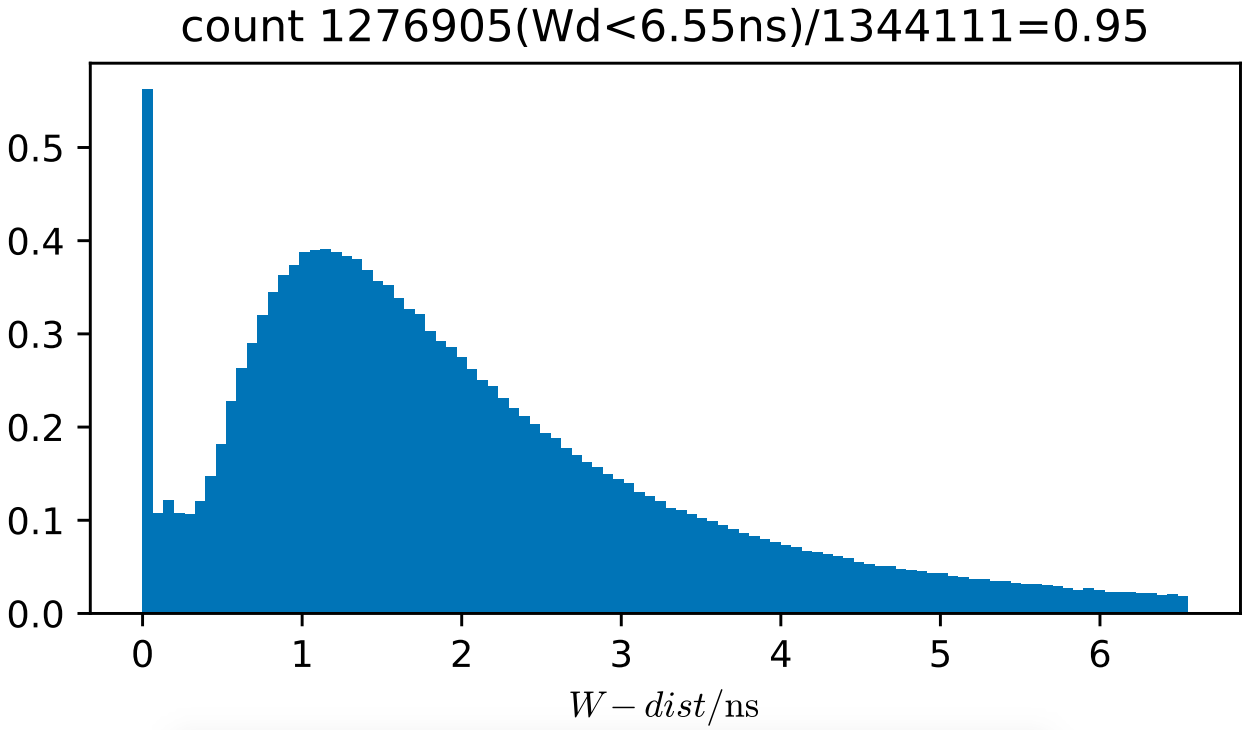
\includegraphics[width=1.0\textwidth]{figures/xiaopeippenumhist.png}
    \caption{$W_{d}$ Histogram when fitting $n_{r}$}
\end{figure}
\end{minipage}
\begin{minipage}{.5\textwidth}
\begin{figure}[H]
    \centering
        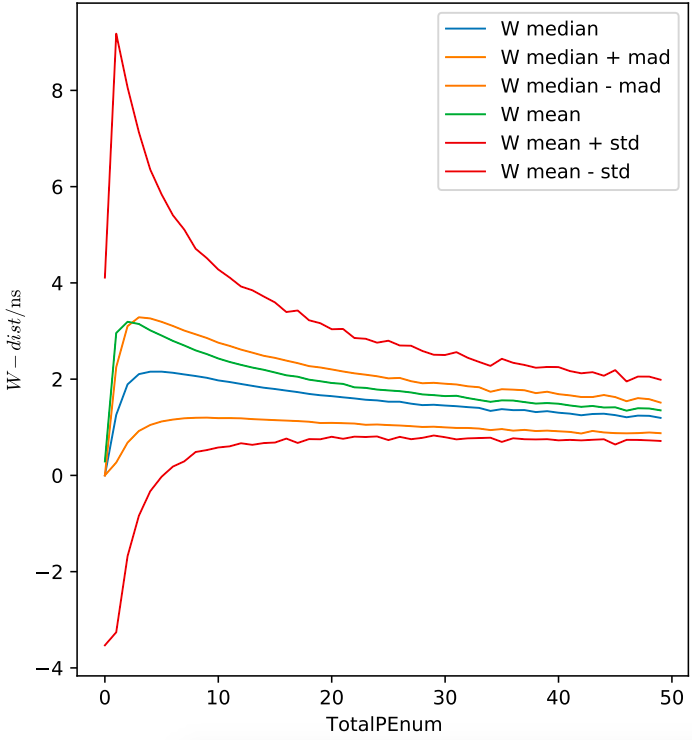
\includegraphics[width=0.7\textwidth]{figures/xiaopeippenumstats.png}
    \caption{$W_{d}$ vs $N_{pe}$ when fitting $n_{r}$}
\end{figure}
\end{minipage}
\end{figure}
\begin{figure}[H]
\begin{minipage}{.5\textwidth}
\begin{figure}[H]
    \centering
        \includegraphics[width=1.0\textwidth]{figures/xiaopeipchargehist.png}
    \caption{$W_{d}$ Histogram when fitting $q_{r}$}
\end{figure}
\end{minipage}
\begin{minipage}{.5\textwidth}
\begin{figure}[H]
    \centering
        \includegraphics[width=0.7\textwidth]{figures/xiaopeipchargestats.png}
    \caption{$W_{d}$ vs $N_{pos}$ when fitting $q_{r}$}
\end{figure}
\end{minipage}
\end{figure}

% \subsection{CNN}
\subsection{CNN}

\subsubsection{Network structure}
%\subsection{What is a good Network Structure?} 

Advances in neural networks have brought breakthroughs in various domains like Computer Vision and Natural Language Processing. As an efficient composition with weighted additions and pointwise nonlinearities, the method has prevailed against most of the traditional algorithms in pattern recognition tasks. In our experiment, we introduced a multi-layer convolutional neural network to process time-sensitive signals from detector outputs. Based on the Physics nature that a detector signal (PMT outputs) do only have a local correlation with recent incoming particles (photons incidents), we chose convolutional setups with a moderate total width coverage. From a view of information, a broader coverage by an output neuron's receptive field on its related area will contribute to higher accuracy, while redundant connections could only lead to excessive computation and lower processing speed. As a result, a wise setup should try to cover all relevant signal areas exclusively while cutting off every connection unnecessary, balancing the speed and accuracy from the two mentioned effects.

A similar trade-off also exists in the depth of the neural network. A deeper network could provide more complex combinations to all detected features, and the computation complexity of result calculation changes linearly with the depth. With the existence of advanced structure like residual connection and strategies like batch-norm, depth in training is never a problem. However, to cut the computation in massive experimental data, a network should be relatively shallow. Detector signals are relatively similar and peak-shaped. Such a simple pattern does not require many layers to recognize. A good design for the task is a network with 4 to 6 layers. Deeper structures may bring a slight improvement in precision but will introduce a considerable increase in processing cost.

A convolutional neural network is developed to analys the waveform. Here is the structure of CNN which has 5 convolutional layer (see figure~\ref{fig:struct}). The length of data remains the same. 

\subsubsection{Processing workflow}
%\subsection{What is a complete workflow of Data Processing?}
The complete workflow of data processing consists of two stages, data training and predicting. Data training is a task of supervised learning.  Based on paired data examples, the goal is to find an efficient mapping from detector waves to particle incidents with backpropagation methods. In the training process, a loss function judges the difference between training outputs and their referenced truth, and the training process is to minimize the loss. The product of network training is a function that creates desired outputs from inputs. By directly putting waveforms as inputs, one can get demanded outputs from a trained network in prediction.
%<Add a workflow description here>

\subsubsection{Loss function}
%\subsection{What is a good Loss Function?}
A critical issue matters the network training is the loss function. Particle incidence only happens in a small proportion of time channels within a recorded sequence, which means the outputs and related truth are always sparse. While operating with ineffective loss functions, training processes always ends up in local optimal of constant output due to the sparsity. Also, in practice, the form of loss function influence heavily on the final prediction performance. 

A well-designed loss function should meet two requirements as follows: it should handle the sparsity, and it should give a fair judgement to the output in training. A qualified loss function could work on either sequence values or normalized distributions. In pursuit of time precision, a good algorithm should encourage correct predictions in the close neighbourhoods of their corresponding truth, while punishing outputs that are incorrect or inaccurate in time. While working on the sequence outputs, such a mechanism is easy to implement but hard to arrange appropriately. It is hard to find a fair arrangement of punishment weight matching all circumstance. On the other hand, statistical distances and divergences could assess the difference in distribution but are hard to implement in a trainable form for backpropagation. 

To tackle the mentioned difficulties, efforts of our work have established feasible, robust solutions with guaranteed performance and convergence for each case of processing. We will describe the details of the method in the following section.

\emph{Value-based Reconstruction Loss}
% Introductory Photos should be added to this part.
To cope with sparsity in value-based processing, we have introduced a reconstruction procedure to build up a waveform based on its corresponding particle incidences. By introducing a reverse process after neural network computing, one could define the loss function on a denser wave domain instead of the original incidence domain. Expression of the reconstruction is arbitrary but should fit the paired relationship expressed by data samples. Typically, one should add a training process to fit the parameters in construction expressions before training the predicting neural networks.
%<Add an algorithm description here>

\emph{CDF Wasserstein Loss}
A direct implementation of judgement metrics into loss function is often difficult. To deal with sparsity and encourage time accuracy, we established the loss function on the cumulative distribution functions (CDF) of normalized outputs. The form of cumulative sums could build a connection between sequence prediction and its previous values, making optimization through history possible. Moreover, the first Wasserstein distance between two 1D distributions is equivalent to the norm-1 difference of two corresponding CDFs. The optimal transport amount described by this metric is a reliable measurement standard to all distribution differences, including cases in our application.

\begin{figure}[H]
\begin{minipage}{.3\textwidth}
\begin{figure}[H]
    \centering
    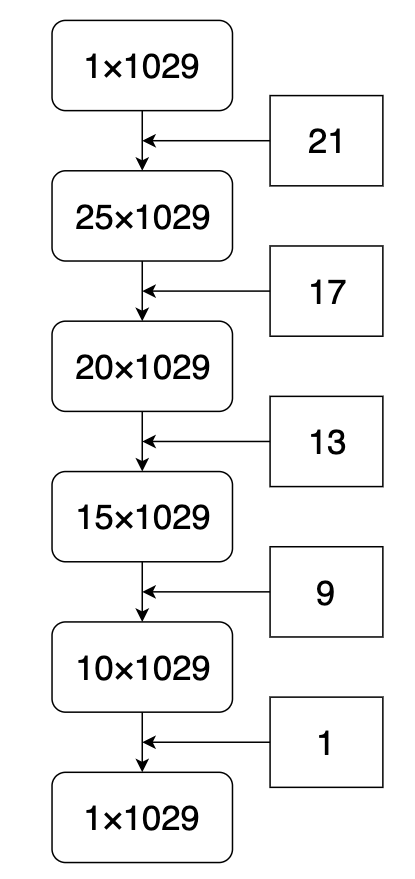
\includegraphics[width=0.8\textwidth]{figures/model.png}
    \caption{\label{fig:struct} CNN Structure}
\end{figure}
\end{minipage}
\hspace{4mm}
\begin{minipage}{.7\textwidth}
\lstinputlisting[language=Python, basicstyle=\small]{figures/CNN}
\end{minipage}
\end{figure}

\subsubsection{Result}
In the training process, we trained CNN for each PMT channel. The loss which is Wasserstein distance during training show in figure \ref{fig:loss}. 

\begin{figure}[H]
    \centering
    \scalebox{0.4}{version https://git-lfs.github.com/spec/v1
oid sha256:73951bc6ffdd6eeb65da3a90d8fe1d632cd9229743e7cf4c70a83604012baa97
size 35431
}
    \caption{\label{fig:loss} Loss variation during training}
\end{figure}

The result shows that CNN is the best for reconstruction of $q_{r}(t_{H})$ and $n_{r}(t_{H})$. 

\begin{figure}[H]
\begin{minipage}{.5\textwidth}
\begin{figure}[H]
    \centering
        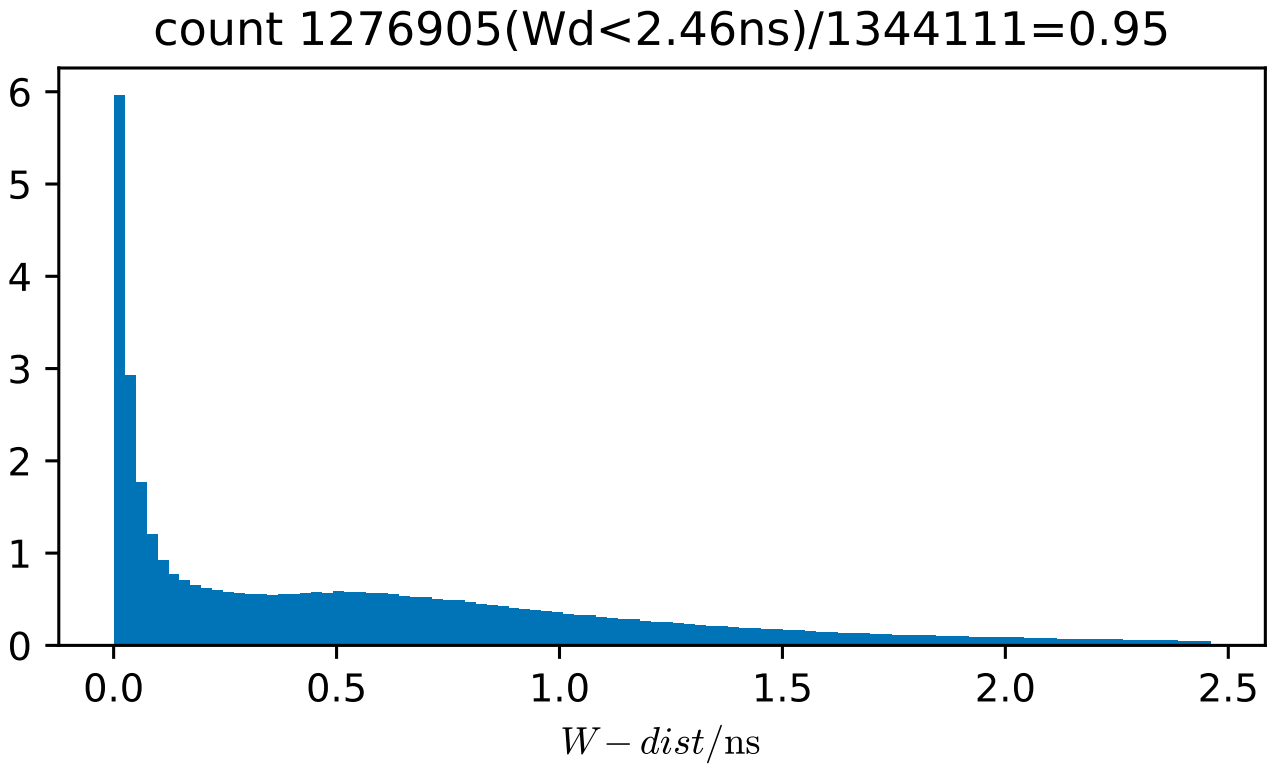
\includegraphics[width=1.0\textwidth]{figures/takarapenumhist.png}
    \caption{$W_{d}$ Histogram when CNN $n_{r}$}
\end{figure}
\end{minipage}
\begin{minipage}{.5\textwidth}
\begin{figure}[H]
    \centering
        \includegraphics[width=0.7\textwidth]{figures/takarapenumstats.png}
    \caption{$W_{d}$ vs $N_{pe}$ when CNN $n_{r}$}
\end{figure}
\end{minipage}
\end{figure}
\begin{figure}[H]
\begin{minipage}{.5\textwidth}
\begin{figure}[H]
    \centering
        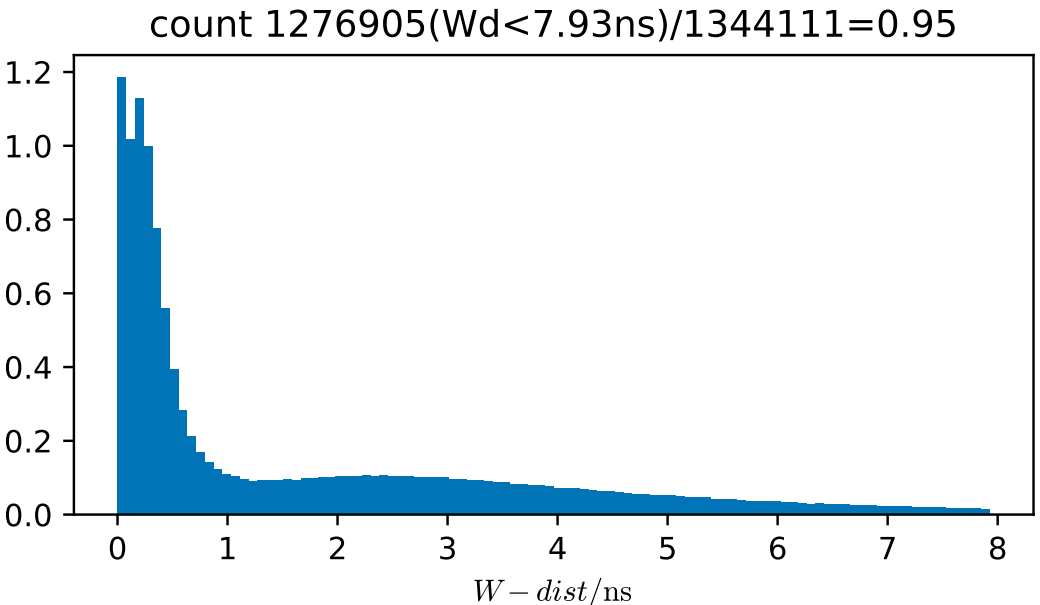
\includegraphics[width=1.0\textwidth]{figures/takarachargehist.png}
    \caption{$W_{d}$ Histogram when CNN $q_{r}$}
\end{figure}
\end{minipage}
\begin{minipage}{.5\textwidth}
\begin{figure}[H]
    \centering
        \includegraphics[width=0.7\textwidth]{figures/takarachargestats.png}
    \caption{$W_{d}$ vs $N_{pos}$ when CNN $q_{r}$}
\end{figure}
\end{minipage}
\end{figure}

% section Algorithm (end)